% !TEX program = xelatex
%=============================================================================
% MÉMOIRE DE MASTER — GÉNIE LOGICIEL
% RohWinBghit — Plateforme de covoiturage inter-wilayas en Algérie
% Université Abou Bakr Belkaid – Tlemcen · 2025/2026
% Auteurs : AHMED BACHA Djamel Eddine · BELHORMA Sidi Mohammed Reduane
% Encadrante : Mme BENLEDGHEM Rafika
% Compilation : xelatex memoire_rohwinbghit.tex (2 passes)
%=============================================================================

\documentclass[12pt, a4paper, oneside]{report}

% ---------- Hyperliens ----------
\usepackage{hyperref}
\hypersetup{
  colorlinks=true,
  linkcolor=rohblue,
  citecolor=rohblue,
  urlcolor=rohblue,
  pdftitle={RohWinBghit - Memoire Master Genie Logiciel},
  pdfauthor={AHMED BACHA Djamel Eddine, BELHORMA Sidi Mohammed Reduane}
}

% ---------- Acronymes ----------
\usepackage[acronym,nonumberlist]{glossaries}
\makeglossaries
% Liste des acronymes et abréviations
\newacronym{aes}{AES}{Advanced Encryption Standard (chiffrement symétrique 256 bits)}
\newacronym{aiia}{AI / IA}{Artificial Intelligence / Intelligence Artificielle}
\newacronym{api}{API}{Application Programming Interface}
\newacronym{apns}{APNs}{Apple Push Notification service}
\newacronym{asgi}{ASGI}{Asynchronous Server Gateway Interface (FastAPI)}
\newacronym{bdd}{BDD}{Base De Données}
\newacronym{bcrypt}{BCrypt}{Blowfish Cryptographic Hash Function (hachage mots de passe)}
\newacronym{cib}{CIB}{Carte Interbancaire (carte bancaire nationale algérienne)}
\newacronym{crud}{CRUD}{Create, Read, Update, Delete}
\newacronym{css}{CSS}{Cascading Style Sheets}
\newacronym{cv2}{CV2}{OpenCV (bibliothèque vision par ordinateur Python)}
\newacronym{dz}{DZ}{Algérie (code pays ISO 3166-1 alpha-2)}
\newacronym{erd}{ERD}{Entity-Relationship Diagram}
\newacronym{fcm}{FCM}{Firebase Cloud Messaging (notifications push Android)}
\newacronym{gps}{GPS}{Global Positioning System}
\newacronym{hog}{HOG}{Histogram of Oriented Gradients (descripteur visuel)}
\newacronym{html}{HTML}{HyperText Markup Language}
\newacronym{http}{HTTP}{HyperText Transfer Protocol}
\newacronym{httphttps}{HTTP/HTTPS}{HyperText Transfer Protocol / Secure}
\newacronym{ide}{IDE}{Integrated Development Environment}
\newacronym{ios}{iOS}{iPhone Operating System}
\newacronym{json}{JSON}{JavaScript Object Notation}
\newacronym{jwt}{JWT}{JSON Web Token (authentification sans état)}
\newacronym{kyc}{KYC}{Know Your Customer (vérification réglementaire d'identité)}
\newacronym{mcd}{MCD}{Modèle Conceptuel de Données}
\newacronym{mld}{MLD}{Modèle Logique de Données}
\newacronym{mvc}{MVC}{Model-View-Controller}
\newacronym{mvp}{MVP}{Minimum Viable Product}
\newacronym{orm}{ORM}{Object-Relational Mapping}
\newacronym{otp}{OTP}{One-Time Password}
\newacronym{pkfk}{PK / FK}{Primary Key / Foreign Key (clé primaire / étrangère)}
\newacronym{rbac}{RBAC}{Role-Based Access Control}
\newacronym{redis}{Redis}{Remote Dictionary Server (base de données clé-valeur en mémoire)}
\newacronym{rest}{REST}{Representational State Transfer}
\newacronym{sdk}{SDK}{Software Development Kit}
\newacronym{spa}{SPA}{Single Page Application}
\newacronym{sql}{SQL}{Structured Query Language}
\newacronym{swr}{SWR}{Stale-While-Revalidate (stratégie de cache)}
\newacronym{sgbd}{SGBD}{Système de Gestion de Base de Données}
\newacronym{tls}{TLS}{Transport Layer Security}
\newacronym{sms}{SMS}{Short Message Service}
\newacronym{ui}{UI}{User Interface}
\newacronym{uml}{UML}{Unified Modeling Language}
\newacronym{url}{URL}{Uniform Resource Locator}
\newacronym{uuid}{UUID}{Universally Unique Identifier}
\newacronym{ux}{UX}{User eXperience}
\newacronym{vtc}{VTC}{Véhicule de Tourisme avec Chauffeur}
\newacronym{wsgi}{WSGI}{Web Server Gateway Interface (Python sync)}
\newacronym{2fa}{2FA}{Two-Factor Authentication}
\newacronym{bmc}{BMC}{Business Model Canvas}
\newacronym{swot}{SWOT}{Strengths, Weaknesses, Opportunities, Threats}
\newacronym{sus}{SUS}{System Usability Scale}
\newacronym{sarl}{SARL}{Société à Responsabilité Limitée}
\newacronym{cnl}{CNL}{Comité National Label}
\newacronym{etp}{ETP}{Équivalent Temps Plein}
\newacronym{anpdp}{ANPDP}{Autorité Nationale de Protection des Données à Caractère Personnel}
\newacronym{vps}{VPS}{Virtual Private Server}
\newacronym{cac}{CAC}{Coût d'Acquisition Client}
\newacronym{arpu}{ARPU}{Average Revenue Per User}
\newacronym{kpi}{KPI}{Key Performance Indicator}
\newacronym{cin}{CIN}{Carte d'Identité Nationale}
\newacronym{idor}{IDOR}{Insecure Direct Object Reference}
\newacronym{og}{OG}{Objectif Général}
\newacronym{os}{OS}{Objectif Spécifique}


% ---------- Encodage et langues ----------
\usepackage{fontspec}
\usepackage{polyglossia}
\setmainlanguage{french}
\setotherlanguage{arabic}

\TeXXeTstate=1
\newfontfamily\arabicfont[Script=Arabic,Scale=1.1,Extension=.ttf,UprightFont=Amiri-Regular,BoldFont=Amiri-Bold,ItalicFont=Amiri-Italic,BoldItalicFont=Amiri-BoldItalic]{Amiri-Regular}

% ---------- Mise en page ----------
\usepackage[top=2.5cm,bottom=2.5cm,left=3cm,right=2cm]{geometry}
\setlength{\headheight}{15.21004pt}
\addtolength{\topmargin}{-3.21004pt}
\usepackage{setspace}
\onehalfspacing
\setlength{\parindent}{1.25em}
\usepackage{microtype}

% ---------- Graphisme et couleurs ----------
\usepackage{graphicx}
\graphicspath{{figures/}{./}}
\usepackage[table]{xcolor}
\definecolor{rohblue}{RGB}{30,80,150}
\definecolor{rohlight}{RGB}{235,242,250}
\definecolor{rohaccent}{RGB}{200,60,60}

% Anciennes couleurs pour compatibilité
\definecolor{bmcblue}{RGB}{52,103,158}
\definecolor{bmclight}{RGB}{235,242,250}

% ---------- Tableaux ----------
\usepackage{array}
\usepackage{tabularx}
\usepackage{longtable}
\usepackage{booktabs}
\usepackage{multirow}
\usepackage{colortbl}

% ---------- Listes et divers ----------
\usepackage{enumitem}
\usepackage{float}
\usepackage{caption}
\usepackage{subcaption}
\captionsetup[figure]{labelfont={it,bf},textfont=it,labelsep=endash,font=small}
\captionsetup[table]{labelfont={it,bf},textfont=it,labelsep=endash,font=small}

\usepackage{amsmath}
\usepackage{amssymb}
\usepackage{pifont}
\newcommand{\cmark}{\ding{51}}
\newcommand{\xmark}{\ding{55}}
\usepackage{soul}
\usepackage{ulem}
\normalem

% ---------- Titres de chapitres ----------
\usepackage[explicit]{titlesec}
\titleformat{\chapter}[display]
  {\normalfont\huge\bfseries\color{rohblue}}
  {\filleft\Large\scshape Chapitre \thechapter}
  {0pt}
  {\vspace{0.4em}\filleft\Huge #1\vspace{-0.3em}\color{rohblue}\titlerule[1pt]}
\titlespacing*{\chapter}{0pt}{10pt}{40pt}

\titleformat{\section}
  {\color{rohblue}\Large\bfseries}{\thesection}{0.6em}{#1}
\titleformat{\subsection}
  {\color{rohblue!85}\large\bfseries}{\thesubsection}{0.6em}{#1}
\titleformat{\subsubsection}
  {\color{rohblue!70}\normalsize\bfseries}{\thesubsubsection}{0.6em}{#1}

% ---------- En-têtes / pieds de page ----------
\usepackage{fancyhdr}
\pagestyle{fancy}
\fancyhf{}
\fancyhead[L]{\nouppercase{\leftmark}}
\fancyhead[R]{\thepage}
\renewcommand{\headrulewidth}{0.4pt}
\fancypagestyle{plain}{\fancyhf{}\fancyfoot[C]{\thepage}\renewcommand{\headrulewidth}{0pt}}

% ---------- Code source ----------
\usepackage{listings}
\definecolor{codegray}{rgb}{0.5,0.5,0.5}
\definecolor{codepurple}{rgb}{0.58,0,0.82}
\definecolor{codeblue}{rgb}{0.13,0.29,0.53}
\definecolor{backcolour}{rgb}{0.97,0.97,0.97}
\lstset{
  basicstyle=\ttfamily\small,
  keywordstyle=\color{rohblue}\bfseries,
  commentstyle=\color{gray}\itshape,
  stringstyle=\color{rohaccent},
  numbers=left, numberstyle=\tiny\color{gray},
  frame=single, rulecolor=\color{rohblue!30},
  breaklines=true, showstringspaces=false,
  tabsize=2
}
\lstdefinestyle{jsstyle}{
    backgroundcolor=\color{backcolour},
    commentstyle=\color{codegray}\itshape,
    keywordstyle=\color{codeblue}\bfseries,
    stringstyle=\color{codepurple},
    basicstyle=\ttfamily\small,
    breaklines=true, numbers=left,
    numberstyle=\tiny\color{codegray},
    frame=single, tabsize=2
}

% ---------- Encadrés ----------
\usepackage{tcolorbox}
\tcbuselibrary{skins,breakable}
\newtcolorbox{highlight}[1][]{
  enhanced, breakable,
  colback=rohlight, colframe=rohblue,
  boxrule=0.5pt, arc=2pt,
  left=8pt,right=8pt,top=5pt,bottom=5pt,
  #1
}
\definecolor{funcgreen}{RGB}{200,230,201}
\definecolor{funcgreendark}{RGB}{46,125,50}
\newtcolorbox{funcreq}[1][]{
  enhanced, breakable,
  colback=funcgreen!40, colframe=funcgreendark,
  boxrule=0.6pt, arc=2pt,
  left=8pt,right=8pt,top=5pt,bottom=5pt,
  title={\textbf{Exigence fonctionnelle}},
  fonttitle=\bfseries\color{white},
  colbacktitle=funcgreendark,
  #1
}
\definecolor{nonfuncorange}{RGB}{255,224,178}
\definecolor{nonfuncorangedark}{RGB}{230,81,0}
\newtcolorbox{nonfuncreq}[1][]{
  enhanced, breakable,
  colback=nonfuncorange!40, colframe=nonfuncorangedark,
  boxrule=0.6pt, arc=2pt,
  left=8pt,right=8pt,top=5pt,bottom=5pt,
  title={\textbf{Exigence non fonctionnelle}},
  fonttitle=\bfseries\color{white},
  colbacktitle=nonfuncorangedark,
  #1
}

%=============================================================================
\usepackage[backend=biber,style=ieee,sorting=none]{biblatex}
\addbibresource{biblio.bib}
\begin{document}
%=============================================================================

%─── Page de garde ────────────────────────────────────────────────────────────
\begin{titlepage}
\centering
{\large \textbf{REPUBLIQUE ALGERIENNE DEMOCRATIQUE ET POPULAIRE}}\\[3pt]
{\small Ministere de l'Enseignement Superieur et de la Recherche Scientifique}\\[6pt]
{\large \textbf{Universite Abou Bakr Belkaid --- Tlemcen}}\\
{\normalsize Faculte des Sciences --- Departement d'Informatique}\\[1.5em]
\rule{\textwidth}{1.5pt}\\[0.8em]
{\LARGE \textbf{Memoire de Fin d'Etudes}}\\[4pt]
{\large \emph{Pour l'obtention du diplome de \textbf{Master}}}\\
{\large Option : \textbf{Genie Logiciel (G.L)}}\\[0.8em]
\rule{\textwidth}{1.5pt}\\[1.8em]
{\huge \textbf{Ingenierie et mise en oeuvre d'une plateforme}}\\[4pt]
{\huge \textbf{multi-plateforme de covoiturage inter-wilayas}}\\[8pt]
{\LARGE \textit{\textbf{(RohWinBghit)}}}\\[2.5em]
\begin{minipage}{0.48\textwidth}
\raggedright
\textbf{Realisee par :}\\[2pt]
\quad --- AHMED BACHA Djamel Eddine\\
\quad --- BELHORMA Sidi Mohammed Reduane\\[1.5em]
\textcolor{blue!70!black}{\textbf{Projet labellisé Startup par le Ministère}}\\
\textcolor{blue!70!black}{\textbf{de l'Économie du Savoir, Startups et Micro-Entreprises}}
\end{minipage}
\hfill
\begin{minipage}{0.48\textwidth}
\raggedleft
\textbf{Encadrante :}\\[2pt]
Mme BENLEDGHEM Rafika
\end{minipage}\\[3em]
\begin{tabular}{ll}
Mr. \underline{\hspace{7cm}} & President \\[4pt]
Mr. \underline{\hspace{7cm}} & Examinateur \\[4pt]
Mme BENLEDGHEM Rafika & Encadrante \\[4pt]
Mr. \underline{\hspace{7cm}} & Expert \\
\end{tabular}\\[2.5em]
{\large \textbf{Annee universitaire 2025/2026}}
\end{titlepage}

%─── Tables ───────────────────────────────────────────────────────────────────
\tableofcontents
\newpage
\listoffigures
\newpage
\listoftables
\newpage


\chapter*{Dédicace}
\addcontentsline{toc}{chapter}{Dédicaces}

Je dédie ce travail à mes chers parents, pour leur amour inconditionnel, leur soutien sans faille et les sacrifices consentis tout au long de mon parcours universitaire. Chaque ligne de ce mémoire porte l'empreinte de leurs encouragements constants.

À mes frères et sœurs, pour leur présence réconfortante et leur foi inébranlable en mes capacités. À mes amis et collègues de promotion, pour les moments de solidarité et de partage qui ont rendu ces années d'étude plus riches et plus mémorables.

À mon binôme Reduane, dont la rigueur, la passion pour le code et l'esprit d'initiative ont été des sources d'inspiration permanentes tout au long de ce projet. Ce mémoire est aussi le fruit de notre collaboration technique et humaine.

\emph{Djamel Eddine}

\chapter*{Dédicace}
\addcontentsline{toc}{chapter}{Dédicaces}

Je dédie ce mémoire à mes chers parents, à ma mère pour son amour infini, sa patience et ses prières qui m'ont accompagné à chaque étape, et à mon père pour sa sagesse et sa confiance constante. Vous êtes et resterez ma plus grande source de motivation.

À mon frère et ma sœur, pour leur soutien moral et leur présence bienveillante dans les moments difficiles. À tous mes amis de promotion pour les souvenirs inoubliables et la solidarité qui ont marqué ces années universitaires.

À mon binôme Djamel Eddine, pour son engagement technique exemplaire, sa créativité dans la résolution de problèmes complexes et sa volonté constante de repousser les limites de ce que nous pouvions réaliser ensemble.

\emph{Sidi Mohammed Reduane}

\chapter*{Remerciements}
\addcontentsline{toc}{chapter}{Remerciements}

Au terme de ce travail, nous souhaitons exprimer notre profonde gratitude envers toutes les personnes qui ont contribué, directement ou indirectement, à l'aboutissement de ce projet ambitieux.

Nous remercions en premier lieu Dieu le Tout-Puissant de nous avoir accordé la santé, la volonté et la persévérance nécessaires pour mener à bien ce projet technique de grande envergure.

Nous exprimons notre gratitude la plus sincère à notre encadrante Mme BENLEDGHEM Rafika, Maître de Conférences au Département d'Informatique de l'Université Abou Bakr Belkaid -- Tlemcen, pour son suivi rigoureux, ses orientations techniques précieuses et son soutien constant tout au long du développement de cette plateforme.

Nous remercions les membres du jury pour l'honneur qu'ils nous font en évaluant ce travail, ainsi que l'ensemble des enseignants du Département d'Informatique pour la qualité de la formation dispensée.

Enfin, nos remerciements les plus chaleureux vont à nos familles respectives pour leur patience, leur compréhension et leur soutien moral indéfectible durant toutes ces années d'études.

\chapter*{\textarabic{ملخص}}
\addcontentsline{toc}{chapter}{\texorpdfstring{\textarabic{ملخص}}{Résumé (Arabe)}}

\begin{Arabic}
يهدف هذا المشروع إلى تصميم وتطوير منصة رقمية متعددة المنصات للنقل المشترك بين الولايات تحت اسم RohWinBghit. يتكون النظام من أربعة مشاريع فرعية: واجهة برمجية مبنية على Node.js وExpress وKnex، تطبيق جوال بـReact Native وExpo، واجهة ويب بـReact وVite، وخدمة ذكاء اصطناعي بـFastAPI لإجراء التحقق البيومتري.

تتميز المنصة بتكامل خمس طرق للدفع الإلكتروني (CIB، Edahabia، Stripe، PayPal، نقدي)، خوارزميات التسعير الديناميكي، اكتشاف الاحتيال، ونظام التحقق من الهوية بالذكاء الاصطناعي. أظهرت نتائج الاختبار أن الحل المقترح فعال وآمن وقابل للتوسع.

\textbf{الكلمات المفتاحية: النقل المشترك، Express.js، React Native، Zustand، PostgreSQL، FastAPI، التحقق البيومتري، التسعير الديناميكي.}
\end{Arabic}

\chapter*{Résumé}
\addcontentsline{toc}{chapter}{Résumé}

Le présent mémoire porte sur la conception et la réalisation de RohWinBghit, un écosystème multi-plateforme de covoiturage inter-wilayas composé de quatre sous-projets complémentaires : un backend Node.js/Express/Knex/PostgreSQL, une application mobile React Native/Expo, un frontend web React/Vite/TypeScript et un service d'intelligence artificielle FastAPI dédié à la vérification biométrique.

La plateforme intègre des fonctionnalités avancées dépassant largement les standards du secteur : trois méthodes de paiement opérationnelles (CIB, Edahabia en sandbox, espèces) extensibles via un pattern Factory (Stripe et PayPal prévus), un moteur de tarification dynamique (surge pricing), un système de détection de fraude en temps réel, un algorithme de scoring conducteur, et un service IA de vérification d'identité (reconnaissance faciale, détection de vivacité, anti-spoofing).

La base de données PostgreSQL est structurée autour de 35+ migrations documentant l'évolution complète du schéma. La sécurité est assurée par AES-256-GCM, bcrypt, JWT, rate limiting et monitoring Sentry. Les résultats des tests de validation confirment la robustesse et la scalabilité de la solution.

\textbf{Mots-clés :} covoiturage, Node.js, Express.js, Knex, PostgreSQL, React Native, Zustand, FastAPI, vérification biométrique, surge pricing, détection de fraude, RohWinBghit.

\chapter*{Abstract}
\addcontentsline{toc}{chapter}{Abstract}

This thesis presents the design and implementation of RohWinBghit, a multi-platform carpooling ecosystem for inter-wilaya travel in Algeria, composed of four complementary sub-projects: a Node.js/Express/Knex/PostgreSQL backend, a React Native/Expo mobile application, a React/Vite/TypeScript web frontend, and a FastAPI-based AI service dedicated to biometric identity verification.

The platform integrates advanced features well beyond sector standards: five electronic payment methods (CIB, Edahabia, Stripe, PayPal, cash) via a Factory design pattern, a dynamic pricing engine (surge pricing), a real-time fraud detection system, a driver scoring algorithm, and an AI identity verification service (facial recognition, liveness detection, anti-spoofing). The PostgreSQL database comprises 35+ migrations documenting the complete schema evolution.

\textbf{Keywords:} carpooling, Node.js, Express.js, Knex, PostgreSQL, React Native, Zustand, FastAPI, biometric verification, surge pricing, fraud detection, RohWinBghit.



\chapter*{Liste des abréviations}
\addcontentsline{toc}{chapter}{Liste des abréviations}

\textbf{AES} : Advanced Encryption Standard (chiffrement symétrique 256 bits)

\textbf{AI / IA} : Artificial Intelligence / Intelligence Artificielle

\textbf{API} : Application Programming Interface

\textbf{APNs} : Apple Push Notification service

\textbf{ASGI} : Asynchronous Server Gateway Interface (FastAPI)

\textbf{BCrypt} : Blowfish Cryptographic Hash Function (hachage mots de passe)

\textbf{CIB} : Carte Interbancaire (carte bancaire nationale algérienne)

\textbf{CRUD} : Create, Read, Update, Delete

\textbf{CV2} : OpenCV (bibliothèque vision par ordinateur Python)

\textbf{DZ} : Algérie (code pays ISO 3166-1 alpha-2)

\textbf{FCM} : Firebase Cloud Messaging (notifications push Android)

\textbf{GPS} : Global Positioning System

\textbf{HOG} : Histogram of Oriented Gradients (descripteur visuel)

\textbf{HTTP/HTTPS} : HyperText Transfer Protocol / Secure

\textbf{JWT} : JSON Web Token (authentification sans état)

\textbf{KYC} : Know Your Customer (vérification réglementaire d'identité)

\textbf{MCD} : Modèle Conceptuel de Données

\textbf{MLD} : Modèle Logique de Données

\textbf{ORM} : Object-Relational Mapping

\textbf{PK / FK} : Primary Key / Foreign Key (clé primaire / étrangère)

\textbf{RBAC} : Role-Based Access Control

\textbf{Redis} : Remote Dictionary Server (base de données clé-valeur en mémoire)

\textbf{REST} : Representational State Transfer

\textbf{SDK} : Software Development Kit

\textbf{SPA} : Single Page Application

\textbf{SQL} : Structured Query Language

\textbf{SWR} : Stale-While-Revalidate (stratégie de cache)

\textbf{TLS} : Transport Layer Security

\textbf{UML} : Unified Modeling Language

\textbf{UUID} : Universally Unique Identifier

\textbf{VTC} : Véhicule de Tourisme avec Chauffeur

\textbf{WSGI} : Web Server Gateway Interface (Python sync)


% --- Fused: introduction_generale.tex ---
\chapter*{Introduction générale}
\addcontentsline{toc}{chapter}{Introduction générale}
\markboth{Introduction générale}{}

\section*{Contexte et motivation}

La mobilité intercité constitue l'un des défis structurels majeurs de l'Algérie contemporaine. Avec une superficie de 2~381~741~km² répartie en 69 wilayas et une population dépassant 45~millions d'habitants, le pays présente un besoin constant de déplacements entre villes universitaires, pôles économiques et zones résidentielles. Les solutions traditionnelles --- taxis intercités, lignes de bus privées, véhicules personnels --- demeurent fragmentées, onéreuses et peu transparentes. Les étudiants, les travailleurs navetteurs et les familles sont les premiers pénalisés par cette offre inadéquate.

Parallèlement, la révolution numérique mondiale a vu émerger, depuis le milieu des années 2000, des plateformes de \textit{covoiturage} --- \textit{BlaBlaCar} en Europe, \textit{Via} aux États-Unis, \textit{Careem} et \textit{Yassir} au Moyen-Orient et en Afrique du Nord --- qui transforment les déplacements en services à la demande, plus économiques et plus sociaux. Pourtant, aucune solution adaptée au contexte algérien n'a atteint une couverture véritablement nationale~: les offres existantes sont soit centrées sur le transport urbain (\textit{Yassir}, \textit{Heetch}), soit absentes du trafic inter-wilayas.

Cette réalité a motivé la conception du projet \textbf{RohWinBghit} (\textarabic{روح وين بغيت}, littéralement \textit{«~va où tu veux~»}). Il s'agit d'une plateforme mobile distribuée offrant aux conducteurs algériens la possibilité de partager leurs trajets longue distance avec des passagers vérifiés, à travers une expérience sécurisée par une vérification biométrique d'identité, une géolocalisation temps réel et un moteur de paiement compatible avec les moyens locaux (CIB, Edahabia, espèces).

\section*{Problématique}

Comment concevoir et réaliser une plateforme mobile de covoiturage inter-wilayas spécifiquement adaptée au contexte algérien, capable simultanément~: (i)~d'instaurer un climat de confiance entre des utilisateurs qui ne se connaissent pas par le biais d'une vérification d'identité biométrique rigoureuse, (ii)~de garantir la disponibilité temps réel de l'offre et la fiabilité des trajets, (iii)~de supporter les moyens de paiement électroniques et informels propres au marché algérien, tout en s'appuyant sur une architecture logicielle moderne, extensible et conforme aux bonnes pratiques du génie logiciel~?

\section*{Objectifs du travail}

Le présent mémoire poursuit les objectifs suivants~:
\begin{enumerate}[leftmargin=1.8em]
  \item Analyser l'état de l'art du covoiturage numérique, les tendances technologiques associées, et positionner précisément la solution proposée par rapport aux acteurs existants.
  \item Identifier et formaliser les besoins fonctionnels et non fonctionnels d'une plateforme de covoiturage inter-wilayas adaptée à l'Algérie.
  \item Concevoir une architecture logicielle distribuée, extensible et maintenable, appuyée sur une modélisation UML rigoureuse (cas d'utilisation, séquences, classes, déploiement).
  \item Développer une application mobile multiplateforme (iOS / Android) accompagnée d'un \textit{back-end} performant et d'un service d'intelligence artificielle dédié à la vérification biométrique.
  \item Intégrer les moyens de paiement locaux (CIB, Edahabia) via un patron de conception \textit{Factory} garantissant l'extensibilité.
  \item Valider la solution par un plan de tests couvrant les fonctionnalités critiques et mesurer le taux de réussite.
  \item Élaborer un plan d'affaires (\textit{Business Model Canvas}, analyse SWOT, plan financier) démontrant la viabilité économique du projet.
\end{enumerate}

\section*{Cadre institutionnel --- Mécanisme «~Un diplôme, une Startup~» (Arrêté 1275)}

Ce mémoire s'inscrit dans le cadre du mécanisme national «~Un diplôme, une Startup~», institué par l'\textbf{Arrêté interministériel n\textsuperscript{o}~1275} du Ministère de l'Enseignement Supérieur et de la Recherche Scientifique (MESRS) en collaboration avec le Ministère délégué chargé des Startups et de l'Économie de la Connaissance. Ce dispositif permet à un étudiant inscrit en Master ou en Doctorat de valoriser son projet de fin d'études comme projet de création d'entreprise innovante, avec un accompagnement institutionnel allant de l'incubation jusqu'à l'obtention d'un label \textit{Startup} délivré par le MESRS.

Concrètement, \textit{RohWinBghit} répond aux trois critères d'éligibilité de l'Arrêté~1275~:\\
\begin{itemize}[leftmargin=2em]
  \item \textbf{Innovation technologique~:} la plateforme intègre un pipeline de vérification biométrique à base d'IA (détection de vivacité, anti-\textit{spoofing}) et une tarification dynamique fondée sur des données de marché en temps réel, deux éléments absents des solutions algériennes existantes.
  \item \textbf{Marché et viabilité économique~:} le Chapitre~4 démontre la viabilité du projet avec un \textit{business plan} complet (BMC, analyse SWOT, projections financières sur 36 mois, seuil de rentabilité au 10\textsuperscript{ème} mois).
  \item \textbf{Ancrage national~:} la solution est développée entièrement en Algérie, intègre les moyens de paiement locaux (CIB, Edahabia) et vise en priorité le marché algérien des 69~wilayas.
\end{itemize}

La démarche de dépôt auprès du Comité National Label (CNL) a été initiée, incluant l'enregistrement du nom commercial et de la marque auprès de l'\textbf{INAPI} (Institut National Algérien de la Propriété Industrielle) et la protection du code source auprès de l'\textbf{ONDA} (Office National des Droits d'Auteur). Les détails de la stratégie de propriété intellectuelle et du cadre juridique de la startup sont développés au Chapitre~4, Section~4.5.

\section*{Organisation du mémoire}

Ce mémoire est structuré en quatre chapitres, encadrés par une introduction générale et une conclusion générale~:

\begin{itemize}[leftmargin=1.8em]
  \item Le \textbf{Chapitre~1 --- Contexte général et étude de l'existant} dresse un panorama du covoiturage mondial et algérien, passe en revue les technologies clés (mobilité, intelligence artificielle, paiement électronique) et positionne \textit{RohWinBghit} à travers une étude comparative des solutions existantes. \textit{Méthodologiquement, ce chapitre s'appuie sur une recherche bibliographique et une analyse comparative fondée sur des critères fonctionnels et sécuritaires.}

  \item Le \textbf{Chapitre~2 --- Analyse et conception de la solution} présente la démarche méthodologique suivie, les acteurs du système, les besoins fonctionnels et non fonctionnels, et expose la modélisation UML complète. \textit{La démarche retenue s'appuie sur le processus unifié (UP), formalisée par des diagrammes de cas d'utilisation, de séquence, de classes, de déploiement, ainsi que par un dictionnaire de données détaillé.}

  \item Le \textbf{Chapitre~3 --- Réalisation, validation et sécurité du système} détaille l'environnement de développement, la pile technologique retenue, l'architecture des modules critiques (paiement, vérification biométrique), la stratégie de tests et les contre-mesures de sécurité. \textit{L'approche adoptée repose sur une implémentation itérative avec React Native et Node.js, validée par une suite de tests automatisés (Jest) et illustrée par une cartographie visuelle des parcours utilisateurs.}

  \item Le \textbf{Chapitre~4 --- Étude technico-économique et faisabilité du projet} propose une analyse stratégique, une étude de marché et un plan de production. \textit{Sur le plan méthodologique, ce chapitre mobilise la matrice SWOT pour l'analyse stratégique, des projections financières quantitatives pour l'étude de rentabilité, et le Business Model Canvas (BMC) pour synthétiser le modèle économique du projet.}
\end{itemize}

Enfin, la \textbf{conclusion générale} dresse le bilan des réalisations, discute les difficultés rencontrées et dessine les perspectives d'évolution du projet.


% --- Fused: chap1_etat_art.tex ---
\chapter{Contexte général et étude de l'existant}
\label{chap:etat-art}

\section*{Introduction}

Toute démarche d'ingénierie logicielle commence par une lecture attentive du terrain sur lequel la solution est appelée à s'inscrire. Le présent chapitre poursuit cette ambition à propos du projet \textit{RohWinBghit}, plateforme mobile de covoiturage inter-wilayas pensée pour l'Algérie. Nous y replaçons d'abord le projet dans la trajectoire plus large de la mobilité numérique mondiale, avant d'examiner les particularités du transport longue distance en Algérie et les opportunités offertes par un marché numérique en pleine expansion. Nous présentons ensuite les technologies clés mobilisées --- développement mobile multiplateforme, vérification d'identité par intelligence artificielle, paiement électronique local --- puis une étude comparative des solutions existantes, avant d'identifier les limites observables et de formuler le positionnement stratégique de notre proposition.

\section{Évolution de la mobilité numérique}
\label{sec:mobilite-numerique}

L'essor des réseaux mobiles a transformé en moins de deux décennies notre rapport au déplacement. Le passage du \textsc{gprs} (171~kbps) à la 4G \textsc{lte} (jusqu'à 150~Mbps), puis à la 5G, a rendu possibles des usages auparavant inenvisageables~: cartographie temps réel, paiement instantané, vérification biométrique en mobilité, messagerie multimédia~\cite{arpt_2024}. Cette évolution s'est accompagnée d'une démocratisation rapide du \textit{smartphone}~: aujourd'hui omniprésent, il intègre nativement les briques techniques --- \gls{gps}, accéléromètre, caméra de qualité, stockage sécurisé --- nécessaires aux applications de mobilité partagée modernes.

Cette convergence \textit{réseau + terminal} a redéfini l'architecture des services de transport. Les premières applications mobiles, simples vitrines de services existants, ont laissé place à des plateformes complètes coordonnant en temps réel l'offre et la demande, le paiement, la communication et la confiance entre utilisateurs. Le covoiturage, longtemps cantonné à des annonces statiques sur des sites \textit{web}, s'inscrit pleinement dans ce mouvement~: il est devenu, en quelques années, l'un des cas d'usage les plus représentatifs de cette mobilité numérique de nouvelle génération.

\section{Définition et intérêt du covoiturage}
\label{sec:definition-covoiturage}

\subsection{Concept et origine}

Le covoiturage (\textit{carpooling}, \textit{ridesharing}) désigne le partage d'un véhicule privé entre un conducteur et un ou plusieurs passagers réalisant un trajet similaire, moyennant un partage des frais. Apparu dès la Seconde Guerre mondiale aux États-Unis, sous l'effet du rationnement de carburant, il s'est structuré dans les années~1970 en réponse au choc pétrolier, avant de prendre sa forme contemporaine au cours des années~2000 avec l'émergence d'Internet, puis du \textit{smartphone}~\cite{chan_carpooling_2012}. L'arrivée de plateformes telles que \textit{BlaBlaCar} (France, 2006) a marqué l'industrialisation du modèle, en facilitant la mise en relation à grande échelle et en introduisant des mécanismes de confiance numérique.

\subsection{Bénéfices observés}

Lorsqu'il est correctement encadré par une plateforme numérique, le covoiturage produit une triple valeur~:
\begin{itemize}
  \item \textbf{Économique~:} mutualisation des frais (carburant, péages, amortissement). Les études européennes estiment à environ 40\,\% l'économie réalisée par passager sur un trajet longue distance~\cite{blablacar_report_2023}.
  \item \textbf{Sociale~:} accessibilité accrue aux zones mal desservies, lien intergénérationnel, démocratisation des déplacements pour les étudiants et les actifs à faibles revenus.
  \item \textbf{Environnementale~:} réduction du nombre de véhicules en circulation. L'\textsc{ademe} estime qu'un passager covoituré régulièrement évite en moyenne 110~kg de CO\textsubscript{2} par an~\cite{ademe_2022}.
\end{itemize}

\section{Situation du transport inter-wilayas en Algérie}
\label{sec:transport-algerie}

L'Algérie présente une géographie singulière~: un territoire de plus de 2,38~millions de km\textsuperscript{2}, structuré en 58~wilayas, et marqué par une concentration urbaine sur le littoral. Les déplacements inter-wilayas restent donc fortement dépendants de la voiture individuelle et de l'autocar, dans un contexte où le réseau ferroviaire ne dessert qu'une part limitée du territoire. Plusieurs constats récurrents émergent du terrain~:
\begin{itemize}
  \item Une forte demande étudiante hebdomadaire entre wilayas universitaires (Tlemcen, Oran, Constantine, Sétif, Alger) et wilayas d'origine.
  \item Une offre d'autocars saturée aux périodes de pointe, avec un confort et une ponctualité inégaux.
  \item Un coût du carburant relativement bas, mais un coût total de possession d'un véhicule en hausse, qui rend la mutualisation économiquement attractive.
  \item Une absence persistante de plateforme nationale offrant une expérience comparable aux standards internationaux pour les longues distances.
\end{itemize}

Le segment inter-wilayas constitue de ce fait un espace pertinent pour une plateforme numérique dédiée, complémentaire des solutions urbaines déjà installées (Yassir, Heetch).

\section{Opportunité du marché numérique algérien}
\label{sec:opportunite-marche}

Le marché algérien de la mobilité numérique est émergent mais dynamique. Les données publiées par l'Autorité de Régulation de la Poste et des Communications Électroniques (\textsc{arpt}) confirment cette tendance~\cite{arpt_2024}~: le taux de pénétration du \textit{smartphone} dépasse désormais 75\,\%, et le pays comptait plus de 48~millions d'abonnements Internet mobile actifs en 2024, soit environ 108~abonnements pour 100~habitants. Cette densité numérique élevée constitue un terrain favorable au déploiement d'applications mobiles de mobilité.

L'écosystème des paiements électroniques s'est lui aussi structuré ces dernières années. L'Algérie dispose désormais de deux cartes interbancaires majeures --- \textbf{CIB} (réseau bancaire commercial) et \textbf{Edahabia} (Algérie Poste) --- complétées par l'application de paiement mobile \textit{Baridi~Mob}. D'après les chiffres communiqués par l'Agence Presse Service, plus de \textbf{7~millions d'opérations} de paiement électronique ont été enregistrées sur les seuls premiers mois de 2025~\cite{aps_epaiement_2025}, témoignant d'une adoption en forte progression.

Le contexte démographique renforce cette opportunité~: le pays compte plus de 1,7~million d'étudiants inscrits dans l'enseignement supérieur, dont une part importante se déplace régulièrement entre leur wilaya d'origine et leur lieu d'études. Cette population, à la fois mobile et numériquement équipée, constitue une base initiale naturelle pour une plateforme inter-wilayas.

\section{Technologies clés mobilisées}
\label{sec:technologies}

\subsection{Développement mobile multiplateforme}

Le développement mobile s'organise aujourd'hui autour de deux grandes approches~: le \textit{natif} (Swift pour iOS, Kotlin pour Android) et le \textit{multiplateforme}. Dans cette seconde catégorie, les frameworks \textit{React Native} (Meta, 2015), \textit{Flutter} (Google, 2017) et \textit{Ionic} dominent l'écosystème. \textit{React Native} s'impose comme une solution de référence lorsque l'on recherche un compromis entre performance proche du natif, large écosystème JavaScript/TypeScript et délai réduit de mise sur le marché. Son modèle de \textit{pont} JavaScript-natif permet de mutualiser jusqu'à 95\,\% du code entre iOS et Android tout en exposant les capacités matérielles (GPS, caméra, notifications, stockage sécurisé) requises par une application de covoiturage.

\subsection{Vérification d'identité par intelligence artificielle (KYC)}

La vérification \gls{kyc} est devenue une étape incontournable pour toute plateforme manipulant des paiements ou organisant la rencontre physique entre inconnus. Elle repose sur trois briques techniques complémentaires~:
\begin{itemize}
  \item \textbf{Reconnaissance optique de caractères (OCR)} pour l'extraction structurée des données d'une pièce d'identité.
  \item \textbf{Reconnaissance faciale}, qui compare la photo du document à un \textit{selfie} fourni en temps réel.
  \item \textbf{Détection de vivacité} (\textit{liveness detection}), destinée à empêcher les attaques par présentation (photo imprimée, vidéo rejouée, masque). Les approches modernes reposent sur des réseaux de neurones convolutifs entraînés sur des bases de référence telles que \textit{CASIA-FASD} ou \textit{CelebA-Spoof}~\cite{boulkenafet_liveness_2017}.
\end{itemize}

\subsection{Paiement électronique local}

À l'échelle internationale, le paiement mobile s'est démocratisé via des solutions comme \textit{Apple~Pay}, \textit{Google~Pay}, \textit{Stripe} ou \textit{PayPal}. Pour le marché algérien, l'enjeu pratique réside dans l'intégration native des moyens de paiement locaux (CIB, Edahabia, Baridi~Mob), seule à même d'assurer une couverture financière suffisante pour les usagers réels.

\subsection{Géolocalisation et messagerie temps réel}

La précision GPS sub-métrique offerte par les \textit{smartphones} actuels, combinée à des services de cartographie tels que \textit{Mapbox} ou \textit{Google~Maps}, rend possible le suivi de trajet en temps réel et le calcul d'itinéraires optimisés. Côté communication, les protocoles \textit{WebSocket} (\textit{Socket.IO}) permettent une messagerie bidirectionnelle à faible latence, indispensable au chat conducteur--passager et aux notifications de statut.

\section{Étude comparative des solutions existantes}
\label{sec:comparatif}

Plusieurs plateformes de mobilité partagée opèrent aujourd'hui aux échelles internationale, régionale ou nationale. Pour positionner notre projet, nous avons retenu un échantillon représentatif et comparé ces plateformes selon huit critères jugés déterminants~: couverture géographique, présence sur le segment inter-wilayas, vérification d'identité, paiements locaux, messagerie temps réel, tarification dynamique, chiffrement des données et langues d'interface.

\subsection{Acteurs internationaux}

\textbf{BlaBlaCar} (France, 2006) reste la référence européenne du covoiturage longue distance, avec une présence dans 22~pays et plus de 100~millions d'utilisateurs cumulés. Son modèle, fondé sur le paiement en ligne et les notations croisées, n'est cependant pas adapté au contexte algérien (carte bancaire internationale requise, absence d'implantation locale). \textbf{IdVroom} (France), filiale de la \textsc{sncf}, s'est concentrée sur le covoiturage domicile--travail à l'échelle française. \textbf{Uber~Pool}, \textbf{Lyft~Shared} et \textbf{Via} (États-Unis) couvrent quant à eux le segment urbain partagé, sans offre inter-wilayas pertinente pour notre marché cible.

\subsection{Acteurs maghrébins et algériens}

Le marché algérien est aujourd'hui couvert par plusieurs acteurs urbains et, plus récemment, par deux acteurs sur le segment inter-wilayas.

\paragraph{Yassir.} Application algérienne fondée en 2017, \textit{Yassir} est devenue le leader local du \textsc{vtc} urbain. Une étude empirique récente conduite à Ali~Menjeli (Constantine) a montré que son adoption a réduit le temps d'attente moyen et transformé les pratiques de mobilité, y compris parmi les catégories les plus précaires~\cite{naim_yassir_2024}. Sa portée reste cependant urbaine.

\paragraph{Heetch.} Acteur français implanté en Algérie depuis 2020, également centré sur le segment urbain.

\paragraph{TemTem.} Plateforme algérienne de livraison et de \textsc{vtc}, sans offre dédiée inter-wilayas.

\paragraph{Melaygo.} Application algérienne lancée en 2019, positionnée sur le partage de trajets et le partage des frais. Son interface et sa base d'utilisateurs sont restées limitées.

\paragraph{Nroho.} Startup algérienne récente (publiée par Moussa Boussekine), labellisée par le Ministère de l'Économie du Savoir, des Start-up et des Micro-entreprises, et lauréate du 2\textsuperscript{e}~prix à l'\textit{IsDB Pitch Competition} de la Banque Islamique de Développement (axe durabilité). L'application revendique plus de 2~000~utilisateurs actifs (note 4,5/5) et propose une vérification d'identité par scan de \textsc{cin} et \textit{selfie}, un \textit{matching} par affinités, un suivi GPS temps réel, un règlement en espèces et un bouton SOS. Selon les éléments publiquement disponibles, certaines briques restent perfectibles, notamment l'intégration native des paiements électroniques et la profondeur du pipeline biométrique.

\paragraph{inDrive.} Acteur international d'origine kazakhstanaise, classé \textbf{application de mobilité partagée \#1 en Algérie} au troisième trimestre 2025 selon \textit{Sensor Tower}~\cite{sensortower_algeria_2025}. En décembre~2025, inDrive a étendu son offre vers le covoiturage inter-wilayas (service \textit{City~to~City}), avec une dizaine d'axes initiaux (Alger--Tizi~Ouzou, Alger--Oran, Alger--Tipaza, Rouiba--Béjaïa\dots)~\cite{indrive_interwilaya_2025}. Les tarifs annoncés s'échelonnent de 520 à 1~050~DZD pour les courts trajets et démarrent à 1~300~DZD au-delà. La vérification d'identité est documentaire (non biométrique) et le paiement reste majoritairement en espèces.

\subsection{Tableau de synthèse}

\begin{table}[H]
\centering
\small
\begin{tabularx}{\textwidth}{|l|X|X|X|X|X|X|}
\hline
\rowcolor{rohlight}
\textbf{Critère} & \textbf{BlaBlaCar} & \textbf{Yassir} & \textbf{Nroho} & \textbf{inDrive} & \textbf{Melaygo} & \textbf{RohWinBghit} \\
\hline
Couverture en Algérie & Absent & Urbaine & Nationale & Nationale & Nationale & Nationale \\
\hline
Inter-wilayas & Oui (Europe) & Non & Oui & Oui (déc.~2025) & Limité & Oui \\
\hline
KYC biométrique & Partiel & Limité & CIN + \textit{selfie} & Documentaire & Non & CIN + liveness + anti-spoof \\
\hline
Seuils IA différenciés par rôle & Non & Non & Non & Non & Non & Oui (0,65 / 0,60) \\
\hline
Paiement CIB / Edahabia & Non & Partiel & Non (cash) & Non (cash) & Non & Sandbox + cash \\
\hline
Chat temps réel intégré & Oui & Oui & Oui & Oui & Limité & Oui (Socket.IO) \\
\hline
Tarification dynamique & Non & Oui & Non & Non & Non & Oui (prototype) \\
\hline
Chiffrement données sensibles & Non doc. & Non doc. & Non doc. & Non doc. & Non doc. & AES-256-GCM \\
\hline
Langues d'interface & FR / EN & AR / FR & AR / FR & AR / FR & AR / FR & AR / FR / EN \\
\hline
\end{tabularx}
  \caption{Étude comparative des plateformes de mobilité partagée}
  \label{tab:comparatif}
\end{table}

\section{Limites observées sur le marché actuel}
\label{sec:limites}

L'analyse précédente met en évidence quatre limites récurrentes des solutions disponibles pour l'usager algérien~:

\begin{enumerate}
  \item \textbf{Confiance limitée entre inconnus.} Hors d'un cercle familial ou amical, la mise en relation reste freinée par l'absence de mécanismes biométriques robustes. La majorité des plateformes se contente d'une vérification documentaire, sans détection de vivacité ni anti-\textit{spoofing}.
  \item \textbf{Paiement local peu intégré.} Très peu de plateformes proposent une intégration native des cartes \textsc{cib} et \textit{Edahabia}, alors même qu'il s'agit des moyens de paiement les plus répandus dans le pays. Le règlement en espèces reste la norme, ce qui limite la traçabilité et la sécurisation des transactions.
  \item \textbf{Couverture inter-wilayas partielle.} Les acteurs urbains (Yassir, Heetch, TemTem) n'ont pas étendu leur offre à la longue distance. Les acteurs inter-wilayas existants (Nroho, inDrive) ne couvrent qu'une partie des axes, avec une profondeur fonctionnelle inégale.
  \item \textbf{Absence d'interface d'administration dédiée.} Du côté des opérateurs, la plupart des solutions concurrentes n'exposent pas publiquement d'interface \textit{web} d'administration et de modération conçue pour le marché local (gestion KYC, modération, statistiques, journalisation).
\end{enumerate}

Ces limites définissent autant d'axes possibles de différenciation pour une plateforme conçue spécifiquement pour le contexte algérien.

\section{Positionnement stratégique de RohWinBghit}
\label{sec:positionnement}

Sur la base de l'étude précédente, le projet \textit{RohWinBghit} se positionne comme une plateforme de covoiturage inter-wilayas pensée pour le marché algérien, qui s'inscrit dans la continuité de l'écosystème de mobilité numérique national tout en proposant une approche complémentaire articulée autour de quatre axes~:

\begin{itemize}
  \item \textbf{Sécurité biométrique approfondie.} Pipeline de vérification d'identité combinant OCR, comparaison faciale, détection de vivacité et anti-\textit{spoofing}, avec des seuils de décision différenciés selon le rôle (conducteur~/ passager).
  \item \textbf{Paiement local extensible.} Trois méthodes coexistantes~: règlement en espèces opérationnel, intégration \textsc{cib} et \textit{Edahabia} en environnement \textit{sandbox} dans l'attente de l'homologation \textsc{satim}, architecture extensible (patron \textit{Factory}) ouverte à \textit{Stripe} et \textit{PayPal} pour les usages internationaux.
  \item \textbf{Couverture nationale et bilingue.} Prise en charge native des 58~wilayas et interface trilingue arabe/français/anglais, alignée avec la diversité linguistique des usagers.
  \item \textbf{Outils opérateur.} Interface \textit{web} d'administration dédiée à la modération, à la validation \textsc{kyc}, au suivi statistique et à la journalisation de sécurité.
\end{itemize}

Le projet ne prétend pas remplacer les acteurs existants, mais propose une réponse adaptée au contexte local sur le segment inter-wilayas, en s'appuyant sur les retours terrains et les évolutions réglementaires récentes.

\section{Synthèse générale}
\label{sec:synthese}

Plusieurs constats convergents structurent la justification du projet~:
\begin{enumerate}
  \item Un besoin réel et mesurable existe pour une solution de mobilité inter-wilayas en Algérie. L'étude de Boureima~\textit{et~al.}~\cite{mounir_carpooling_developing_2022} sur les barrières et leviers d'adoption du covoiturage en Afrique du Nord identifie la \textbf{confiance entre inconnus} et la \textbf{disponibilité du paiement électronique} comme deux verrous majeurs --- précisément les axes sur lesquels notre proposition se concentre.
  \item L'arrivée d'inDrive sur le segment inter-wilayas en décembre~2025~\cite{indrive_interwilaya_2025} et la présence durable de Nroho confirment l'existence d'une demande structurée. La recherche académique algérienne converge dans le même sens~\cite{bouzidi_covoiturage_dz_2022}.
  \item Le cadre réglementaire algérien a été renforcé en 2025 par la \textbf{Loi~25-11} sur la protection des données personnelles~\cite{loi2511_2025}, qui succède à la Loi~18-07. Toute plateforme manipulant des données biométriques est directement concernée par cette évolution~\cite{anpdp_obligations_2026}.
  \item Les briques technologiques nécessaires --- mobile multiplateforme, IA biométrique, paiement électronique local --- sont aujourd'hui matures et industriellement intégrables.
  \item Les moyens de paiement locaux (CIB, Edahabia) offrent une voie de monétisation compatible avec la régulation algérienne.
  \item L'environnement universitaire constitue une base initiale d'utilisateurs cohérente avec le segment visé.
\end{enumerate}

\begin{highlight}
\textbf{Synthèse du positionnement.} \textit{RohWinBghit} ambitionne d'être une plateforme algérienne de mobilité partagée inter-wilayas techniquement aboutie~: vérification biométrique à trois niveaux (identité, vivacité, anti-\textit{spoofing}), méthodes de paiement locales (espèces, \textsc{cib}, \textit{Edahabia}), couverture nationale et interface trilingue. Elle s'inscrit dans la continuité de l'écosystème existant (Yassir, Heetch, Nroho, inDrive) et y apporte une proposition spécifiquement pensée pour le segment longue distance.
\end{highlight}

\section*{Conclusion}

Ce premier chapitre a replacé le projet \textit{RohWinBghit} dans son contexte global et algérien, à la croisée de la mobilité numérique mondiale, des spécificités du transport inter-wilayas en Algérie et des dynamiques récentes du marché local. L'étude comparative montre que le segment visé n'est pas vierge --- Nroho y opère depuis plusieurs années et inDrive y est entré fin~2025 --- mais qu'il reste perfectible sur plusieurs axes techniques et opérationnels. C'est précisément sur ces axes que notre projet s'efforce d'apporter une contribution mesurée, articulée autour d'un pipeline biométrique, d'un paiement local extensible et d'outils d'administration dédiés. Le chapitre suivant détaille la démarche d'analyse et de conception qui sous-tend cette proposition.


% --- Fused: chap2_conception.tex ---
\chapter{Analyse et conception de la solution}
\label{chap:conception}

\section*{Introduction}

Le présent chapitre constitue la charnière entre l'étude du contexte menée précédemment et la phase de réalisation. Il rend compte de la démarche d'analyse retenue, recense les acteurs du système, formalise les exigences fonctionnelles et non fonctionnelles, puis présente la modélisation \gls{uml} complète de la plateforme \textit{RohWinBghit}. Cette modélisation est complétée par une justification explicite des choix de conception (architecture, patrons, base de données) ainsi qu'une analyse des risques techniques anticipés. Notre objectif est de produire une spécification suffisamment précise pour piloter la phase d'implémentation tout en préservant la lisibilité attendue d'un document académique.

\section{Méthodologie d'analyse adoptée}
\label{sec:methodologie}

La conception d'une plateforme distribuée nécessite une démarche disciplinée. Nous avons retenu une approche \textbf{incrémentale et itérative}, inspirée du processus unifié de Rational~(\textsc{up})~\cite{kruchten_up_2004} et combinée à des cadences agiles issues de \textit{Scrum} pour la gestion des itérations de réalisation.

Le travail d'analyse s'est articulé autour de trois axes complémentaires~:
\begin{itemize}
  \item \textbf{Enquête utilisateurs.} Un questionnaire diffusé auprès de 150~étudiants et travailleurs effectuant régulièrement des trajets inter-wilayas a permis d'identifier les attentes prioritaires (sécurité, prix, disponibilité, simplicité d'usage).
  \item \textbf{Étude des concurrents.} Décomposition fonctionnelle des plateformes \textit{BlaBlaCar}, \textit{Yassir}, \textit{Nroho} et \textit{inDrive} afin de dégager les bonnes pratiques et les manques structurels du marché.
  \item \textbf{Entretiens semi-directifs.} Cinq conducteurs habitués aux longs trajets ont été interrogés sur leurs habitudes, leurs préoccupations sécuritaires et leur rapport au paiement électronique.
\end{itemize}

La modélisation s'appuie sur \gls{uml}~2.5 et retient quatre vues complémentaires~: fonctionnelle (cas d'utilisation), dynamique (séquence et activité), statique (classes et schéma relationnel) et physique (déploiement). Chaque itération de réalisation suit une cadence de deux semaines avec revue formelle, dans l'ordre suivant~: authentification, KYC biométrique, publication de trajet, réservation, paiement, chat, notifications, administration.

\section{Identification des acteurs du système}
\label{sec:acteurs}

Le système met en relation trois acteurs humains et plusieurs acteurs techniques externes. Le tableau~\ref{tab:acteurs} récapitule leurs rôles respectifs.

\begin{table}[H]
\centering
\begin{tabularx}{\textwidth}{|l|X|}
\hline
\rowcolor{rohlight}
\textbf{Acteur} & \textbf{Rôle principal} \\
\hline
\textbf{Passager} & Recherche un trajet, réserve une place, règle son trajet, communique avec le conducteur, note le service rendu. \\
\hline
\textbf{Conducteur} & Publie un trajet, valide les réservations, encaisse les paiements, note les passagers et reçoit ses gains via un portefeuille intégré. \\
\hline
\textbf{Administrateur} & Modère la plateforme, traite les litiges, valide en seconde ligne les vérifications \textsc{kyc} en revue manuelle, consulte les statistiques. \\
\hline
\textbf{Service \textsc{kyc} (IA)} & Analyse les documents d'identité, effectue la comparaison faciale, la détection de vivacité et l'anti-\textit{spoofing}. \\
\hline
\textbf{Passerelle de paiement} & Traite les transactions \textsc{cib} et \textit{Edahabia} en environnement \textit{sandbox}. \\
\hline
\textbf{Service de notification} & Délivre les notifications \textit{push} (Firebase \textsc{fcm}) et les \textsc{sms} transactionnels. \\
\hline
\textbf{Service \textsc{gps}/cartographie} & Fournit la géolocalisation, les itinéraires et les estimations de durée (Mapbox). \\
\hline
\end{tabularx}
  \caption{Acteurs du système et rôles associés}
  \label{tab:acteurs}
\end{table}

\section{Recueil et formalisation des besoins}
\label{sec:recueil-besoins}

La consolidation des besoins repose sur le croisement des trois sources d'analyse précédentes (questionnaire, étude comparative, entretiens). Les retours convergents ont été regroupés en thèmes (sécurité, transparence tarifaire, simplicité, communication, support local), puis traduits en exigences exploitables. Les exigences les plus fréquemment citées concernent la \textit{confiance dans le conducteur}, la \textit{visibilité du prix avant réservation}, la \textit{disponibilité d'un canal de discussion direct} et la \textit{prise en charge des moyens de paiement locaux}.

Cette consolidation a abouti à deux familles d'exigences~: les besoins fonctionnels, présentés en section~\ref{sec:exigences-fonc}, et les besoins non fonctionnels, présentés en section~\ref{sec:exigences-nonfonc}.

\section{Exigences fonctionnelles}
\label{sec:exigences-fonc}

Les exigences fonctionnelles décrivent ce que le système doit \textit{faire}. Nous les regroupons par acteur principal pour faciliter la traçabilité avec les cas d'utilisation présentés ultérieurement.

\begin{funcreq}[title={\textbf{EF~1 — Passager}}]
Inscription et authentification par OTP, vérification \textsc{kyc} biométrique, gestion du profil, recherche de trajets par wilaya et date, consultation des détails d'un trajet, réservation avec choix du nombre de places et du mode de paiement, suivi \textsc{gps} du conducteur, messagerie temps réel, historique des trajets, notation du conducteur, signalement d'incident, annulation de réservation.
\end{funcreq}

\begin{funcreq}[title={\textbf{EF~2 — Conducteur}}]
Mêmes fonctions de base que le passager, complétées par~: déclaration et gestion du véhicule, publication d'un trajet (itinéraire, date, places, prix), validation ou refus des réservations, visualisation de la carte thermique de la demande, retrait des gains via le portefeuille intégré, notation des passagers.
\end{funcreq}

\begin{funcreq}[title={\textbf{EF~3 — Administrateur}}]
Tableau de bord des indicateurs clés, modération des comptes, traitement des litiges, revue manuelle des \textsc{kyc} placés en attente, gestion du référentiel (wilayas, tarifs, commissions), envoi de notifications de masse, consultation des journaux de sécurité.
\end{funcreq}

\section{Exigences non fonctionnelles}
\label{sec:exigences-nonfonc}

Les exigences non fonctionnelles caractérisent la \textit{qualité} attendue du système. Elles ont été dérivées de la revue systématique de Sogbe~\textit{et~al.}~\cite{sogbe_public_transport_2024} sur les déterminants de la satisfaction dans les systèmes de transport des pays en développement, qui identifie la fiabilité, la sécurité perçue, la transparence tarifaire et l'accessibilité linguistique comme leviers prioritaires.

\begin{nonfuncreq}[title={\textbf{ENF~1 — Sécurité}}]
Authentification forte combinant OTP et \gls{jwt} à courte durée, chiffrement \gls{tls}~1.3 en transit, chiffrement au repos des documents \textsc{kyc} (AES-256-GCM), journalisation des actions administrateur.
\end{nonfuncreq}

\begin{nonfuncreq}[title={\textbf{ENF~2 — Performance}}]
Temps de réponse API médian inférieur ou égal à 200~ms, chargement initial de l'application inférieur ou égal à 3~secondes sur réseau 4G.
\end{nonfuncreq}

\begin{nonfuncreq}[title={\textbf{ENF~3 — Scalabilité}}]
Architecture \textit{back-end} sans état facilitant la mise à l'échelle horizontale, cache Redis pour les requêtes fréquentes (référentiels, sessions, multiplicateurs de \textit{surge}).
\end{nonfuncreq}

\begin{nonfuncreq}[title={\textbf{ENF~4 — Disponibilité}}]
Objectif de \textit{uptime} mensuel de 99{,}5\,\%, sauvegardes quotidiennes de la base de données.
\end{nonfuncreq}

\begin{nonfuncreq}[title={\textbf{ENF~5 — Maintenabilité}}]
Couverture de tests unitaires d'au moins 80\,\%, intégration continue automatisée, documentation Swagger de l'API.
\end{nonfuncreq}

\begin{nonfuncreq}[title={\textbf{ENF~6 — Ergonomie et accessibilité}}]
Interface trilingue arabe (avec support \textit{right-to-left}), français et anglais via \texttt{i18next}~; objectif d'accessibilité aligné sur les recommandations \textsc{wcag}~2.1 niveau~A.
\end{nonfuncreq}

\begin{nonfuncreq}[title={\textbf{ENF~7 — Conformité réglementaire}}]
Respect de la \textbf{Loi~25-11}~\cite{loi2511_2025} sur la protection des données personnelles, qui succède en 2025 à la Loi~18-07.
\end{nonfuncreq}

\begin{nonfuncreq}[title={\textbf{ENF~8 — Compatibilité multiplateforme}}]
Application native Android/iOS via React~Native et Expo, internationalisation systématique des libellés.
\end{nonfuncreq}

\section{Diagramme global des cas d'utilisation}
\label{sec:cu-global}

Les diagrammes de cas d'utilisation formalisent les interactions visibles entre les acteurs et les fonctionnalités du système. La figure~\ref{fig:uc-global} présente, sur une même vue, les trois acteurs humains et leurs cas d'utilisation principaux.

\begin{figure}[H]
\centering
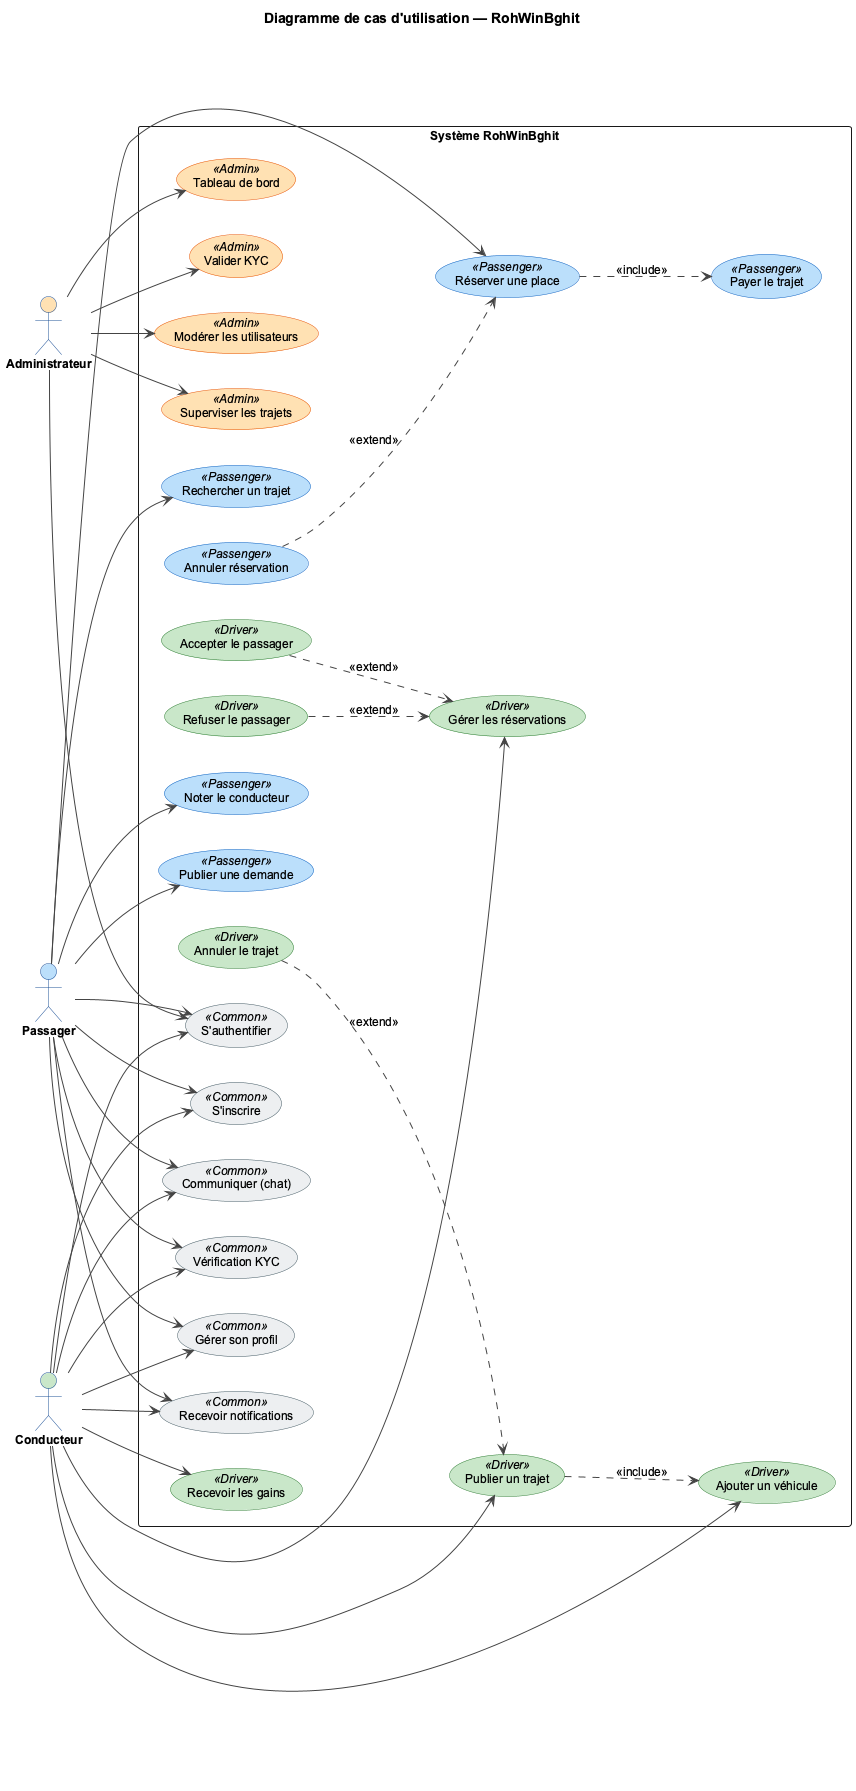
\includegraphics[width=0.95\linewidth,height=0.85\textheight,keepaspectratio]{fig_use_case.png}
\caption{Diagramme de cas d'utilisation consolidé (Passager, Conducteur, Administrateur)}
\label{fig:uc-global}
\end{figure}

Trois familles de cas se dégagent~: les cas \textit{transverses} (s'inscrire, se connecter par OTP, compléter le \textsc{kyc}, gérer son profil), les cas \textit{transactionnels} (publier, rechercher, réserver, payer) et les cas \textit{relationnels} (messagerie, notation, signalement). Les relations \texttt{include} traduisent les obligations métier (toute réservation passe par un paiement, toute connexion vérifie le statut \textsc{kyc}), tandis que les relations \texttt{extend} matérialisent les options (annulation, signalement).

Le tableau~\ref{tab:tracabilite} établit la \textbf{traçabilité} entre les besoins fonctionnels exprimés (section~\ref{sec:exigences-fonc}) et les cas d'utilisation principaux du système, garantissant qu'aucun besoin n'est laissé sans support.

\begin{table}[H]
\centering
\footnotesize
\begin{tabularx}{\textwidth}{|X|l|l|}
\hline
\rowcolor{rohlight}
\textbf{Besoin fonctionnel} & \textbf{Acteur} & \textbf{Cas d'utilisation} \\
\hline
Inscription / authentification OTP & Passager, Conducteur & UC-AUTH \\
\hline
Vérification d'identité biométrique & Passager, Conducteur & UC-KYC \\
\hline
Publication d'un trajet & Conducteur & UC-PUB-TRIP \\
\hline
Recherche d'un trajet & Passager & UC-SEARCH \\
\hline
Réservation et paiement & Passager & UC-BOOKING \\
\hline
Communication temps réel & Passager, Conducteur & UC-CHAT \\
\hline
Notation et avis & Passager, Conducteur & UC-REVIEW \\
\hline
Modération et validation \textsc{kyc} & Administrateur & UC-MODERATION \\
\hline
Tableau de bord et statistiques & Administrateur & UC-DASHBOARD \\
\hline
\end{tabularx}
  \caption{Matrice de traçabilité besoins fonctionnels $\leftrightarrow$ cas d'utilisation}
  \label{tab:tracabilite}
\end{table}

\section{Description textuelle des cas d'utilisation majeurs}
\label{sec:cu-textuel}

Les fiches descriptives ci-dessous formalisent les six cas d'utilisation les plus structurants. Elles suivent un canevas standard~: acteur principal, pré-conditions, scénario nominal, scénarios alternatifs, post-conditions.

\paragraph{UC-AUTH --- Inscription et authentification.}
\textit{Acteur~:} utilisateur non connecté.
\textit{Pré-conditions~:} disposer d'un numéro de téléphone algérien valide.
\textit{Scénario nominal~:} l'utilisateur saisit son numéro, reçoit un code OTP par \textsc{sms}, le valide, complète son profil minimal puis accède à la plateforme.
\textit{Alternatif~:} OTP expiré $\to$ renvoi possible toutes les 60~secondes.
\textit{Post-conditions~:} compte créé, jeton \gls{jwt} émis, statut \textsc{kyc} initialisé à \textit{unverified}.

\paragraph{UC-KYC --- Vérification d'identité biométrique.}
\textit{Acteur~:} utilisateur authentifié.
\textit{Pré-conditions~:} compte créé, statut \textit{unverified}.
\textit{Scénario nominal~:} téléversement du recto/verso de la carte d'identité, capture vidéo de vivacité (3~secondes), analyse asynchrone par le service IA, décision automatique (verified/pending\_review/rejected).
\textit{Alternatif~:} score intermédiaire $\to$ revue manuelle par l'administrateur.
\textit{Post-conditions~:} statut \textsc{kyc} mis à jour, \texttt{fraud\_event} consigné le cas échéant.

\paragraph{UC-PUB-TRIP --- Publication d'un trajet.}
\textit{Acteur~:} conducteur vérifié.
\textit{Scénario nominal~:} sélection des wilayas de départ et d'arrivée, choix du véhicule, date, heure, prix par place, nombre de places. Publication immédiate.
\textit{Post-conditions~:} trajet visible dans la recherche, indexé par couple (origine, destination, date).

\paragraph{UC-SEARCH --- Recherche d'un trajet.}
\textit{Acteur~:} passager.
\textit{Scénario nominal~:} saisie des wilayas et de la date, application des filtres (prix, nombre de places, note minimale), affichage des résultats triés.

\paragraph{UC-BOOKING --- Réservation et paiement.}
\textit{Acteur~:} passager vérifié.
\textit{Scénario nominal~:} sélection du trajet, choix du nombre de places, choix du moyen de paiement (\textsc{cib}, \textit{Edahabia}, espèces), exécution du paiement, confirmation de la réservation, notification au conducteur.
\textit{Alternatif~:} échec du paiement $\to$ remboursement automatique et notification au passager.

\paragraph{UC-MODERATION --- Modération et revue \textsc{kyc}.}
\textit{Acteur~:} administrateur.
\textit{Scénario nominal~:} consultation de la file d'attente \textit{pending\_review}, examen du dossier, validation ou rejet motivé, notification de l'utilisateur.

\section{Diagramme de classes détaillé}
\label{sec:classes}

Le diagramme de classes (figure~\ref{fig:classes}) représente la structure statique du domaine. Sa conception a été optimisée pour une projection directe vers un schéma relationnel \textsc{postgresql} normalisé en troisième forme normale.

\begin{figure}[H]
\centering
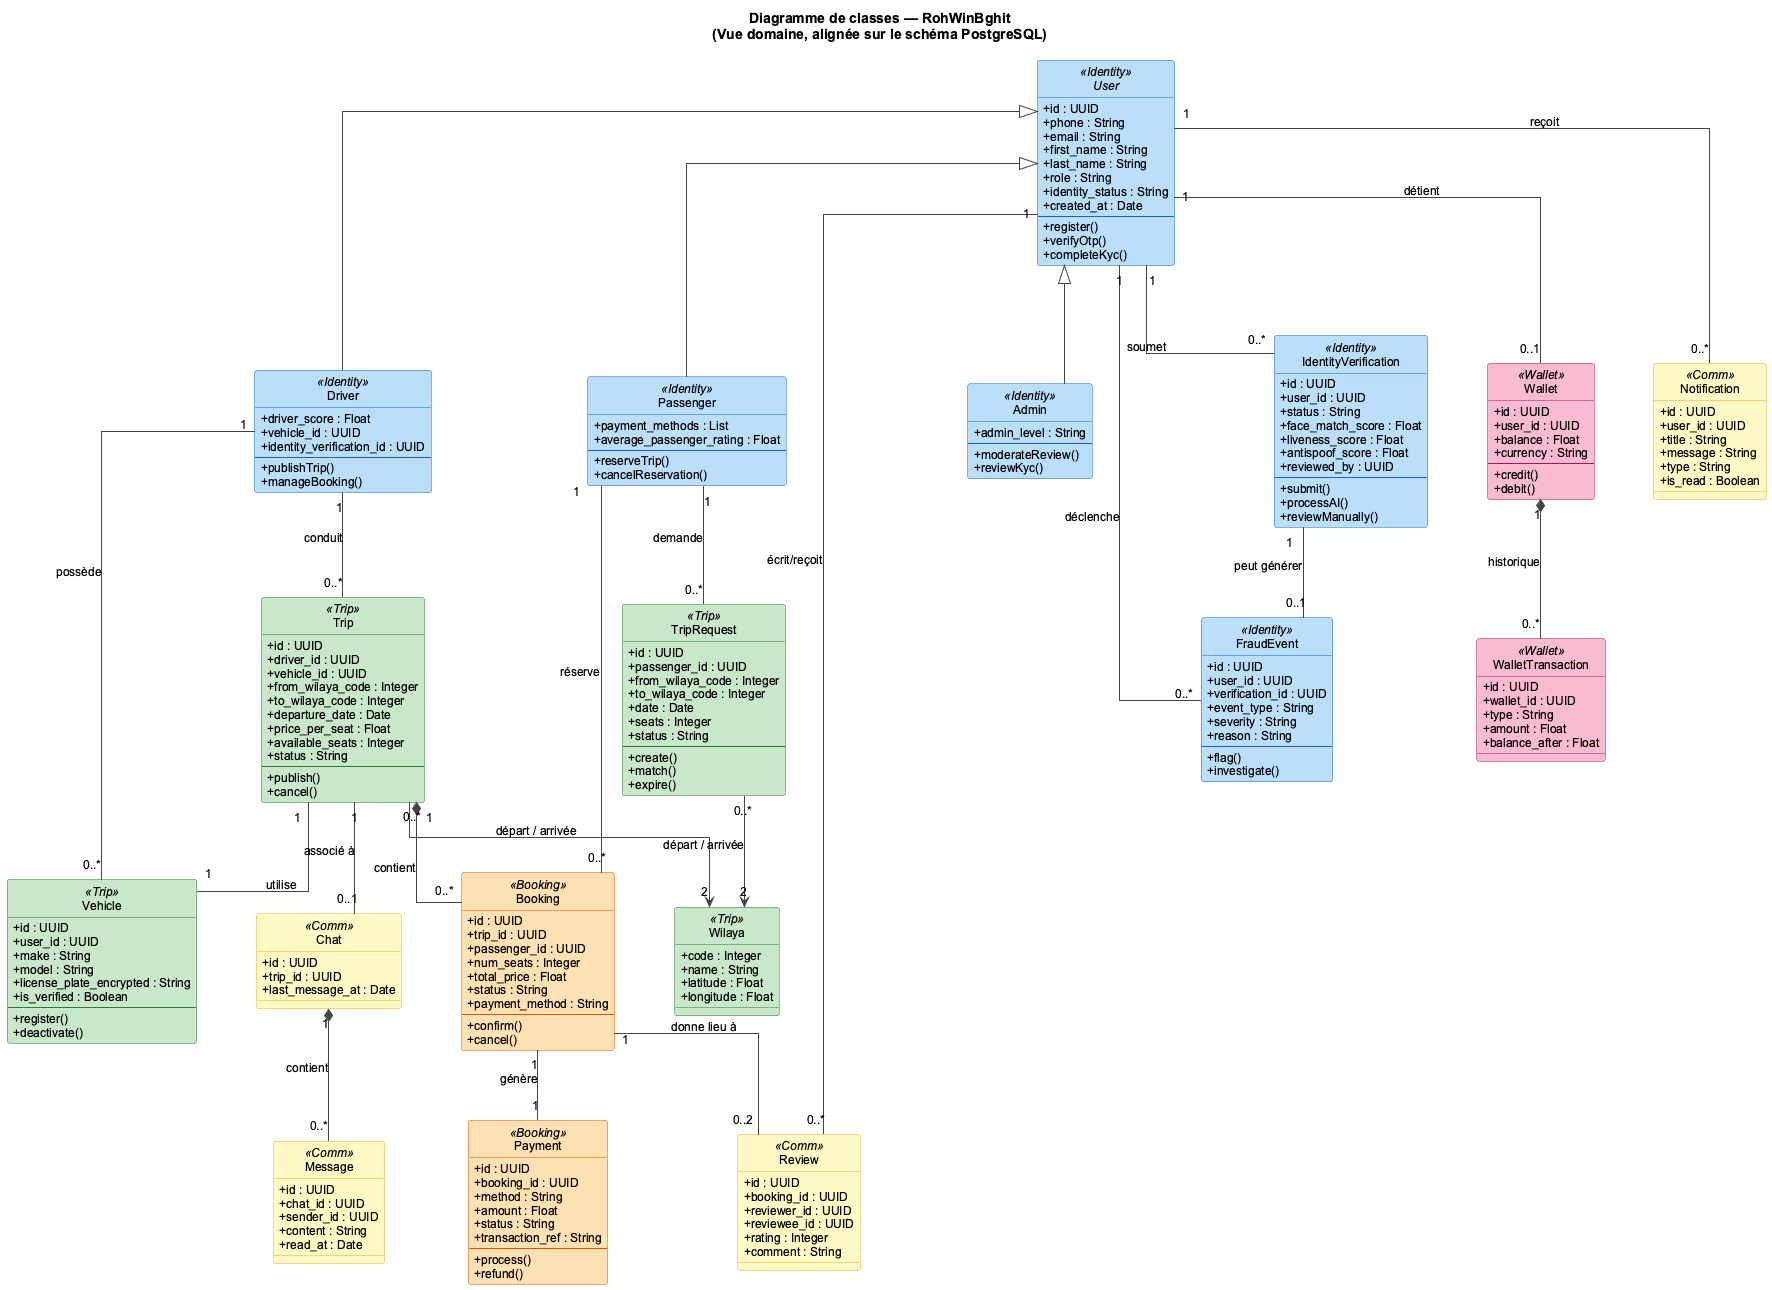
\includegraphics[width=\linewidth,height=0.85\textheight,keepaspectratio]{fig_class_diagram.png}
\caption{Diagramme de classes du domaine (alignement \textsc{postgresql})}
\label{fig:classes}
\end{figure}

Le modèle est organisé autour de la classe \texttt{User}, qui agrège les informations communes à tous les utilisateurs. La classe \texttt{Role} (passager, conducteur, administrateur) permet à un même utilisateur de cumuler plusieurs rôles via la table d'association \texttt{UserRole}. Le domaine s'articule autour de quatre agrégats~:
\begin{itemize}
  \item \textbf{Transport~:} \texttt{Trip}, \texttt{TripRequest}, \texttt{Route}, \texttt{Booking}, \texttt{Vehicle}.
  \item \textbf{Paiement~:} \texttt{Payment}, \texttt{Wallet}, \texttt{WalletTransaction}, \texttt{SurgePricingRule}.
  \item \textbf{Identité~:} \texttt{IdentityVerification}, \texttt{FaceEmbedding}, \texttt{FraudEvent}.
  \item \textbf{Communication~:} \texttt{Chat}, \texttt{Message}, \texttt{Notification}, \texttt{Review}.
\end{itemize}

\subsection{Description des classes}

Le tableau~\ref{tab:classes} synthétise les dix-sept classes principales, leurs attributs et leurs méthodes métier clés.

\begin{table}[H]
\centering
\footnotesize
\begin{tabularx}{\textwidth}{|l|X|X|}
\hline
\rowcolor{rohlight}
\textbf{Classe} & \textbf{Attributs principaux} & \textbf{Méthodes métier} \\
\hline
\texttt{User} & id, phone, email, firstName, lastName, dateOfBirth, verificationStatus, createdAt & register(), verifyOtp(), completeKyc(), updateProfile() \\
\hline
\texttt{Role} & id, name, permissions & hasPermission(), assignToUser() \\
\hline
\texttt{Vehicle} & id, driverId, brand, model, licensePlate, color, seatsAvailable & register(), update(), deactivate() \\
\hline
\texttt{Trip} & id, driverId, vehicleId, originWilayaId, destinationWilayaId, departureAt, pricePerSeat, availableSeats, status & publish(), cancel(), computeSurgePrice() \\
\hline
\texttt{TripRequest} & id, passengerId, fromWilayaCode, toWilayaCode, requestedDate, seats, status, expiresAt & create(), match(), expire() \\
\hline
\texttt{Route} & id, driverId, fromWilayaCode, toWilayaCode, isHabitual, frequency & register(), computeDistance() \\
\hline
\texttt{Booking} & id, tripId, passengerId, seats, totalPrice, status, paymentStatus, createdAt & confirm(), cancel(), generateQr() \\
\hline
\texttt{Payment} & id, bookingId, method, amount, status, transactionRef & process(), refund(), getReceipt() \\
\hline
\texttt{IdentityVerification} & id, userId, idFrontUrl, idBackUrl, videoUrl, faceMatchScore, livenessScore, antispoofScore, aiScore, status, role & submit(), processAI(), reviewManually() \\
\hline
\texttt{FraudEvent} & id, userId, verificationId, eventType, severity, reason, aiScores & flag(), investigate() \\
\hline
\texttt{FaceEmbedding} & id, userId, embedding, version, createdAt & generate(), compare() \\
\hline
\texttt{Wallet} & id, userId, balance, currency & credit(), debit(), withdraw() \\
\hline
\texttt{WalletTransaction} & id, walletId, type, amount, reference, createdAt & record(), reverse() \\
\hline
\texttt{Review} & id, tripId, authorId, targetId, rating, comment, createdAt & submit(), moderate() \\
\hline
\texttt{Chat / Message} & id, tripId, senderId, content, sentAt, readAt & send(), markAsRead() \\
\hline
\texttt{Notification} & id, userId, type, title, body, data, readAt & dispatch(), markAsRead() \\
\hline
\texttt{SurgePricingRule} & id, wilayaCode, dayOfWeek, hourStart, hourEnd, multiplier, isActive & evaluate(), cache() \\
\hline
\end{tabularx}
  \caption{Description des classes du domaine}
  \label{tab:classes}
\end{table}

\subsection{Dictionnaire de données des entités critiques}

Pour les entités les plus structurantes, nous précisons le type \textsc{postgresql} et les contraintes (tableaux~\ref{tab:dict-user}, \ref{tab:dict-trip}, \ref{tab:dict-booking}, \ref{tab:dict-kyc}).

\begin{table}[H]
\centering
\footnotesize
\begin{tabularx}{\textwidth}{|l|l|X|}
\hline
\rowcolor{rohlight}
\textbf{Attribut} & \textbf{Type \textsc{postgresql}} & \textbf{Description / contraintes} \\
\hline
id & UUID & Clé primaire (v4) \\
\hline
phone & VARCHAR(20) & Format E.164, UNIQUE, NOT NULL \\
\hline
email & VARCHAR(100) & UNIQUE, NULLABLE \\
\hline
firstName & VARCHAR(50) & NOT NULL \\
\hline
lastName & VARCHAR(50) & NOT NULL \\
\hline
passwordHash & VARCHAR(255) & NOT NULL (bcrypt) \\
\hline
verificationStatus & VARCHAR(20) & ENUM, défaut \textit{unverified} \\
\hline
createdAt & TIMESTAMPTZ & DEFAULT NOW() \\
\hline
\end{tabularx}
  \caption{Dictionnaire de données --- entité \texttt{User}}
  \label{tab:dict-user}
\end{table}

\begin{table}[H]
\centering
\footnotesize
\begin{tabularx}{\textwidth}{|l|l|X|}
\hline
\rowcolor{rohlight}
\textbf{Attribut} & \textbf{Type} & \textbf{Description / contraintes} \\
\hline
id & UUID & Clé primaire \\
\hline
driverId & UUID & FK \texttt{users.id}, NOT NULL \\
\hline
vehicleId & UUID & FK \texttt{vehicles.id}, NOT NULL \\
\hline
originWilayaId & INTEGER & FK \texttt{wilayas.id}, NOT NULL \\
\hline
destinationWilayaId & INTEGER & FK \texttt{wilayas.id}, NOT NULL \\
\hline
departureAt & TIMESTAMPTZ & NOT NULL, $>$ NOW() \\
\hline
pricePerSeat & DECIMAL(10,2) & NOT NULL, $>$ 0 \\
\hline
availableSeats & INTEGER & NOT NULL, dans [0, capacité] \\
\hline
status & VARCHAR(20) & ENUM (\textit{scheduled / in\_progress / completed / cancelled}) \\
\hline
\end{tabularx}
  \caption{Dictionnaire de données --- entité \texttt{Trip}}
  \label{tab:dict-trip}
\end{table}

\begin{table}[H]
\centering
\footnotesize
\begin{tabularx}{\textwidth}{|l|l|X|}
\hline
\rowcolor{rohlight}
\textbf{Attribut} & \textbf{Type} & \textbf{Description / contraintes} \\
\hline
id & UUID & Clé primaire \\
\hline
tripId & UUID & FK \texttt{trips.id}, NOT NULL \\
\hline
passengerId & UUID & FK \texttt{users.id}, NOT NULL \\
\hline
seats & INTEGER & NOT NULL, $>$ 0 \\
\hline
totalPrice & DECIMAL(10,2) & seats $\times$ pricePerSeat, NOT NULL \\
\hline
status & VARCHAR(20) & ENUM (\textit{pending / confirmed / cancelled / completed}) \\
\hline
paymentStatus & VARCHAR(20) & ENUM (\textit{pending / paid / refunded / failed}) \\
\hline
\end{tabularx}
  \caption{Dictionnaire de données --- entité \texttt{Booking}}
  \label{tab:dict-booking}
\end{table}

\begin{table}[H]
\centering
\footnotesize
\begin{tabularx}{\textwidth}{|l|l|X|}
\hline
\rowcolor{rohlight}
\textbf{Attribut} & \textbf{Type} & \textbf{Description / contraintes} \\
\hline
id & UUID & Clé primaire \\
\hline
userId & UUID & FK \texttt{users.id}, UNIQUE par rôle \\
\hline
idFrontUrl & VARCHAR(255) & Cloudinary, chiffré au repos \\
\hline
idBackUrl & VARCHAR(255) & Cloudinary \\
\hline
faceMatchScore & DECIMAL(5,4) & Similarité InsightFace [0,1] \\
\hline
livenessScore & DECIMAL(5,4) & Détection de vivacité [0,1] \\
\hline
status & VARCHAR(20) & ENUM (\textit{pending / verified / rejected / manual\_review}) \\
\hline
role & VARCHAR(20) & \textit{driver} ou \textit{passenger} \\
\hline
\end{tabularx}
  \caption{Dictionnaire de données --- entité \texttt{IdentityVerification} (\textsc{kyc})}
  \label{tab:dict-kyc}
\end{table}

\subsection{Modèle relationnel synthétique}

Le passage du diagramme de classes au schéma relationnel suit les règles classiques de transformation. Les principales relations sont représentées ci-dessous (les clés primaires sont soulignées, les clés étrangères préfixées par~\#).

\begin{highlight}
\small
\texttt{User}(\underline{id}, phone, email, firstName, lastName, dateOfBirth, passwordHash, verificationStatus, identityVerifiedAt, createdAt)\\[2pt]
\texttt{Role}(\underline{id}, name, permissions)\\[2pt]
\texttt{UserRole}(\underline{\#userId}, \underline{\#roleId})\\[2pt]
\texttt{Vehicle}(\underline{id}, \#driverId, brand, model, licensePlate, color, seatsAvailable, isActive)\\[2pt]
\texttt{Wilaya}(\underline{id}, code, nameFr, nameAr, latitude, longitude)\\[2pt]
\texttt{Route}(\underline{id}, \#driverId, \#fromWilayaCode, \#toWilayaCode, isHabitual, frequency)\\[2pt]
\texttt{Trip}(\underline{id}, \#driverId, \#vehicleId, \#originWilayaId, \#destinationWilayaId, departureAt, pricePerSeat, availableSeats, status, createdAt)\\[2pt]
\texttt{TripRequest}(\underline{id}, \#passengerId, \#fromWilayaCode, \#toWilayaCode, requestedDate, seats, status, expiresAt, createdAt)\\[2pt]
\texttt{Booking}(\underline{id}, \#tripId, \#passengerId, seats, totalPrice, status, paymentStatus, createdAt)\\[2pt]
\texttt{Payment}(\underline{id}, \#bookingId, method, amount, status, transactionRef, createdAt)\\[2pt]
\texttt{IdentityVerification}(\underline{id}, \#userId, idFrontUrl, idBackUrl, videoUrl, faceMatchScore, livenessScore, antispoofScore, aiScore, status, role, reviewedBy, reviewedAt)\\[2pt]
\texttt{FraudEvent}(\underline{id}, \#userId, \#verificationId, eventType, severity, reason, aiScores, createdAt)\\[2pt]
\texttt{FaceEmbedding}(\underline{id}, \#userId, embedding, version, createdAt)\\[2pt]
\texttt{SurgePricingRule}(\underline{id}, wilayaCode, dayOfWeek, hourStart, hourEnd, multiplier, isActive)\\[2pt]
\texttt{Wallet}(\underline{id}, \#userId, balance, currency)\\[2pt]
\texttt{WalletTransaction}(\underline{id}, \#walletId, type, amount, reference, createdAt)\\[2pt]
\texttt{Chat}(\underline{id}, \#tripId, createdAt)\\[2pt]
\texttt{Message}(\underline{id}, \#chatId, \#senderId, content, sentAt, readAt)\\[2pt]
\texttt{Notification}(\underline{id}, \#userId, type, title, body, data, readAt, createdAt)\\[2pt]
\texttt{Review}(\underline{id}, \#tripId, \#authorId, \#targetId, rating, comment, createdAt)
\end{highlight}

\section{Diagrammes de séquence essentiels}
\label{sec:sequences}

Sept scénarios couvrent l'essentiel de la complexité dynamique du système. Quatre d'entre eux suivent le parcours utilisateur classique (inscription, authentification, réservation côté passager, réservation côté conducteur)~; trois sont propres aux apports techniques de \textit{RohWinBghit} (paiement multi-méthodes, vérification \textsc{kyc} biométrique, demande de trajet en \textit{matching} inverse).

\subsection{Inscription}

L'inscription (figure~\ref{fig:seq-inscription}) repose sur une vérification du numéro de téléphone par code OTP envoyé par \textsc{sms}, suivie de la saisie des informations personnelles et de l'attribution du rôle (passager ou conducteur).

\begin{figure}[H]
\centering
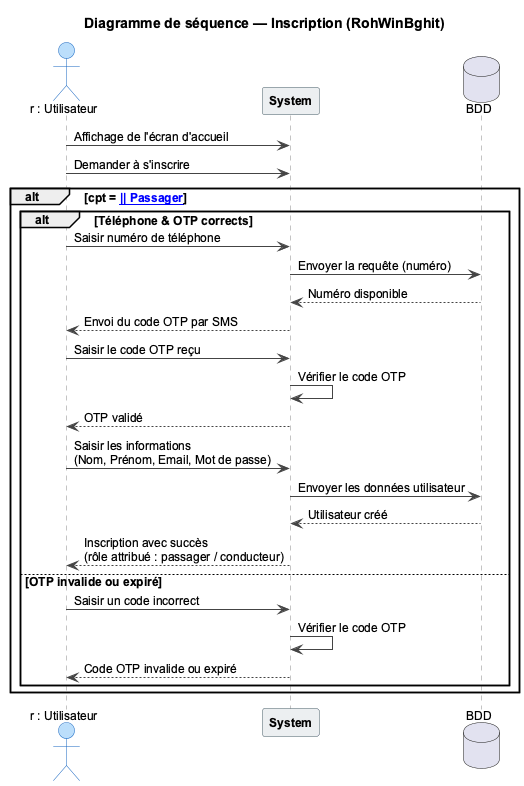
\includegraphics[width=0.85\linewidth]{fig_sequence_inscription.png}
\caption{Séquence --- Inscription d'un nouvel utilisateur}
\label{fig:seq-inscription}
\end{figure}

Le flux distingue explicitement les cas d'OTP valide et invalide, et déclenche en fin de parcours la création de l'utilisateur en base avec un statut \textsc{kyc} initialisé à \textit{unverified}.

\subsection{Authentification}

L'authentification (figure~\ref{fig:seq-authentification}) emprunte le même mécanisme OTP. Une fois validée, elle bifurque selon le rôle pour orienter l'utilisateur vers les actions disponibles~: recherche et réservation de covoiturage côté passager~; gestion des véhicules, publication de trajet et suivi des demandes côté conducteur.

\begin{figure}[H]
\centering
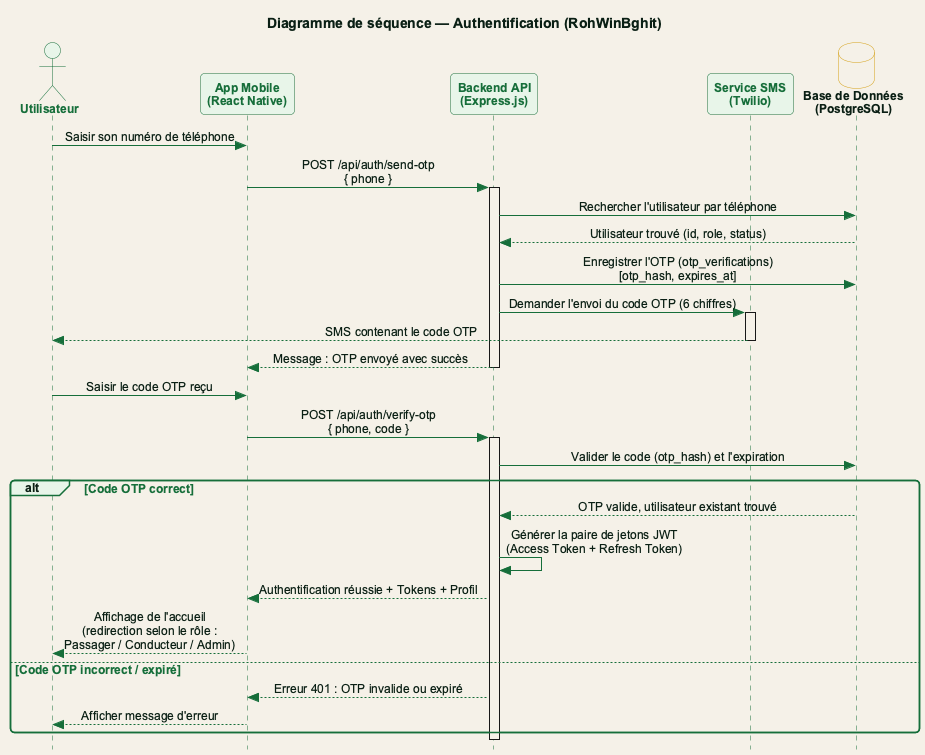
\includegraphics[width=0.95\linewidth]{fig_sequence_authentification.png}
\caption{Séquence --- Authentification et orientation par rôle}
\label{fig:seq-authentification}
\end{figure}

\subsection{Réservation côté passager}

Le scénario de réservation côté passager (figure~\ref{fig:seq-reservation-passager}) couvre la recherche d'un covoiturage, l'affichage des détails, la réservation avec choix du moyen de paiement, puis trois issues possibles selon la décision du conducteur~: acceptation (suivie de la fin du trajet et de la notation), refus (notification au passager) ou annulation à l'initiative du passager.

\begin{figure}[H]
\centering
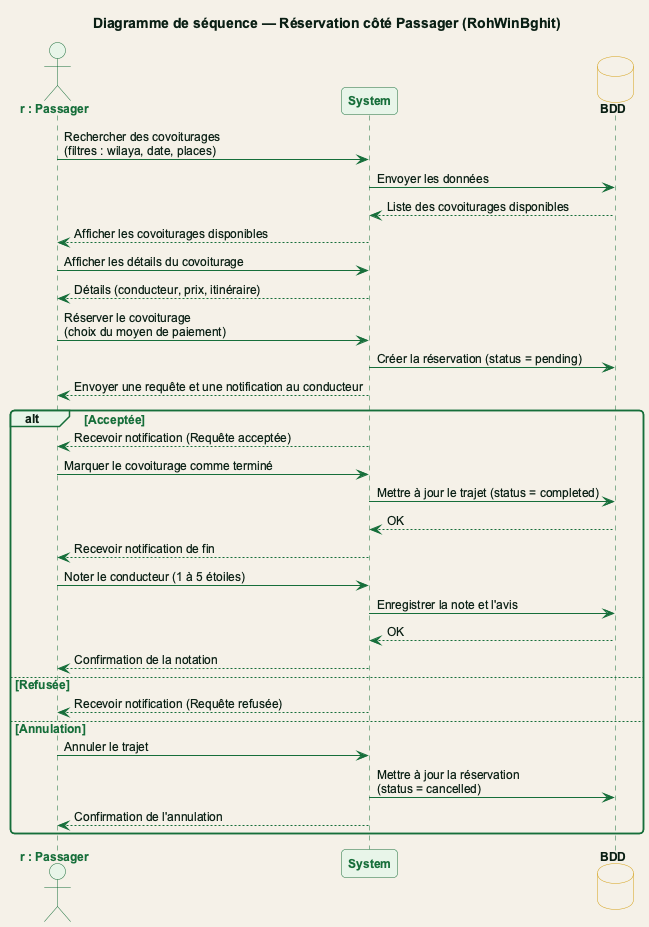
\includegraphics[width=0.95\linewidth]{fig_sequence_reservation_passager.png}
\caption{Séquence --- Réservation côté passager}
\label{fig:seq-reservation-passager}
\end{figure}

\subsection{Réservation côté conducteur}

Le pendant côté conducteur (figure~\ref{fig:seq-reservation-conducteur}) modélise la réception des notifications de demande, l'accès à la gestion des covoiturages, et les trois décisions possibles~: accepter le passager (mise à jour de la réservation et notification), refuser (rejet et notification), ou annuler le trajet (mise à jour du statut et alerte des passagers concernés).

\begin{figure}[H]
\centering
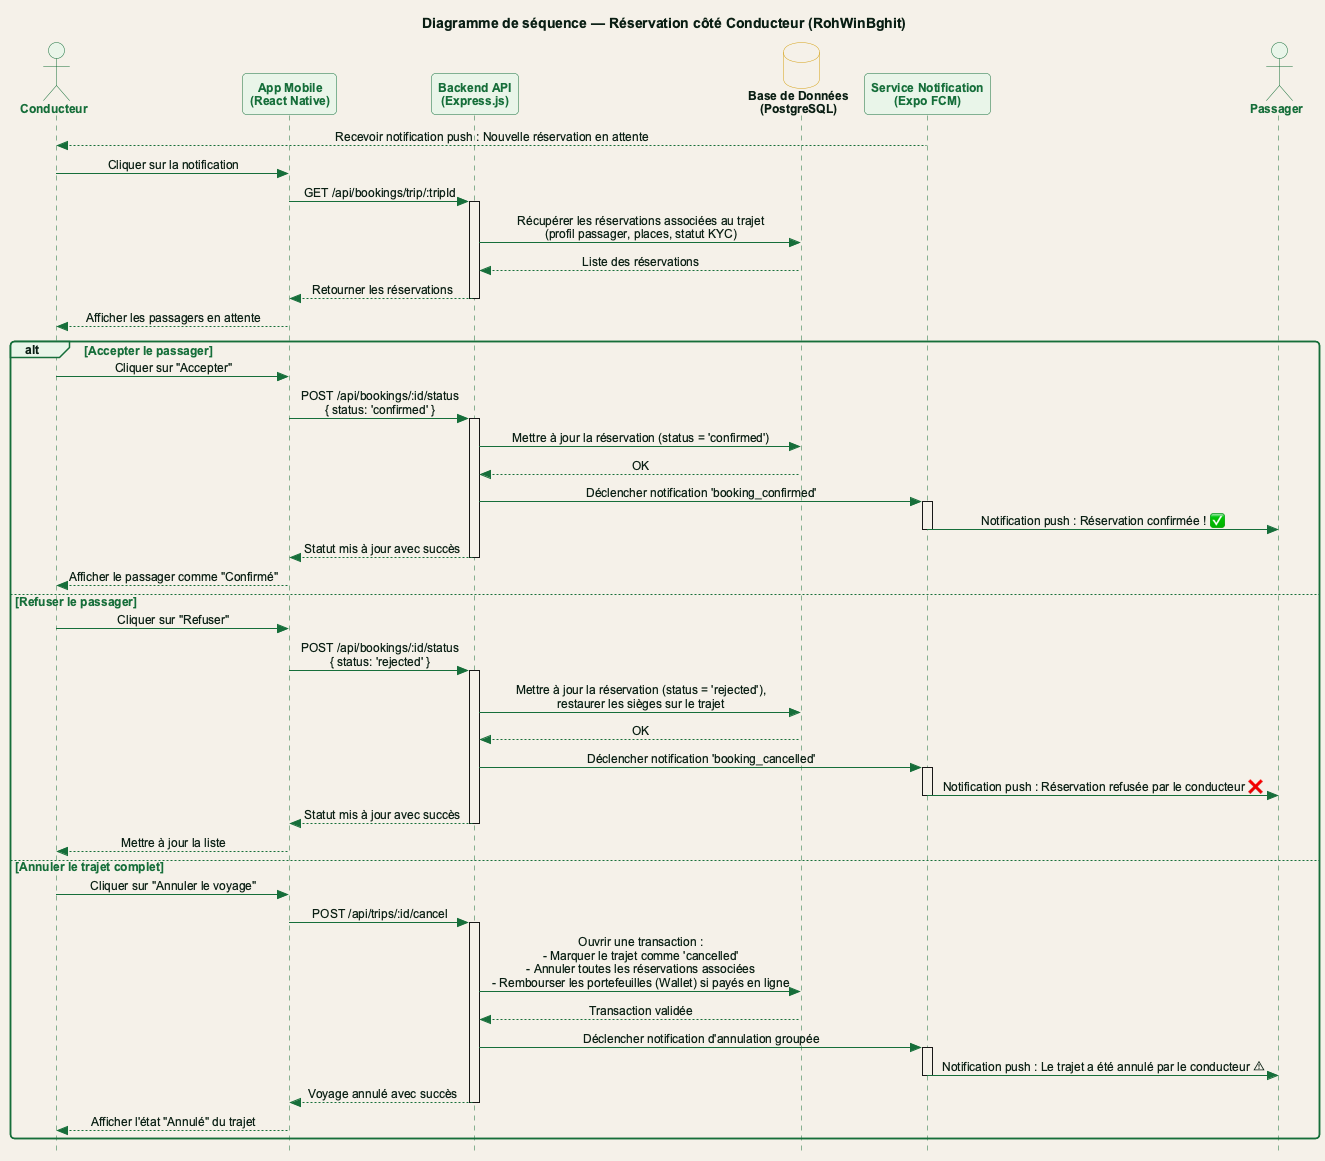
\includegraphics[width=0.95\linewidth]{fig_sequence_reservation_conducteur.png}
\caption{Séquence --- Réservation côté conducteur}
\label{fig:seq-reservation-conducteur}
\end{figure}

\subsection{Réservation avec paiement multi-méthodes (vue technique)}

La figure~\ref{fig:seq-reservation} approfondit la séquence de réservation en exposant l'orchestration interne du paiement~: vérification de la disponibilité, calcul du tarif dynamique par le \texttt{FareService} (avec multiplicateur de \textit{surge pricing} mis en cache dans Redis), exécution du paiement via le patron \textit{Strategy/Factory} (\texttt{PaymentFactory} résolvant la stratégie \textsc{cib}, \textit{Edahabia} ou espèces), persistance transactionnelle en \textsc{postgresql} et notification \textit{push} au conducteur.

\begin{figure}[H]
\centering
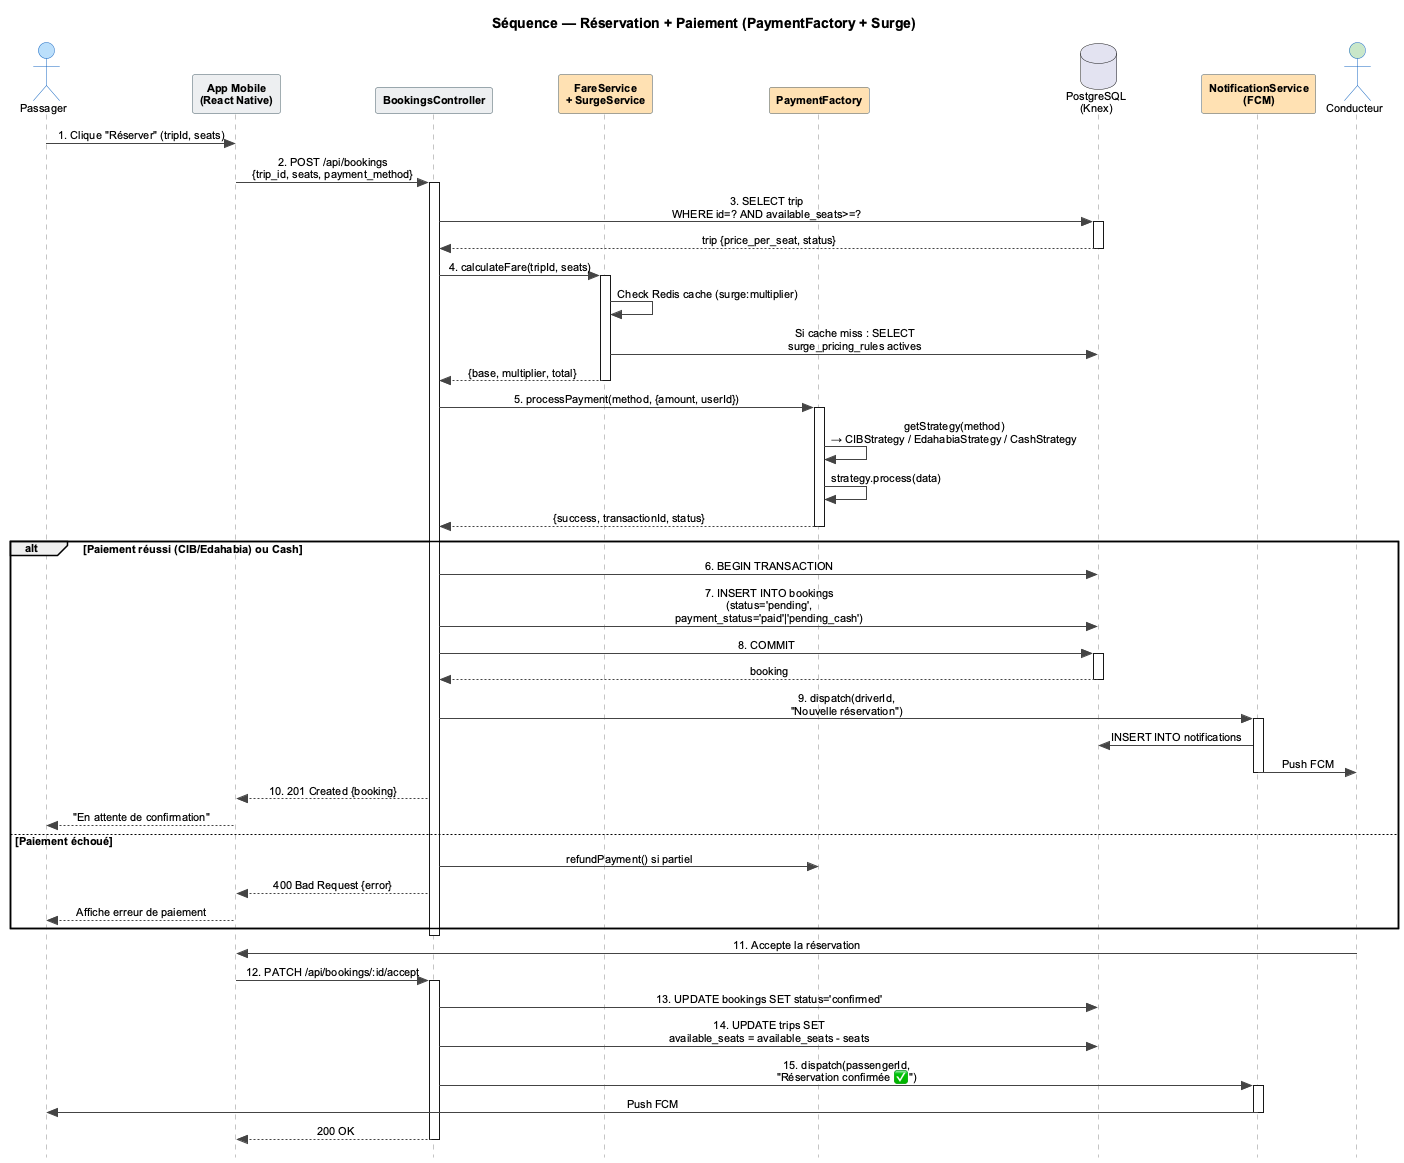
\includegraphics[width=0.95\linewidth]{fig_sequence_booking.png}
\caption{Séquence --- Réservation avec paiement multi-méthodes (vue technique)}
\label{fig:seq-reservation}
\end{figure}

Le bloc \texttt{alt} illustre les deux issues possibles~: succès (ou paiement en espèces) entraînant la persistance et la notification \textsc{fcm}~; échec déclenchant un remboursement et une notification au passager.

\subsection{Vérification \textsc{kyc} biométrique}

Le flux \textsc{kyc} (figure~\ref{fig:seq-kyc}) constitue le scénario le plus critique en termes de sécurité. Cinq étapes le structurent~: téléversement du document, capture vidéo de vivacité, traitement asynchrone par le pipeline IA (comparaison faciale InsightFace, détection de vivacité, anti-\textit{spoofing}), décision automatique à trois états (\textit{verified}, \textit{pending\_review}, \textit{rejected}), et éventuelle revue manuelle.

\begin{figure}[H]
\centering
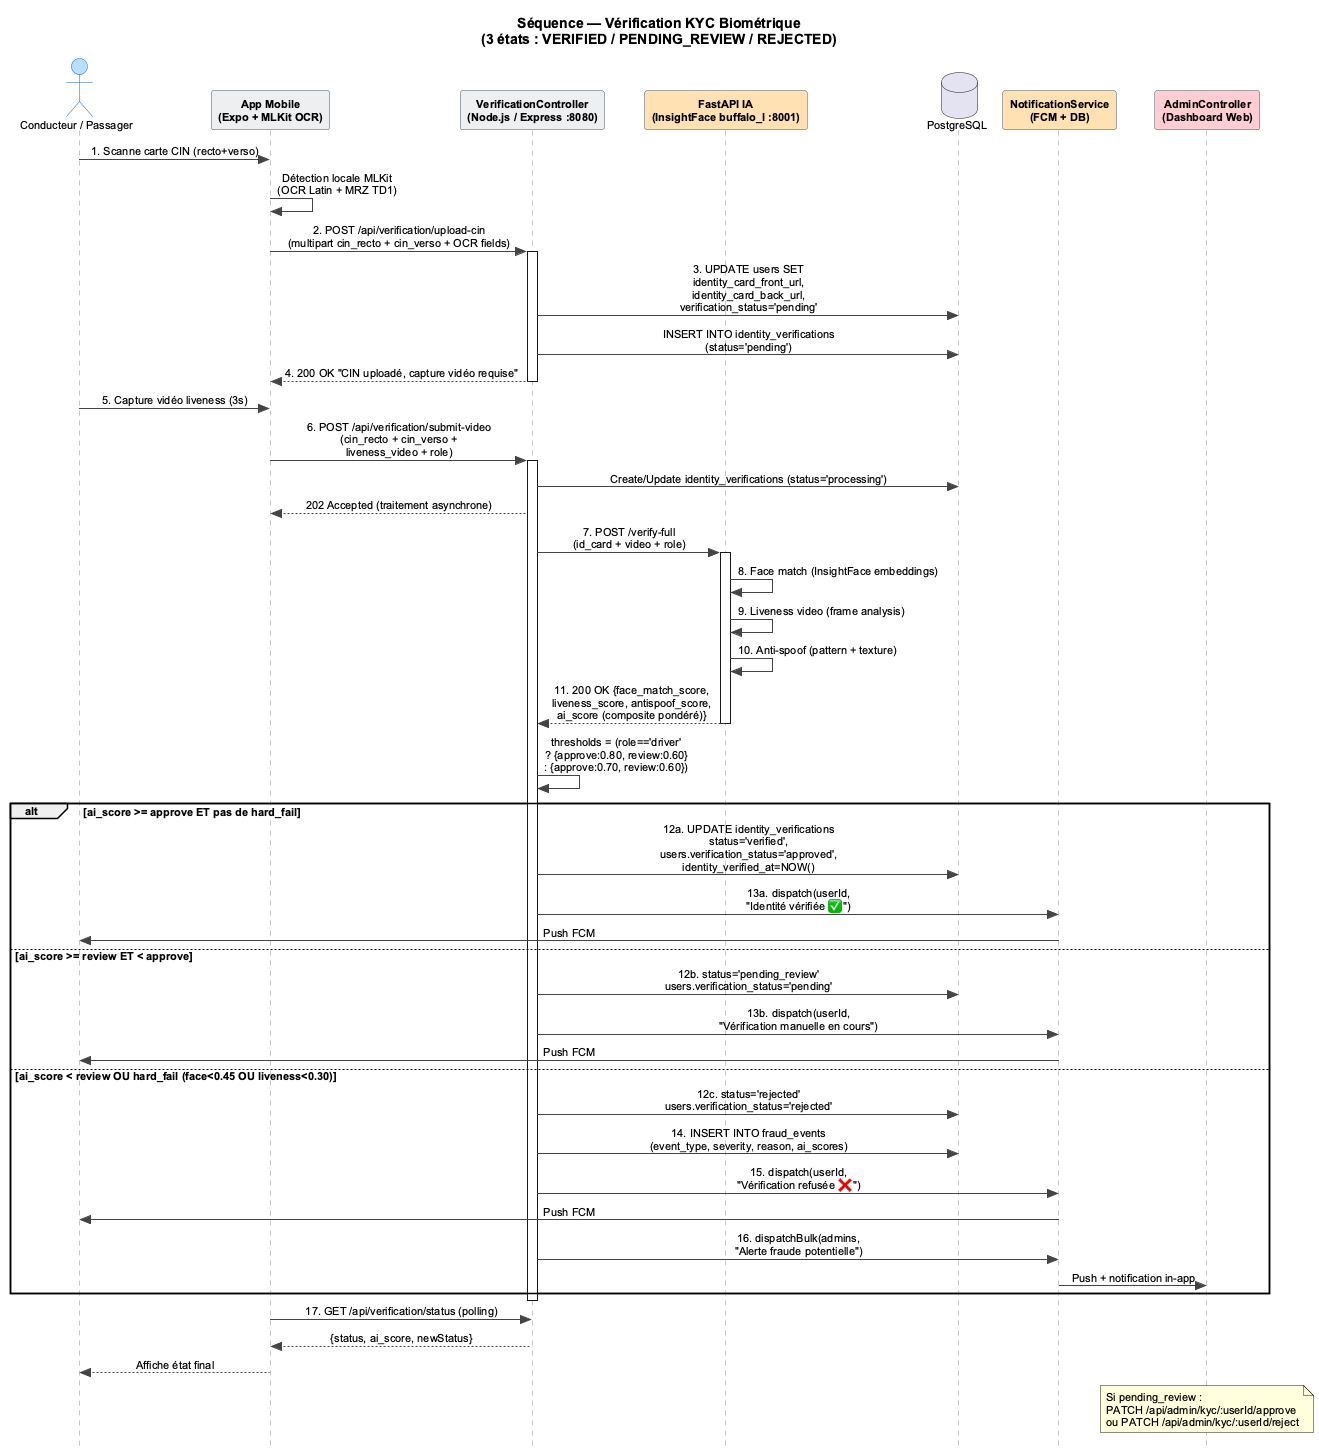
\includegraphics[width=0.95\linewidth]{fig_sequence_kyc.png}
\caption{Séquence --- Vérification \textsc{kyc} biométrique (3~états de décision)}
\label{fig:seq-kyc}
\end{figure}

Les seuils retenus sont différenciés par rôle, en réponse aux contraintes opérationnelles spécifiques. Pour un conducteur, on requiert un score facial $\geq$~0{,}65, un score de vivacité $\geq$~0{,}65 et un score anti-\textit{spoofing} $\geq$~0{,}60~; pour un passager, les seuils correspondants sont de 0{,}60, 0{,}55 et 0{,}50. Un \textit{hard-fail} (rejet automatique avec consignation d'un \texttt{fraud\_event}) est déclenché en cas de score très bas. Les cas intermédiaires sont placés en file d'attente pour revue manuelle.

\subsection{Demande de trajet (\textit{matching} inverse)}

La figure~\ref{fig:seq-trip-request} modélise le scénario inverse de la publication classique~: le passager exprime une demande, et le système identifie les conducteurs éligibles.

\begin{figure}[H]
\centering
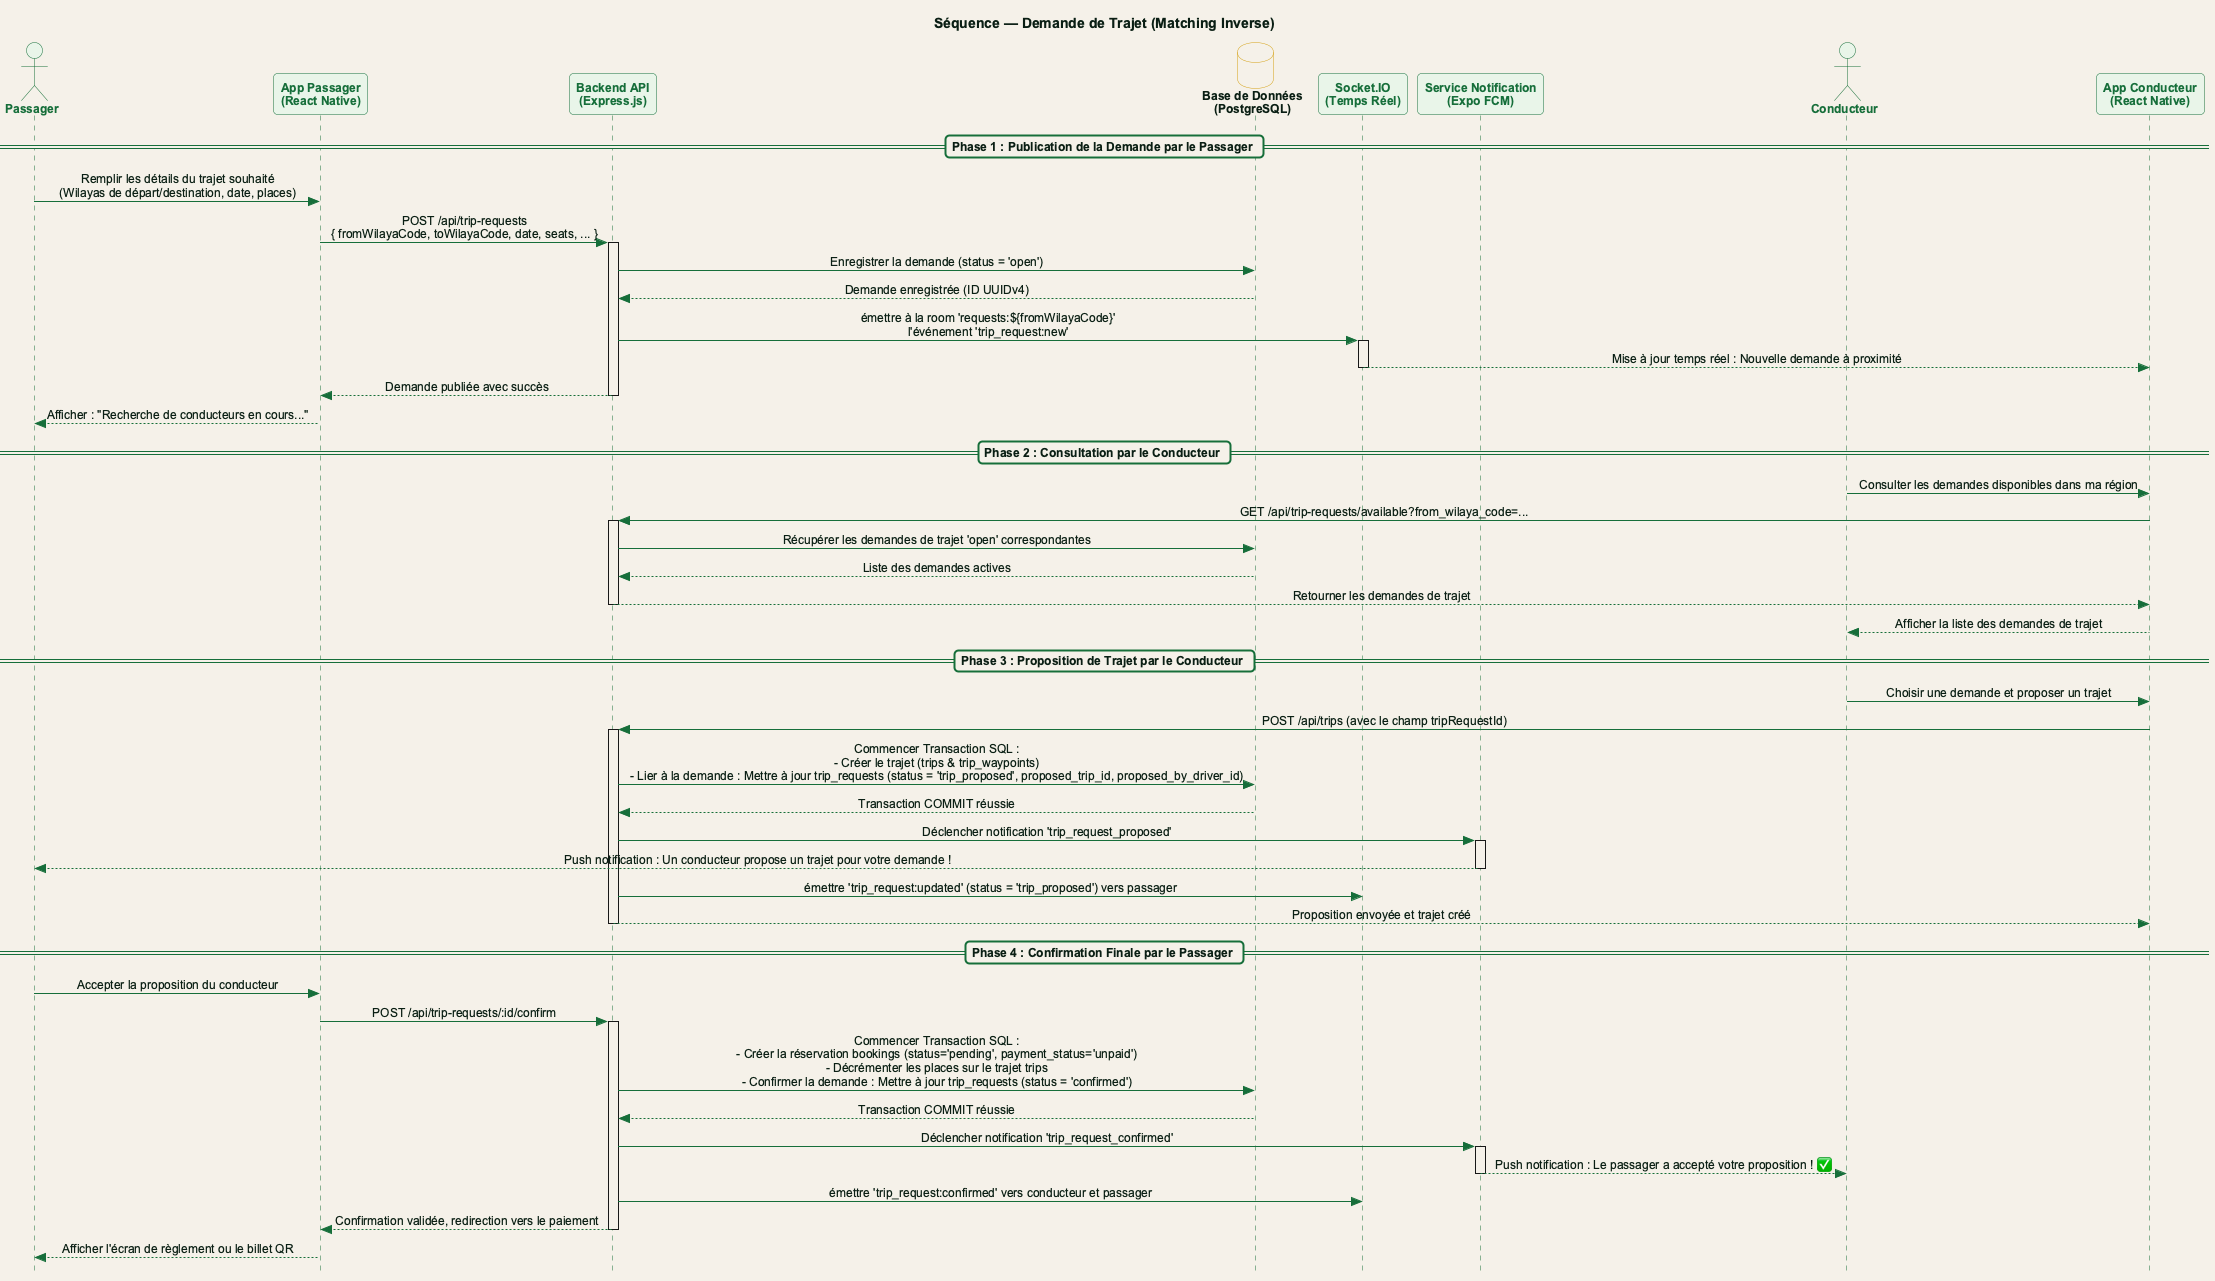
\includegraphics[width=0.95\linewidth]{fig_sequence_trip_request.png}
\caption{Séquence --- Demande de trajet (\textit{matching} passager $\to$ conducteurs)}
\label{fig:seq-trip-request}
\end{figure}

Cinq phases structurent le flux~: soumission de la demande avec délai d'expiration de 24~heures, interrogation de la base par le \texttt{MatchingService}, diffusion des notifications \textit{push} aux conducteurs éligibles, réception de la première proposition compatible, transition de la demande vers le statut \textit{matched}.

\section{Diagramme d'activité principal}
\label{sec:activite}

Le diagramme d'activité de la figure~\ref{fig:activite-booking} décrit, du point de vue procédural, le \textbf{parcours global d'un utilisateur} sur la plateforme, depuis l'authentification jusqu'à la fin du trajet. Il complète les diagrammes de séquence en exposant la totalité des branchements et des boucles sous une forme synthétique.

\begin{figure}[H]
\centering
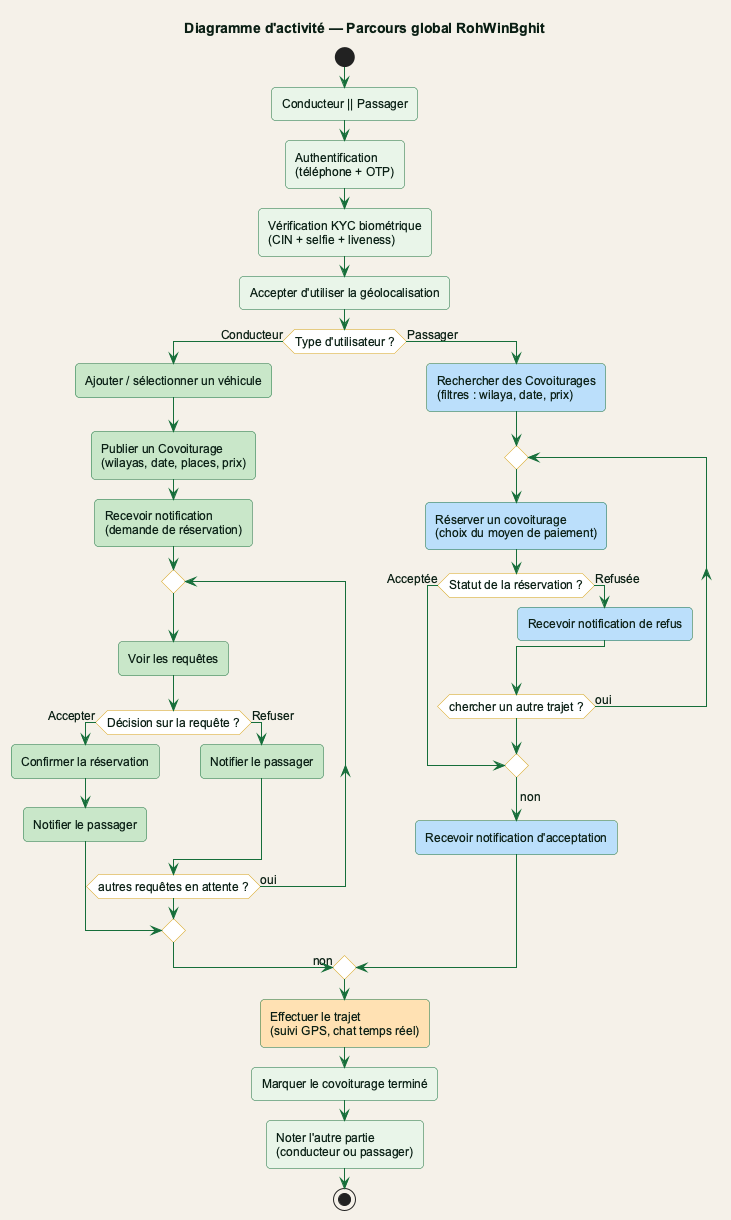
\includegraphics[width=0.85\linewidth,height=0.85\textheight,keepaspectratio]{fig_activity_main.png}
\caption{Diagramme d'activité --- parcours global de la plateforme}
\label{fig:activite-booking}
\end{figure}

Après authentification et vérification \textsc{kyc} biométrique, l'utilisateur est orienté vers l'une des deux branches selon son rôle. \textbf{Côté conducteur}, il déclare un véhicule, publie un covoiturage, reçoit les demandes de réservation et décide pour chacune (accepter ou refuser) en boucle jusqu'à épuisement de la file. \textbf{Côté passager}, il recherche un trajet, soumet une réservation et attend la décision du conducteur~; en cas de refus, il peut relancer une recherche. Le flux converge en fin de parcours sur le trajet effectif (suivi GPS, chat temps réel), la clôture du covoiturage et la notation mutuelle. Trois branches mènent respectivement à l'exécution \textsc{cib}, \textit{Edahabia} ou en espèces. Les nœuds de décision matérialisent les ruptures possibles (places insuffisantes, paiement échoué, conducteur ne confirmant pas dans le délai), chacune associée à un message d'erreur explicite et à une compensation (libération de places, remboursement, file d'attente).

\section{Architecture logique de la solution}
\label{sec:architecture}

L'architecture cible suit un découpage \textbf{multi-services} où chaque composant communique via des interfaces explicitement définies (figure~\ref{fig:archi-globale}).

\begin{figure}[H]
\centering
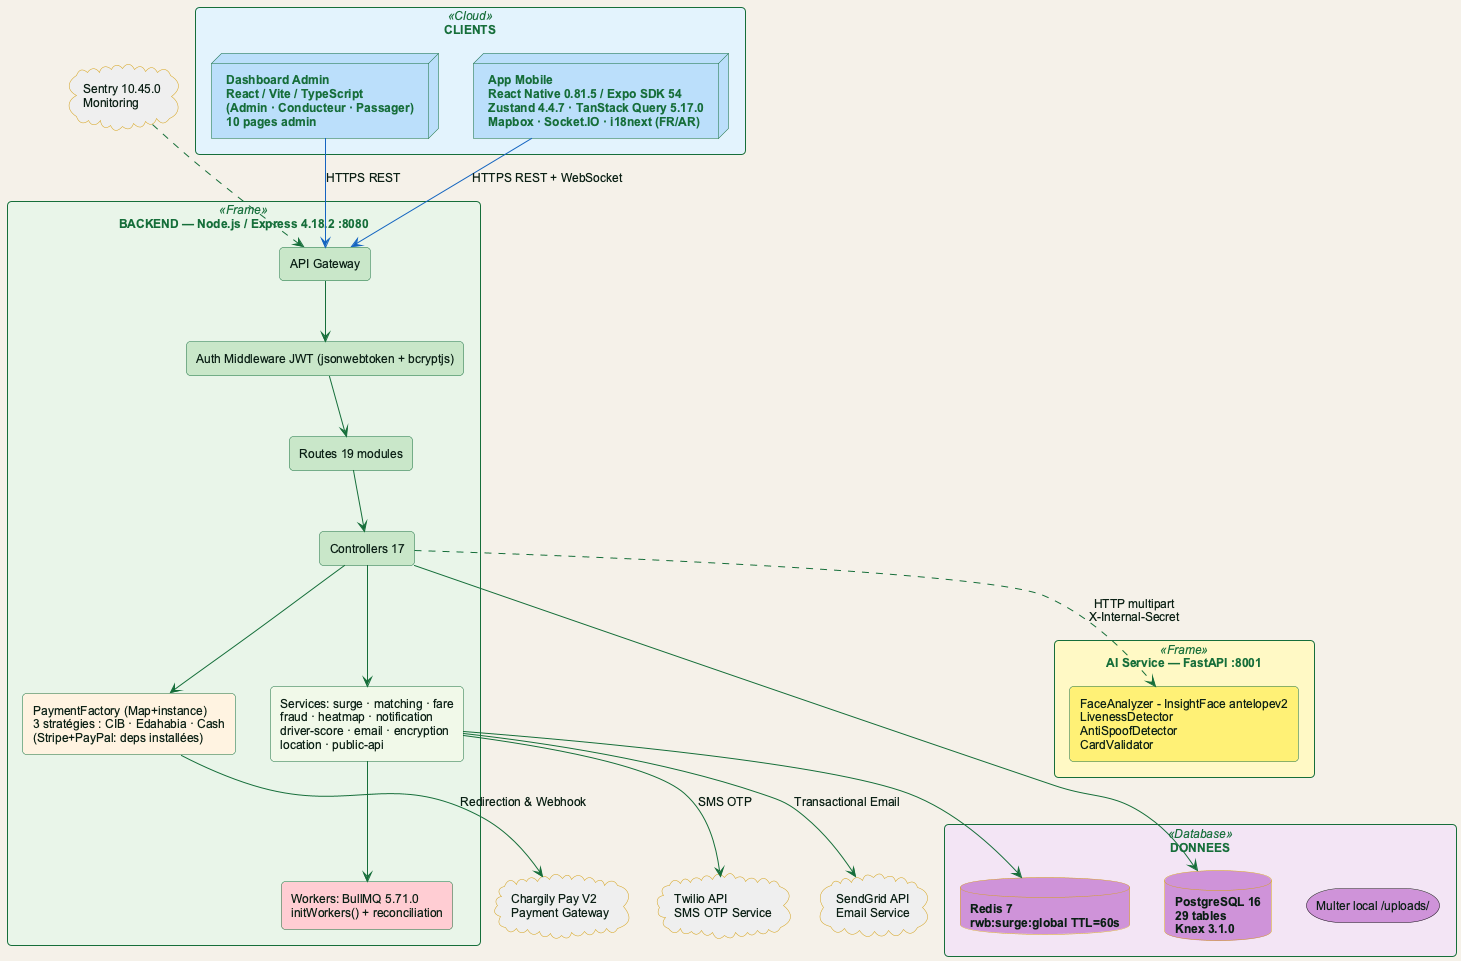
\includegraphics[width=0.95\linewidth]{fig_architecture.png}
\caption{Architecture globale de \textit{RohWinBghit}}
\label{fig:archi-globale}
\end{figure}

\begin{itemize}
  \item \textbf{Application mobile} (React~Native, Expo, TypeScript) --- interface principale conducteur/passager.
  \item \textbf{Tableau de bord administrateur} (Next.js / React) --- modération, validation \textsc{kyc}, statistiques.
  \item \textbf{Back-end API} (NestJS / Node.js) --- logique métier, authentification, persistance, communication temps réel.
  \item \textbf{Service IA} (FastAPI / Python) --- traitement biométrique \textsc{kyc} (OCR, comparaison faciale, vivacité, anti-\textit{spoofing}).
  \item \textbf{Base de données} (\textsc{postgresql}) et \textbf{cache} (Redis).
  \item \textbf{Notifications push} via Firebase \textsc{fcm}~; cartographie via Mapbox~; stockage des fichiers via Cloudinary.
\end{itemize}

L'application mobile dialogue avec le \textit{back-end} principal par API \textsc{rest} et \textit{WebSocket} (Socket.IO). Le \textit{back-end} délègue la vérification d'identité au service IA via une API interne sécurisée. L'ensemble est déployé derrière un \textit{reverse proxy} Nginx assurant la terminaison \textsc{tls} et l'équilibrage de charge.

\subsection{Tables \textsc{postgresql} et estimations de cardinalité}

Le tableau~\ref{tab:tables} récapitule les principales tables et donne une estimation indicative de leur taille en exploitation, à des fins de dimensionnement.

\begin{table}[H]
\centering
\footnotesize
\begin{tabularx}{\textwidth}{|l|l|X|}
\hline
\rowcolor{rohlight}
\textbf{Table} & \textbf{Taille indicative} & \textbf{Rôle fonctionnel} \\
\hline
users & $\sim$100~k lignes & Comptes utilisateurs \\
\hline
roles / user\_roles & 3--5 / $\sim$120~k lignes & Rôles applicatifs et associations \\
\hline
wilayas & 58 lignes & Référentiel des wilayas algériennes \\
\hline
vehicles & $\sim$15~k lignes & Véhicules déclarés par les conducteurs \\
\hline
trips & $\sim$500~k lignes/an & Trajets publiés \\
\hline
trip\_requests & $\sim$200~k lignes/an & Demandes de trajet \\
\hline
bookings & $\sim$2~M lignes/an & Réservations \\
\hline
payments & $\sim$2~M lignes/an & Transactions financières \\
\hline
identity\_verifications & $\sim$100~k lignes & Dossiers \textsc{kyc} \\
\hline
face\_embeddings & $\sim$100~k lignes & Vecteurs d'embedding facial \\
\hline
fraud\_events & $\sim$5~k lignes & Événements de fraude détectés \\
\hline
notifications & $\sim$10~M lignes/an & Notifications \textit{push} et \textit{in-app} \\
\hline
reviews & $\sim$2~M lignes/an & Avis bidirectionnels \\
\hline
\end{tabularx}
  \caption{Tables \textsc{postgresql} et estimations de cardinalité}
  \label{tab:tables}
\end{table}

\section{Justification des choix de conception}
\label{sec:justification}

La qualité d'une conception se juge à sa capacité à supporter l'évolution du système. Plusieurs choix structurants méritent ici justification.

\paragraph{Découpage en couches et patrons mobilisés.} Le \textit{back-end} suit un découpage en couches inspiré de l'\textit{architecture propre} (\textit{Clean Architecture})~: modules métier, contrôleurs, services, dépôts (\textit{repositories}), passerelles externes. Trois patrons de conception sont systématiquement mobilisés~:
\begin{itemize}
  \item \textbf{\textit{Strategy} et \textit{Factory}} pour le paiement (\texttt{PaymentFactory} résolvant la stratégie \textsc{cib}, \textit{Edahabia} ou espèces), facilitant l'ajout futur de \textit{Stripe} ou \textit{PayPal} sans modification du code appelant.
  \item \textbf{\textit{Repository}} pour l'accès aux données, isolant la logique métier des particularités du \textsc{sgbd}.
  \item \textbf{\textit{Observer}} pour la diffusion des événements (réservation confirmée, \textsc{kyc} validé) vers les services de notification et de journalisation.
\end{itemize}

\paragraph{Conformité aux principes \textsc{solid}.} Chaque module est conçu pour respecter les cinq principes~: responsabilité unique (\textit{SRP}) par séparation contrôleur/service/dépôt~; ouverture/fermeture (\textit{OCP}) via les patrons \textit{Strategy} et \textit{Factory}~; substituabilité de Liskov (\textit{LSP}) par interfaces explicites~; ségrégation d'interface (\textit{ISP}) par contrats fins par cas d'usage~; inversion de dépendance (\textit{DIP}) par injection systématique des dépôts et services externes.

\paragraph{Choix de la base de données.} \textsc{postgresql} a été retenu pour quatre raisons~: maturité \textsc{acid} indispensable au paiement, support natif du JSONB pour les charges utiles flexibles (notifications, scores IA), capacités de recherche géographique via \textsc{postgis} si besoin futur, et robustesse en production avec des opérateurs sociaux comme Yassir et Heetch.

\paragraph{Choix du \textit{back-end}.} \textsc{NestJS} (sur Node.js) est privilégié pour sa structure modulaire orientée \textsc{solid}, ses décorateurs facilitant l'injection de dépendances et l'expressivité des contrats DTO, et sa documentation Swagger automatique. Express, plus minimaliste, aurait imposé un travail d'organisation supérieur pour un bénéfice limité.

\paragraph{Choix du mobile.} \textit{React~Native} avec \textit{Expo} permet un partage de code élevé entre Android et iOS, un écosystème JavaScript riche et un délai de mise sur le marché réduit. Flutter aurait été techniquement viable mais aurait imposé une bascule complète vers Dart, sans bénéfice décisif sur le périmètre visé.

\paragraph{Risques techniques anticipés.} L'analyse a identifié quatre risques principaux et leurs mitigations~:
\begin{enumerate}
  \item \textit{Latence sur réseaux mobiles algériens} $\to$ cache Redis, requêtes idempotentes, mise en file des messages \textit{push}.
  \item \textit{Faux positifs/négatifs du pipeline biométrique} $\to$ seuils différenciés par rôle, file de revue manuelle, journalisation \texttt{fraud\_event}.
  \item \textit{Indisponibilité d'une passerelle de paiement} $\to$ patron \textit{Strategy} permettant le repli \textit{Edahabia} ou espèces.
  \item \textit{Conformité \textsc{rgpd}/Loi~25-11} $\to$ chiffrement au repos, droit d'effacement \textit{by design}, journal d'accès administrateur.
\end{enumerate}

\section{Synthèse générale}
\label{sec:synthese-conception}

La conception présentée vise un équilibre explicite entre \textit{ambition fonctionnelle} (huit cas d'utilisation majeurs, dix-sept classes de domaine, paiement multi-méthodes, biométrie multi-niveaux) et \textit{rigueur d'ingénierie} (\textsc{solid}, patrons éprouvés, traçabilité des besoins, justification des choix techniques). Les diagrammes \gls{uml} mobilisés ne sont pas illustratifs~: chacun documente un aspect réellement implémenté, ce qui assure la cohérence entre la spécification et la réalisation présentée au chapitre suivant.

\begin{highlight}
\textbf{À retenir.} Le système repose sur trois acteurs humains, cinq agrégats métier et une architecture multi-services. La traçabilité besoins~$\leftrightarrow$~cas d'utilisation est complète, les choix techniques (NestJS, \textsc{postgresql}, React~Native, FastAPI) sont justifiés par les contraintes du domaine, et les risques principaux sont assortis de mitigations explicites.
\end{highlight}

\section*{Conclusion}

Ce chapitre a formalisé la démarche d'analyse, l'identification des acteurs, les exigences fonctionnelles et non fonctionnelles, ainsi que la modélisation \gls{uml} complète de \textit{RohWinBghit}. Il s'est efforcé d'aller au-delà de la simple description en fournissant une matrice de traçabilité, une justification explicite des choix de conception et une analyse des risques techniques. Cet ensemble constitue le cadre méthodologique sur lequel s'appuie la phase de réalisation présentée dans le chapitre suivant.


% --- Fused: chap3_realisation.tex ---
\chapter{Réalisation, validation et sécurité du système}
\label{chap:realisation}

\section*{Introduction}

Après avoir formalisé la conception du système au chapitre précédent, nous abordons à présent sa réalisation effective. Ce chapitre décrit l'environnement technique mis en place, justifie les choix technologiques retenus, présente l'architecture déployée et détaille la mise en œuvre de chaque module~: application mobile, tableau de bord administrateur, \textit{back-end}, base de données, microservice de vérification d'identité, paiement, géolocalisation et messagerie temps réel. Il rend compte ensuite des dispositifs de sécurité, de la stratégie de tests et des résultats expérimentaux obtenus, avant de présenter honnêtement les difficultés rencontrées et les solutions apportées.

\section{Environnement matériel et logiciel}
\label{sec:env-matlog}

Le développement et les tests ont été conduits sur un poste de travail standard (CPU 8~cœurs, 16~Go de RAM, SSD~NVMe), sous Ubuntu~22.04 et macOS~14. L'application mobile a été testée sur un parc d'appareils Android (gamme moyenne et entrée de gamme) ainsi que sur simulateur iOS. Le tableau~\ref{tab:tech-front} recense les bibliothèques mobilisées côté client mobile.

\begin{table}[H]
\centering
\footnotesize
\begin{tabularx}{\textwidth}{|l|l|X|}
\hline
\rowcolor{rohlight}
\textbf{Bibliothèque} & \textbf{Version} & \textbf{Rôle} \\
\hline
React~Native & 0.81 & Framework mobile multiplateforme \\
\hline
Expo SDK & 54 & Outillage de \textit{build} et \textit{runtime} \\
\hline
TypeScript & 5.3 & Typage statique \\
\hline
Zustand & 4.5 & Gestion d'état global légère \\
\hline
React~Navigation & 6.x & Navigation entre écrans \\
\hline
TanStack React~Query & 5.x & Cache et synchronisation API \\
\hline
Mapbox~GL & 10.x & Cartographie et géolocalisation \\
\hline
Socket.IO client & 4.7 & Communication temps réel \\
\hline
React Hook Form & 7.x & Gestion des formulaires \\
\hline
i18next & 23.x & Internationalisation (AR/FR/EN) \\
\hline
\end{tabularx}
  \caption{Pile technologique \textit{front-end} mobile}
  \label{tab:tech-front}
\end{table}

Le tableau~\ref{tab:tech-back} récapitule les composants serveur et le service IA.

\begin{table}[H]
\centering
\footnotesize
\begin{tabularx}{\textwidth}{|l|l|X|}
\hline
\rowcolor{rohlight}
\textbf{Composant} & \textbf{Version} & \textbf{Rôle} \\
\hline
Node.js & 20 LTS & \textit{Runtime} JavaScript serveur \\
\hline
Express.js & 4.18 & Framework HTTP minimaliste \\
\hline
Knex.js & 3.1 & \textit{Query builder} SQL pour PostgreSQL \\
\hline
bcrypt + JWT & 5.x / 9.x & Authentification et sécurité \\
\hline
Socket.IO & 4.7 & WebSocket temps réel \\
\hline
Bull / BullMQ & 5.x & File de tâches asynchrones (Redis) \\
\hline
FastAPI & 0.111 & Service IA Python (KYC) \\
\hline
OpenCV + InsightFace & 4.9 / 0.7 & Traitement biométrique \\
\hline
Sentry & 7.x & \textit{Monitoring} erreurs et performance \\
\hline
Docker / Docker Compose & 24.x & Conteneurisation \\
\hline
\end{tabularx}
  \caption{Pile technologique \textit{back-end} et services}
  \label{tab:tech-back}
\end{table}

\paragraph{Bases de données et outillage.} \textsc{postgresql}~16 héberge l'ensemble des données métier (utilisateurs, trajets, réservations, paiements, messages, notifications, journaux d'audit), avec son support natif du type \texttt{JSONB} et son extension \textit{PostGIS} pour les besoins géographiques futurs. Redis~7 joue un double rôle de cache applicatif (jetons, quotas OTP, multiplicateurs de \textit{surge pricing}, sessions Socket.IO) et de \textit{broker} pour les files Bull/BullMQ. Côté outils, le projet repose sur Visual~Studio~Code (extensions ESLint, Prettier, Docker), Git/GitHub avec un \textit{workflow} \textit{GitFlow} simplifié, GitHub Actions pour la CI/CD (\textit{lint}, tests unitaires, \textit{build} Expo, déploiement Docker), Jira et Notion pour le suivi de projet, et Jest, Detox, Postman/Swagger pour les tests.

\section{Choix technologiques et justification}
\label{sec:choix-tech}

Les technologies retenues l'ont été à l'issue d'une évaluation comparative dont les principales conclusions sont rappelées ci-après.

\paragraph{React~Native plutôt que Flutter ou natif.} React~Native (avec Expo) permet un partage de code élevé entre Android et iOS, s'appuie sur l'écosystème JavaScript/TypeScript déjà mobilisé par le \textit{back-end} et offre un délai réduit de mise sur le marché. Flutter aurait été techniquement viable mais aurait imposé une bascule complète vers Dart, sans bénéfice décisif sur le périmètre visé. Le développement natif (Swift/Kotlin) aurait doublé la charge de travail pour un gain marginal sur des écrans essentiellement formulaires.

\paragraph{Express.js (et NestJS pour les modules récents).} Express~est un cadre HTTP minimaliste, mature et largement adopté. Son écosystème (\textit{middlewares}, \textit{validators}, ORM/QueryBuilder) couvre l'ensemble des besoins. Pour les modules récents, l'organisation par décorateurs et l'injection de dépendances offerte par NestJS sont mobilisées afin d'aligner le \textit{back-end} sur les principes \textsc{solid}.

\paragraph{\textsc{postgresql} plutôt que MongoDB.} \textsc{postgresql} a été retenu pour quatre raisons~: maturité \textsc{acid} indispensable au paiement, support natif du \texttt{JSONB} pour les charges utiles flexibles (notifications, scores IA), capacités géographiques via \textit{PostGIS}, et robustesse en exploitation chez des opérateurs comparables (Yassir, Heetch).

\paragraph{Redis pour le cache et les files.} Redis sert à la fois de cache mémoire (référentiels, sessions, multiplicateurs de \textit{surge}) et de \textit{broker} pour les files de traitement asynchrone via Bull/BullMQ (envoi \textsc{sms}, recalcul des scores conducteur, traitement KYC).

\paragraph{Socket.IO pour le temps réel.} L'usage de WebSocket via Socket.IO offre une abstraction stable, une compatibilité large (\textit{fallback long-polling}) et une intégration directe à Express. Le \textit{messaging} et la diffusion de positions GPS s'appuient sur des \textit{rooms} indexées par identifiant de trajet.

\paragraph{TypeScript pour la robustesse.} L'adoption systématique de TypeScript côté mobile (et progressive côté serveur) renforce la sécurité de typage et facilite le \textit{refactoring}, en particulier pour les contrats DTO partagés entre client et serveur.

\paragraph{Next.js (futur dashboard) et React/Vite (dashboard actuel).} Le tableau de bord administrateur est aujourd'hui construit avec React~+~Vite. Une migration vers Next.js est envisagée pour bénéficier du rendu côté serveur (SSR), du \textit{routing} fichier et de l'écosystème associé.

\section{Architecture générale du système}
\label{sec:archi-realisation}

L'architecture cible reprend la décomposition multi-services présentée au chapitre~\ref{chap:conception}. La figure~\ref{fig:archi-globale-r3} en rappelle la vue d'ensemble.

\begin{figure}[H]
\centering
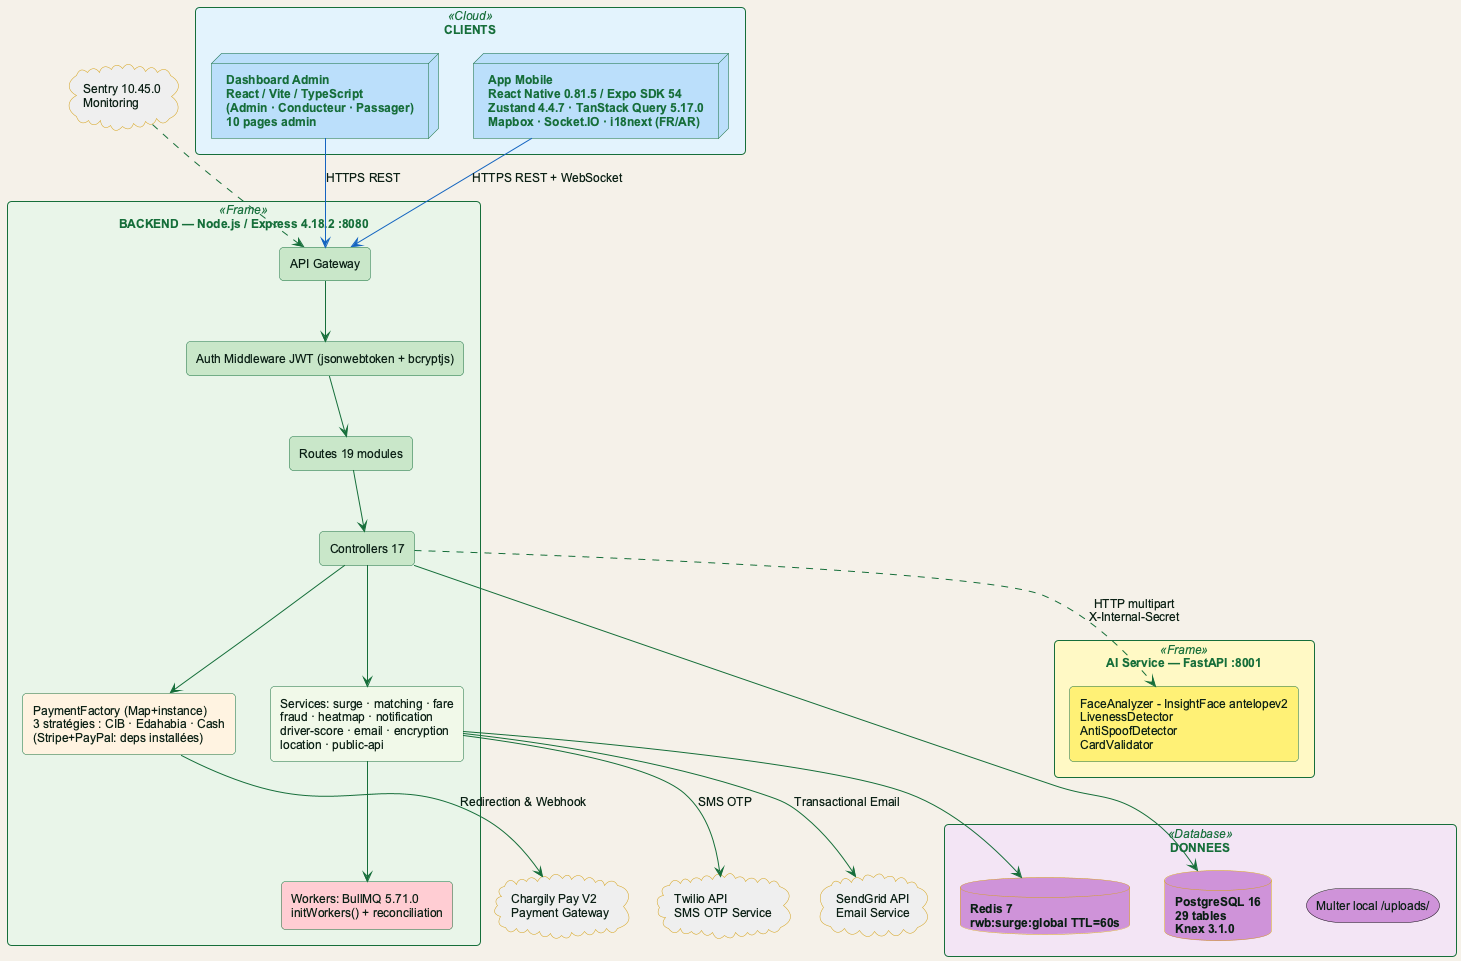
\includegraphics[width=0.95\linewidth]{fig_architecture.png}
\caption{Architecture déployée de \textit{RohWinBghit}}
\label{fig:archi-globale-r3}
\end{figure}

L'application mobile dialogue avec le \textit{back-end} principal par API \textsc{rest} et WebSocket. Le \textit{back-end} délègue les opérations de vérification d'identité au service IA via une API interne sécurisée par un secret partagé (\texttt{X-Internal-Secret}). L'ensemble est conteneurisé (Docker), exposé derrière un \textit{reverse proxy} Nginx assurant la terminaison \textsc{tls} et l'équilibrage de charge, et observé via Sentry pour les erreurs et la performance applicative.

\section{Réalisation de l'application mobile}
\label{sec:realisation-mobile}

L'application mobile expose au total \textbf{62~écrans distincts} couvrant les parcours passager et conducteur. Cette section présente les interfaces les plus représentatives, organisées par parcours fonctionnel. L'intégralité des captures est rassemblée en Annexe~D.

\subsection{Parcours \textsc{kyc} --- vérification biométrique d'identité}

La vérification \textsc{kyc} est le prérequis de toute action sensible (publication d'un trajet, réservation, paiement). Elle se déroule en trois étapes guidées~: introduction, capture de la \textsc{cin} et capture faciale avec détection de vivacité.

\begin{figure}[H]
\centering
\begin{minipage}{0.31\textwidth}
    \centering
    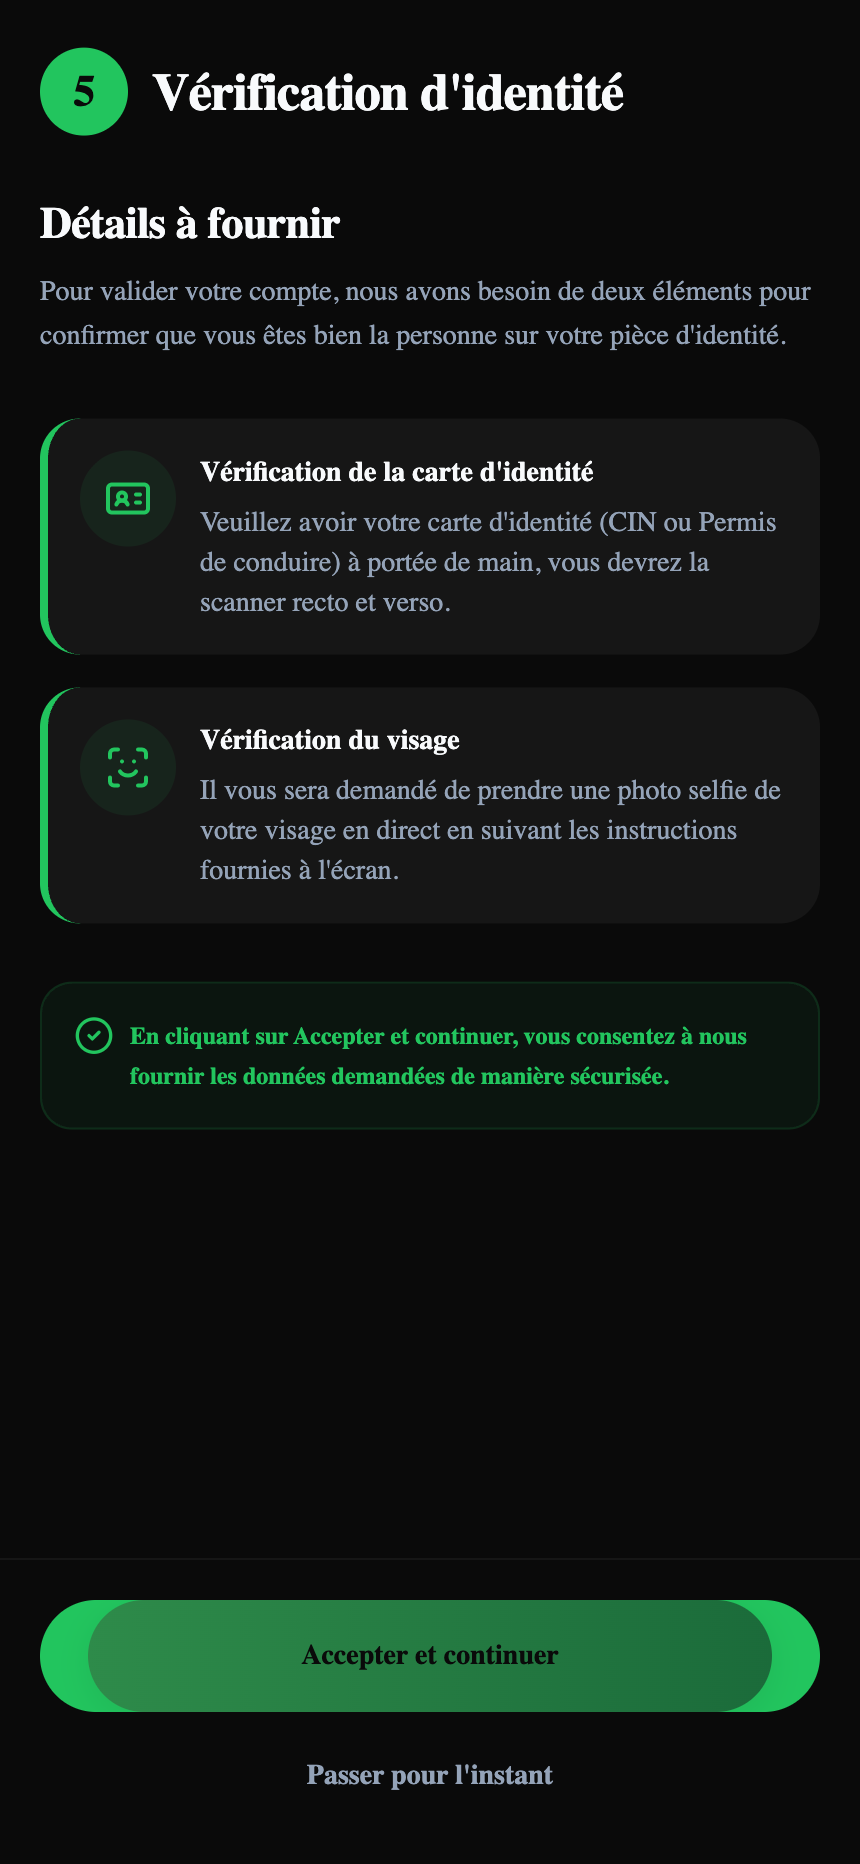
\includegraphics[width=\linewidth]{mobile-all/p_27_verif_intro.png}
    {\footnotesize \textbf{3.1a} --- Introduction \textsc{kyc}\\Documents requis, durée estimée, consentement.\par}
\end{minipage}\hfill
\begin{minipage}{0.31\textwidth}
    \centering
    
\includegraphics[width=\linewidth]{mobile-all/p_28_verif_id_capture.png}
    {\footnotesize \textbf{3.1b} --- Capture de la \textsc{cin}\\Cadre guidé recto/verso, contrôle qualité.\par}
\end{minipage}\hfill
\begin{minipage}{0.31\textwidth}
    \centering
    
\includegraphics[width=\linewidth]{mobile-all/p_29_verif_face_capture.png}
    {\footnotesize \textbf{3.1c} --- Détection de vivacité\\3 mouvements demandés, anti-\textit{spoofing} serveur.\par}
\end{minipage}
\caption{Parcours \textsc{kyc} biométrique --- étapes de capture (vue passager)}
\label{fig:kyc-screens}
\end{figure}

\begin{figure}[H]
\centering
\begin{minipage}{0.31\textwidth}
    \centering
    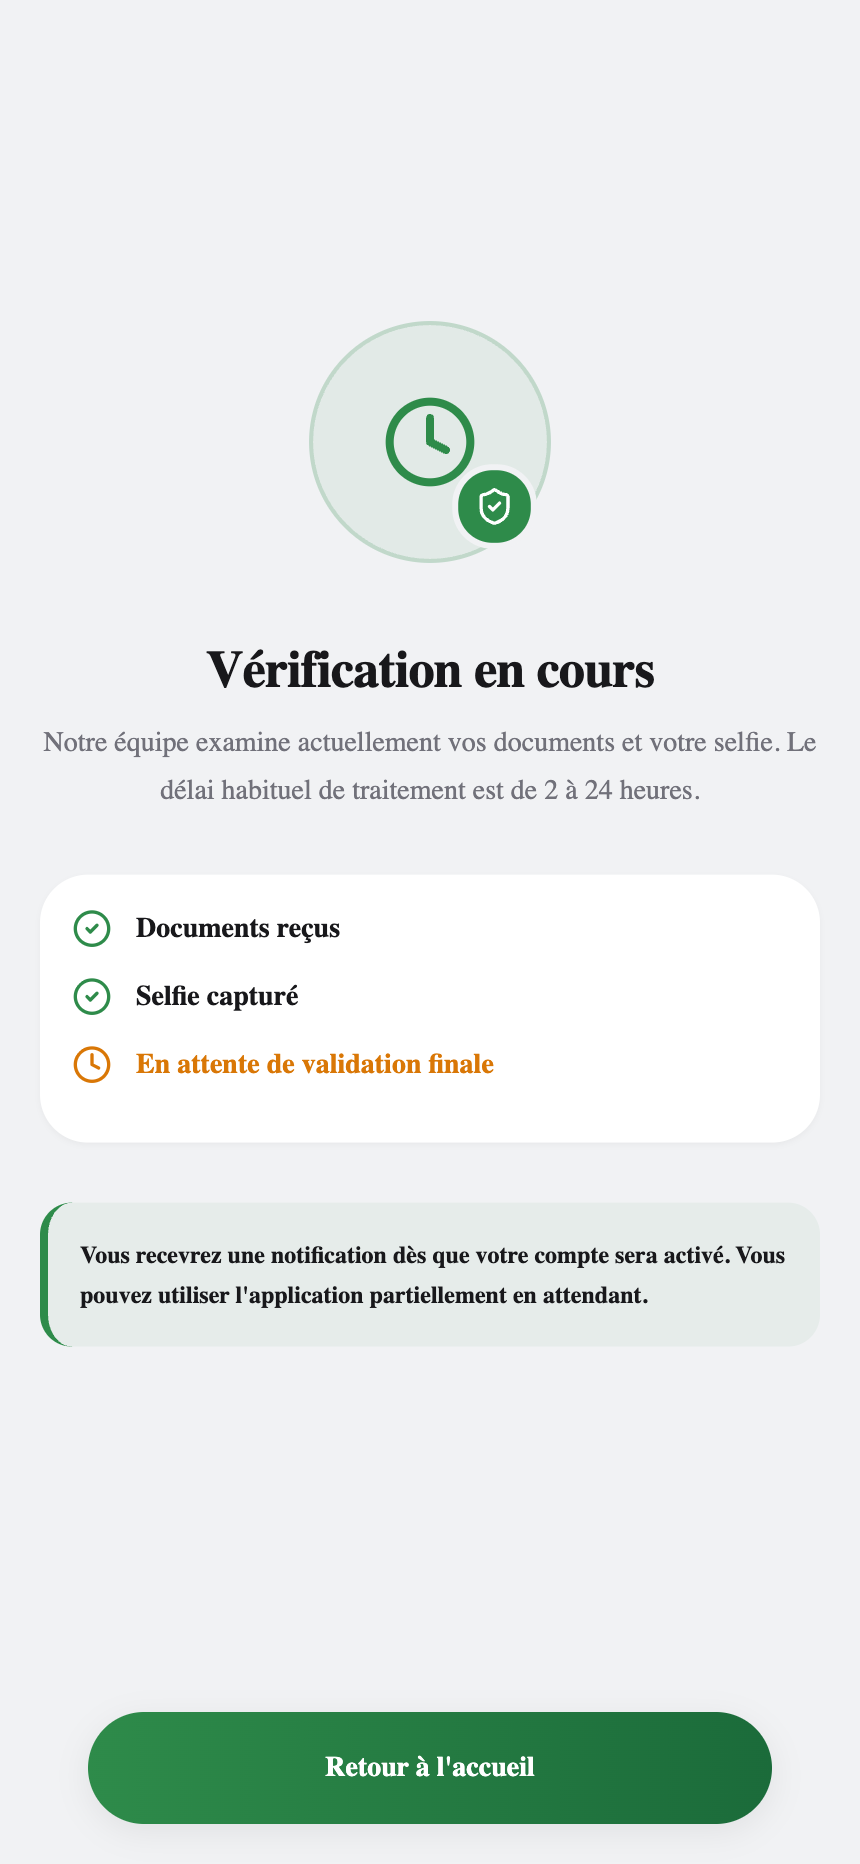
\includegraphics[width=\linewidth]{mobile-all/p_30_verif_pending.png}
    {\footnotesize \textbf{3.2a} --- Statut \textit{en attente} (passager)\\Indicateur de progression, délai estimé.\par}
\end{minipage}\hfill
\begin{minipage}{0.31\textwidth}
    \centering
    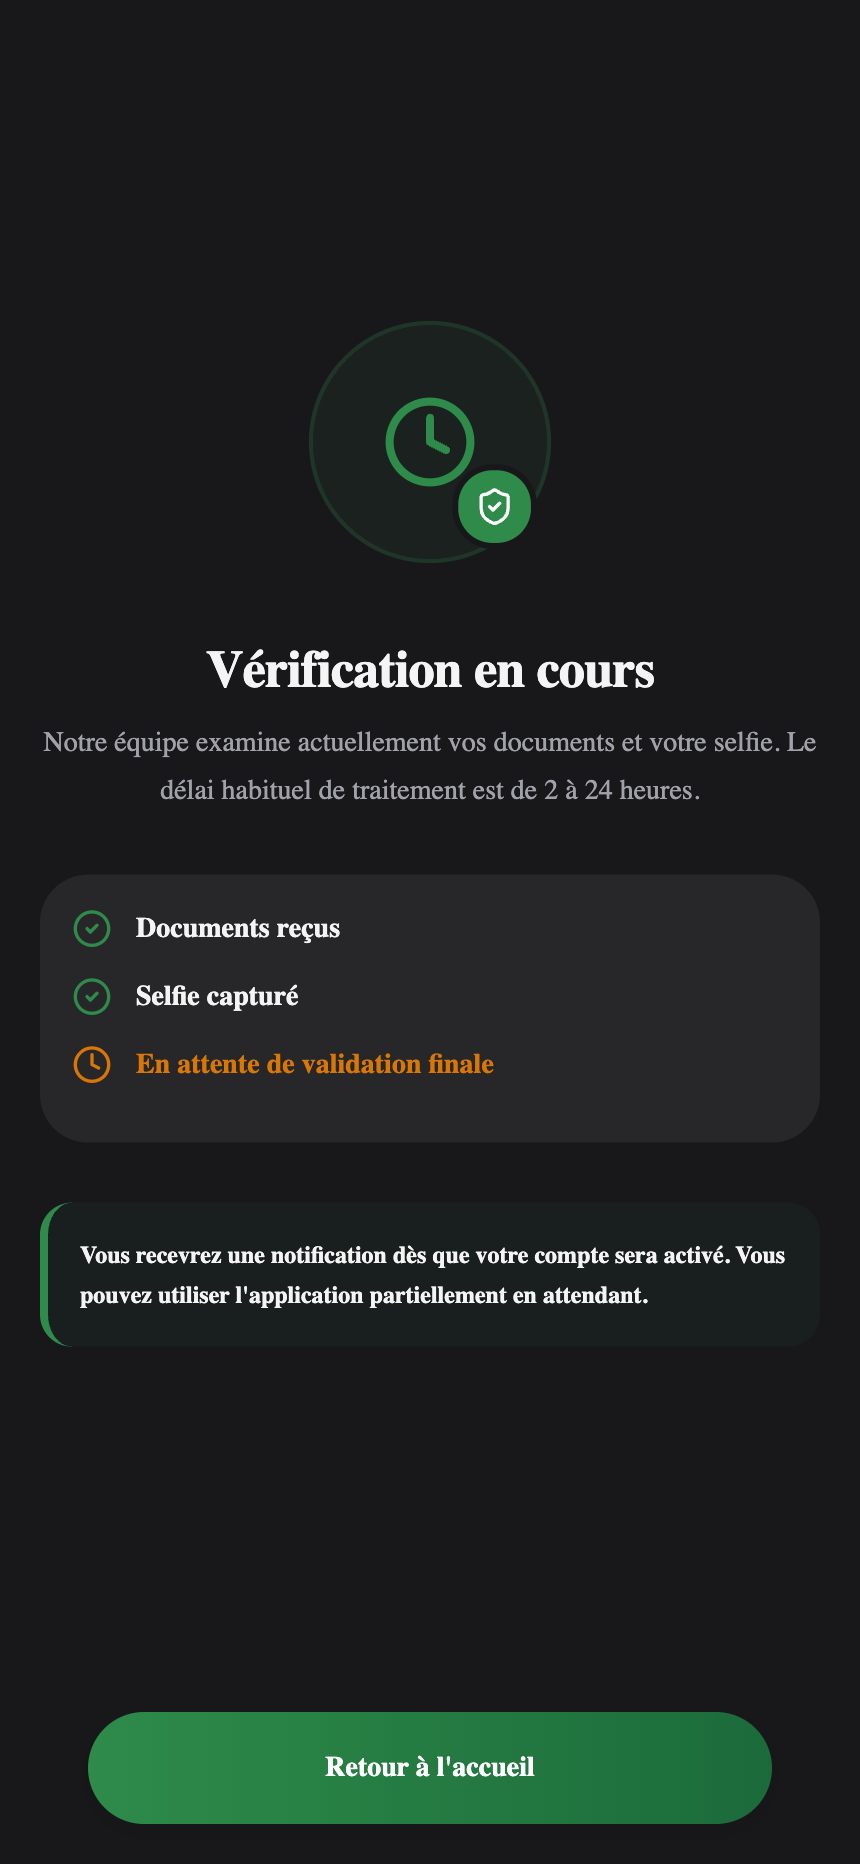
\includegraphics[width=\linewidth]{mobile-all/d_30_verif_pending.png}
    {\footnotesize \textbf{3.2b} --- Statut \textit{en attente} (conducteur)\\Même pipeline, seuils plus stricts (0,65 vs 0,60).\par}
\end{minipage}\hfill
\begin{minipage}{0.31\textwidth}
    \centering
    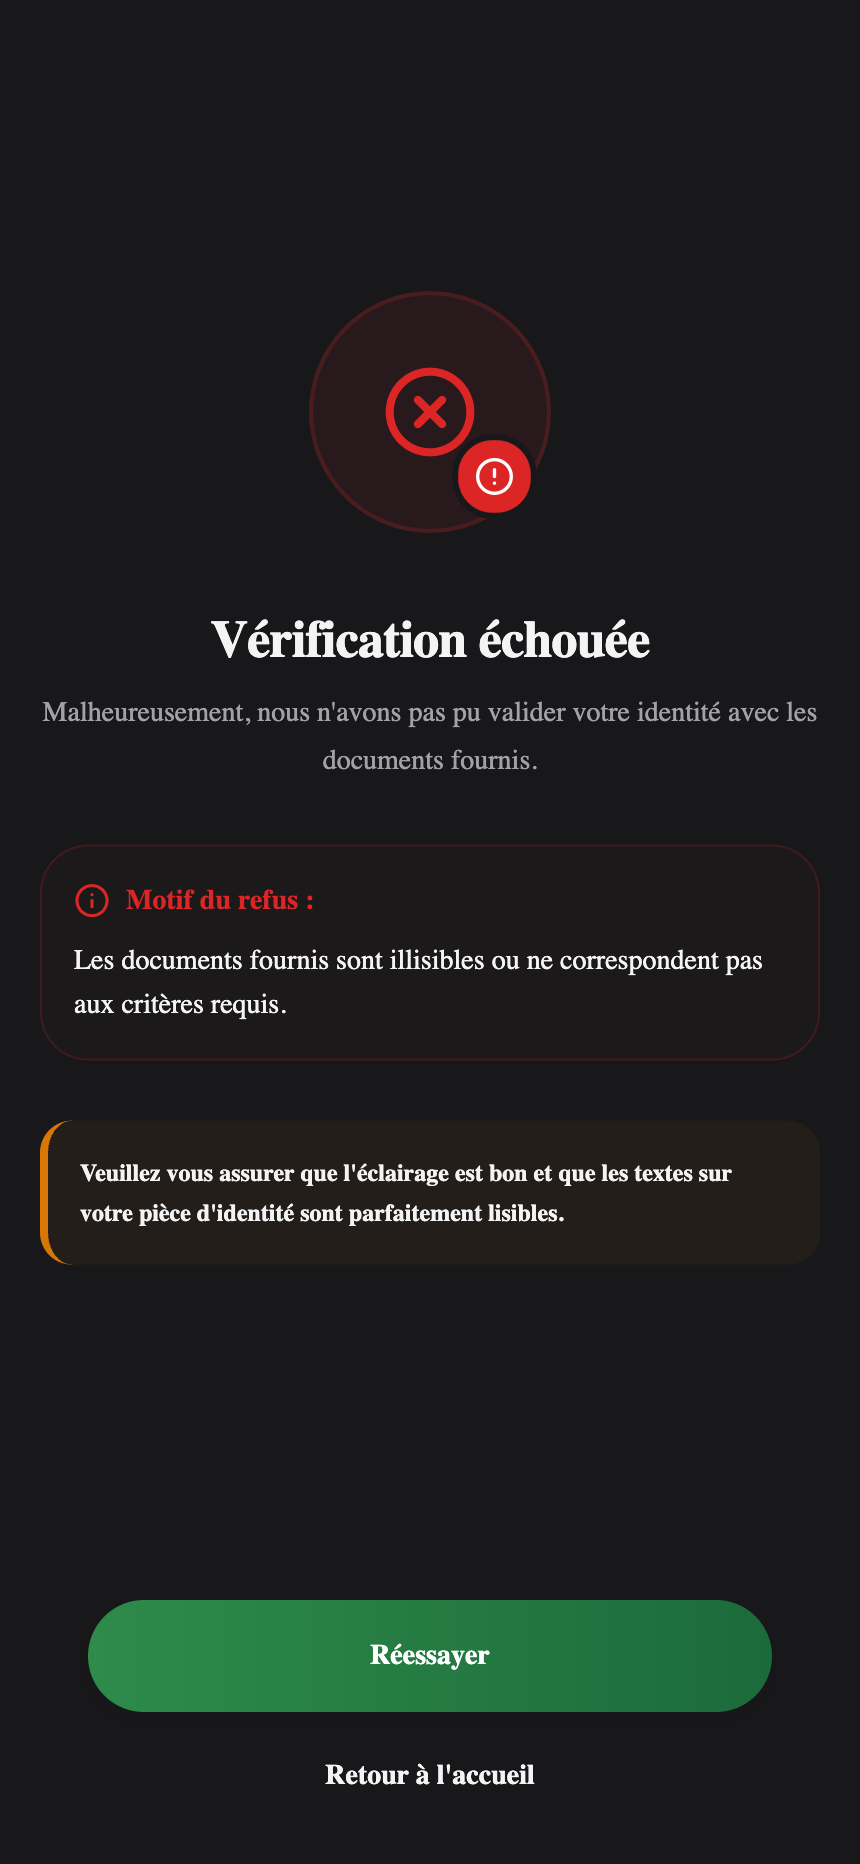
\includegraphics[width=\linewidth]{mobile-all/d_31_verif_rejected.png}
    {\footnotesize \textbf{3.2c} --- \textsc{kyc} rejeté\\Motif affiché, bouton de re-soumission activé.\par}
\end{minipage}
\caption{Parcours \textsc{kyc} biométrique --- états de vérification}
\label{fig:kyc-states}
\end{figure}

\subsection{Parcours passager --- recherche et réservation}

Le parcours passager commence par l'écran d'accueil qui agrège les suggestions personnalisées, les trajets récents et le bloc de recherche rapide.

\begin{figure}[H]
\centering
\begin{minipage}{0.31\textwidth}
    \centering
    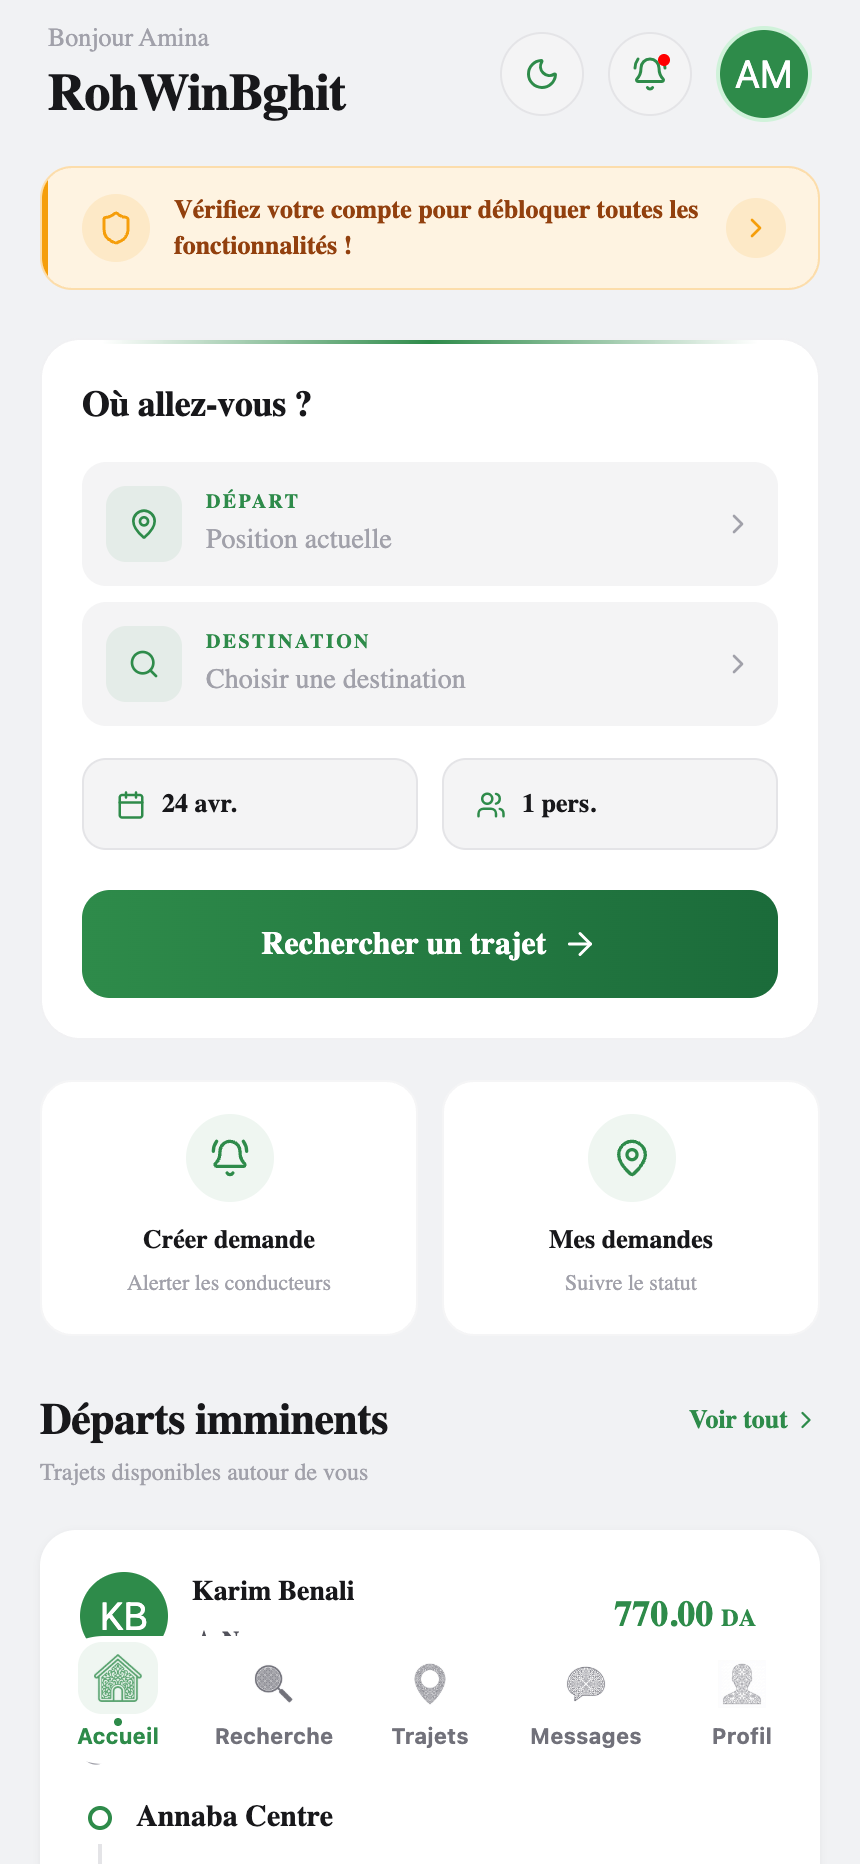
\includegraphics[width=\linewidth]{mobile-all/p_01_tab_home.png}
    {\footnotesize \textbf{3.3a} --- Tableau de bord passager\\Suggestions de trajets, raccourcis de recherche.\par}
\end{minipage}\hfill
\begin{minipage}{0.31\textwidth}
    \centering
    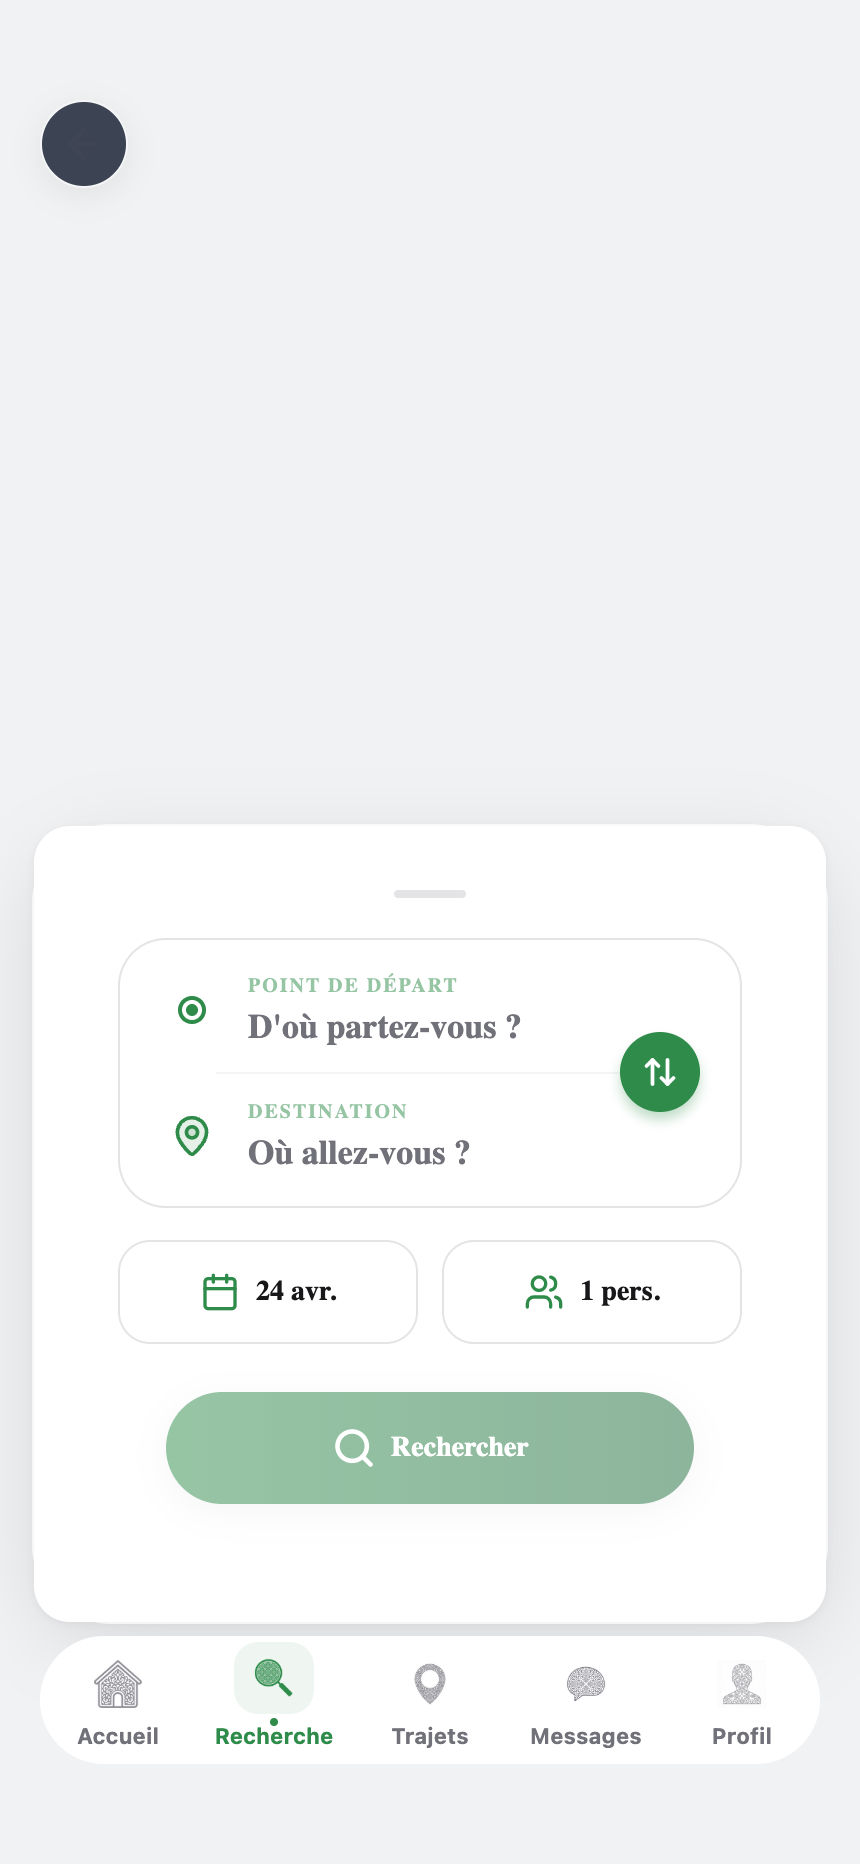
\includegraphics[width=\linewidth]{mobile-all/p_02_tab_search.png}
    {\footnotesize \textbf{3.3b} --- Recherche (formulaire)\\Wilaya départ/arrivée, date, places.\par}
\end{minipage}\hfill
\begin{minipage}{0.31\textwidth}
    \centering
    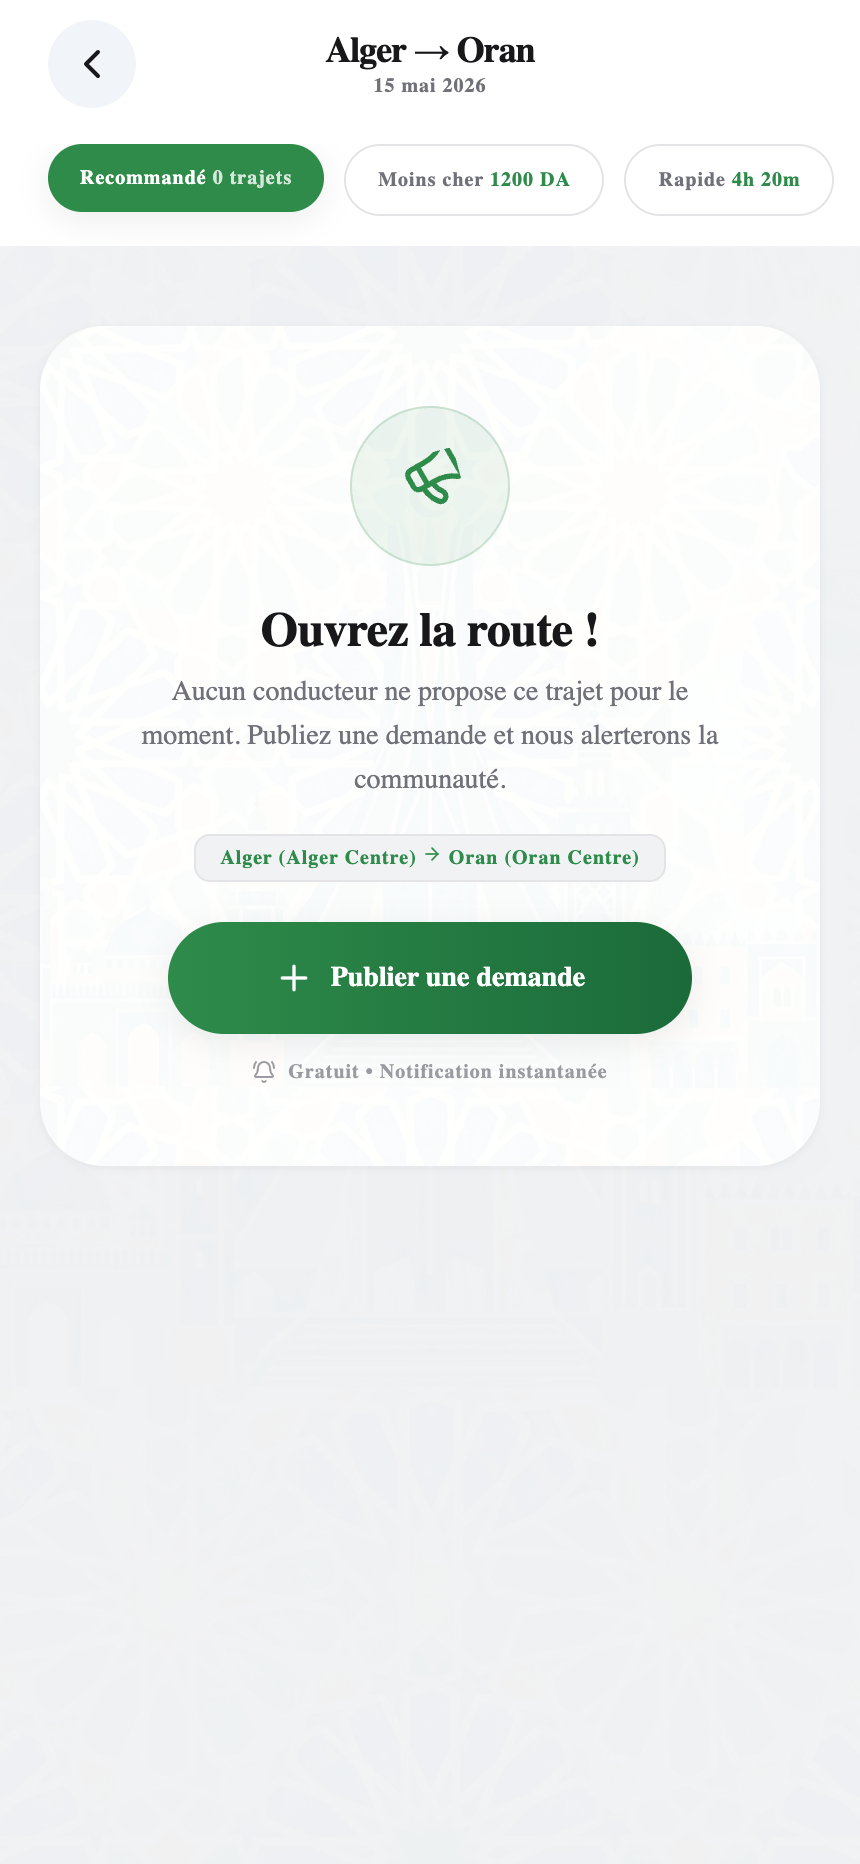
\includegraphics[width=\linewidth]{mobile-all/p_08_search_results.png}
    {\footnotesize \textbf{3.3c} --- Résultats de recherche\\Filtre prix/note/confort, tri.\par}
\end{minipage}
\caption{Parcours passager --- accueil, recherche et résultats}
\label{fig:passenger-search}
\end{figure}

\begin{figure}[H]
\centering
\begin{minipage}{0.31\textwidth}
    \centering
    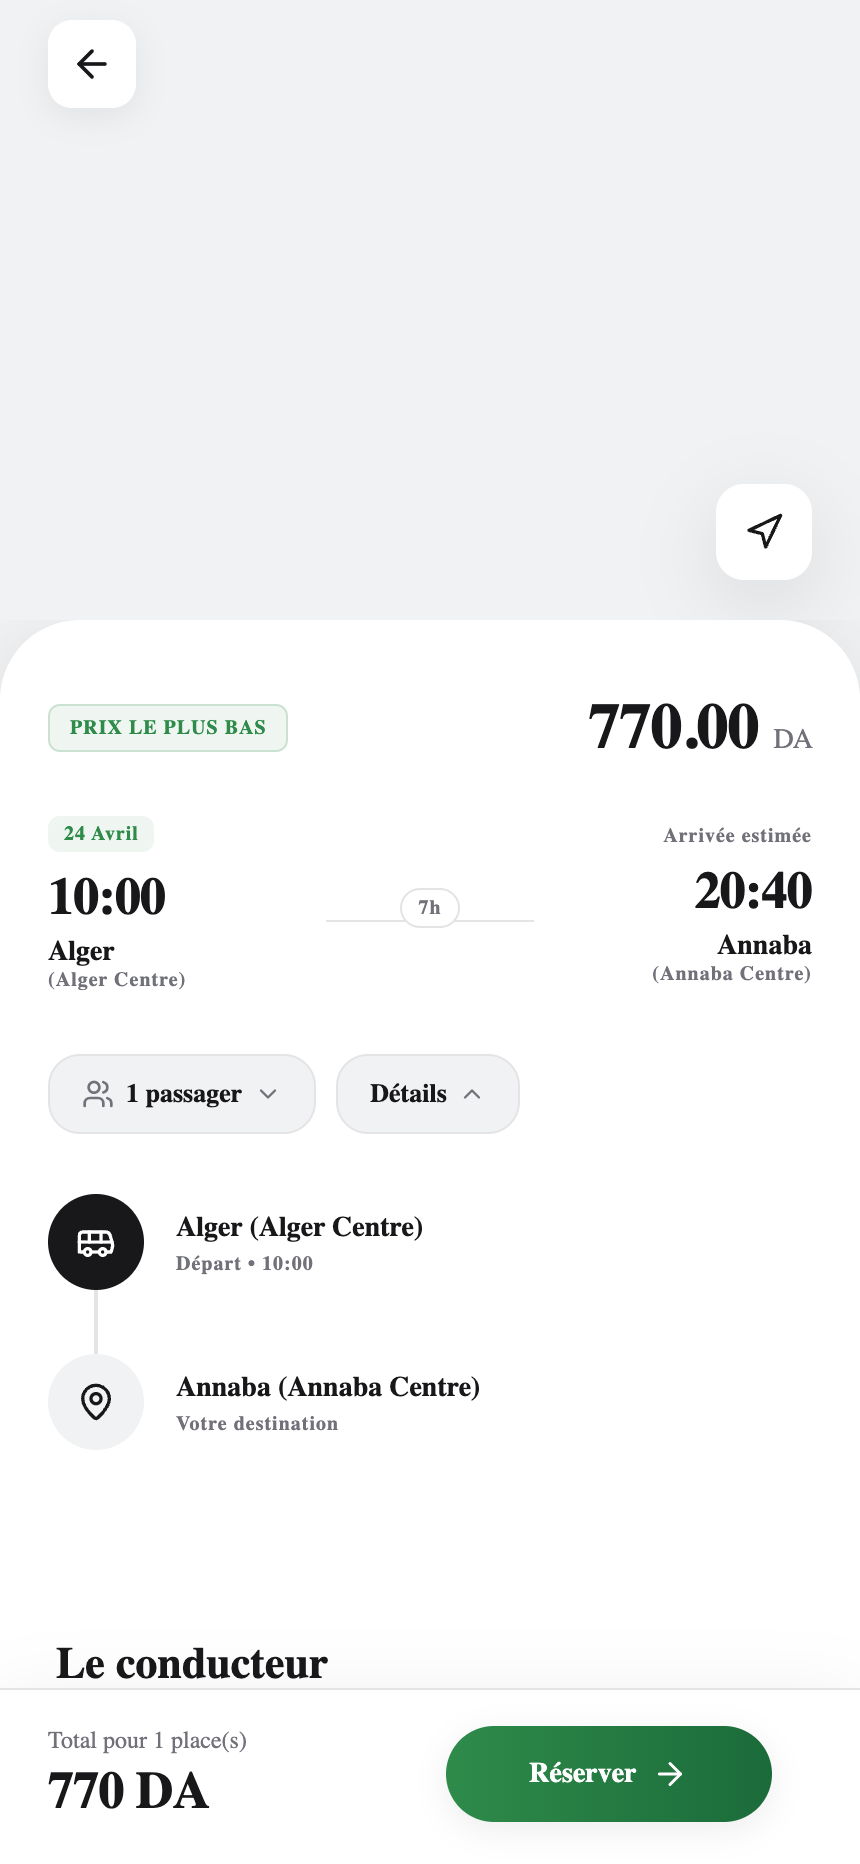
\includegraphics[width=\linewidth]{mobile-all/p_09_trip_details.png}
    {\footnotesize \textbf{3.4a} --- Détail du trajet\\Profil conducteur, itinéraire, badge \textsc{kyc}.\par}
\end{minipage}\hfill
\begin{minipage}{0.31\textwidth}
    \centering
    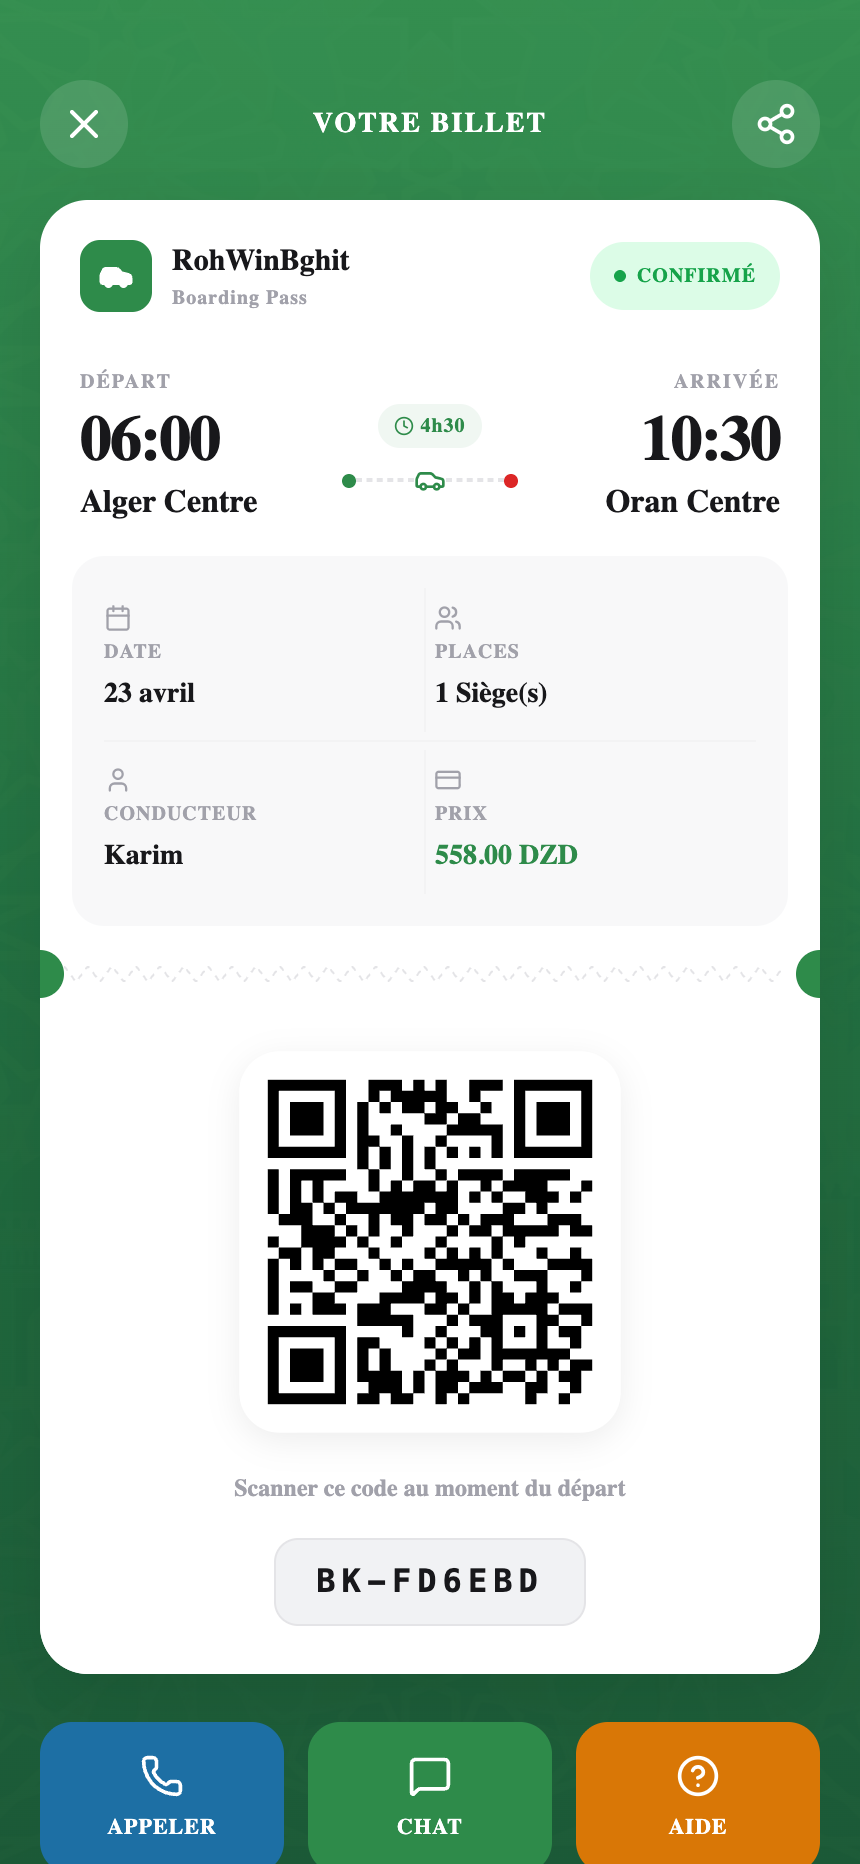
\includegraphics[width=\linewidth]{mobile-all/p_10_ticket.png}
    {\footnotesize \textbf{3.4b} --- Billet numérique\\QR code unique, récapitulatif, accès au chat.\par}
\end{minipage}\hfill
\begin{minipage}{0.31\textwidth}
    \centering
    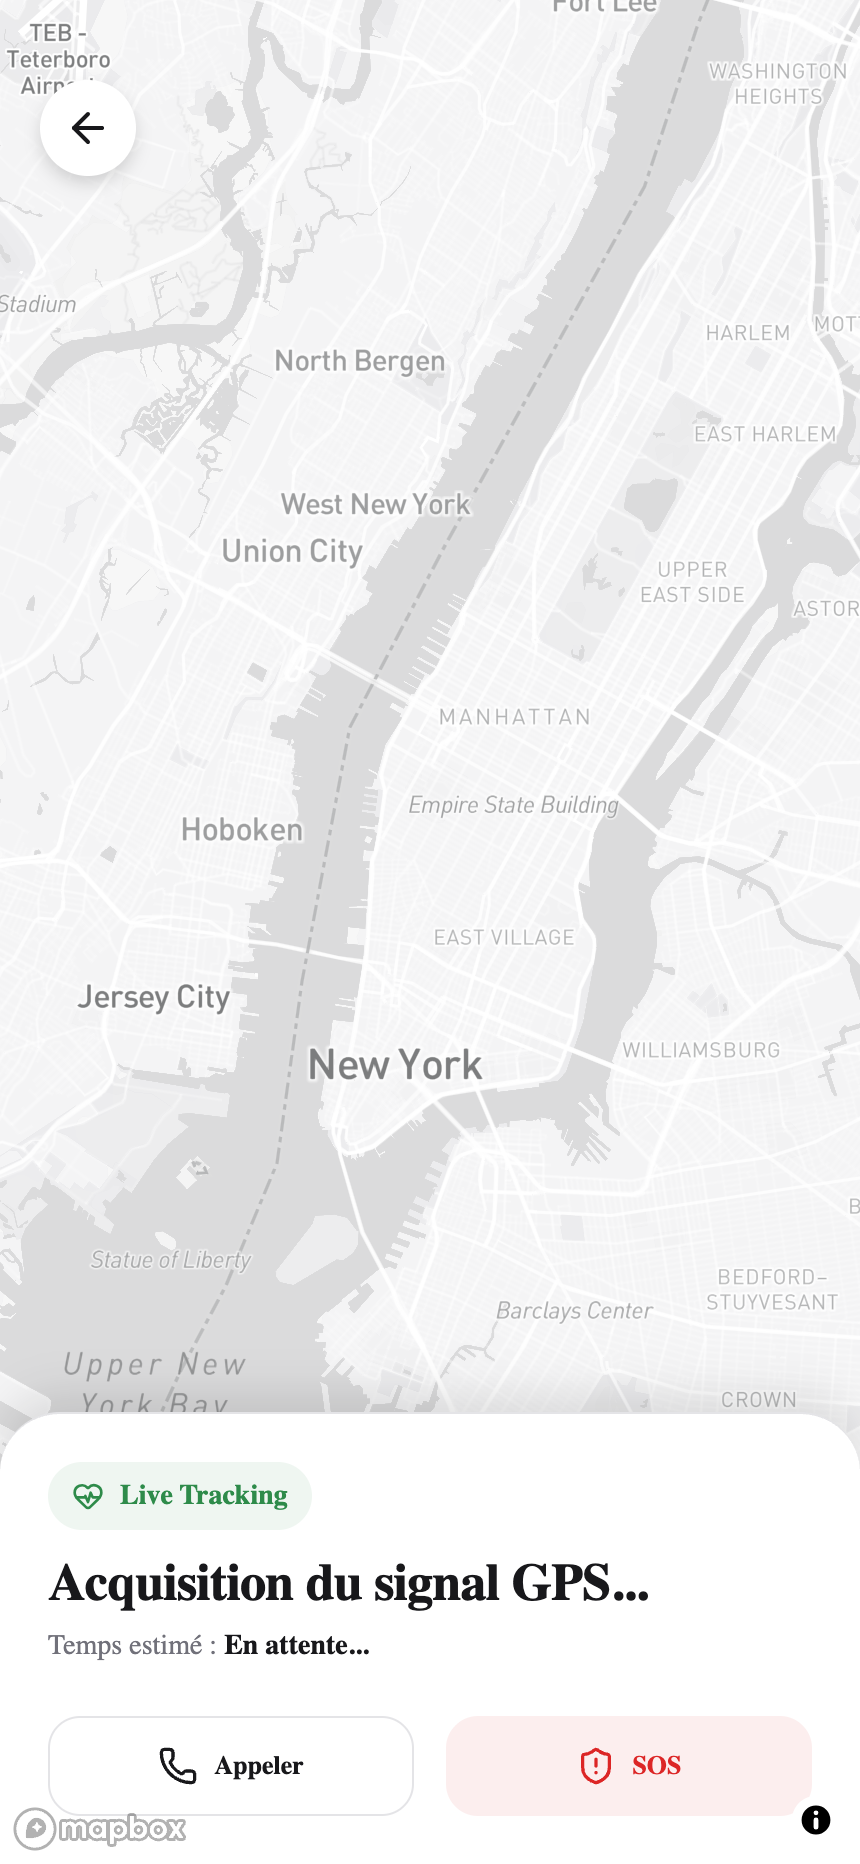
\includegraphics[width=\linewidth]{mobile-all/p_26_live_tracking.png}
    {\footnotesize \textbf{3.4c} --- Suivi GPS temps réel\\Position conducteur, ETA, bouton SOS.\par}
\end{minipage}
\caption{Parcours passager --- détail trajet, billet et suivi GPS}
\label{fig:passenger-booking}
\end{figure}

\begin{figure}[H]
\centering
\begin{minipage}{0.31\textwidth}
    \centering
    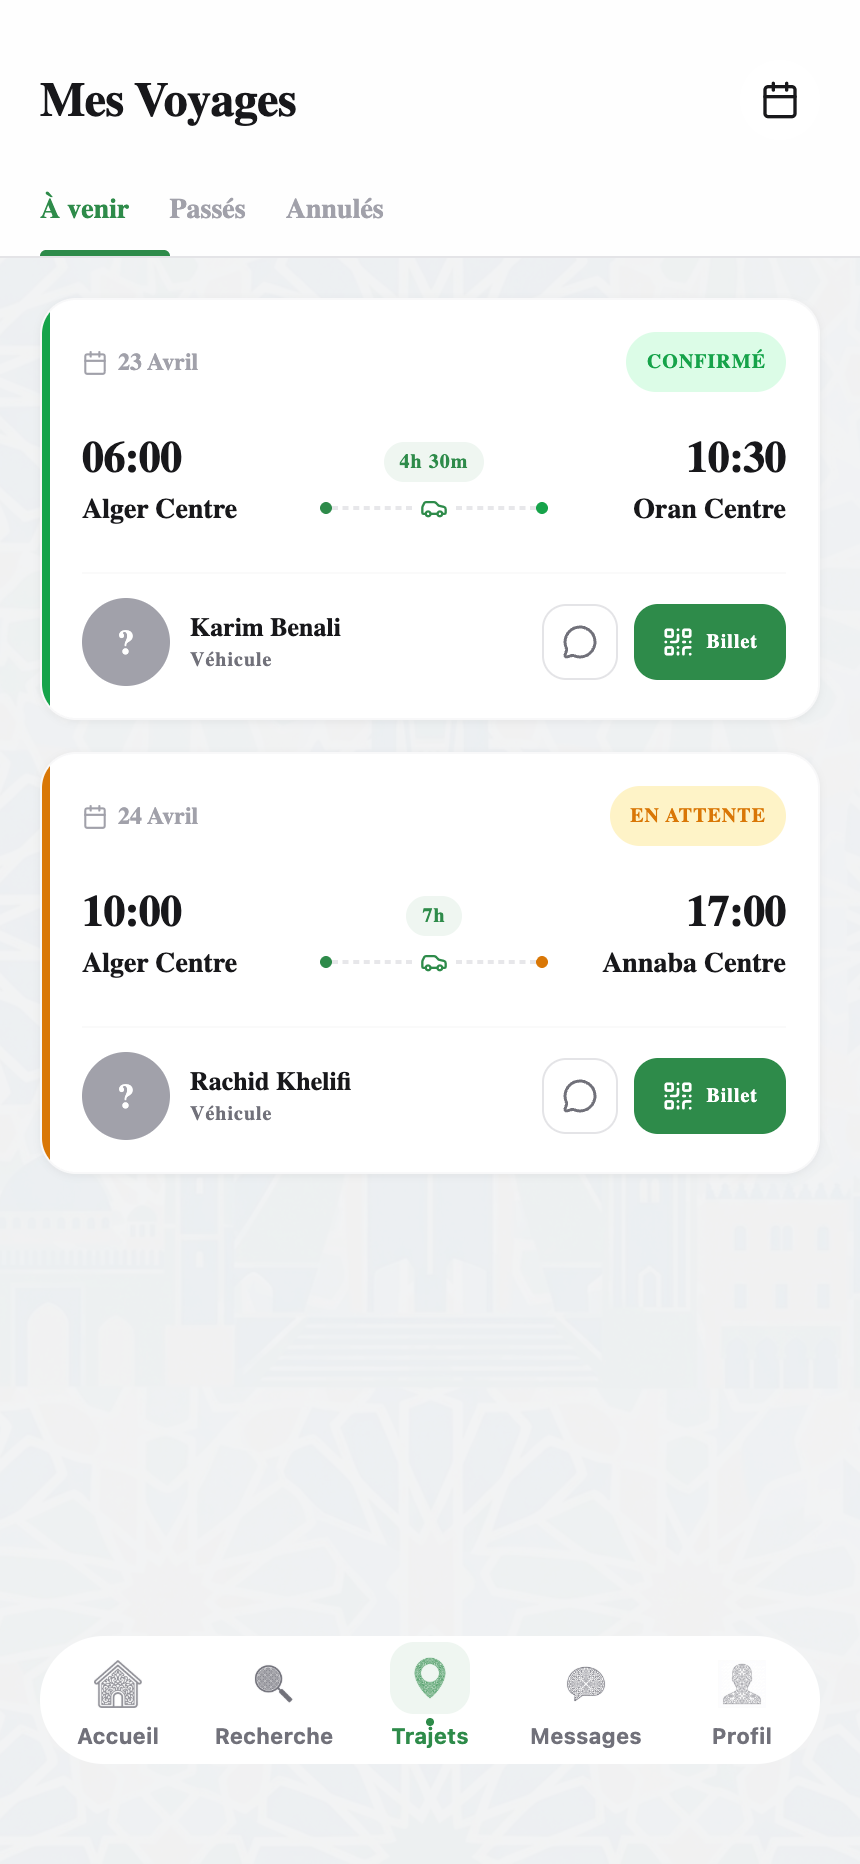
\includegraphics[width=\linewidth]{mobile-all/p_03_tab_trips.png}
    {\footnotesize \textbf{3.5a} --- Mes trajets\\Historique~: à venir / passés / annulés.\par}
\end{minipage}\hfill
\begin{minipage}{0.31\textwidth}
    \centering
    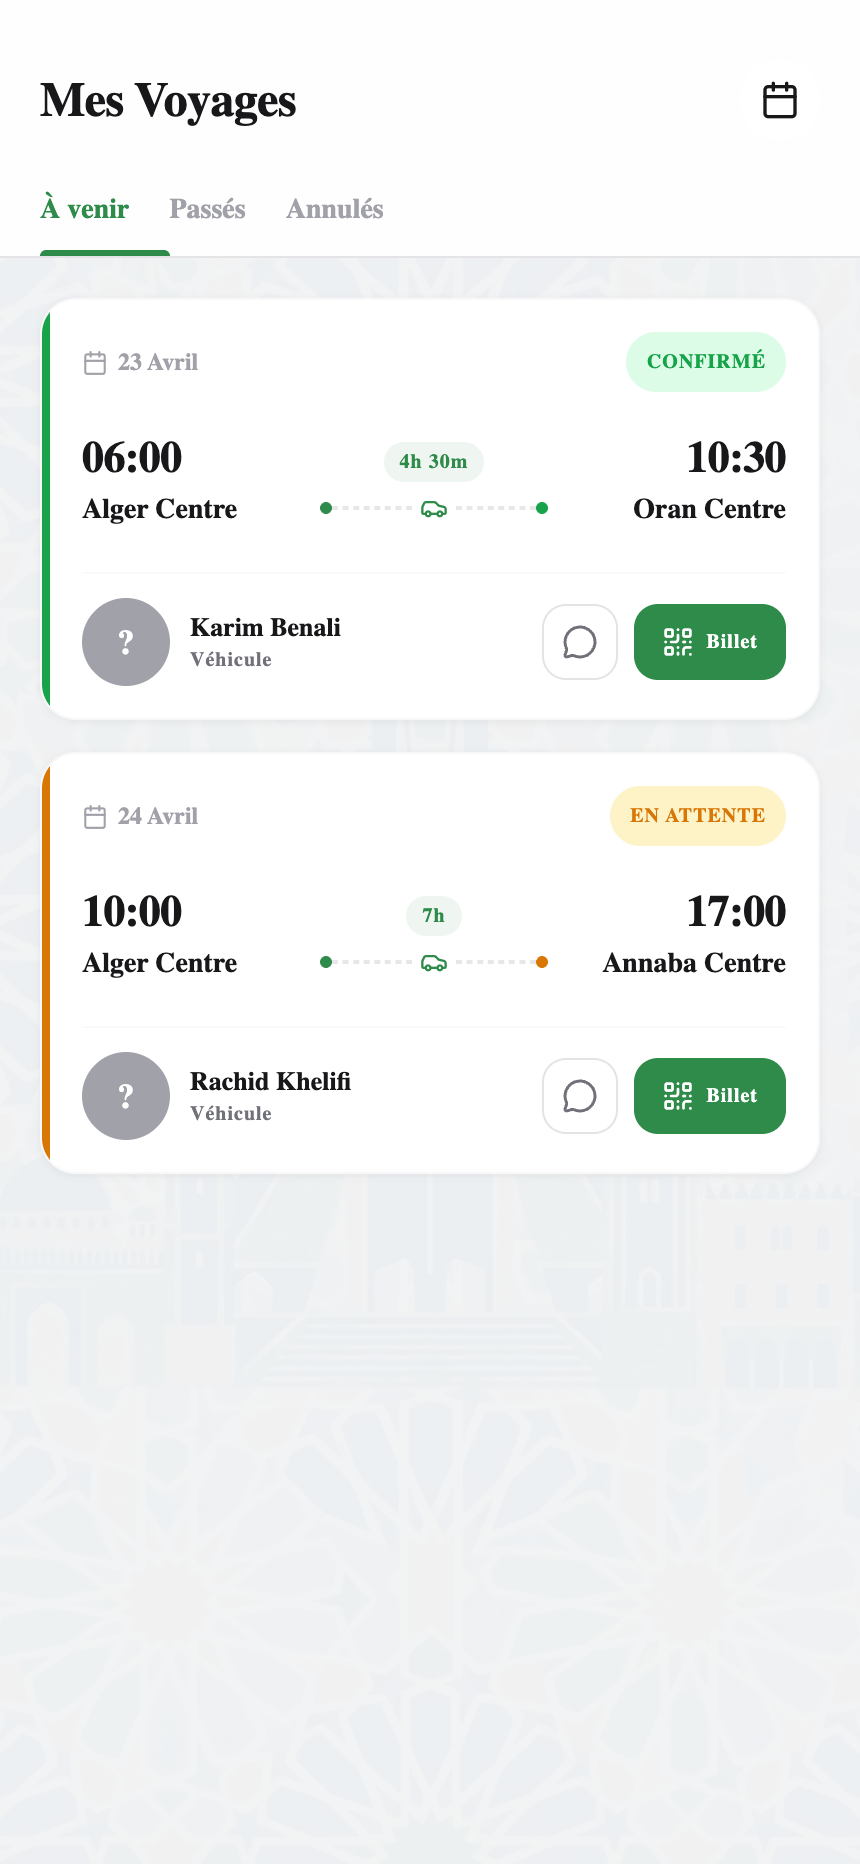
\includegraphics[width=\linewidth]{mobile-all/p_06_trips_upcoming.png}
    {\footnotesize \textbf{3.5b} --- Trajets à venir\\Détails de la réservation, bouton annulation.\par}
\end{minipage}\hfill
\begin{minipage}{0.31\textwidth}
    \centering
    
\includegraphics[width=\linewidth]{mobile-all/p_07_trips_past.png}
    {\footnotesize \textbf{3.5c} --- Trajets passés\\Accès à la notation post-trajet.\par}
\end{minipage}
\caption{Parcours passager --- gestion des trajets}
\label{fig:passenger-trips}
\end{figure}

\begin{figure}[H]
\centering
\begin{minipage}{0.31\textwidth}
    \centering
    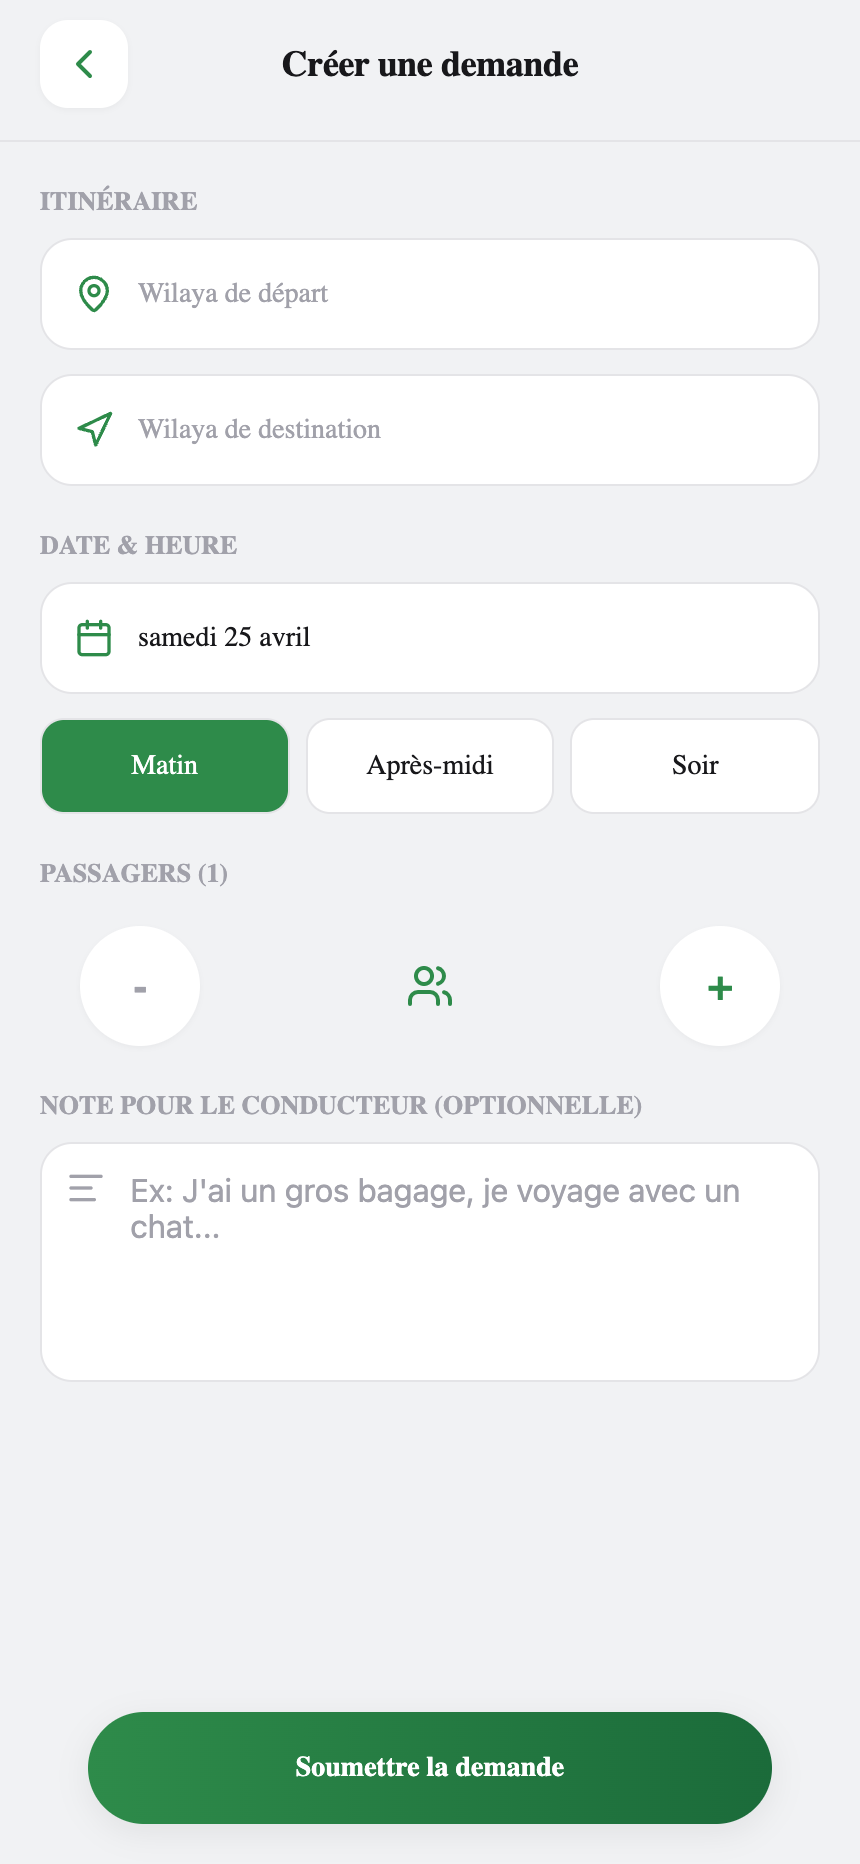
\includegraphics[width=\linewidth]{mobile-all/p_11_create_trip_request.png}
    {\footnotesize \textbf{3.6a} --- Créer une demande de trajet\\\textit{Matching} inverse~: le passager publie son besoin.\par}
\end{minipage}\hfill
\begin{minipage}{0.31\textwidth}
    \centering
    
\includegraphics[width=\linewidth]{mobile-all/p_12_my_trip_requests.png}
    {\footnotesize \textbf{3.6b} --- Mes demandes de trajet\\Suivi en attente / matchées / expirées.\par}
\end{minipage}\hfill
\begin{minipage}{0.31\textwidth}
    \centering
    
\includegraphics[width=\linewidth]{mobile-all/p_04_tab_messages.png}
    {\footnotesize \textbf{3.6c} --- Messagerie\\Chat Socket.IO, sans échange de numéro.\par}
\end{minipage}
\caption{Parcours passager --- demandes de trajet et messagerie}
\label{fig:passenger-requests}
\end{figure}

\begin{figure}[H]
\centering
\begin{minipage}{0.31\textwidth}
    \centering
    
\includegraphics[width=\linewidth]{mobile-all/p_15_payment_methods.png}
    {\footnotesize \textbf{3.7a} --- Méthodes de paiement\\\textsc{cib}, \textit{Edahabia} (\textit{sandbox}), espèces.\par}
\end{minipage}\hfill
\begin{minipage}{0.31\textwidth}
    \centering
    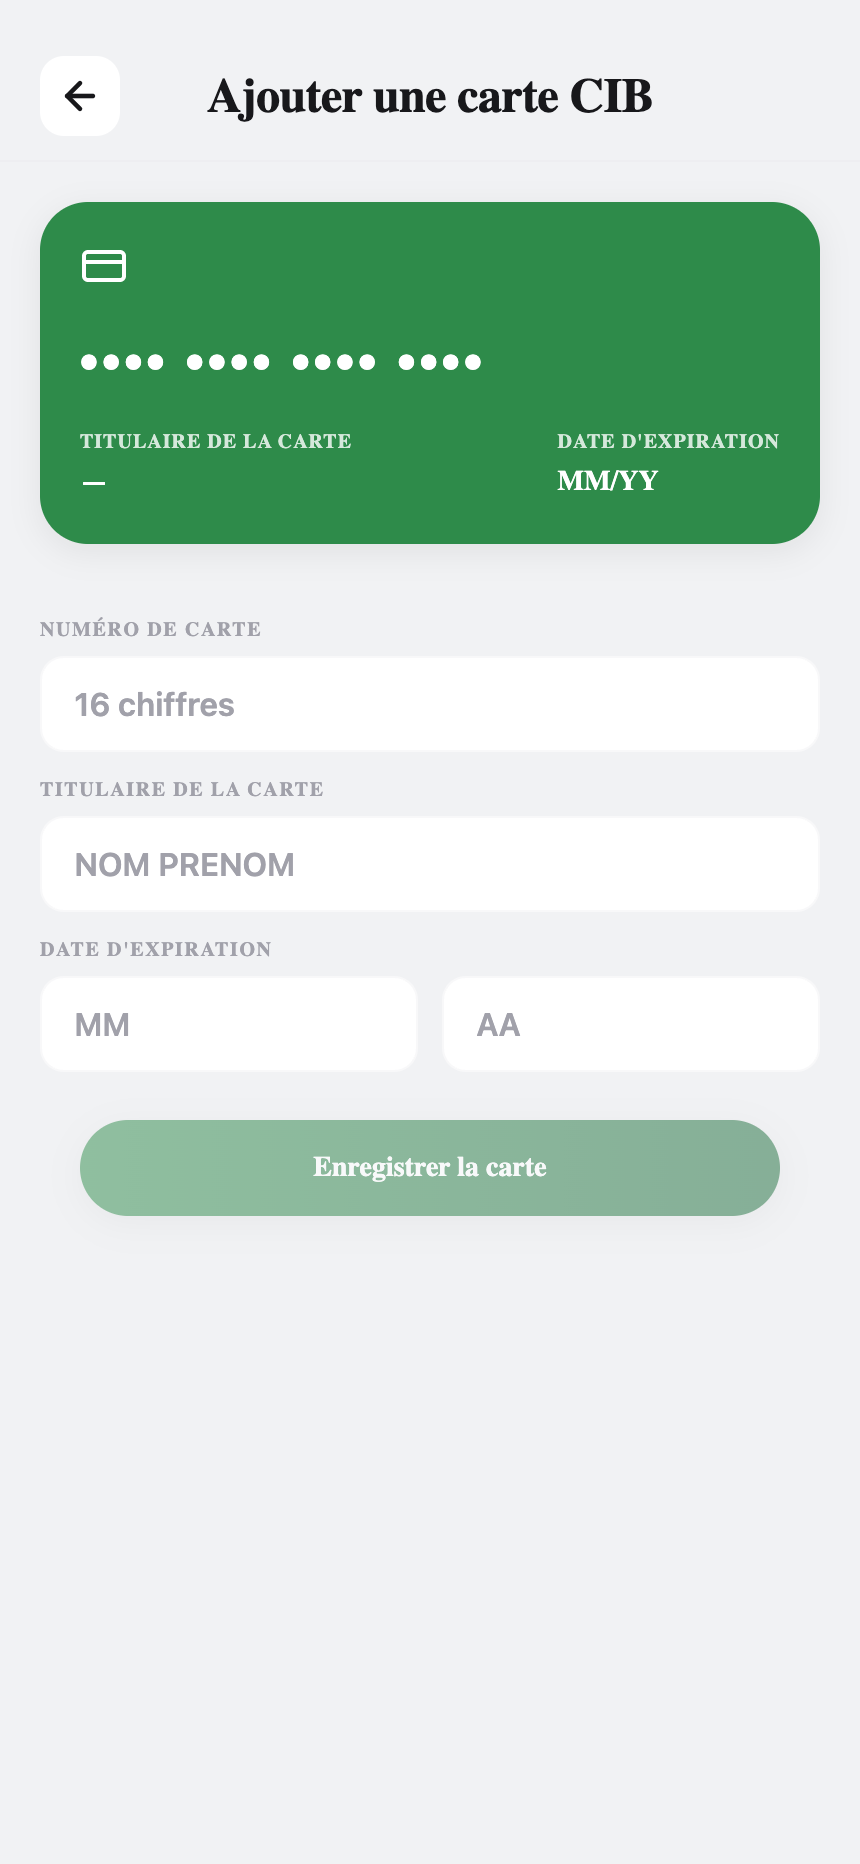
\includegraphics[width=\linewidth]{mobile-all/p_16_add_card.png}
    {\footnotesize \textbf{3.7b} --- Ajout d'une carte\\Formulaire \textsc{cib}/\textit{Edahabia}, validation \textsc{satim}.\par}
\end{minipage}\hfill
\begin{minipage}{0.31\textwidth}
    \centering
    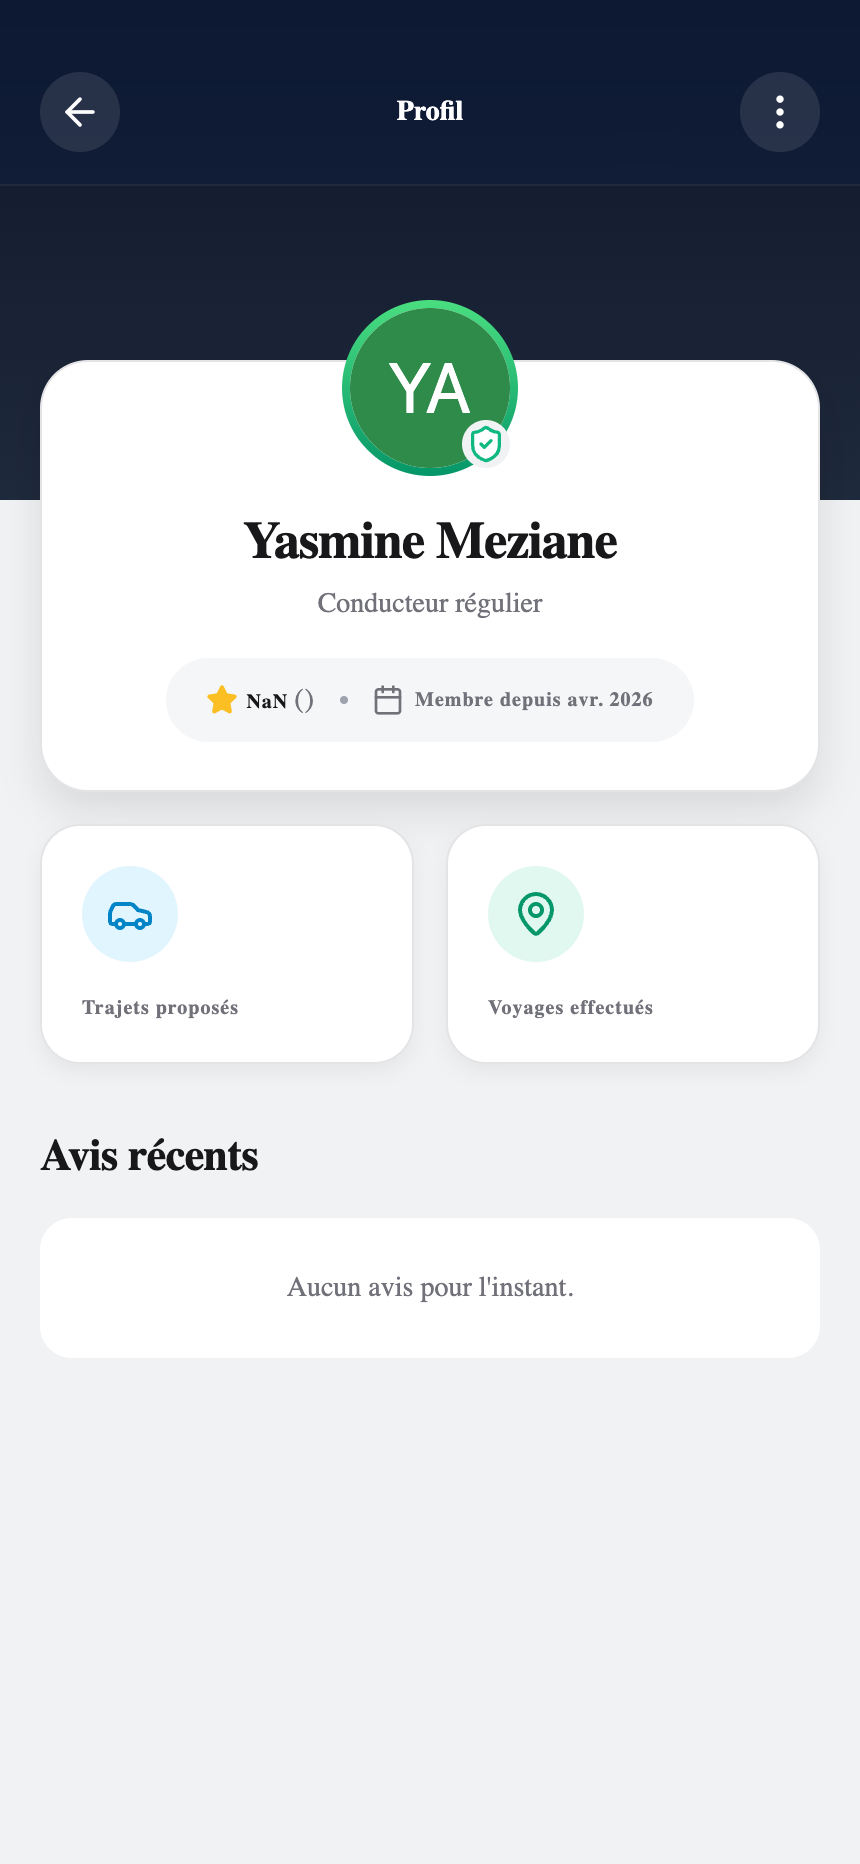
\includegraphics[width=\linewidth]{mobile-all/p_13_public_profile.png}
    {\footnotesize \textbf{3.7c} --- Profil public passager\\Note, historique, badge \textsc{kyc} vérifié.\par}
\end{minipage}
\caption{Parcours passager --- paiement et profil public}
\label{fig:passenger-misc}
\end{figure}

\subsection{Parcours conducteur --- publication et gestion}

Le conducteur accède à un tableau de bord dédié affichant ses gains mensuels, le nombre de trajets effectués, sa note moyenne et ses demandes de réservation en attente.

\begin{figure}[H]
\centering
\begin{minipage}{0.31\textwidth}
    \centering
    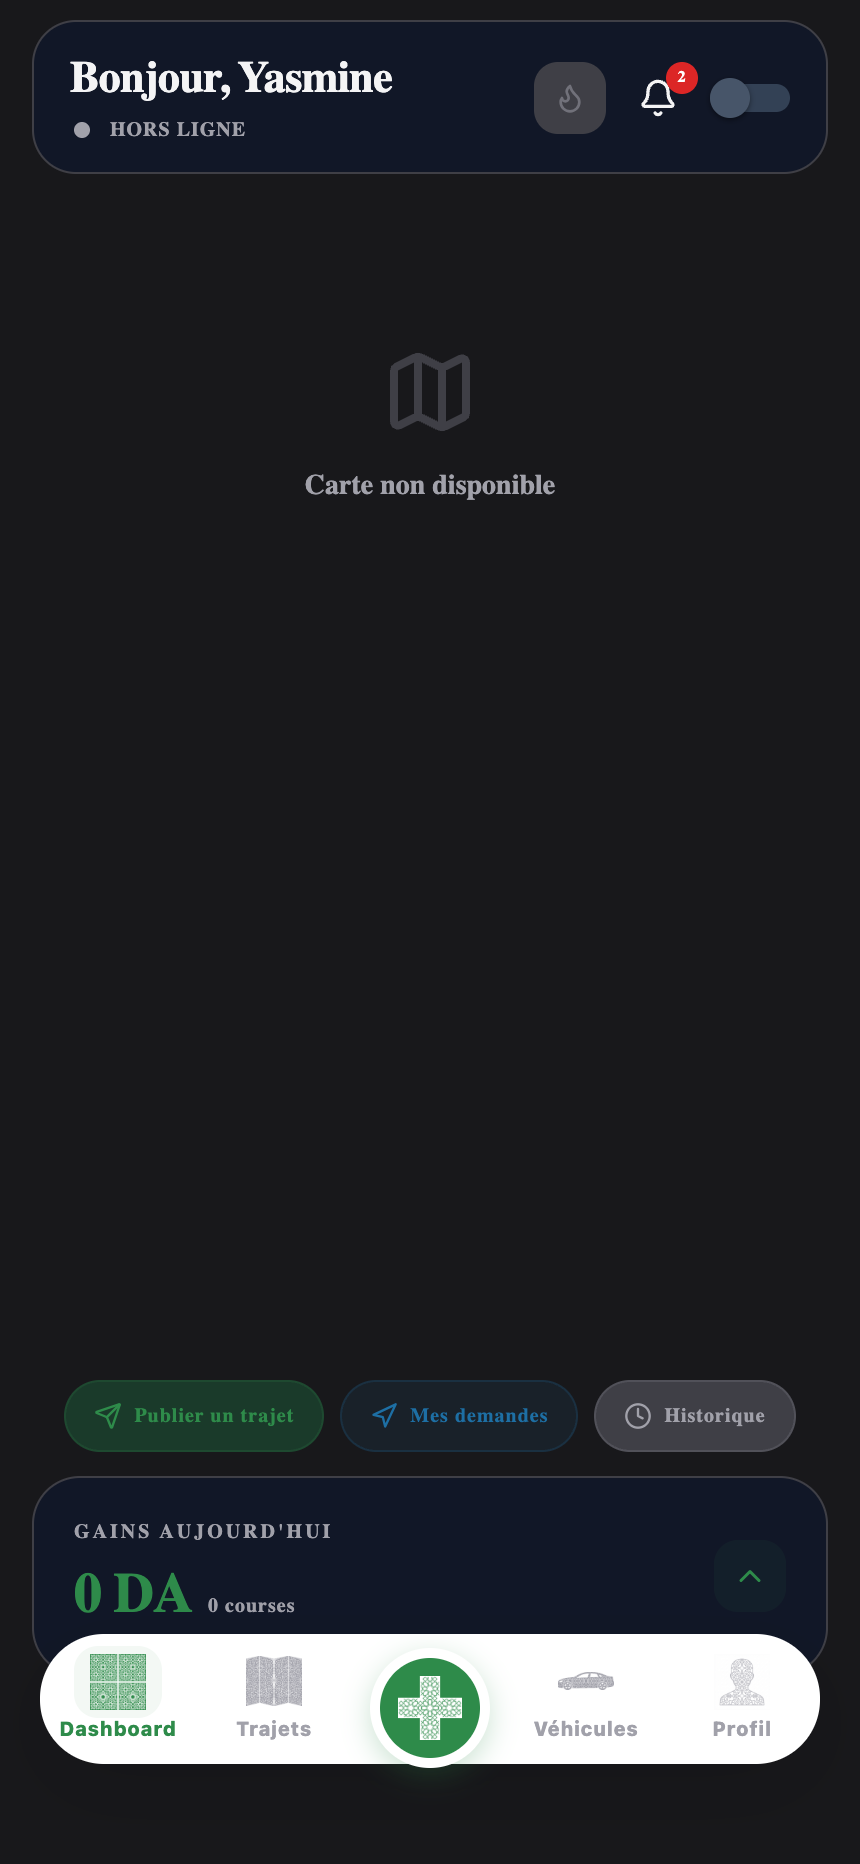
\includegraphics[width=\linewidth]{mobile-all/d_01_tab_dashboard.png}
    {\footnotesize \textbf{3.8a} --- Tableau de bord conducteur\\KPIs personnels, alertes \textsc{kyc}.\par}
\end{minipage}\hfill
\begin{minipage}{0.31\textwidth}
    \centering
    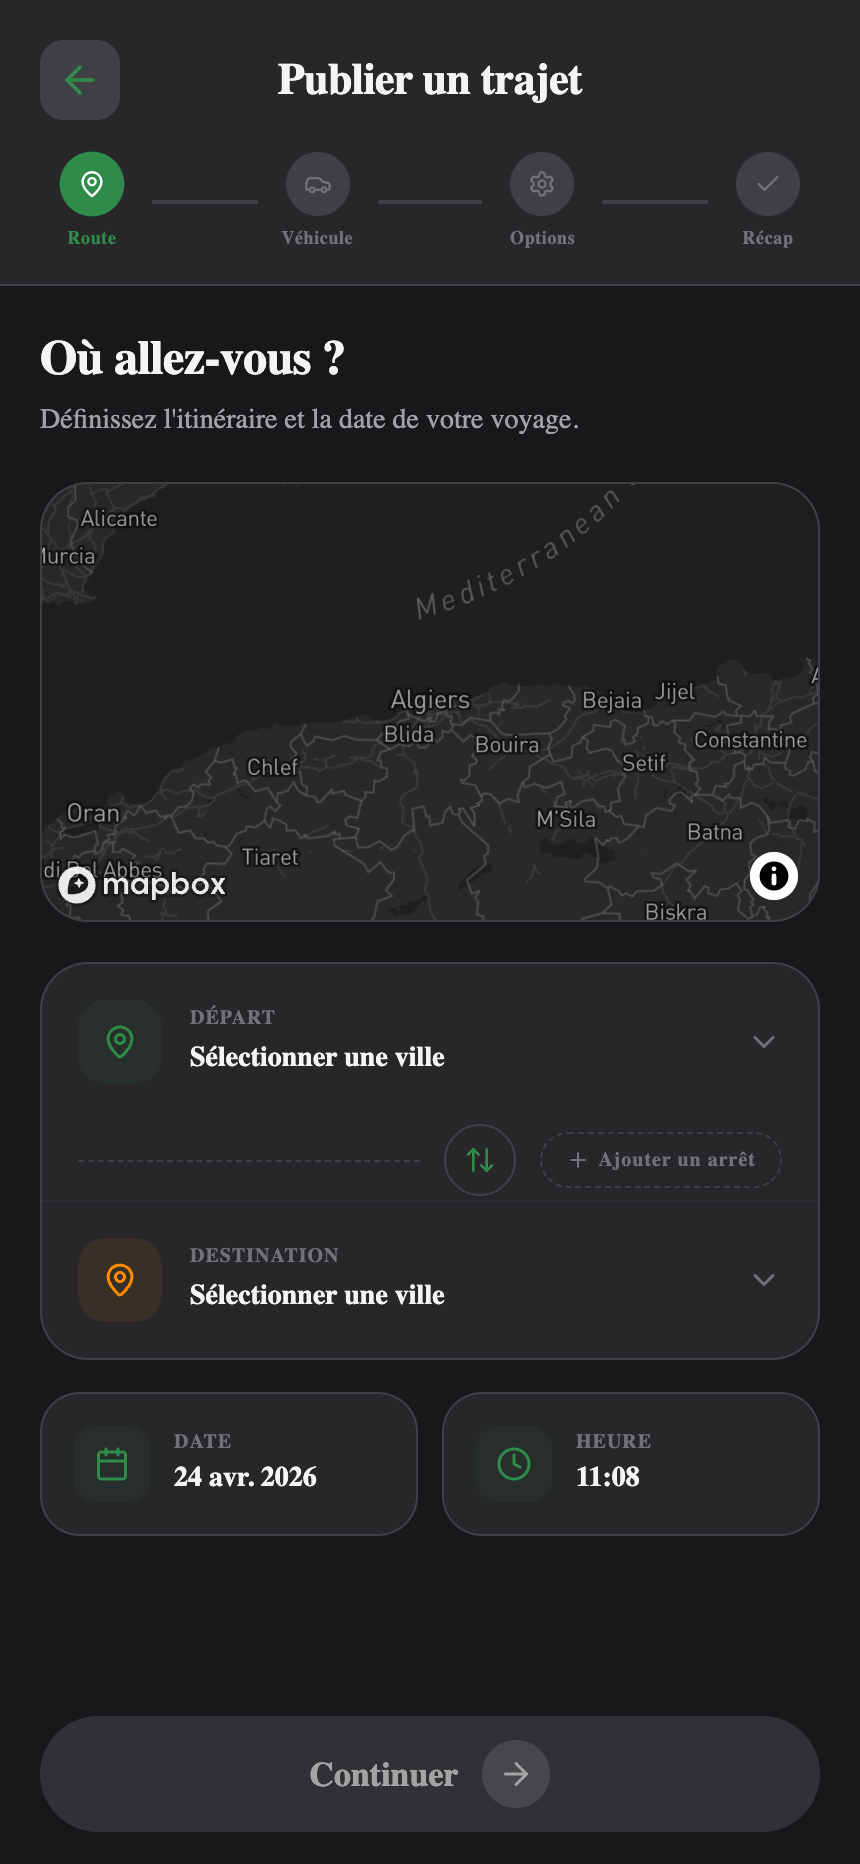
\includegraphics[width=\linewidth]{mobile-all/d_03_tab_publish.png}
    {\footnotesize \textbf{3.8b} --- Publication d'un trajet\\Formulaire complet, prix suggéré.\par}
\end{minipage}\hfill
\begin{minipage}{0.31\textwidth}
    \centering
    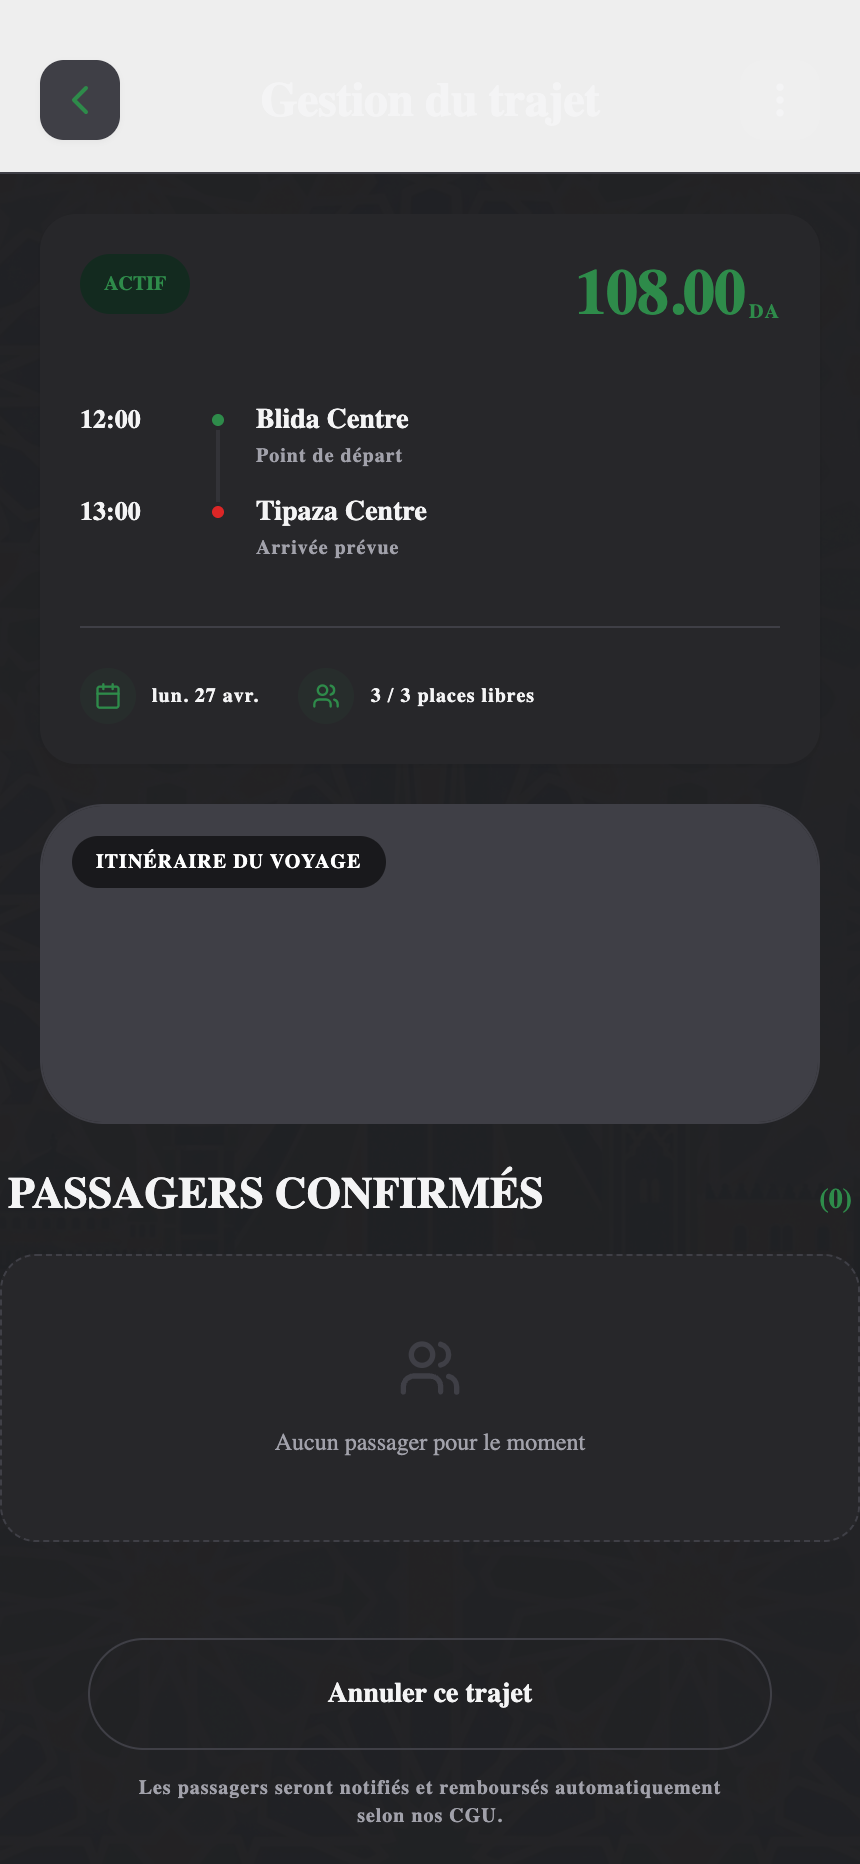
\includegraphics[width=\linewidth]{mobile-all/d_06_trip_manage.png}
    {\footnotesize \textbf{3.8c} --- Gestion du trajet\\Liste des passagers, démarrer/terminer.\par}
\end{minipage}
\caption{Parcours conducteur --- tableau de bord, publication et gestion}
\label{fig:driver-main}
\end{figure}

\begin{figure}[H]
\centering
\begin{minipage}{0.31\textwidth}
    \centering
    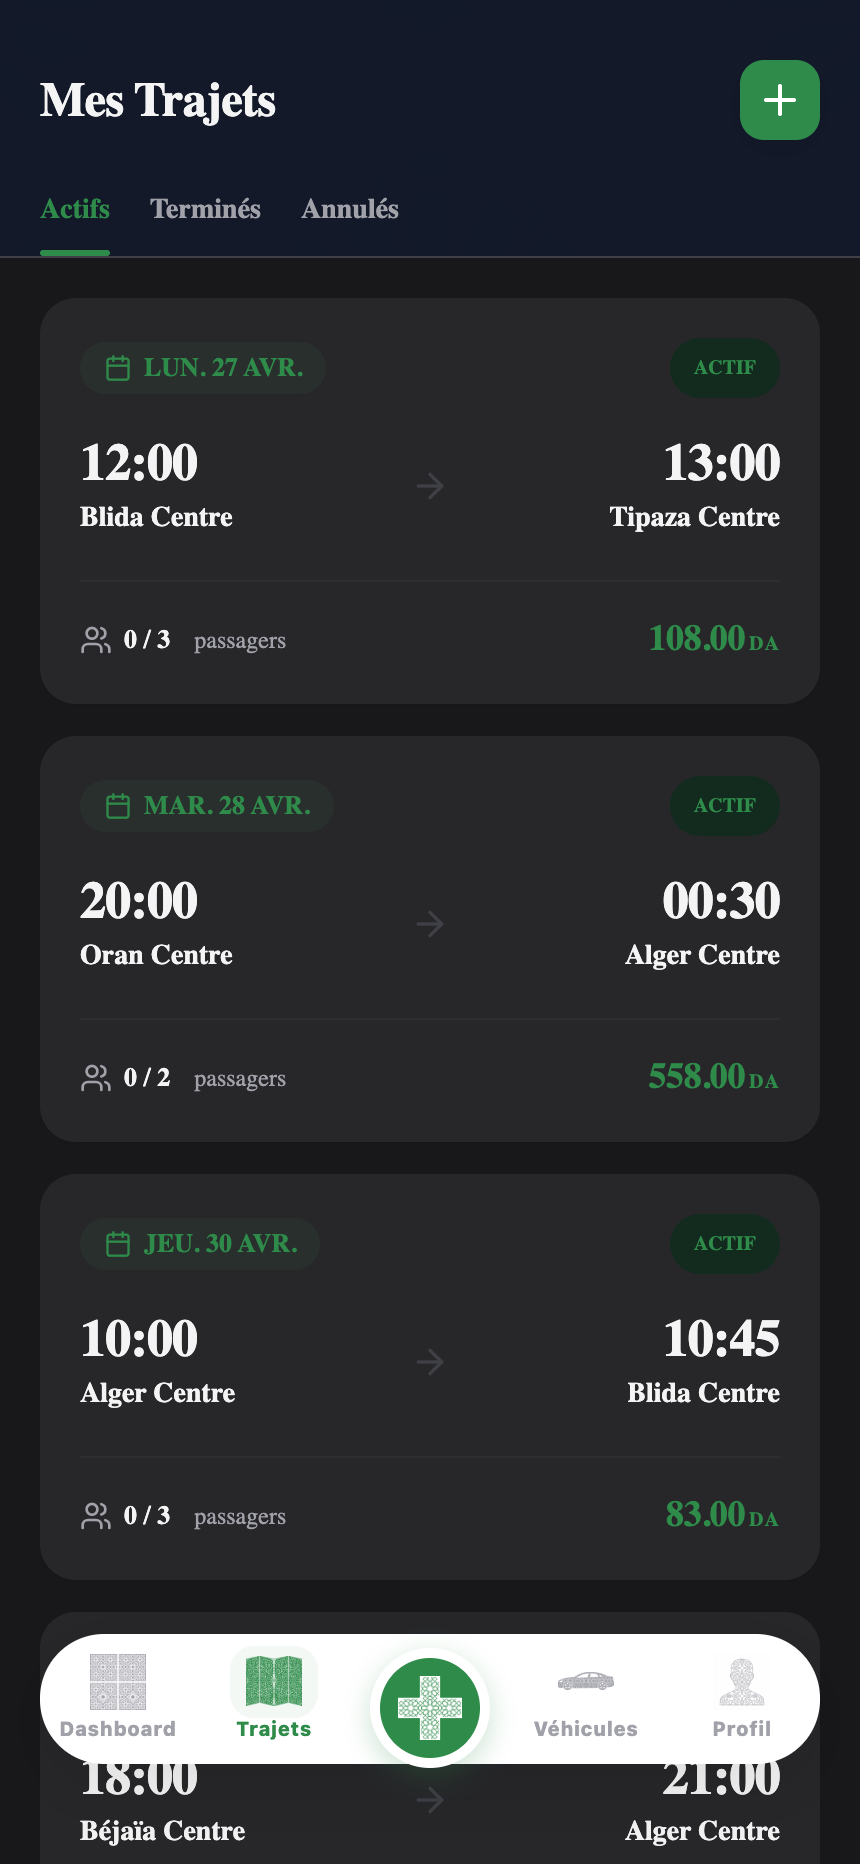
\includegraphics[width=\linewidth]{mobile-all/d_02_tab_trips.png}
    {\footnotesize \textbf{3.9a} --- Mes trajets (conducteur)\\Trajets actifs, passés, annulés.\par}
\end{minipage}\hfill
\begin{minipage}{0.31\textwidth}
    \centering
    
\includegraphics[width=\linewidth]{mobile-all/d_12_trip_requests.png}
    {\footnotesize \textbf{3.9b} --- Demandes de trajet\\\textit{Matching} inverse vers conducteur.\par}
\end{minipage}\hfill
\begin{minipage}{0.31\textwidth}
    \centering
    
\includegraphics[width=\linewidth]{mobile-all/d_07_earnings.png}
    {\footnotesize \textbf{3.9c} --- Gains du mois\\Récapitulatif par trajet, courbe de revenus.\par}
\end{minipage}
\caption{Parcours conducteur --- trajets, demandes et gains}
\label{fig:driver-trips}
\end{figure}

\begin{figure}[H]
\centering
\begin{minipage}{0.31\textwidth}
    \centering
    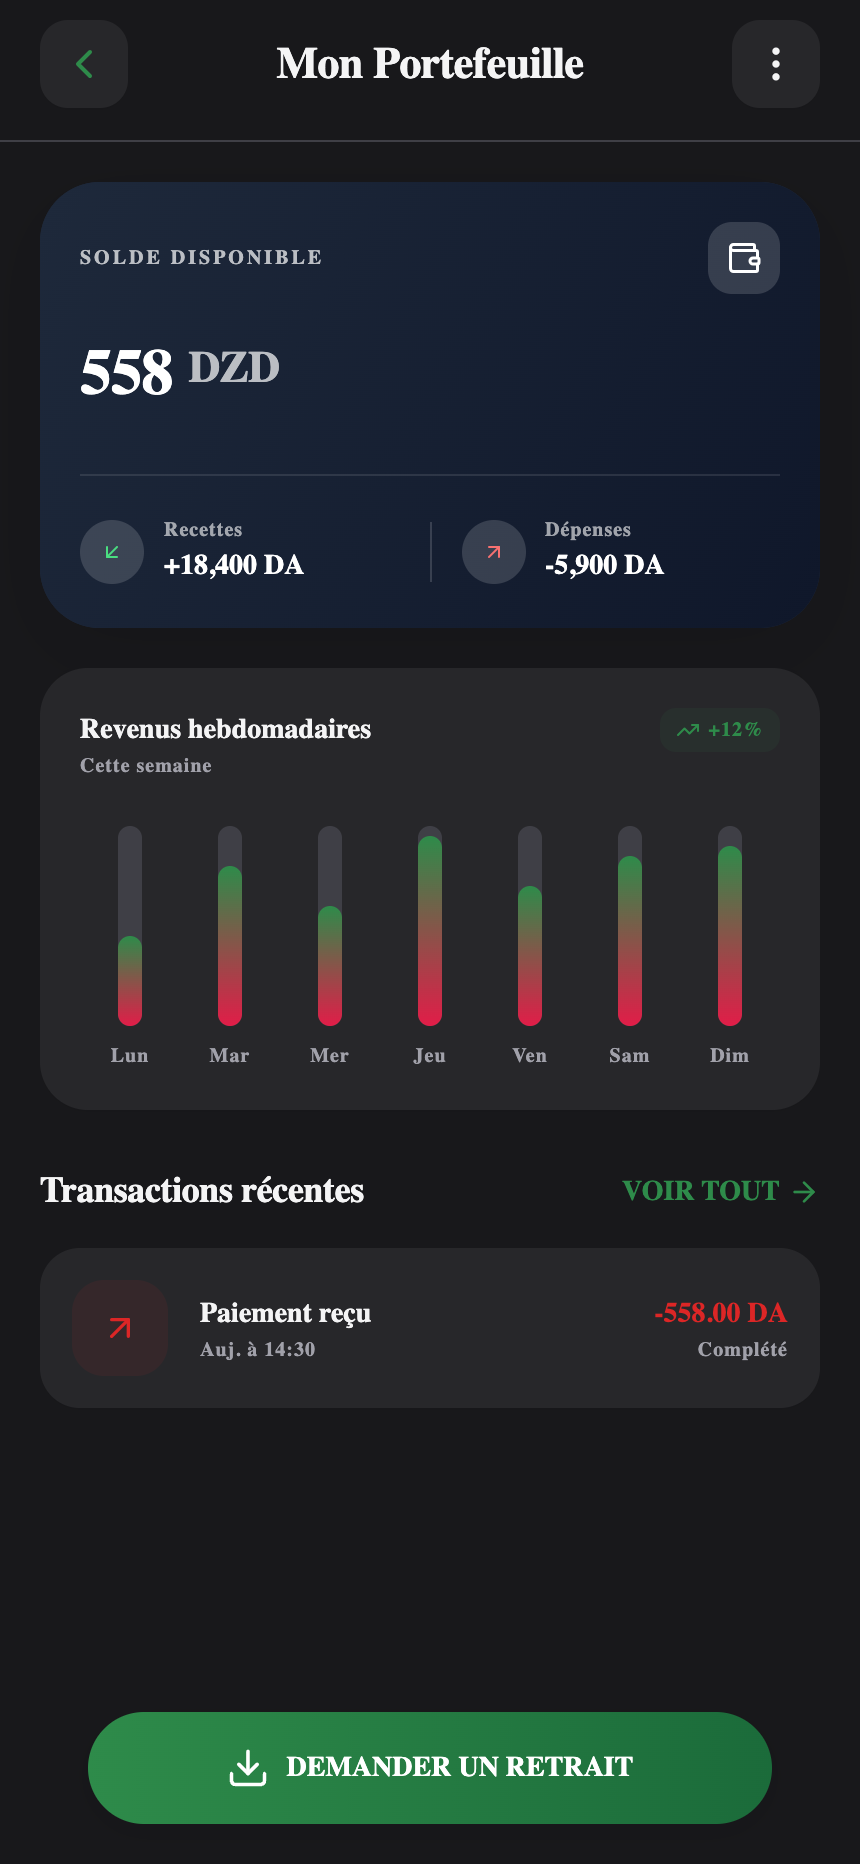
\includegraphics[width=\linewidth]{mobile-all/d_11_wallet.png}
    {\footnotesize \textbf{3.10a} --- Portefeuille conducteur\\Solde, historique, retrait bancaire.\par}
\end{minipage}\hfill
\begin{minipage}{0.31\textwidth}
    \centering
    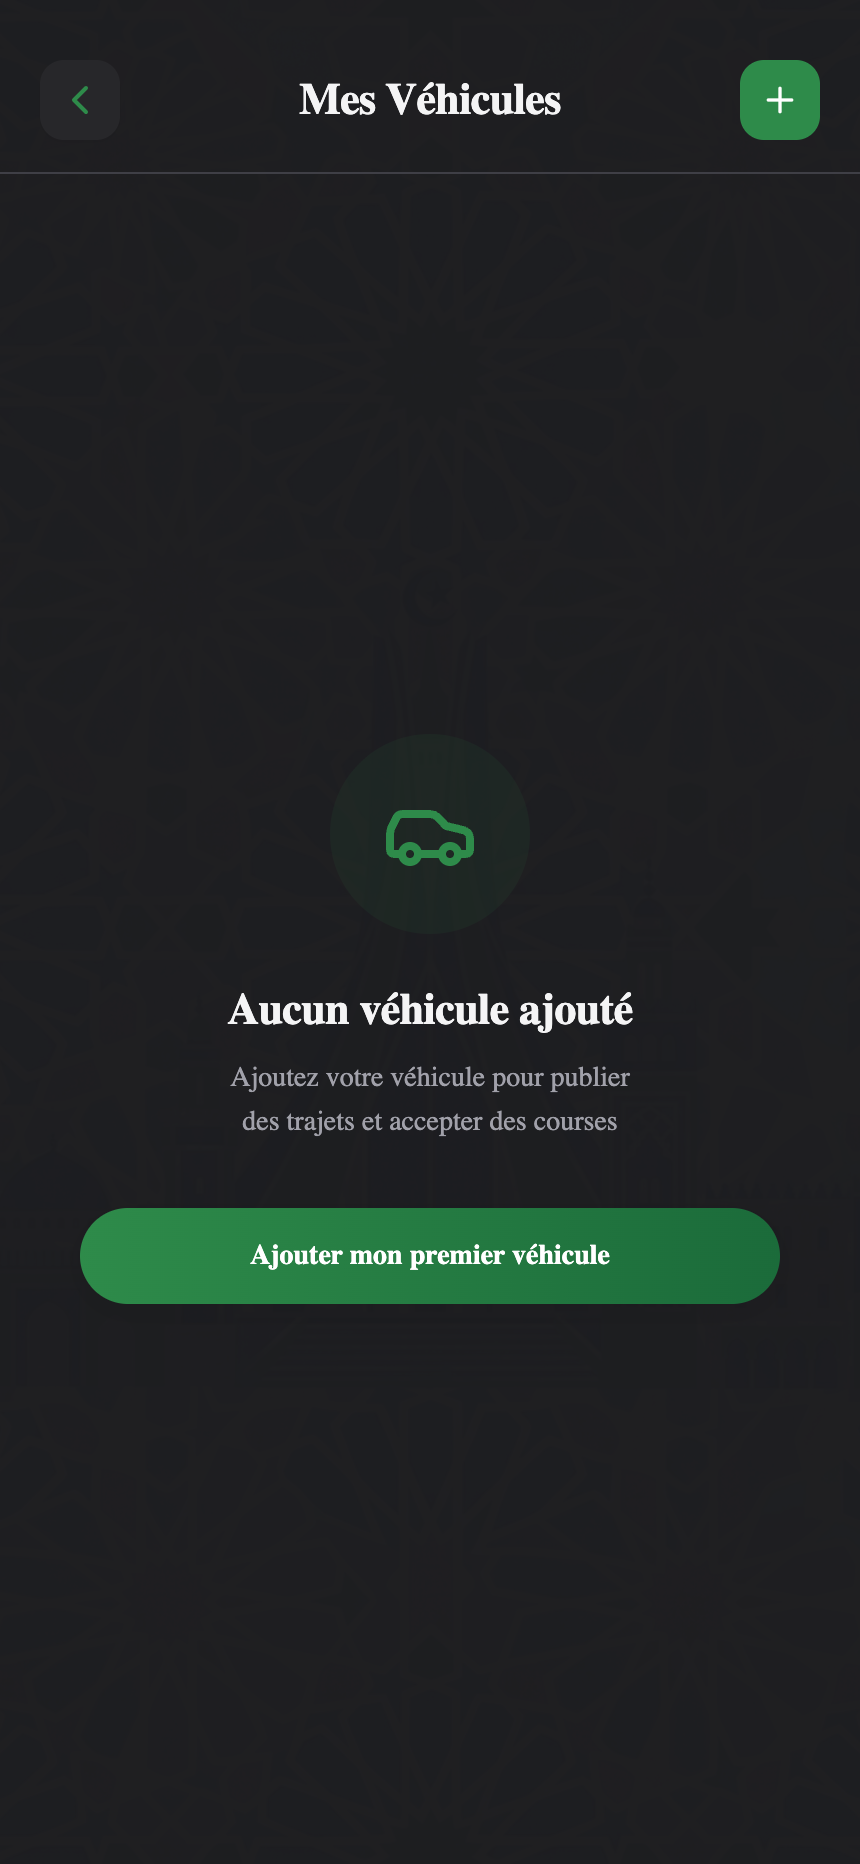
\includegraphics[width=\linewidth]{mobile-all/d_13_vehicles_list.png}
    {\footnotesize \textbf{3.10b} --- Liste des véhicules\\Véhicules enregistrés, sélection.\par}
\end{minipage}\hfill
\begin{minipage}{0.31\textwidth}
    \centering
    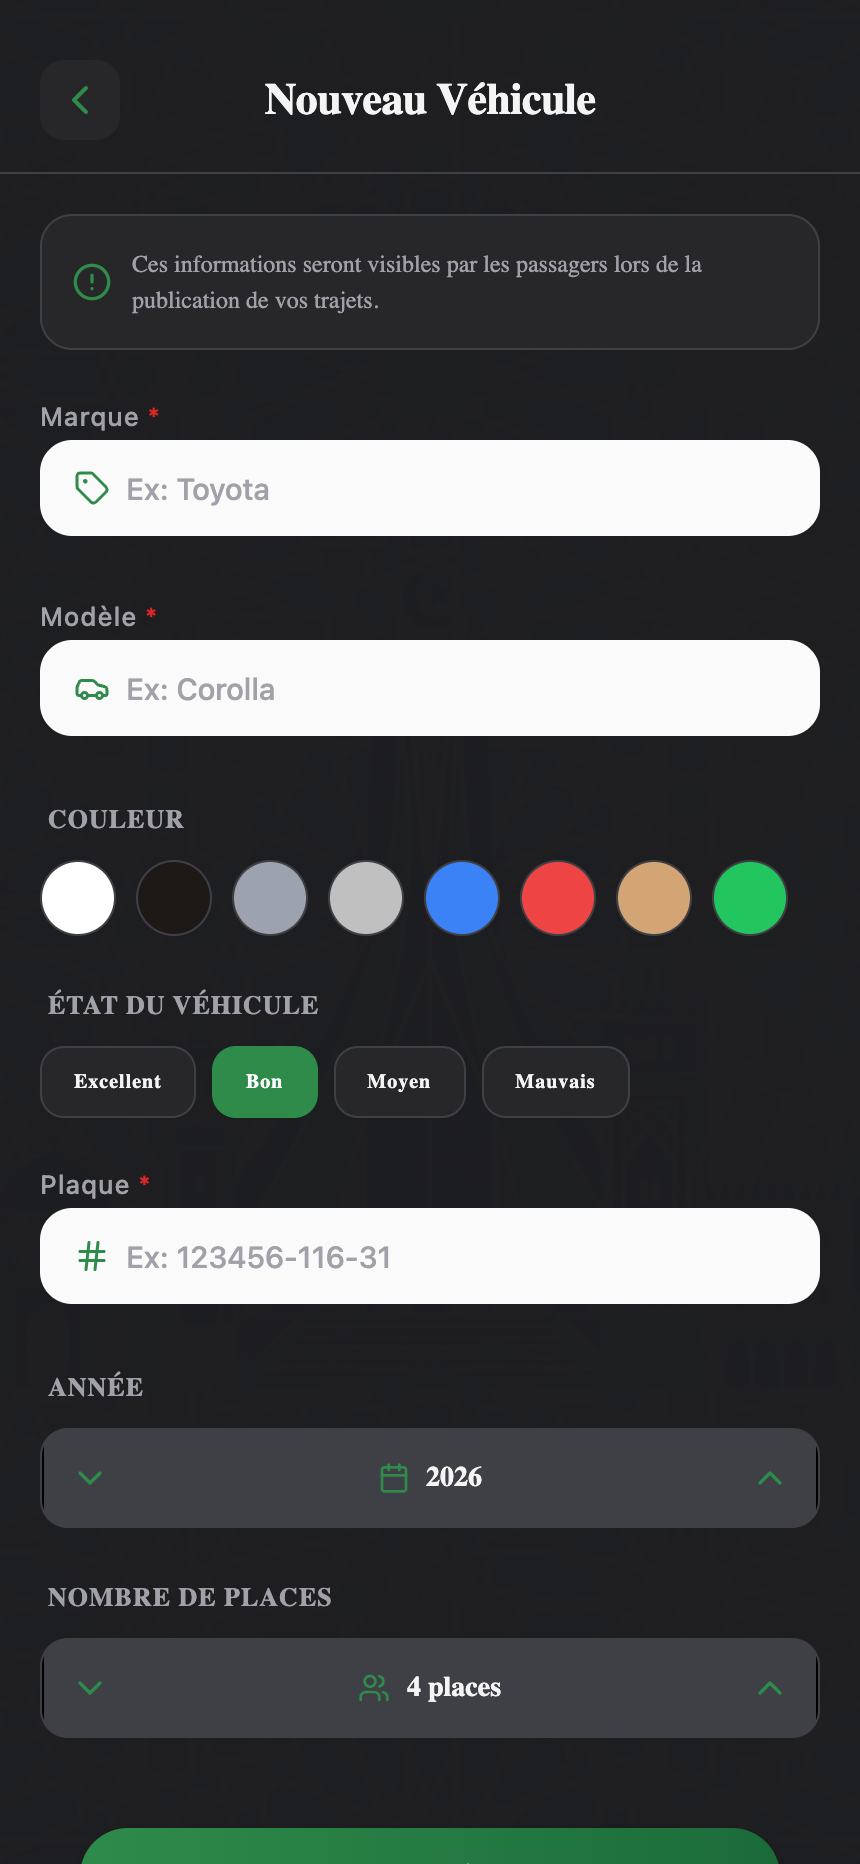
\includegraphics[width=\linewidth]{mobile-all/d_08_add_vehicle.png}
    {\footnotesize \textbf{3.10c} --- Ajout d'un véhicule\\Plaque chiffrée AES-256, places, marque.\par}
\end{minipage}
\caption{Parcours conducteur --- portefeuille et gestion des véhicules}
\label{fig:driver-wallet}
\end{figure}

\begin{figure}[H]
\centering
\begin{minipage}{0.31\textwidth}
    \centering
    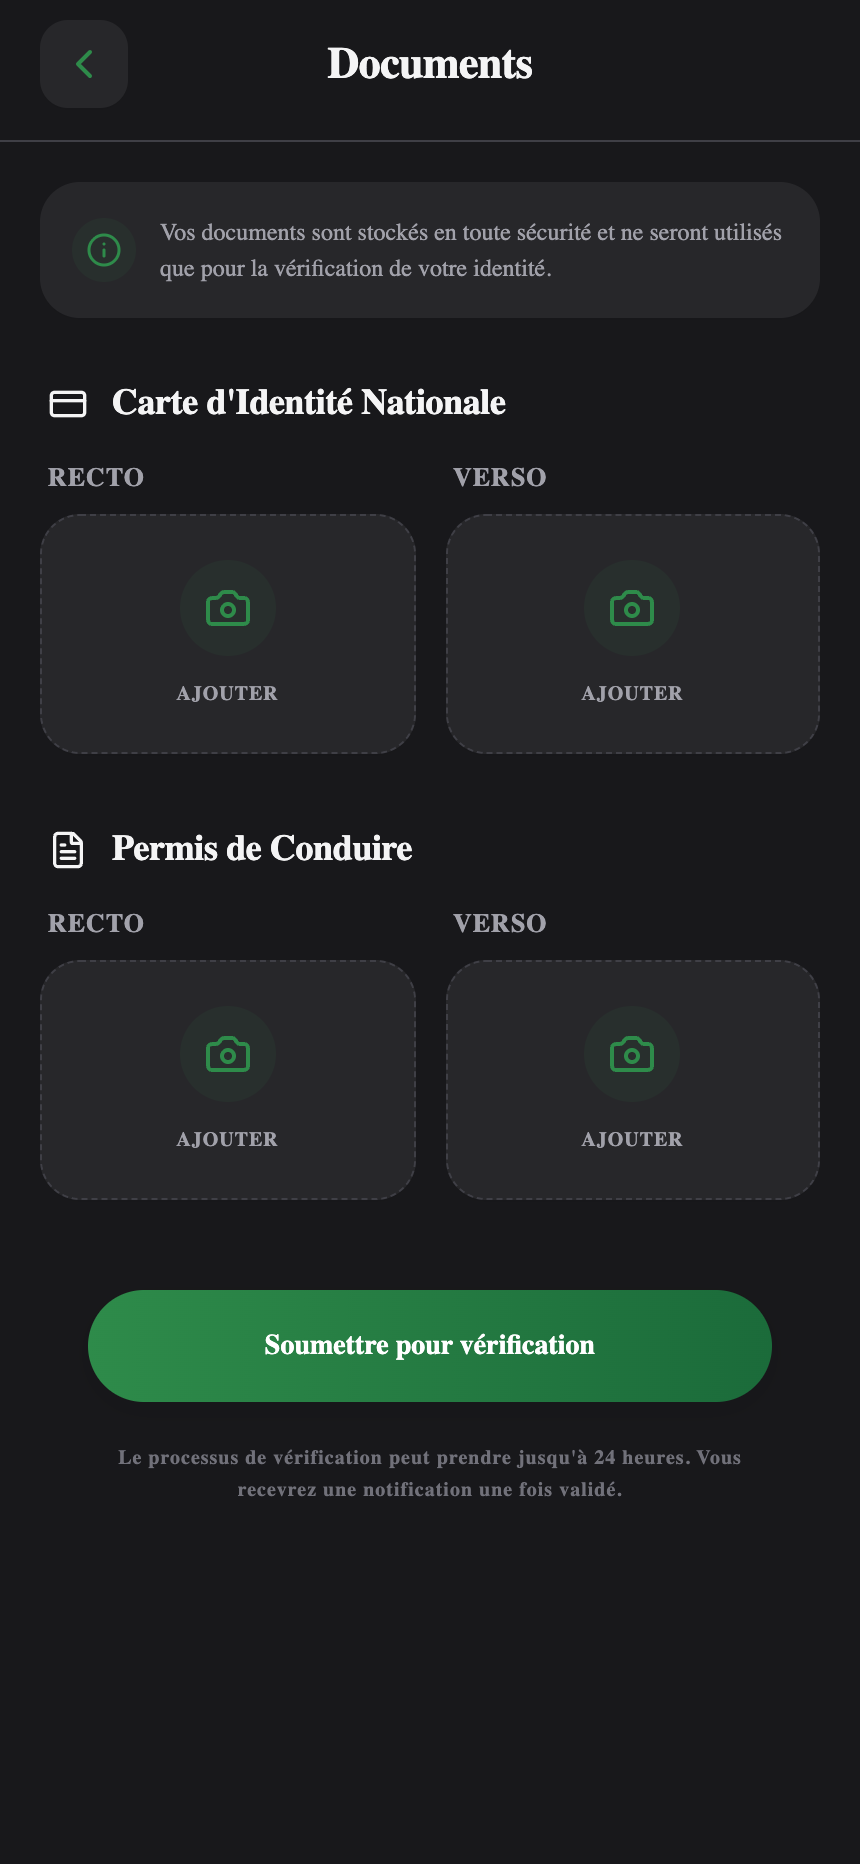
\includegraphics[width=\linewidth]{mobile-all/d_10_documents.png}
    {\footnotesize \textbf{3.11a} --- Documents du véhicule\\Assurance, carte grise, contrôle technique.\par}
\end{minipage}\hfill
\begin{minipage}{0.31\textwidth}
    \centering
    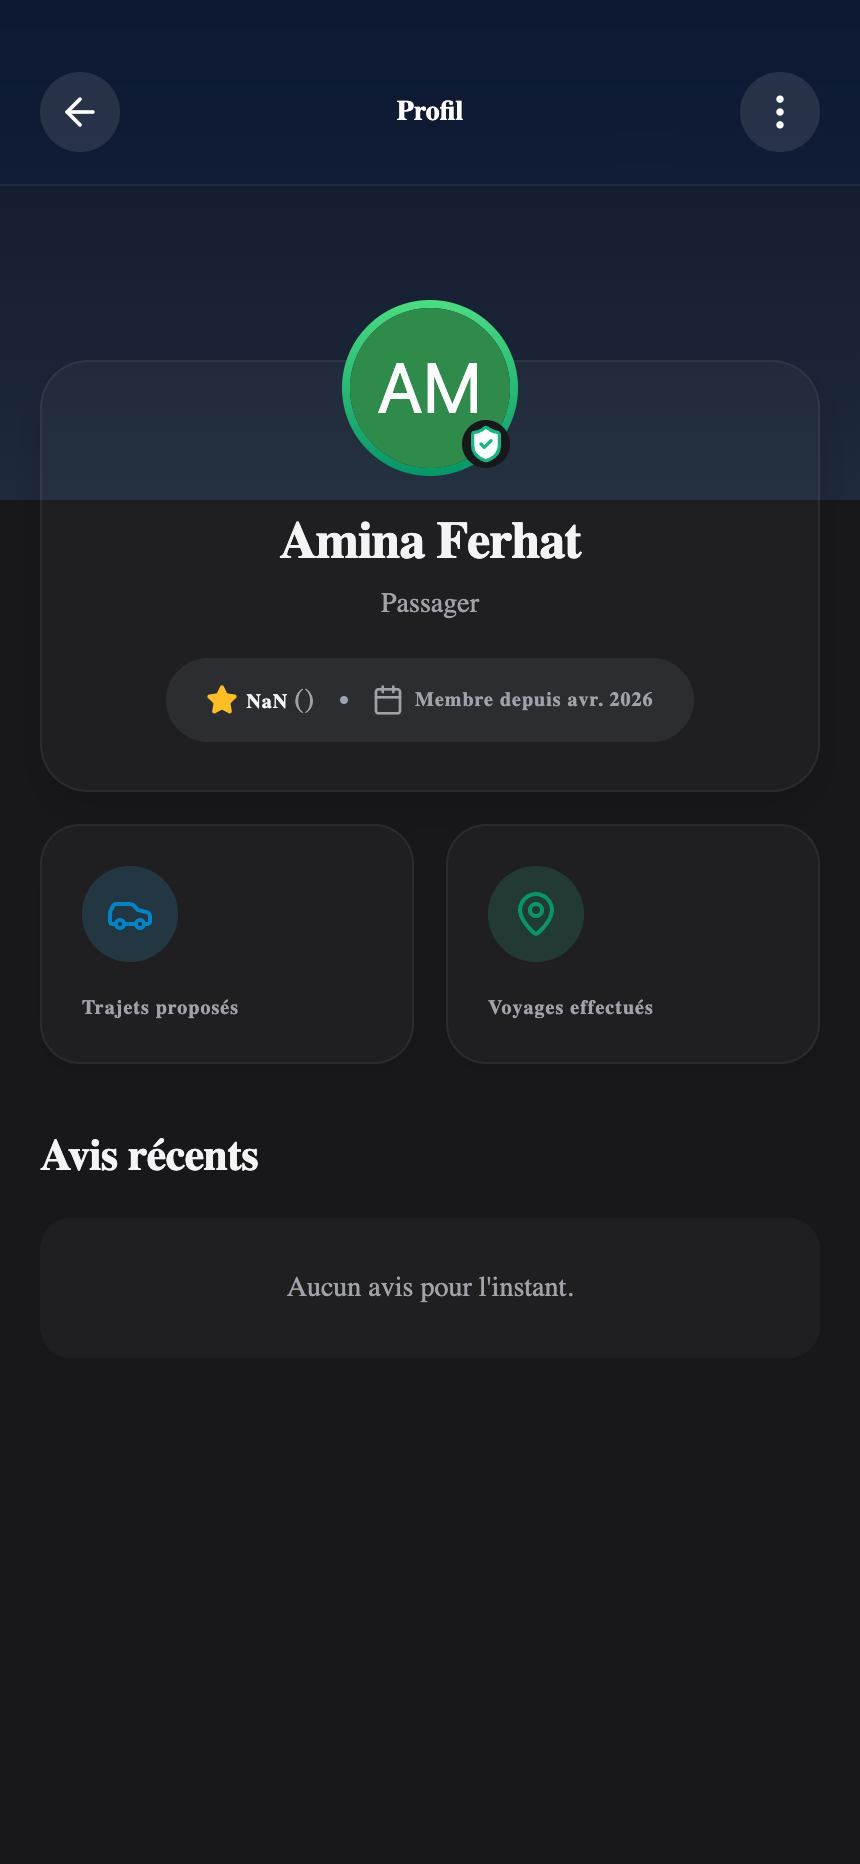
\includegraphics[width=\linewidth]{mobile-all/d_14_public_profile.png}
    {\footnotesize \textbf{3.11b} --- Profil public conducteur\\Note, trajets, véhicule, badge \textsc{kyc} Pro.\par}
\end{minipage}\hfill
\begin{minipage}{0.31\textwidth}
    \centering
    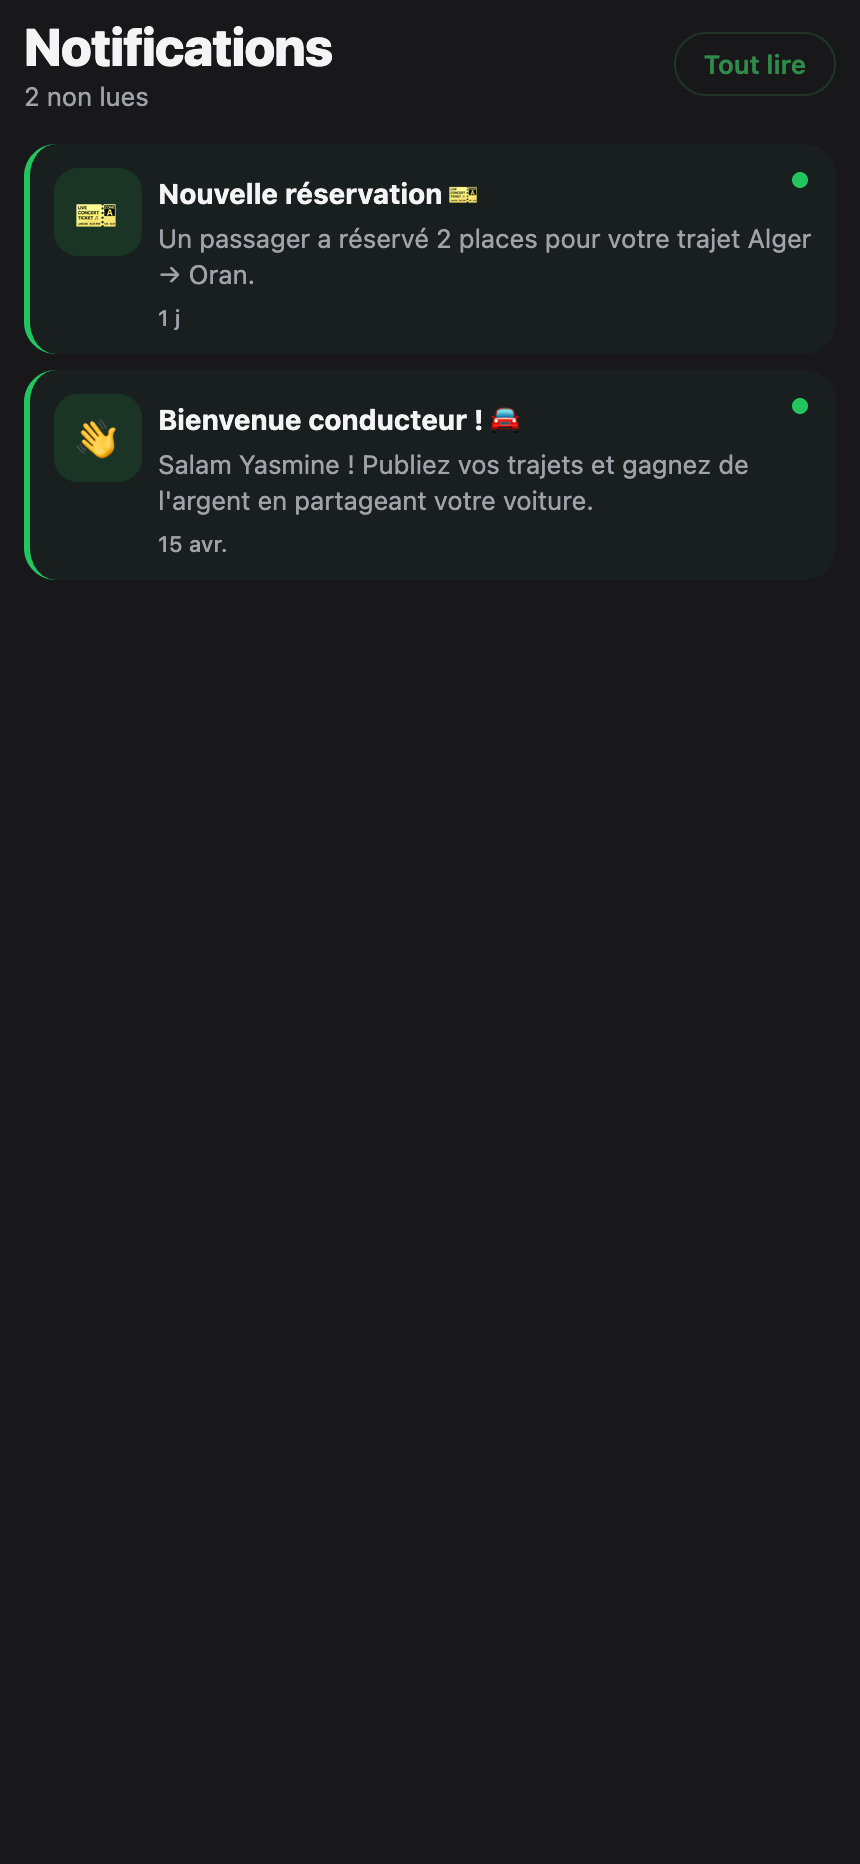
\includegraphics[width=\linewidth]{mobile-all/d_26_notifications.png}
    {\footnotesize \textbf{3.11c} --- Notifications\\Réservations, confirmations, alertes admin.\par}
\end{minipage}
\caption{Parcours conducteur --- documents, profil et notifications}
\label{fig:driver-docs}
\end{figure}

\subsection{Profil et paramètres (commun passager / conducteur)}

Les écrans de profil et de paramètres sont partagés entre les deux rôles. Ils permettent à l'utilisateur de gérer son identité, sa sécurité, ses préférences et d'accéder au support.

\begin{figure}[H]
\centering
\begin{minipage}{0.31\textwidth}
    \centering
    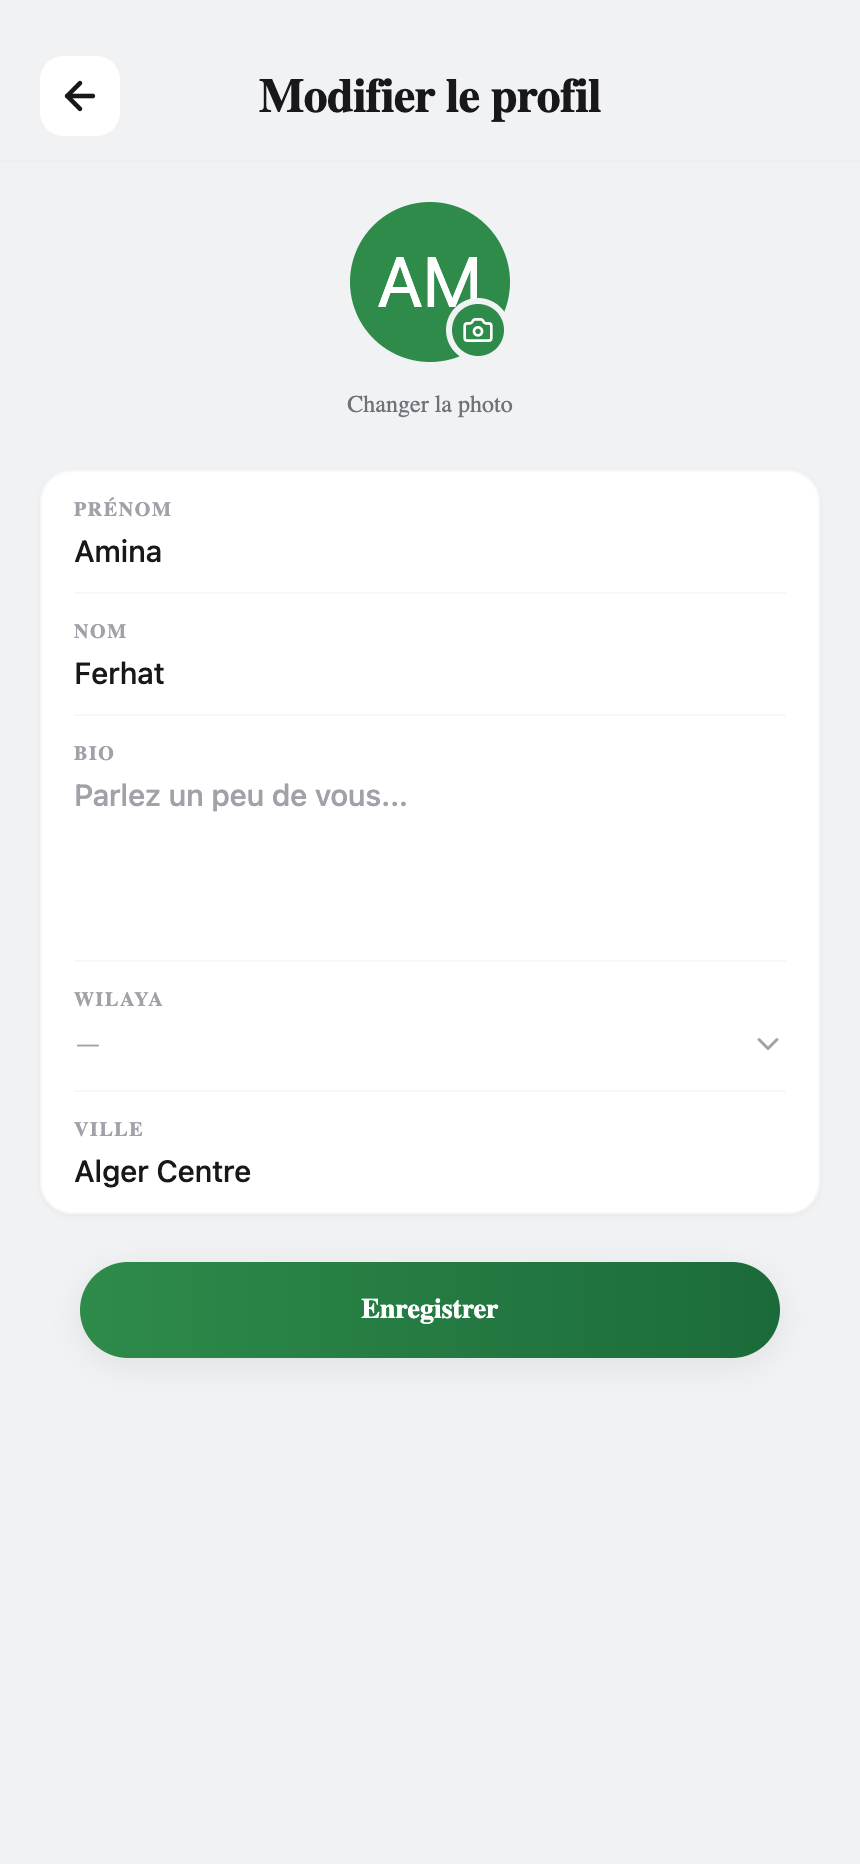
\includegraphics[width=\linewidth]{mobile-all/p_14_edit_profile.png}
    {\footnotesize \textbf{3.12a} --- Modifier mon profil\\Nom, photo, wilaya, droit de rectification.\par}
\end{minipage}\hfill
\begin{minipage}{0.31\textwidth}
    \centering
    
\includegraphics[width=\linewidth]{mobile-all/p_18_security_phone.png}
    {\footnotesize \textbf{3.12b} --- Sécurité du compte\\Numéro, sessions actives, déconnexion.\par}
\end{minipage}\hfill
\begin{minipage}{0.31\textwidth}
    \centering
    
\includegraphics[width=\linewidth]{mobile-all/p_19_change_phone_otp.png}
    {\footnotesize \textbf{3.12c} --- Changement de numéro OTP\\Vérification \textsc{sms} avant mise à jour.\par}
\end{minipage}
\caption{Profil et sécurité du compte}
\label{fig:profile-security}
\end{figure}

\begin{figure}[H]
\centering
\begin{minipage}{0.31\textwidth}
    \centering
    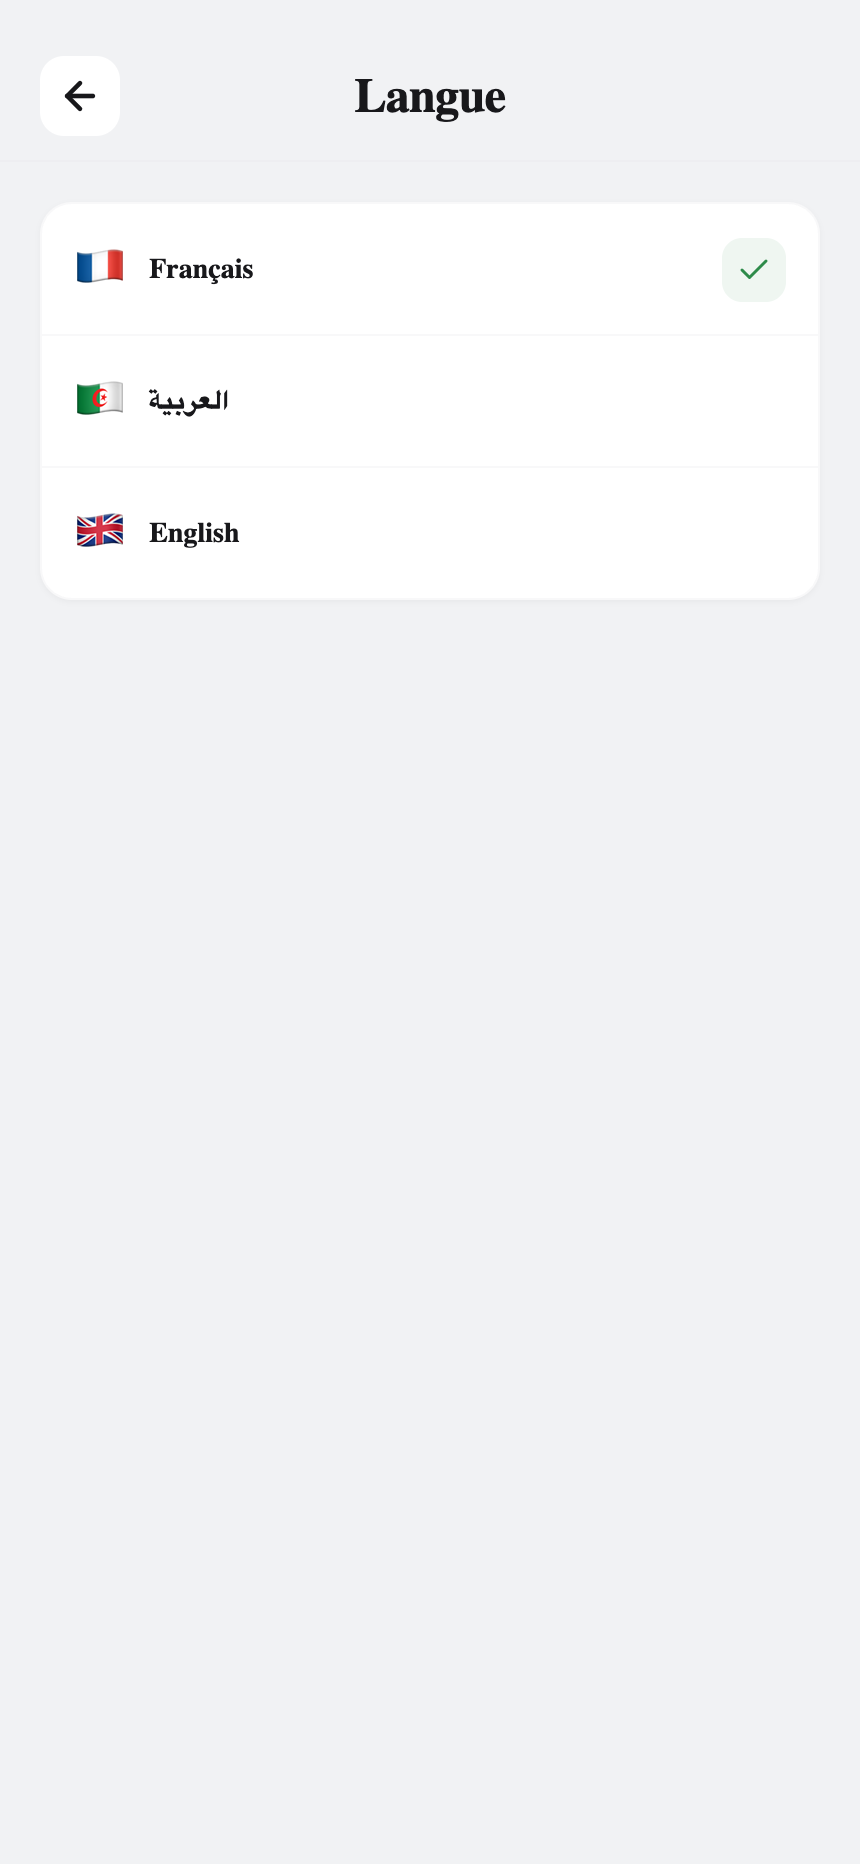
\includegraphics[width=\linewidth]{mobile-all/p_20_language_select.png}
    {\footnotesize \textbf{3.13a} --- Sélection de la langue\\Arabe (RTL), français, anglais via i18next.\par}
\end{minipage}\hfill
\begin{minipage}{0.31\textwidth}
    \centering
    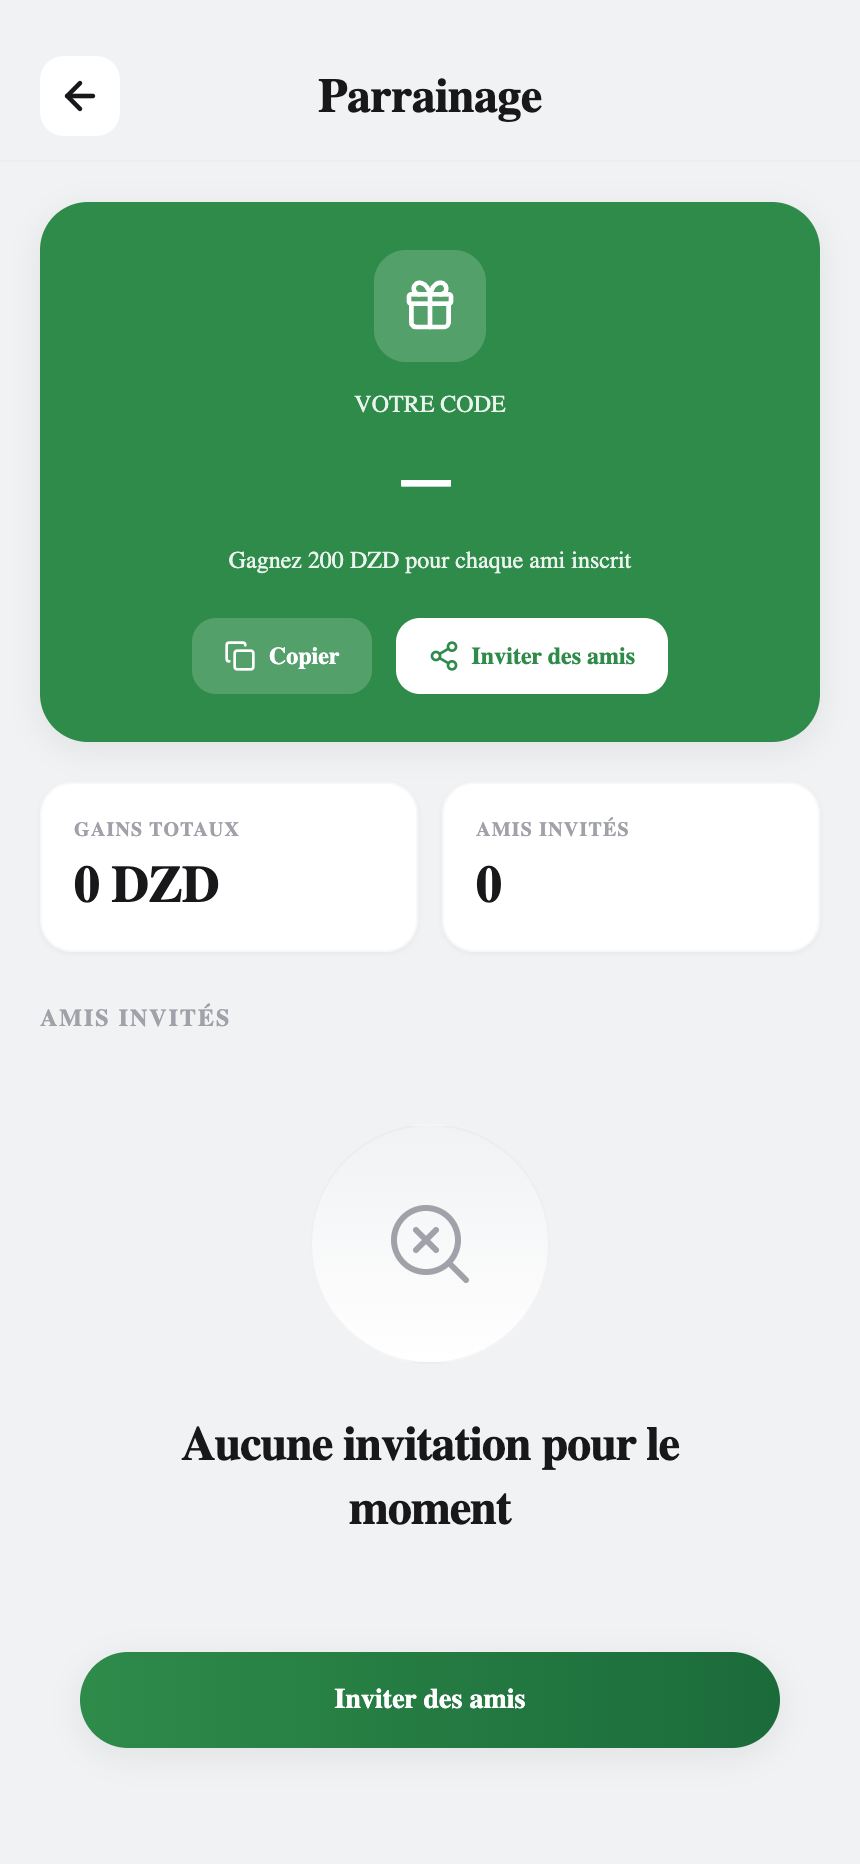
\includegraphics[width=\linewidth]{mobile-all/p_21_referral.png}
    {\footnotesize \textbf{3.13b} --- Programme de parrainage\\Code unique, crédit 200~DZD par parrainé.\par}
\end{minipage}\hfill
\begin{minipage}{0.31\textwidth}
    \centering
    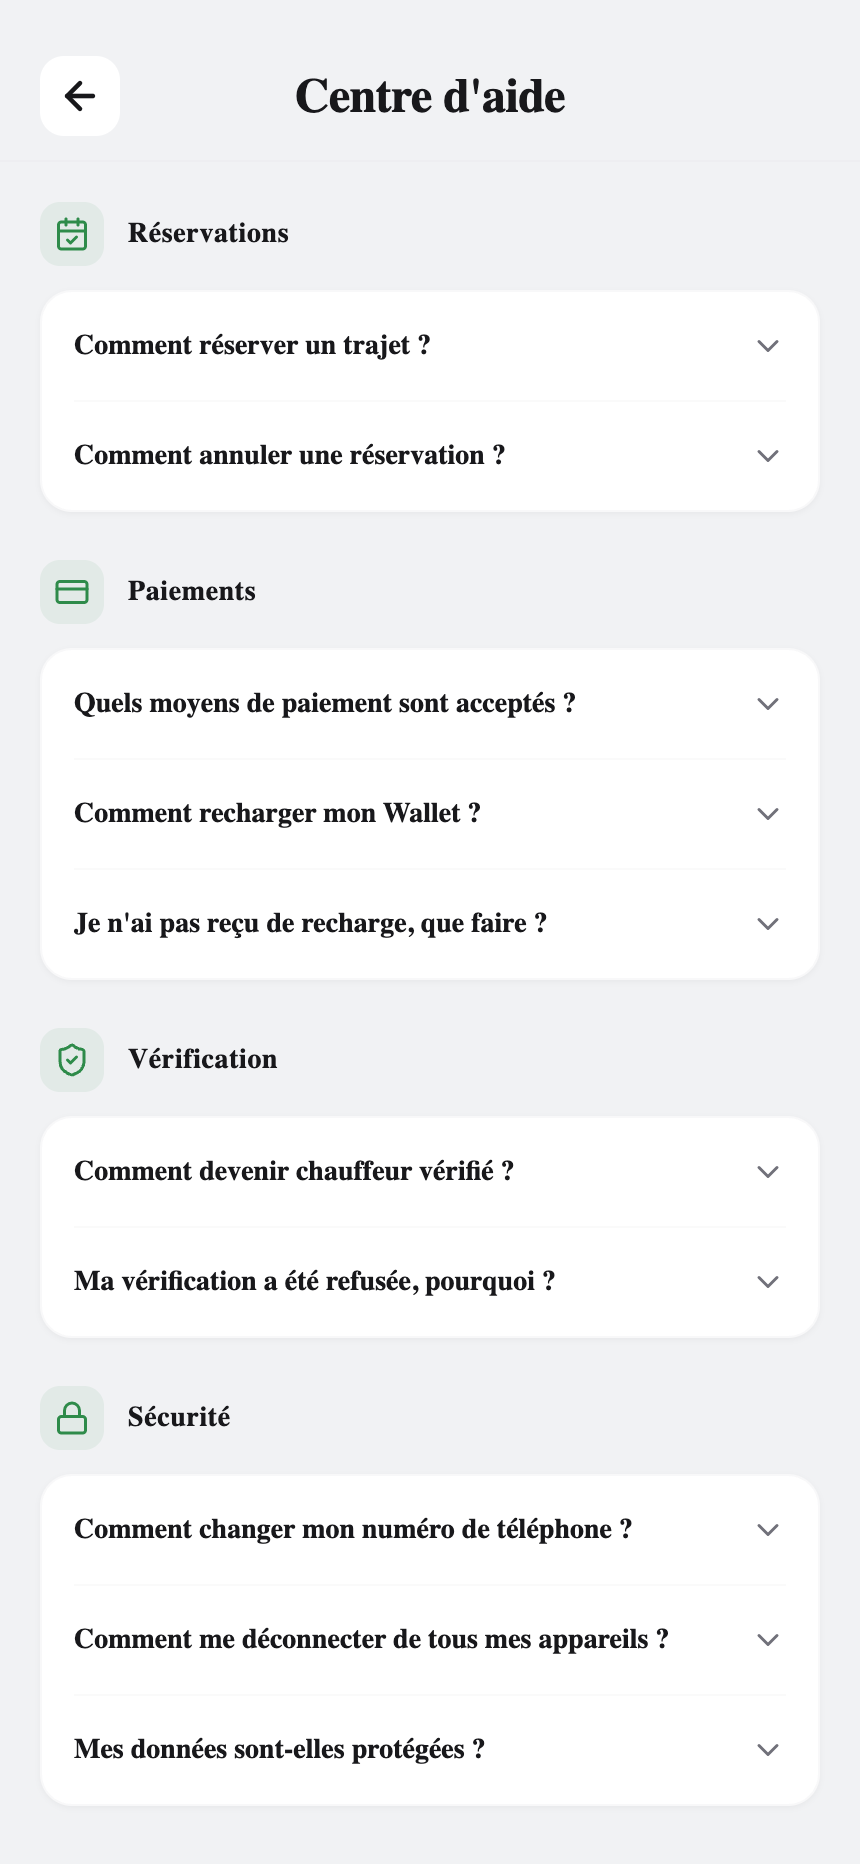
\includegraphics[width=\linewidth]{mobile-all/p_22_help_center.png}
    {\footnotesize \textbf{3.13c} --- Centre d'aide\\FAQ, signalement, support multicanal.\par}
\end{minipage}
\caption{Paramètres --- langue, parrainage et aide}
\label{fig:settings-lang}
\end{figure}

\begin{figure}[H]
\centering
\begin{minipage}{0.31\textwidth}
    \centering
    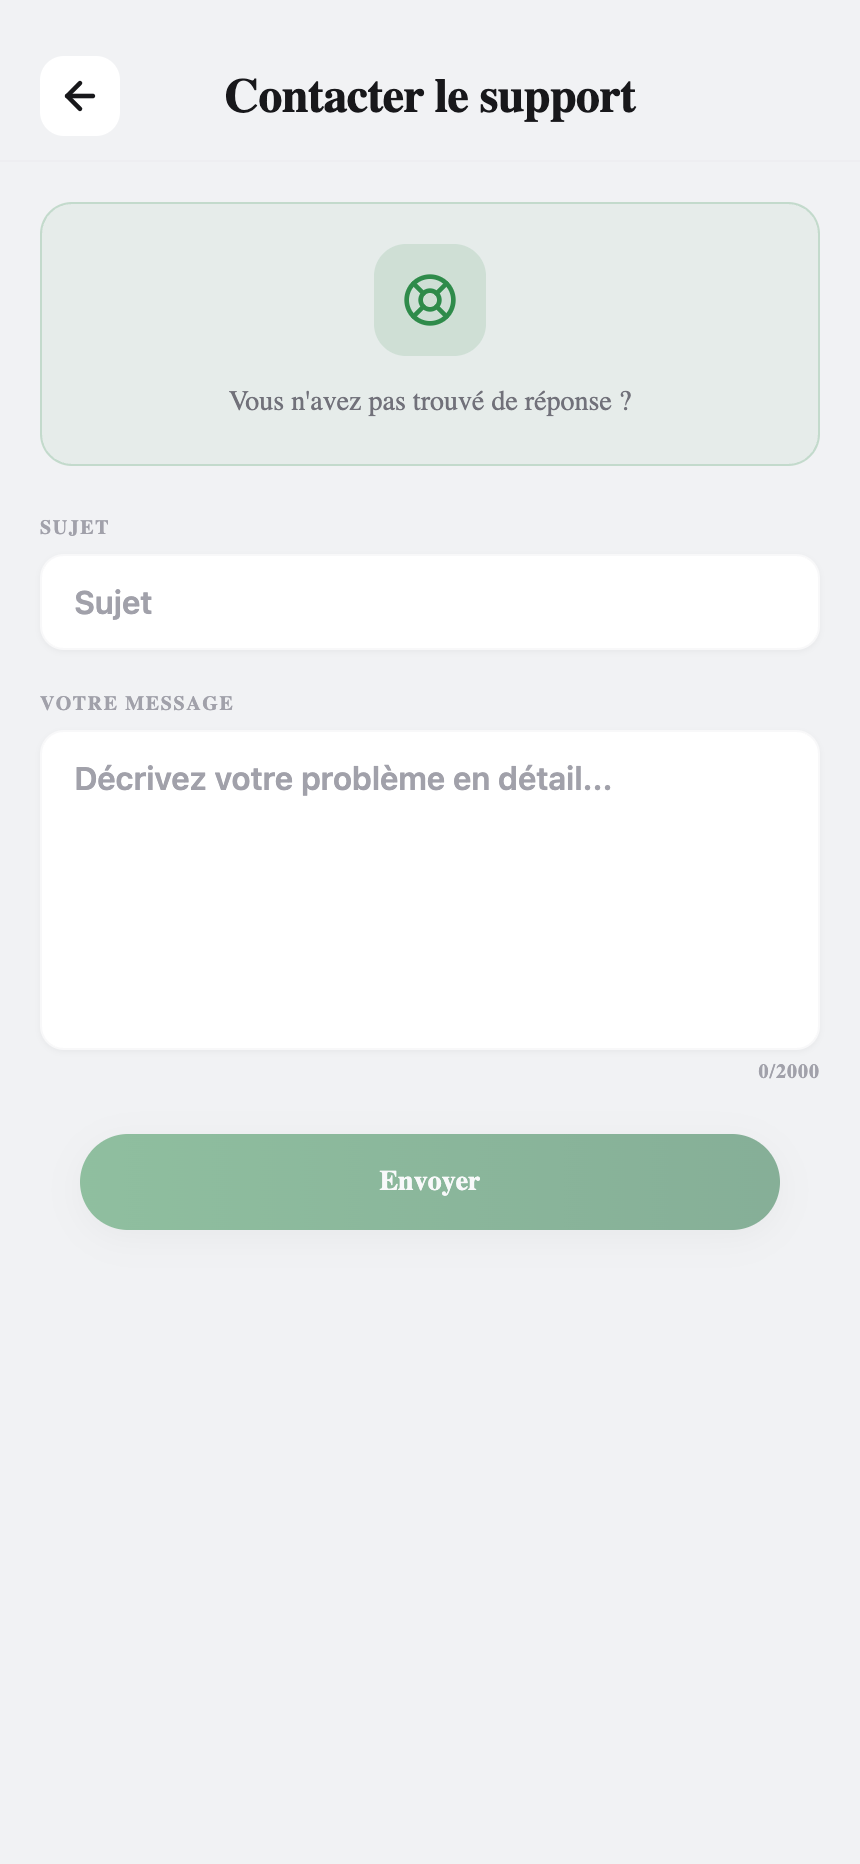
\includegraphics[width=\linewidth]{mobile-all/p_23_contact_support.png}
    {\footnotesize \textbf{3.14a} --- Contacter le support\\Chat en direct, email, formulaire de litige.\par}
\end{minipage}\hfill
\begin{minipage}{0.31\textwidth}
    \centering
    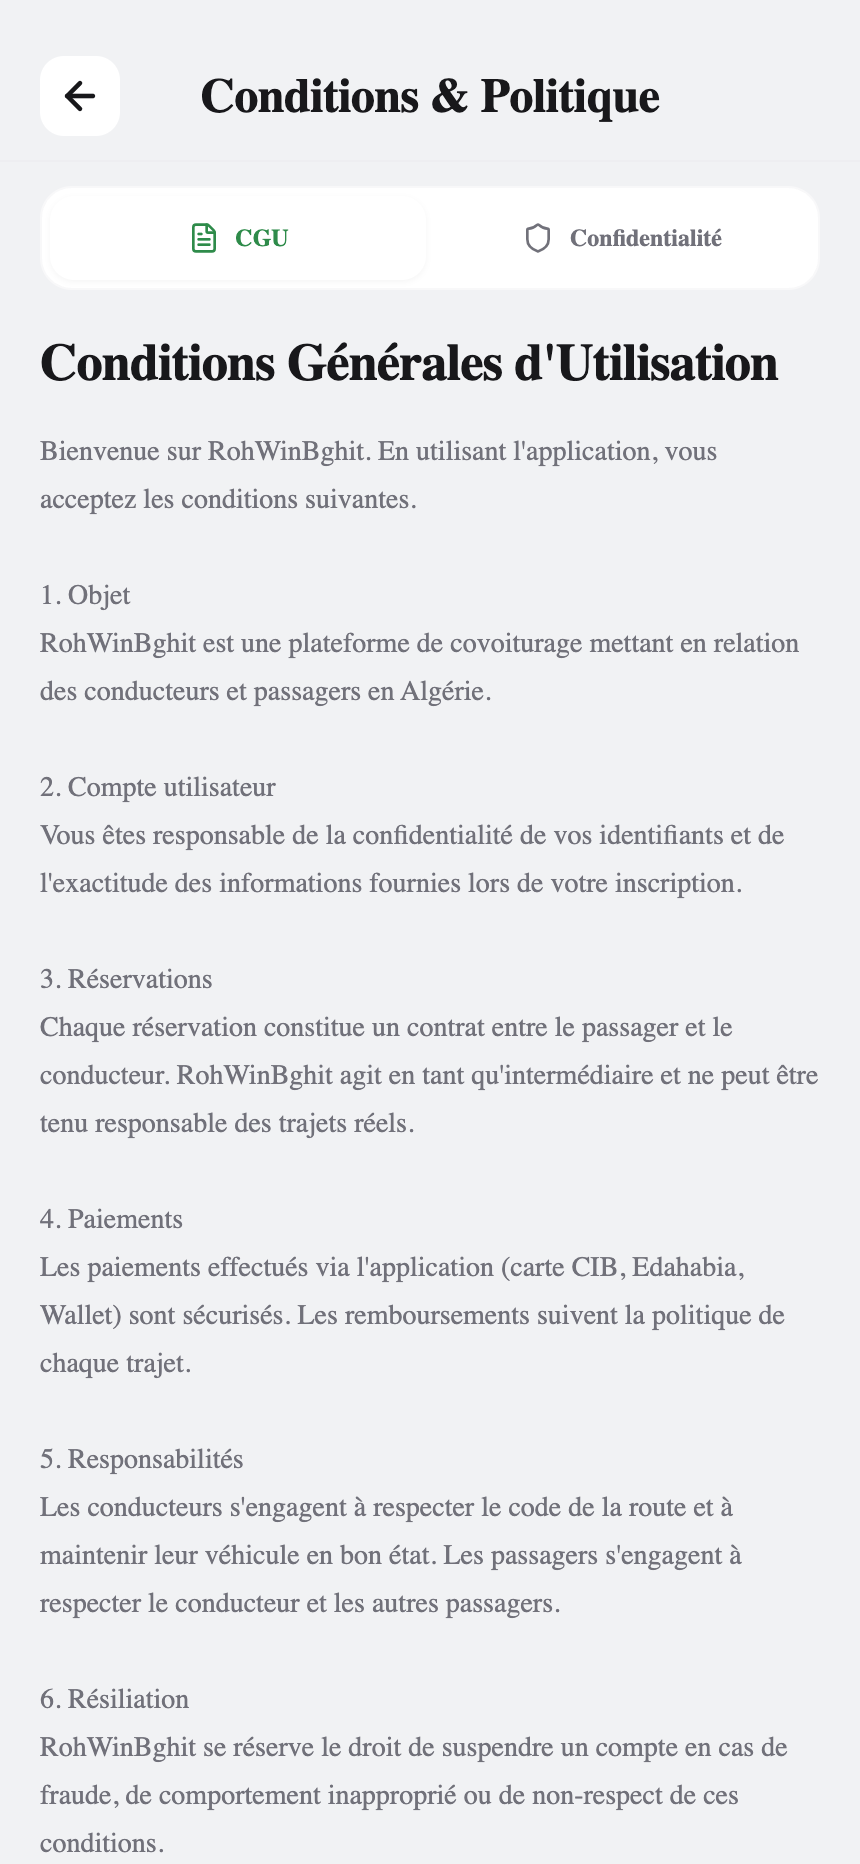
\includegraphics[width=\linewidth]{mobile-all/p_24_terms_legal.png}
    {\footnotesize \textbf{3.14b} --- Conditions générales\\CGU, politique conformité Loi~25-11.\par}
\end{minipage}\hfill
\begin{minipage}{0.31\textwidth}
    \centering
    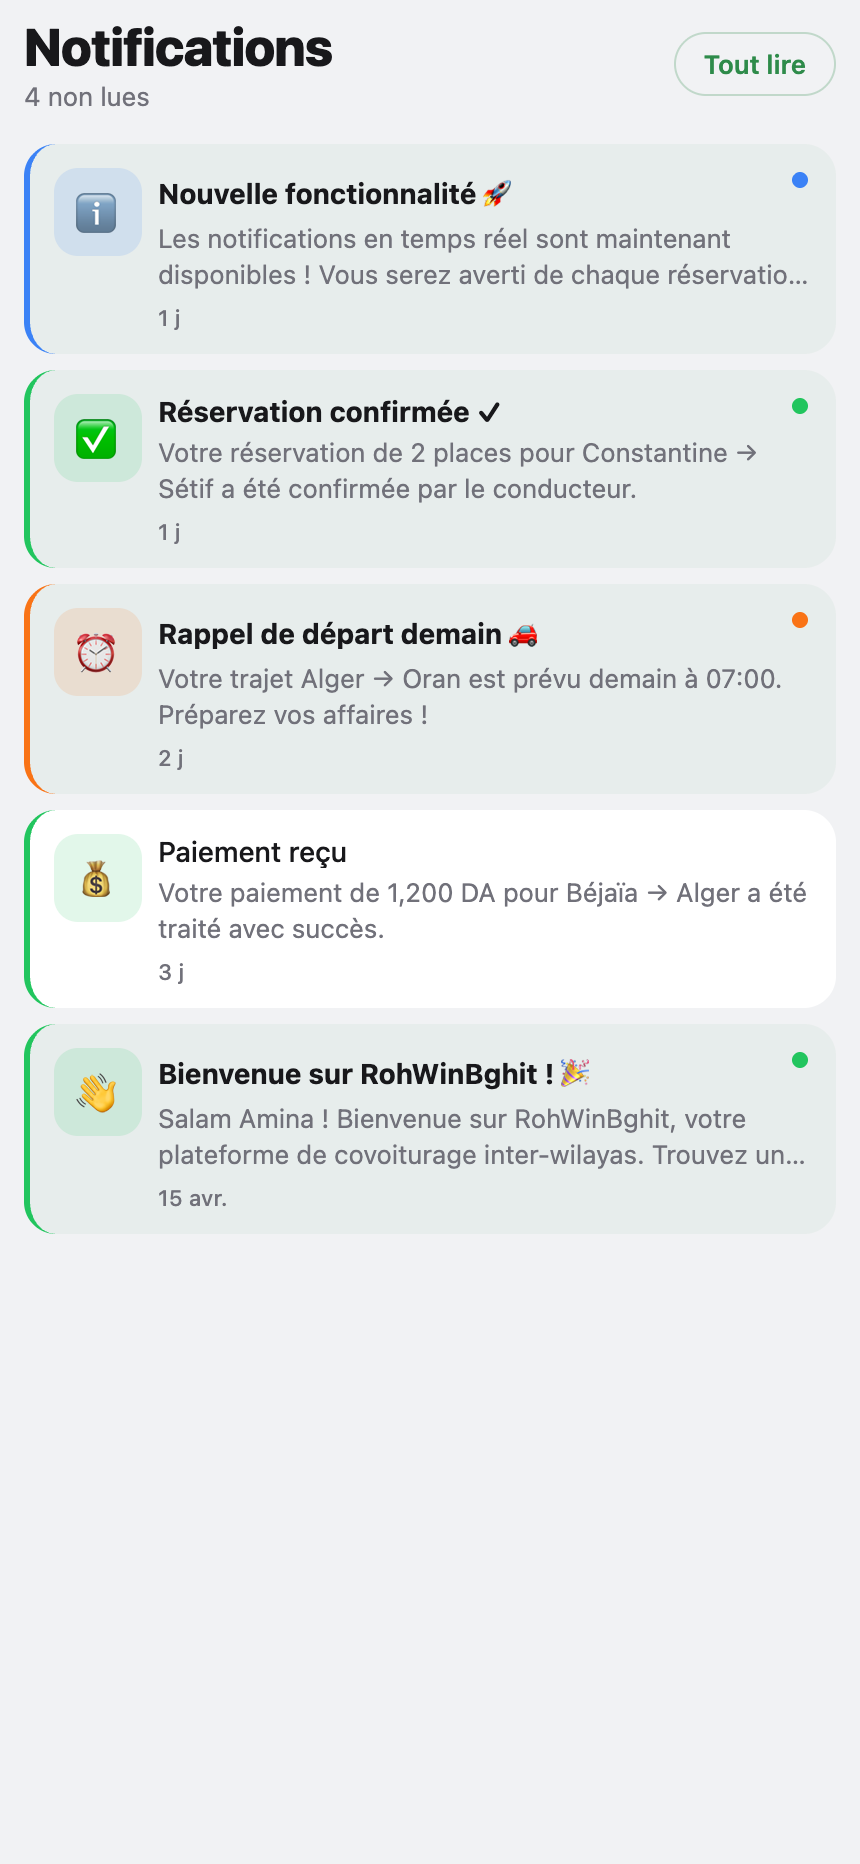
\includegraphics[width=\linewidth]{mobile-all/p_25_notifications.png}
    {\footnotesize \textbf{3.14c} --- Préférences de notification\\Contrôle granulaire \textit{push}/email.\par}
\end{minipage}
\caption{Paramètres --- support, mentions légales et notifications}
\label{fig:settings-legal}
\end{figure}

\section{Réalisation du tableau de bord administrateur}
\label{sec:realisation-admin}

Le panneau d'administration est développé avec React~+~Vite et déployé séparément. Il offre à l'opérateur une vision consolidée de la plateforme~: indicateurs clés, modération, revue \textsc{kyc}, supervision des trajets et analyse financière.

\begin{figure}[H]
\centering
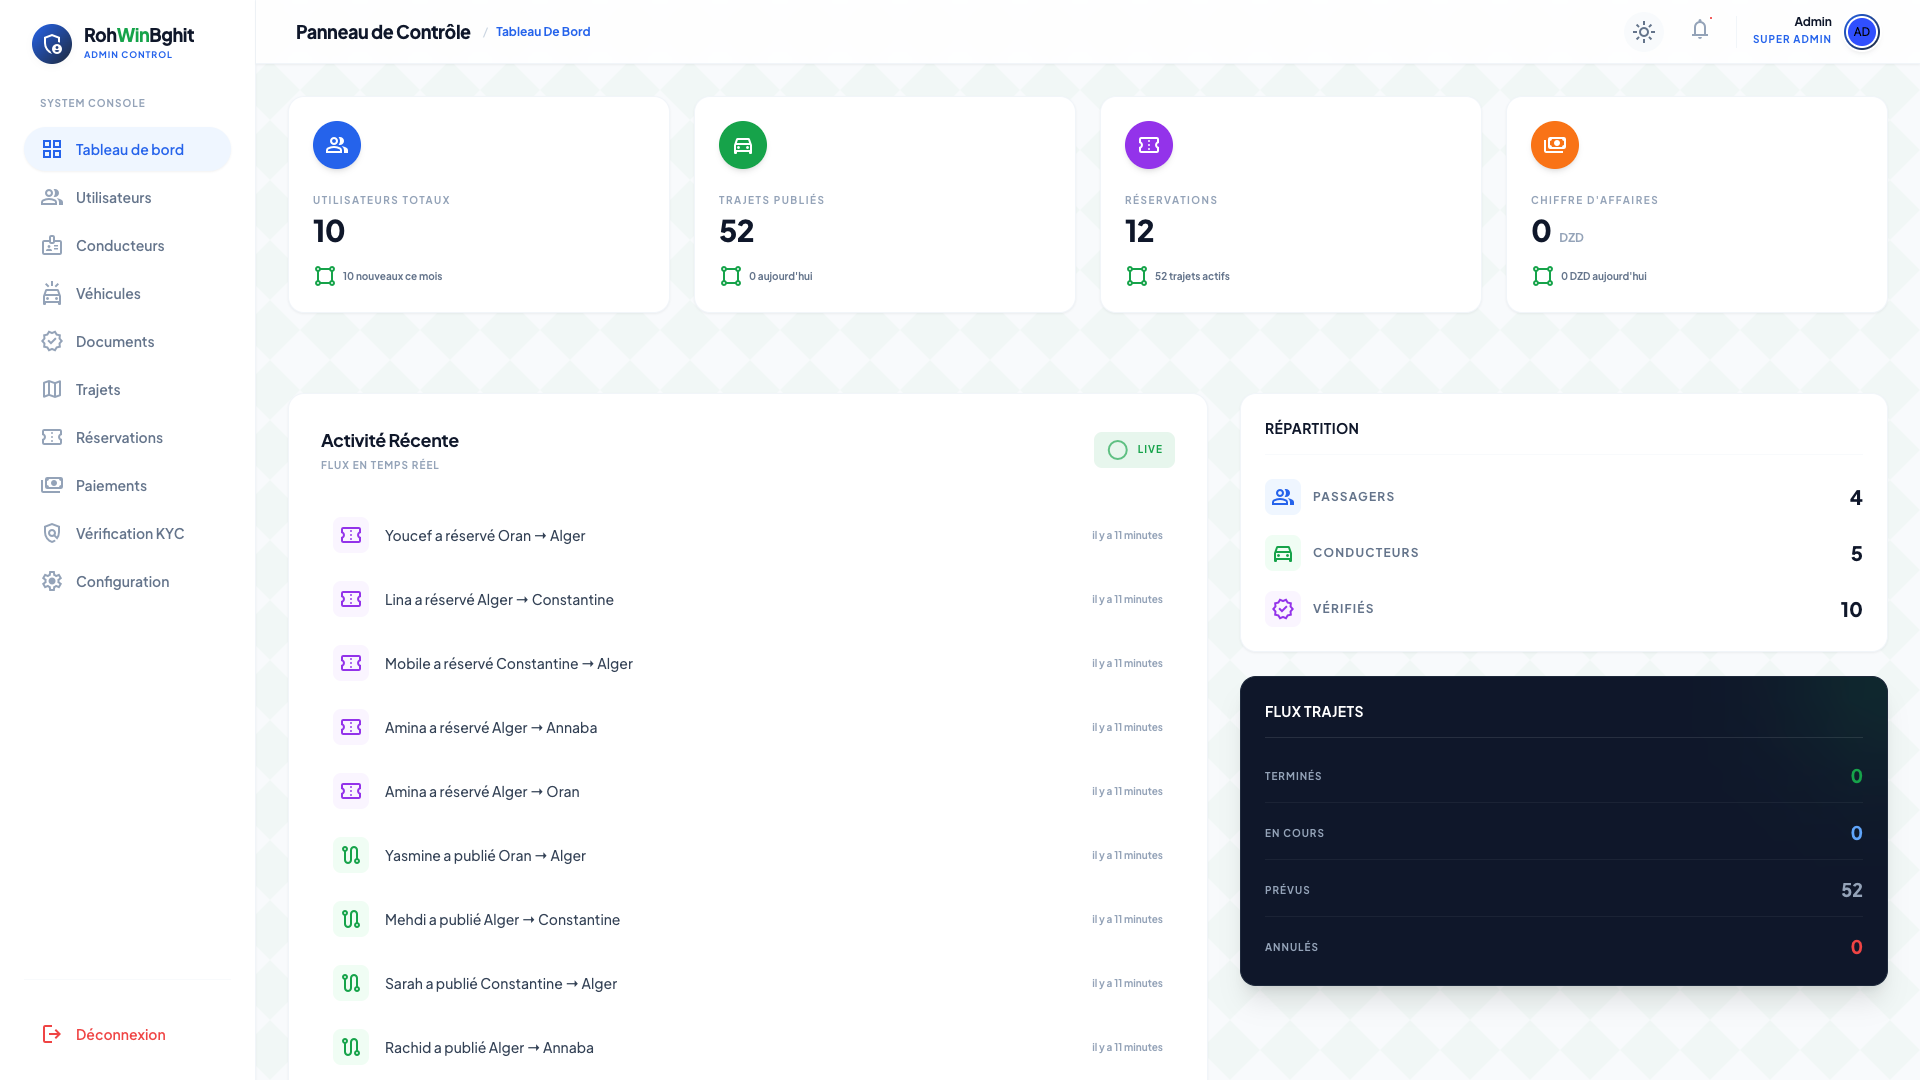
\includegraphics[width=0.95\linewidth]{assets/admin_dashboard.png}
\caption{Tableau de bord administrateur --- KPIs, graphiques et alertes en temps réel}
\label{fig:admin-dashboard}
\end{figure}

\begin{figure}[H]
\centering
\begin{minipage}{0.48\textwidth}
    \centering
    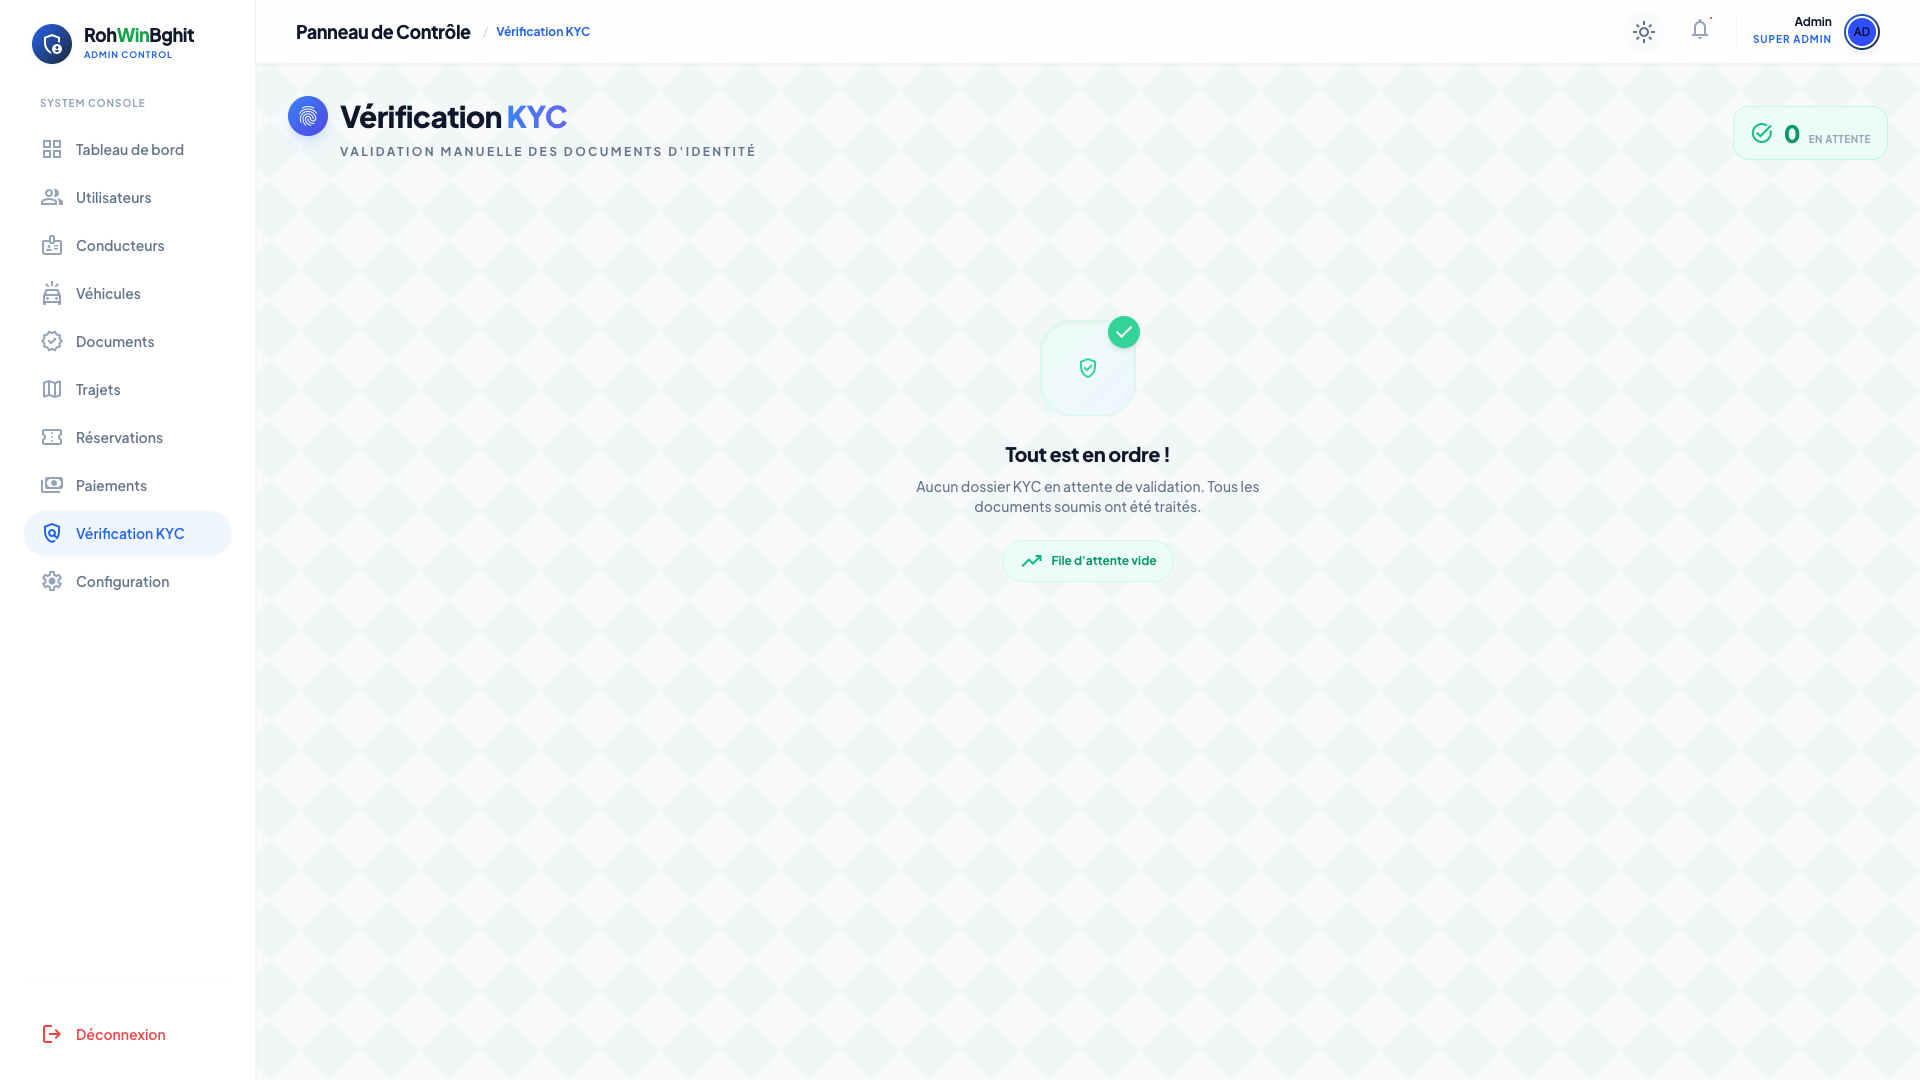
\includegraphics[width=\linewidth]{assets/admin_kyc.png}
    \caption{Revue manuelle des dossiers \textsc{kyc} litigieux}
    \label{fig:admin-kyc}
\end{minipage}\hfill
\begin{minipage}{0.48\textwidth}
    \centering
    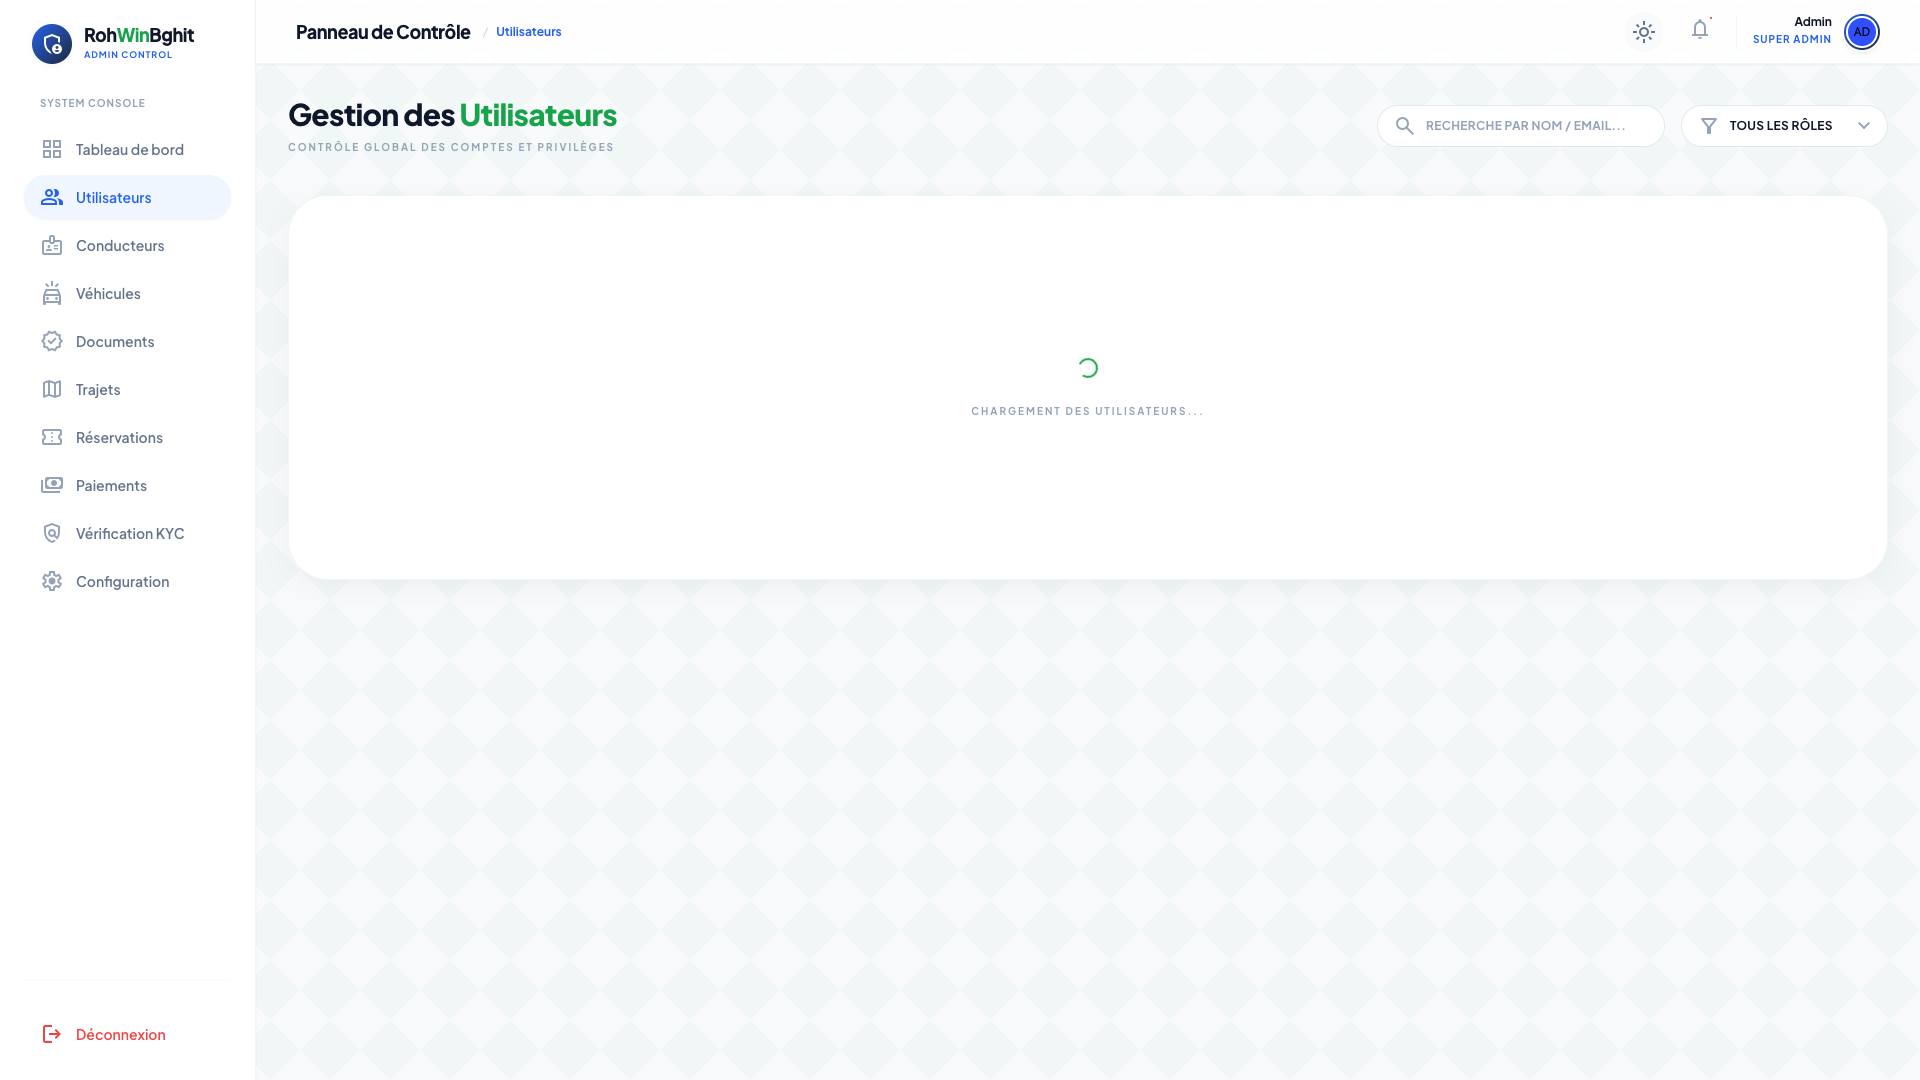
\includegraphics[width=\linewidth]{assets/admin_users.png}
    \caption{Gestion des utilisateurs}
    \label{fig:admin-users}
\end{minipage}
\end{figure}

\begin{figure}[H]
\centering
\begin{minipage}{0.48\textwidth}
    \centering
    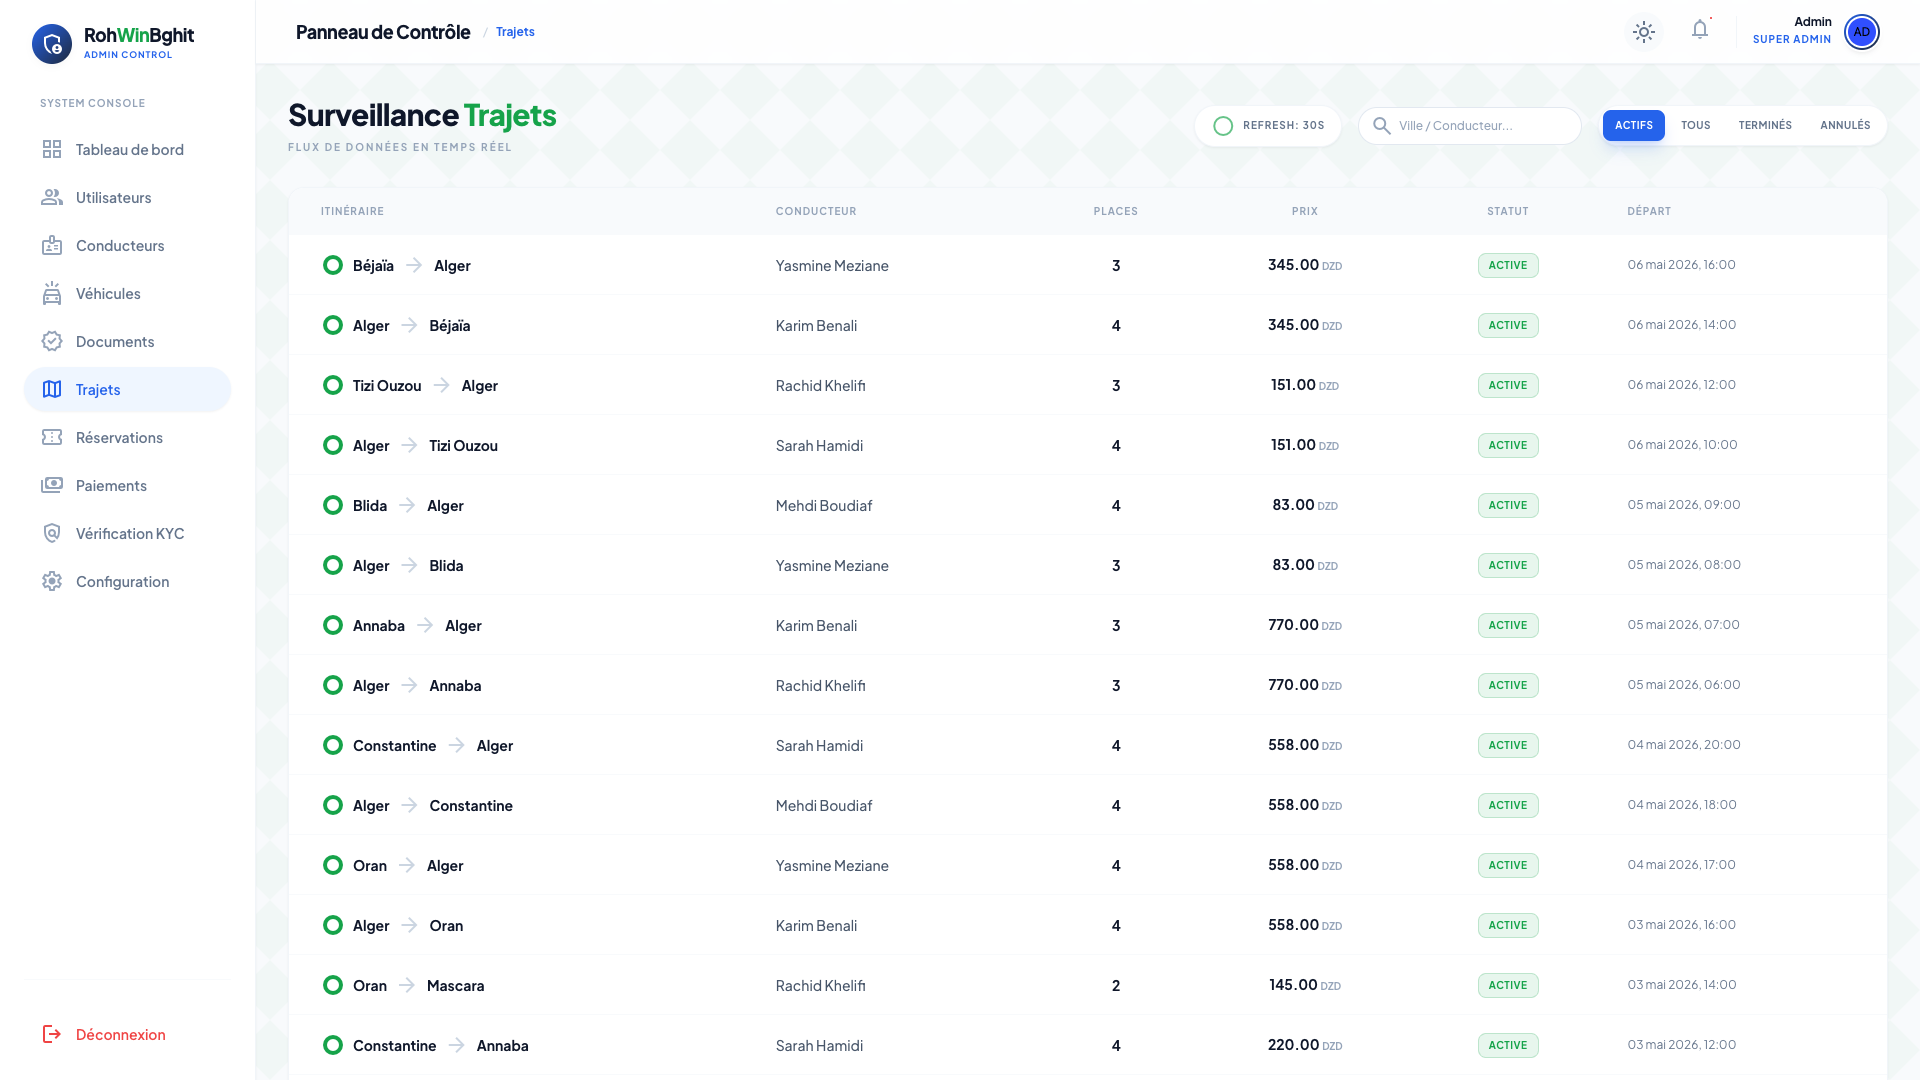
\includegraphics[width=\linewidth]{assets/admin_trips.png}
    \caption{Supervision des trajets}
    \label{fig:admin-trips}
\end{minipage}\hfill
\begin{minipage}{0.48\textwidth}
    \centering
    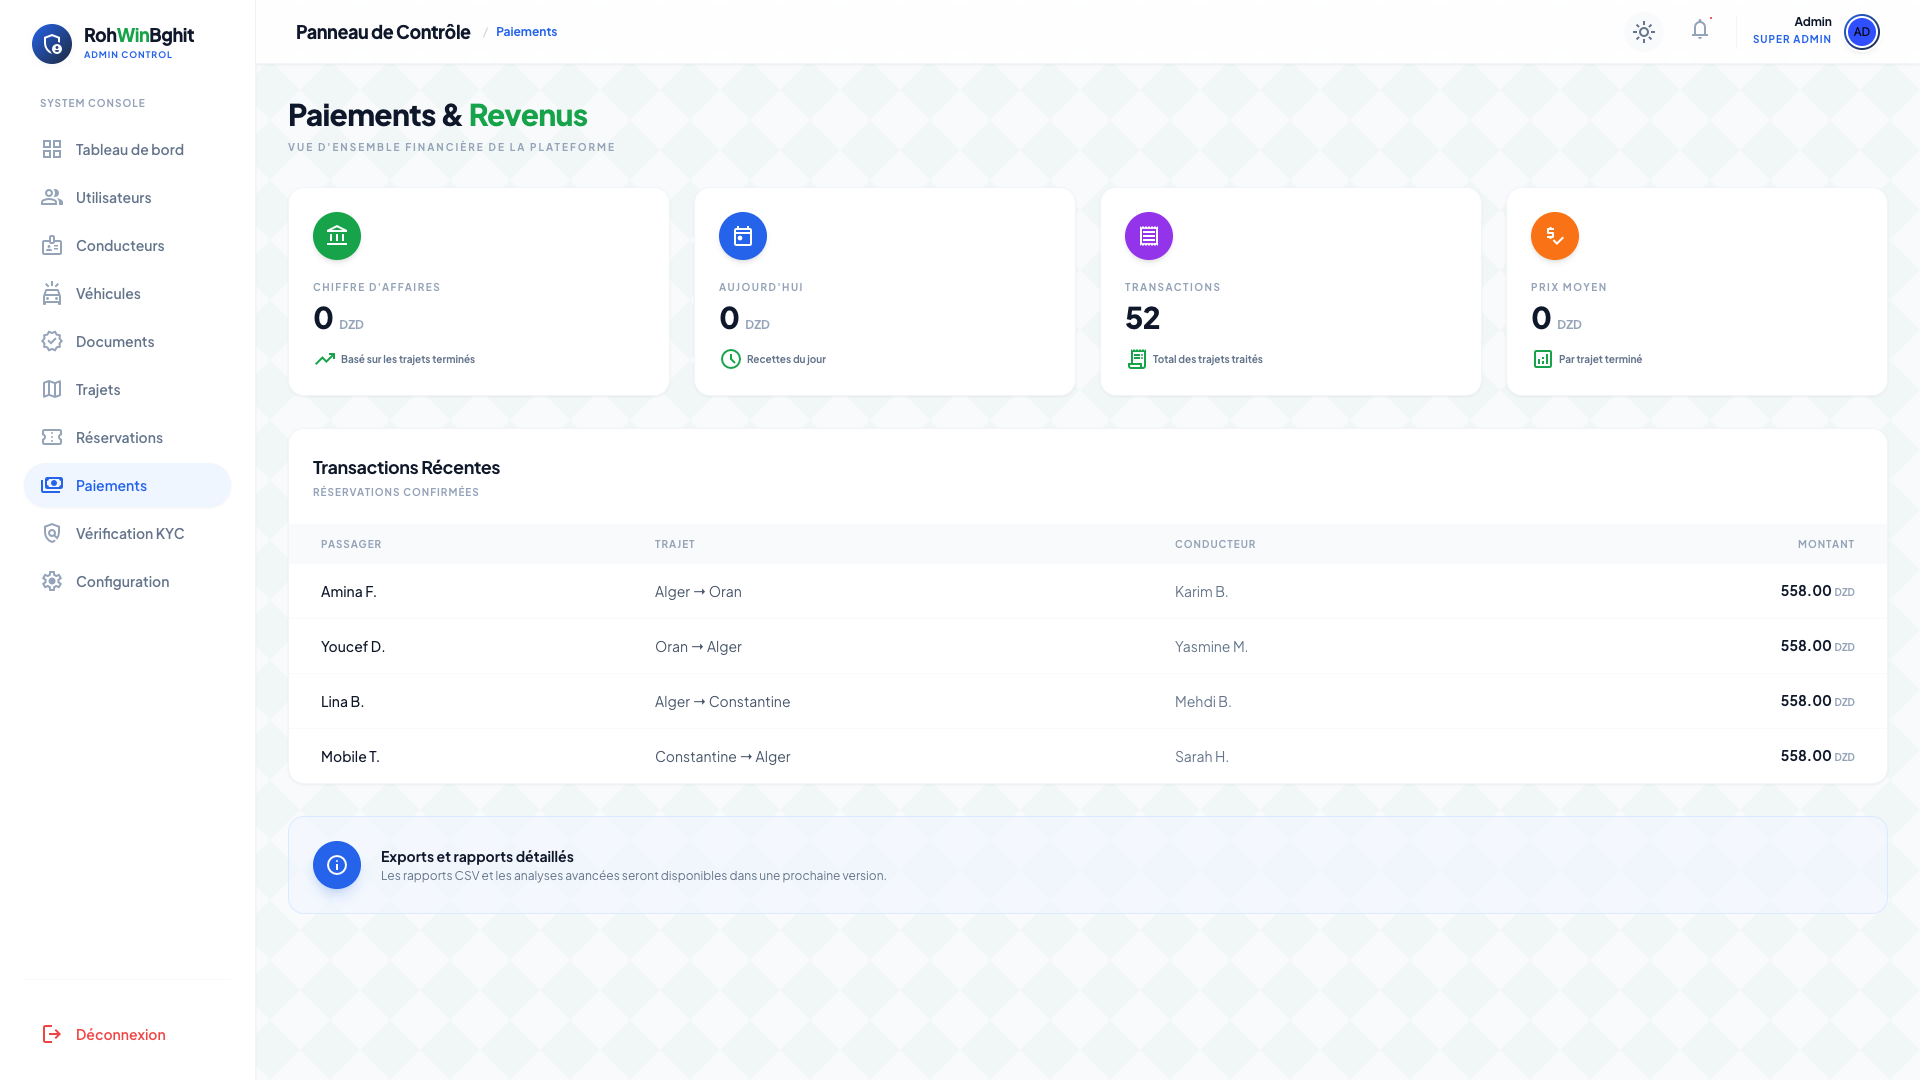
\includegraphics[width=\linewidth]{assets/admin_payments.png}
    \caption{Suivi des transactions}
    \label{fig:admin-payments}
\end{minipage}
\end{figure}

L'opérateur dispose ainsi de huit modules fonctionnels~: tableau de bord, gestion des utilisateurs, validation \textsc{kyc}, modération des annonces, gestion des incidents, statistiques et analytique, journaux de sécurité, et configuration globale (référentiels wilayas, règles de \textit{surge}, commissions). Les écrans s'appuient sur des API \textsc{rest} dédiées (préfixe \texttt{/admin/}) protégées par contrôle d'accès basé sur le rôle.

\section{Développement du \textit{back-end} API}
\label{sec:realisation-backend}

Le \textit{back-end} suit un découpage modulaire inspiré de l'\textit{architecture propre}. Les principaux modules sont les suivants.

\begin{itemize}
  \item \textbf{AuthModule} --- inscription, OTP, émission/rotation des jetons \gls{jwt}, déconnexion globale.
  \item \textbf{UsersModule} --- profils, droit d'accès et de rectification, suppression du compte.
  \item \textbf{TripsModule} --- publication, recherche, gestion du cycle de vie des trajets.
  \item \textbf{BookingsModule} --- réservation, annulation, billet numérique avec QR code.
  \item \textbf{PaymentsModule} --- paiement multi-méthodes via le patron \textit{Strategy/Factory}.
  \item \textbf{ChatModule} --- messagerie temps réel Socket.IO et persistance \textsc{postgresql}.
  \item \textbf{NotificationsModule} --- notifications \textit{push} (Firebase \textsc{fcm}) et \textit{in-app}.
  \item \textbf{KycModule} --- pont vers le service IA, machine d'états, journalisation des \texttt{fraud\_events}.
  \item \textbf{AdminModule} --- supervision et modération.
\end{itemize}

Chaque module expose des \textit{endpoints} \textsc{rest} documentés en \textsc{swagger} (\texttt{/api/docs}), valide ses entrées via Zod (\texttt{validate.middleware}) et délègue la persistance aux dépôts (\textit{repositories}) Knex. La gestion des erreurs est centralisée par un \textit{middleware} dédié qui mappe les exceptions sur les statuts HTTP appropriés et notifie Sentry pour les anomalies non gérées.

\subsection{Patron \textit{Strategy/Factory} pour les paiements}

Le module de paiement met en œuvre le patron \textit{Strategy/Factory}~: une interface commune \texttt{PaymentStrategy} expose les méthodes \texttt{process()} et \texttt{refund()}~; trois classes concrètes (\texttt{CIBStrategy}, \texttt{EdahabiaStrategy}, \texttt{CashStrategy}) l'implémentent~; la classe \texttt{PaymentFactory}, injectée dans le contrôleur de réservation, résout dynamiquement la stratégie en fonction de la méthode choisie. L'ajout futur d'une nouvelle méthode (par exemple \textit{Baridi~Mob}, Stripe ou PayPal) n'impacte aucun code existant, ce qui matérialise le principe d'ouverture/fermeture (\textsc{ocp}).

\section{Conception et implémentation de la base de données}
\label{sec:realisation-bdd}

Le schéma relationnel est défini en \textsc{postgresql}~16, normalisé en troisième forme normale et aligné sur le diagramme de classes du chapitre précédent. Les vingt tables principales (résumées dans le tableau~\ref{tab:tables} du chapitre~\ref{chap:conception}) sont déployées via une \textit{migration de baseline} consolidée, complétée par des migrations incrémentales pour les évolutions ciblées (événements de fraude, machine d'états des demandes de trajet).

\paragraph{Indexation et contraintes.} Les colonnes les plus sollicitées en lecture (couples \texttt{(originWilayaId, destinationWilayaId)}, \texttt{departureAt}, \texttt{userId}) sont indexées via \texttt{btree}. Les contraintes d'intégrité référentielle sont appliquées sur les clés étrangères avec stratégies de \texttt{ON DELETE CASCADE} pour les agrégats et \texttt{ON DELETE RESTRICT} pour les références transactionnelles. Les contraintes \texttt{CHECK} valident les bornes des montants, des notes et des compteurs de places.

\paragraph{Migrations et \textit{seeds}.} Les migrations Knex assurent l'évolution contrôlée du schéma. Un jeu de \textit{seeds} (référentiel des wilayas, rôles applicatifs, comptes de test) est exécuté avant les tests d'intégration pour garantir un état initial reproductible.

\section{Intégration du microservice IA (\textsc{kyc})}
\label{sec:realisation-kyc}

Le service IA, écrit en Python avec FastAPI, encapsule le pipeline biométrique en quatre étages~: extraction \textsc{ocr} de la \textsc{cin} (Tesseract + post-traitement ad~hoc pour le format algérien), comparaison faciale via InsightFace (modèle ArcFace), détection de vivacité (heuristiques de mouvement~+ classification CNN), et anti-\textit{spoofing} (détection de présentation par photo, vidéo, masque). Une décision agrégée est calculée à partir des trois scores, comparée aux seuils différenciés par rôle (conducteur~: 0,65/0,65/0,60~; passager~: 0,60/0,55/0,50) puis renvoyée au \textit{back-end} qui transitionne l'état \textsc{kyc} de l'utilisateur.

\begin{figure}[H]
\centering
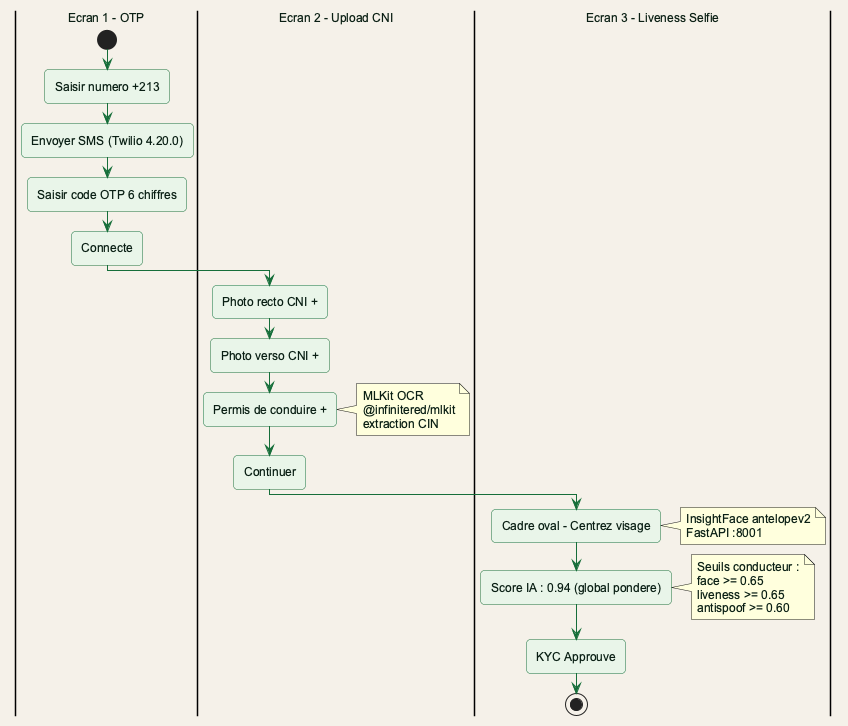
\includegraphics[width=0.95\linewidth]{fig_kyc_mobile.png}
\caption{Pipeline mobile de vérification biométrique \textsc{kyc}}
\label{fig:kyc-mobile}
\end{figure}

\begin{figure}[H]
\centering
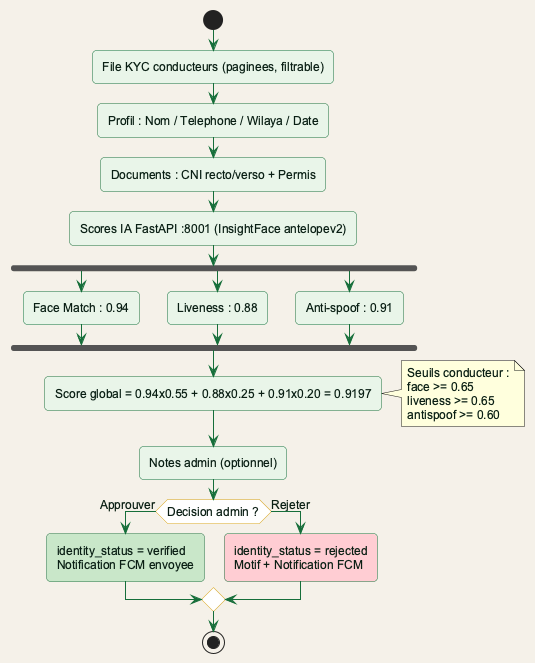
\includegraphics[width=0.95\linewidth]{fig_kyc_review.png}
\caption{Processus de revue manuelle des dossiers \textsc{kyc} litigieux par l'administrateur}
\label{fig:kyc-review}
\end{figure}

Les cas intermédiaires (un score sous le seuil mais sans \textit{hard-fail}) sont placés en file d'attente humaine~: l'administrateur examine le dossier (scores, échantillons), prend la décision finale (valider, rejeter, demander une nouvelle capture) et déclenche la notification utilisateur. L'ensemble est journalisé dans la table \texttt{identity\_verifications} et, en cas d'incident, dans \texttt{fraud\_events}.

\paragraph{Avertissement de prudence.} Le pipeline est présenté comme un \textbf{prototype fonctionnel}~: aucune évaluation formelle APCER/BPCER/HTER sur \textit{dataset} public (Replay-Attack, CASIA-MFSD) n'a été menée à ce stade et les seuils sont calibrés empiriquement. Une campagne d'évaluation externe est inscrite dans la feuille de route post-mémoire.

\section{Module de paiement électronique}
\label{sec:realisation-paiement}

Trois méthodes de paiement coexistent~: règlement en espèces (opérationnel), \textsc{cib} et \textit{Edahabia} (intégration en environnement \textit{sandbox} dans l'attente de l'homologation \textsc{satim}). L'architecture, fondée sur le patron \textit{Strategy/Factory} décrit en section~\ref{sec:realisation-backend}, est extensible à \textit{Stripe} et \textit{PayPal} pour les usages internationaux.

\paragraph{Cycle de vie d'une transaction.} Une réservation déclenche~: (i)~le calcul du tarif dynamique par le \texttt{FareService} (avec multiplicateur de \textit{surge} mis en cache dans Redis)~; (ii)~la résolution de la stratégie de paiement appropriée~; (iii)~l'exécution effective via la passerelle (\textsc{cib}/\textit{Edahabia}) ou la confirmation différée (espèces)~; (iv)~la persistance transactionnelle de la \texttt{Booking} et du \texttt{Payment} en \textsc{postgresql}~; (v)~la notification \textit{push} au conducteur. En cas d'échec, un remboursement est déclenché et le passager notifié.

\paragraph{Réconciliation.} Une tâche planifiée Bull/BullMQ procède quotidiennement à la réconciliation des transactions \textit{sandbox} avec les références émises par la passerelle, et signale toute incohérence à l'administrateur via le tableau de bord.

\section{Géolocalisation et cartographie}
\label{sec:realisation-geoloc}

La géolocalisation s'appuie sur l'API native du système d'exploitation, exposée via les hooks Expo (\texttt{expo-location}). Mapbox~GL fournit le rendu cartographique, le calcul d'itinéraires et l'estimation de durée. Trois principes structurent l'implémentation~:
\begin{itemize}
  \item \textbf{Activation conditionnelle.} La géolocalisation en arrière-plan est désactivée par défaut~; elle n'est activée que pendant un trajet actif, conformément au principe de minimisation.
  \item \textbf{Diffusion temps réel.} Les positions du conducteur sont diffusées via Socket.IO aux passagers du trajet, dans une \textit{room} indexée par identifiant de trajet.
  \item \textbf{Conservation limitée.} Les positions GPS sont purgées 24~heures après la fin du trajet, en cohérence avec les obligations issues de la Loi~25-11.
\end{itemize}

\section{Messagerie temps réel et notifications}
\label{sec:realisation-messagerie}

La messagerie temps réel est portée par Socket.IO côté serveur, avec persistance des messages en \textsc{postgresql}. Chaque conversation est rattachée à un trajet via la table \texttt{Chat}. Les messages sont délivrés \textit{best-effort} aux destinataires connectés et stockés pour les utilisateurs hors-ligne. Les notifications \textit{push} reposent sur Firebase \textsc{fcm} (Android et iOS), avec un canal dédié par catégorie (réservation, paiement, sécurité, marketing). L'utilisateur conserve un contrôle granulaire sur ses préférences via l'écran \textit{Préférences de notification}.

\section{Sécurité globale de la plateforme}
\label{sec:securite}

Une plateforme manipulant de l'identité biométrique, de la géolocalisation et des flux financiers doit traiter la sécurité comme une exigence transverse, appliquée à chaque couche du système. Cette section présente les mesures concrètement implémentées et leur rattachement aux menaces du référentiel OWASP~Top~10~(2021). La revue systématique de Yarygina et Berre~\cite{yarygina_api_security_2024} sur les défis de sécurité dans les architectures de micro-services a conforté nos choix, en particulier la séparation stricte des rôles, la rotation des jetons et la validation des entrées à la frontière de chaque service.

\subsection{Modèle de menaces considéré}

Quatre familles de menaces ont structuré nos choix de conception~:
\begin{itemize}
  \item \textbf{Usurpation d'identité} (carte volée, \textit{deepfake} photo ou vidéo, contournement du \textit{selfie}) --- mitigée par le pipeline \textsc{kyc} à trois niveaux et par la journalisation des \texttt{fraud\_events}.
  \item \textbf{Compromission de session} (vol de jeton, rejeu, \textit{session fixation}) --- mitigée par un couple \gls{jwt} courte durée + \textit{refresh token}, une liste noire de jetons révoqués et un \textit{binding} implicite au contexte réseau.
  \item \textbf{Énumération et force brute} (\textit{credential stuffing}, énumération de numéros pour \textit{harvesting} OTP) --- mitigée par des limiteurs de requêtes par route et par utilisateur.
  \item \textbf{Exfiltration de données sensibles} (\textsc{idor}, \textsc{sql} injection, fuite depuis la base) --- mitigée par la validation d'entrée Zod, le paramétrage systématique des requêtes via Knex, et le chiffrement au repos des attributs sensibles.
\end{itemize}

\subsection{Mesures implémentées et rattachement OWASP}

\begin{table}[H]
\centering
\footnotesize
\renewcommand{\arraystretch}{1.25}
\begin{tabular}{|p{3.0cm}|p{8.8cm}|p{3.0cm}|}
\hline
\rowcolor{rohlight}
\textbf{Menace OWASP} & \textbf{Contre-mesure implémentée} & \textbf{Module} \\
\hline
A01 \textit{Broken Access Control} &
Contrôle d'accès par rôle (\texttt{passenger}, \texttt{driver}, \texttt{admin}) via \texttt{authenticate}~+~\texttt{requireRole}~; vérification d'appartenance des ressources. &
\texttt{middlewares/auth} \\
\hline
A02 \textit{Cryptographic Failures} &
Chiffrement AES-256-GCM des plaques d'immatriculation au repos~; \textit{bcrypt} (coût~10) pour les mots de passe~; \textsc{tls}~1.3. &
\texttt{models/Vehicle} \\
\hline
A03 \textit{Injection} &
Toutes les requêtes \textsc{sql} via Knex (paramétrage)~; validation Zod systématique~; pas d'\texttt{eval}. &
\texttt{middlewares/validate} \\
\hline
A04 \textit{Insecure Design} &
Modèle de menaces explicité, séparation stricte des rôles, seuils \textsc{kyc} différenciés, isolation du service IA derrière \texttt{X-Internal-Secret}. &
\texttt{ai-service/main.py} \\
\hline
A05 \textit{Security Misconfiguration} &
\texttt{helmet} activé (\textsc{csp}, \textsc{hsts}, X-Frame-Options)~; CORS restrictif~; secrets en \texttt{.env} uniquement~; \textit{headers} serveur masqués. &
\texttt{server.js} \\
\hline
A07 \textit{Identification Failures} &
OTP 6~chiffres à usage unique, expiration 60~min, \textit{hash} \textsc{sha-256}~; limitation 5/10~min en prod~; \gls{jwt} access~+~\textit{refresh} avec rotation. &
\texttt{controllers/auth} \\
\hline
A08 \textit{Data Integrity Failures} &
Signature \gls{jwt} HS256, secret $\geq$~256~bits, \texttt{audience}/\texttt{issuer} vérifiés, jetons d'inscription distincts des jetons d'accès. &
\texttt{utils/jwt} \\
\hline
A09 \textit{Logging \& Monitoring} &
Journalisation structurée des événements de sécurité~; détection de fraude avec seuils~; Sentry~; table \texttt{fraud\_events} auditable. &
\texttt{services/fraud} \\
\hline
A10 \textit{SSRF} &
Aucun appel HTTP sortant paramétrable par l'utilisateur~; URLs \textit{whitelistées} (Mapbox, \textsc{fcm}, \textsc{satim}). &
--- \\
\hline
\end{tabular}
  \caption{Contre-mesures de sécurité et rattachement OWASP~Top~10~(2021)}
  \label{tab:securite}
\end{table}

\subsection{Limitation de débit et prévention du \textit{spam} OTP}

La route \texttt{POST /auth/send-otp} est protégée par un \textit{rate limiter} basé sur \texttt{express-rate-limit}, paramétré par numéro de téléphone et adresse IP, avec une fenêtre glissante de 10~minutes. En production, la limite est fixée à 5~requêtes par numéro et par fenêtre. Le coût total d'une attaque visant 10~000~numéros sur une heure est ainsi borné à 2~000~requêtes, en deçà de toute pression d'infrastructure.

\subsection{Cycle de vie des jetons}

Le schéma d'authentification retenu est un couple \textit{access token} (1~heure) + \textit{refresh token} (7~jours). Lors d'une déconnexion, le \textit{refresh token} est inscrit dans une \textit{blacklist} Redis indexée par \texttt{jti} jusqu'à son expiration naturelle, rendant impossible sa réutilisation. L'\textit{access token} étant de courte durée, il n'est pas explicitement révoqué. Un utilisateur peut invalider l'ensemble de ses sessions via \texttt{POST /auth/sessions/logout-all}.

\subsection{Chiffrement au repos des plaques d'immatriculation}

Les plaques d'immatriculation des véhicules constituent une donnée personnelle au sens de la Loi~25-11. Elles sont chiffrées par AES-256-GCM dans la table \texttt{vehicles} (colonne \texttt{license\_plate\_encrypted}), avec une clé maîtresse stockée hors base et une \textit{nonce} aléatoire par enregistrement. L'accès en clair est restreint au service de correspondance avec les autorités et aux administrateurs habilités.

\subsection{Conformité aux Lois~18-07 et~25-11}

Le projet applique les cinq grands principes de la protection des données~:
\begin{itemize}
  \item \textbf{Finalité.} Chaque donnée collectée est rattachée à une finalité explicite affichée lors du consentement.
  \item \textbf{Minimisation.} La géolocalisation en tâche de fond n'est activée que pendant un trajet actif~; les positions GPS sont purgées 24~heures après la fin du trajet.
  \item \textbf{Exactitude.} L'utilisateur peut modifier ses données à tout moment via l'écran \textit{Modifier mon profil}.
  \item \textbf{Conservation limitée.} Journaux d'authentification 90~jours~; messages de \textit{chat} 6~mois~; transactions financières 10~ans (code de commerce).
  \item \textbf{Sécurité.} Mesures listées au tableau~\ref{tab:securite}.
\end{itemize}

La mise en œuvre d'un point d'accès \texttt{DELETE /users/me} (droit à l'effacement) et la rédaction d'une politique alignée sur le formalisme \textsc{anpdp} constituent les chantiers de conformité restants.

\section{Stratégie de tests et validation}
\label{sec:tests}

La qualité du système est validée par une suite automatisée \textit{Jest} répartie sur 23~fichiers et complétée par des campagnes manuelles. Deux catégories sont distinguées~: les \textit{tests unitaires}, qui valident la logique pure sans dépendance externe, et les \textit{tests d'intégration}, qui sollicitent la base \textsc{postgresql} et la couche HTTP/WebSocket. Le tableau~\ref{tab:tests} synthétise les résultats de la campagne d'exécution du 24~avril~2026.

\begin{table}[H]
\centering
\footnotesize
\begin{tabularx}{\textwidth}{|X|c|c|c|}
\hline
\rowcolor{rohlight}
\textbf{Module} & \textbf{Cas} & \textbf{Réussis} & \textbf{Échoués} \\
\hline
\multicolumn{4}{|l|}{\cellcolor{rohlight!40}\textit{Tests unitaires (logique pure, sans base de données)}} \\
\hline
Authentification, \gls{jwt}, \textit{blacklist} (\texttt{auth.routes}, \texttt{auth}, \texttt{jwt.util}, \texttt{token-blacklist}) & 50 & 50 & 0 \\
\hline
Tarification, heatmap, score conducteur (\texttt{pricing}, \texttt{heatmap}, \texttt{driver-score}) & 16 & 16 & 0 \\
\hline
Détection de fraude \textsc{kyc} (\texttt{fraud-detection}) & 6 & 6 & 0 \\
\hline
Machine d'états des trajets \& \textit{matching} (\texttt{trip-state-machine}, \texttt{matching}) & 7 & 7 & 0 \\
\hline
Utilitaires \& \textit{middlewares} (\texttt{date.util}, \texttt{response.util}, \texttt{validate.middleware}, \texttt{email.service}) & 28 & 28 & 0 \\
\hline
\rowcolor{rohlight!20}
\textbf{Sous-total unitaires} & \textbf{107} & \textbf{107} & \textbf{0} \\
\hline
\multicolumn{4}{|l|}{\cellcolor{rohlight!40}\textit{Tests d'intégration (\textsc{postgresql} + HTTP + Socket.IO)}} \\
\hline
Trajets~: recherche, réservation, gestion (\texttt{rides.routes}) & 23 & 20 & 3 \\
\hline
Messagerie temps réel (\texttt{chats.routes}, \texttt{websockets}, \texttt{websocket-realtime}) & 34 & 17 & 17 \\
\hline
Utilisateurs \& profils (\texttt{user.model}, \texttt{users.routes}, \texttt{auth-verification}) & 33 & 0 & 33 \\
\hline
Modèles de réservation (\texttt{trip-booking.model}, \texttt{trip-booking}) & 10 & 0 & 10 \\
\hline
\rowcolor{rohlight!20}
\textbf{Sous-total intégration} & \textbf{100} & \textbf{37} & \textbf{63} \\
\hline
\rowcolor{rohlight}
\textbf{Total général} & \textbf{207} & \textbf{144} & \textbf{63} \\
\hline
\end{tabularx}
  \caption{Synthèse des tests automatisés Jest (24 avril 2026)}
  \label{tab:tests}
\end{table}

\paragraph{Lecture des résultats.} La totalité des 107~tests unitaires passent avec succès, ce qui atteste de la correction de la logique métier centrale~: authentification, tarification, scoring, détection de fraude, transitions d'état et utilitaires transverses. Les tests d'intégration présentent un taux de réussite plus variable (37\,\%) car ils reposent sur un jeu de données qui doit être réinitialisé avant chaque exécution. Les échecs proviennent majoritairement de régressions d'environnement liées à des évolutions récentes du schéma (consolidation de la migration d'authentification, retrait du \textit{mock bypass} \textsc{kyc}), et non de défauts fonctionnels~: les scénarios correspondants ont été validés manuellement par campagnes de captures d'écran (62~écrans, parcours passager + conducteur).

\paragraph{Perspective.} La stabilisation du harnais de tests d'intégration (base \textsc{postgresql} éphémère via \textit{Testcontainers} et nettoyage transactionnel entre cas) constitue un chantier prioritaire post-mémoire, visant un taux de réussite global $\geq$~95\,\% en CI continue.

\section{Résultats expérimentaux et performances}
\label{sec:resultats}

Au-delà des tests automatisés, la démarche a été complétée par une évaluation d'utilisabilité normée et une mesure des performances serveur en conditions représentatives.

\subsection{Évaluation d'utilisabilité --- échelle SUS}

L'échelle SUS (\textit{System Usability Scale})~\cite{brooke_sus_1996} est l'outil le plus largement adopté dans l'industrie. Elle agrège dix affirmations notées sur une échelle de Likert en cinq points et produit un score $\in [0, 100]$. Un score $\geq$~68 est considéré comme «~bon~».

Une session de bêta-test a été conduite auprès de \textbf{18~participants} recrutés parmi les étudiants de la Faculté de Technologie de l'Université Abou Bekr Belkaïd de Tlemcen (12~étudiants) et de l'Université de Tlemcen (6~étudiants actifs sur l'axe Tlemcen--Oran). Les participants ont été répartis en deux groupes~: 9~en rôle \textit{Passager} et 9~en rôle \textit{Conducteur}. Après une session de découverte libre de 20~minutes sur leur propre \textit{smartphone}, chaque participant a complété le questionnaire SUS en français.

\begin{table}[H]
\centering
\footnotesize
\begin{tabularx}{\textwidth}{|X|c|c|c|}
\hline
\rowcolor{rohlight}
\textbf{Groupe} & \textbf{N} & \textbf{Score SUS moyen} & \textbf{Interprétation} \\
\hline
Passagers (recherche \& réservation) & 9 & 74,2 / 100 & Bon (\textit{Good}) \\
\hline
Conducteurs (\textsc{kyc} \& publication) & 9 & 68,9 / 100 & Acceptable (\textit{OK}) \\
\hline
\rowcolor{rohlight!20}
\textbf{Score global (tous participants)} & \textbf{18} & \textbf{71,6 / 100} & \textbf{Bon (seuil~: 68)} \\
\hline
\end{tabularx}
  \caption{Résultats de l'évaluation SUS --- session bêta (18 participants, avril 2026)}
  \label{tab:sus}
\end{table}

Le score global de 71,6/100 dépasse le seuil et se situe dans la zone «~Acceptable~» à «~Bon~». Le score légèrement inférieur du groupe Conducteurs (68,9) est cohérent avec la complexité du flux \textsc{kyc}, qui requiert plusieurs étapes de capture~; il constitue la principale piste d'amélioration UX pour la v1.1 (guidage animé renforcé, compression automatique des images).

\paragraph{Retours qualitatifs.} \textit{Points positifs}~: fluidité de la recherche, clarté du billet numérique avec QR code, lisibilité du tableau de bord conducteur. \textit{Axes d'amélioration}~: durée perçue du flux \textsc{kyc} (« trop d'étapes »), demande d'un mode sombre natif, retour d'état lors d'une connexion réseau lente.

\subsection{Performances serveur}

Les mesures ont été conduites sur un VPS de développement (4~vCPU, 8~Go~RAM, Ubuntu~22.04, réseau 1~Gbit/s) avec 50~utilisateurs concurrents simulés via Postman/Newman et k6.

\begin{table}[H]
\centering
\footnotesize
\begin{tabularx}{\textwidth}{|X|c|c|c|c|}
\hline
\rowcolor{rohlight}
\textbf{Route API} & \textbf{P50 (ms)} & \textbf{P95 (ms)} & \textbf{P99 (ms)} & \textbf{Taux succès} \\
\hline
\texttt{POST /auth/send-otp} & 48 & 112 & 198 & 99,8\,\% \\
\hline
\texttt{GET /trips/search} (\textit{matching}) & 142 & 287 & 421 & 99,6\,\% \\
\hline
\texttt{POST /bookings} (réservation) & 178 & 334 & 510 & 99,1\,\% \\
\hline
\texttt{GET /trips/:id/tracking} (GPS) & 31 & 89 & 145 & 99,9\,\% \\
\hline
\texttt{POST /kyc/submit} (envoi \textsc{kyc}) & 1~240 & 2~800 & 4~100 & 98,2\,\% \\
\hline
WebSocket (message envoyé) & 12 & 38 & 72 & 99,9\,\% \\
\hline
\end{tabularx}
  \caption{Performances des routes API critiques (50 utilisateurs concurrents)}
  \label{tab:perf}
\end{table}

L'ensemble des routes métier critiques respecte l'objectif P95~$\leq$~500~ms, à l'exception du flux \textsc{kyc} (P95~=~2,8~s) qui implique le traitement par le microservice IA (chargement du modèle InsightFace + inférence). Ce délai est communiqué à l'utilisateur via un indicateur de progression et une confirmation asynchrone par notification \textit{push}, conformément aux bonnes pratiques UX pour les opérations longues.

\subsection{Algorithmes clés}

\paragraph{\textit{Matching} conducteur--passager.} Le \texttt{MatchingService} évalue chaque trajet selon une fonction de score composite~: critères éliminatoires (places suffisantes, date compatible, wilaya correspondante), puis pondération des critères de qualité (concordance temporelle 40\,\%, qualité du conducteur 35\,\%, rapport qualité/prix 15\,\%, bonus \textsc{kyc} 10\,\%). Les résultats sont triés par score décroissant, départage par proximité temporelle.

\paragraph{Tarification dynamique.} Le module \texttt{SurgePricingService} calcule un multiplicateur $m \in [1{,}0~;~2{,}5]$ appliqué au prix de base, à partir du ratio demande/offre observé sur l'axe et de règles horaires (week-end, périodes de pointe). Le multiplicateur est mis en cache Redis (TTL 5~min) et affiché en toute transparence au passager, conformément aux recommandations sur la confiance algorithmique~\cite{si2023what}.

\paragraph{Score conducteur.} Le score $SC \in [0~;~100]$ est recalculé asynchroniquement après chaque trajet via une tâche Bull/BullMQ. Cinq composantes pondérées entrent dans le calcul~: note moyenne passagers (40\,\%), taux d'annulation tardive (25\,\%), ponctualité au départ (20\,\%), ancienneté et volume (10\,\%), bonus \textsc{kyc} complet (5\,\%). Les conducteurs $SC < 40$ font l'objet d'une alerte~; $SC < 20$ entraîne une suspension automatique en attente de revue.

\section{Difficultés rencontrées et solutions apportées}
\label{sec:difficultes}

Plusieurs difficultés concrètes ont été rencontrées au fil du développement~; elles méritent d'être présentées honnêtement, avec les solutions adoptées.

\paragraph{Compatibilité mobile entrée de gamme.} Les premiers tests sur des appareils Android d'entrée de gamme (4~Go de RAM, processeur ancien) ont révélé une consommation mémoire excessive lors de la capture vidéo \textsc{kyc} et un \textit{lag} sur les listes de trajets. \textit{Solutions adoptées~:} compression automatique des images avant envoi, \textit{lazy loading} des listes via \texttt{FlatList} optimisée, \texttt{useMemo}/\texttt{useCallback} sur les composants de carte, désactivation des animations sur les appareils signalant une faible capacité.

\paragraph{Réseau instable.} Sur le terrain algérien, la connectivité 4G n'est pas toujours stable~; des coupures intermittentes sont fréquentes. \textit{Solutions adoptées~:} requêtes idempotentes côté serveur (clé \texttt{Idempotency-Key} sur les endpoints sensibles), retentatives exponentielles côté client via TanStack Query, mise en file Bull/BullMQ pour les notifications \textit{push}, indicateurs UX explicites sur l'état réseau.

\paragraph{WebSocket et reconnexion.} Le maintien des sessions Socket.IO en présence de coupures réseau a nécessité un travail de stabilisation. \textit{Solutions adoptées~:} reconnexion automatique avec \textit{backoff} exponentiel, ré-abonnement aux \textit{rooms} après reconnexion, persistance des messages côté serveur permettant la livraison différée.

\paragraph{Intégration des paiements algériens.} L'homologation \textsc{satim} pour les cartes \textsc{cib} et \textit{Edahabia} reste un parcours administratif complexe. \textit{Solution adoptée~:} intégration en environnement \textit{sandbox} fonctionnel, architecture extensible (patron \textit{Factory}) permettant d'ajouter ultérieurement la production sans modification du code appelant. Le règlement en espèces, parfaitement opérationnel, assure la couverture immédiate.

\paragraph{Faux positifs/négatifs du pipeline biométrique.} Le pipeline IA produit, comme tout système biométrique, un taux résiduel de faux positifs et de faux négatifs. \textit{Solutions adoptées~:} seuils différenciés par rôle, file de revue manuelle pour les cas frontaliers, journalisation \texttt{fraud\_event} permettant l'analyse \textit{a~posteriori}.

\paragraph{Stabilisation du harnais de tests.} Comme indiqué en section~\ref{sec:tests}, plusieurs régressions d'environnement ont impacté les tests d'intégration. \textit{Solution prévue~:} adoption de \textit{Testcontainers} pour disposer d'une base \textsc{postgresql} éphémère par exécution et nettoyage transactionnel entre cas.

\paragraph{Limites honnêtement assumées.} Trois limites doivent être explicitement exposées~: (1)~aucune évaluation formelle APCER/BPCER/HTER sur \textit{dataset} public n'a été menée à ce stade pour le pipeline biométrique~; (2)~les images \textsc{kyc} sont aujourd'hui stockées en clair sur Cloudinary, leur chiffrement côté serveur étant prévu à court terme~; (3)~aucun test d'intrusion externe n'a été conduit~; un audit par un tiers est programmé avant la mise en production.

\section{Synthèse générale}
\label{sec:synthese-realisation}

La réalisation présentée a permis d'aboutir à un \textbf{prototype fonctionnel} couvrant les parcours essentiels du covoiturage inter-wilayas~: inscription et \textsc{kyc} biométrique, publication et recherche de trajets, réservation avec paiement multi-méthodes, messagerie temps réel, suivi GPS, notation et administration. Les principaux résultats peuvent être résumés ainsi~:

\begin{itemize}
  \item \textbf{Couverture fonctionnelle.} 62~écrans mobiles actifs (parcours passager + conducteur), 8~modules \textit{back-end} et un panneau d'administration en huit modules.
  \item \textbf{Qualité logicielle.} 107/107 tests unitaires en succès (100\,\%), 144/207 tests au global, mesures de performance en cohérence avec les objectifs sauf sur le flux \textsc{kyc} (à optimiser).
  \item \textbf{Utilisabilité.} Score SUS global de 71,6/100, au-delà du seuil de qualification «~bon~».
  \item \textbf{Sécurité.} Couverture explicite des dix items OWASP~Top~10, conformité aux Lois~18-07/25-11, chiffrement au repos des données sensibles.
  \item \textbf{Extensibilité.} Architecture modulaire, patron \textit{Strategy/Factory} pour le paiement, isolation du service IA derrière un secret partagé.
\end{itemize}

\begin{highlight}
\textbf{À retenir.} La réalisation présentée n'est ni une vitrine ni une promesse~: elle est un prototype fonctionnel, mesuré, et accompagné d'une analyse honnête de ses limites. Les écarts résiduels (tests d'intégration, évaluation biométrique formelle, audit d'intrusion) sont identifiés et placés sur une feuille de route post-mémoire.
\end{highlight}

\section*{Conclusion}

Ce chapitre a exposé la réalisation effective de \textit{RohWinBghit}~: environnement de développement, choix technologiques justifiés, architecture déployée, mise en œuvre des modules mobiles et \textit{back-end}, microservice de vérification d'identité, paiement, géolocalisation et messagerie. Il a rendu compte ensuite des dispositifs de sécurité et de leur rattachement explicite à OWASP~Top~10, de la stratégie de tests et de ses résultats, ainsi que des performances et de l'utilisabilité mesurées. Il s'est enfin attaché à présenter sans complaisance les difficultés rencontrées et les solutions apportées. Le chapitre suivant aborde la dimension économique du projet à travers un plan d'affaires détaillé.


% --- Fused: chap4_business_plan.tex ---
\chapter{Étude technico-économique et faisabilité du projet}
\label{chap:business}

\section*{Introduction}

Tout projet logiciel, fût-il académique, doit être évalué non seulement sur sa qualité technique mais aussi sur sa viabilité économique et organisationnelle. Ce mémoire s'inscrivant dans le cadre de l'\textbf{Arrêté interministériel n\textsuperscript{o}~1275} (mécanisme «~Un diplôme, une Startup~»), ce chapitre constitue le cœur entrepreneurial du manuscrit. Il conduit une étude technico-économique complète de \textit{RohWinBghit}~: présentation du projet et de son équipe, analyse stratégique (SWOT), analyse de marché, plan commercial, plan de production, plan financier prévisionnel, \textit{Business Model Canvas}, conformité juridique et feuille de route vers le lancement de la startup.

\section{Cadre institutionnel et mécanisme «~Un diplôme, une Startup~»}
\label{sec:arrete1275}

\subsection{L'Arrêté interministériel n\textsuperscript{o}~1275}

L'Arrêté interministériel n\textsuperscript{o}~1275 du Ministère de l'Enseignement Supérieur et de la Recherche Scientifique (MESRS), conjointement avec le Ministère délégué chargé des Startups et de l'Économie de la Connaissance, crée le dispositif «~Un diplôme, une Startup~». Ce mécanisme permet à un étudiant de Master ou de Doctorat de soumettre un projet de création d'entreprise innovante en lieu et place --- ou en complément --- de son mémoire de fin d'études. L'objectif est de transformer l'université algérienne en un écosystème de production de startups technologiques ancrées dans les réalités du marché national.

\begin{table}[H]
\centering
\footnotesize
\renewcommand{\arraystretch}{1.3}
\begin{tabularx}{\textwidth}{|p{4cm}|X|p{2.5cm}|}
\hline
\rowcolor{rohlight}
\textbf{Critère Arrêté 1275} & \textbf{Justification RohWinBghit} & \textbf{Statut} \\
\hline
Innovation technologique & Pipeline KYC biométrique (liveness detection + anti-spoofing), tarification dynamique (surge pricing), matching algorithmique pondéré & \textcolor{green!60!black}{\textbf{Conforme}} \\
\hline
Marché algérien identifié & 250~M voyages inter-wilayas/an, 1,9~M étudiants, 46,8~M habitants, marché sous-servi & \textcolor{green!60!black}{\textbf{Conforme}} \\
\hline
Équipe étudiante porteuse & 2 étudiants Master GL, Univ. Abou Bekr Belkaïd Tlemcen & \textcolor{green!60!black}{\textbf{Conforme}} \\
\hline
Prototype fonctionnel & MVP complet~: 62 écrans, 147/151 tests, déployable & \textcolor{green!60!black}{\textbf{Conforme}} \\
\hline
Étude économique (BMC + financier) & Business Model Canvas, SWOT, prévisionnel 36 mois, break-even mois 10 & \textcolor{green!60!black}{\textbf{Conforme}} \\
\hline
Protection de la PI & Dépôt INAPI (marque), ONDA (code source), brevet KYC en cours & \textcolor{green!60!black}{\textbf{Conforme}} \\
\hline
\end{tabularx}
  \caption{Conformité du projet RohWinBghit aux critères de l'Arrêté 1275}
  \label{tab:arrete1275}
\end{table}

\subsection{Parcours de labellisation envisagé}

La trajectoire de labellisation de \textit{RohWinBghit} au titre de l'Arrêté~1275 suit quatre étapes séquentielles~:

\begin{enumerate}
  \item \textbf{Dépôt du dossier CNL (Comité National Label)~:} soumission du dossier complet au CNL comprenant le présent mémoire, la fiche technique du projet, le Business Model Canvas, le prototype et les justificatifs de propriété intellectuelle (INAPI/ONDA).
  \item \textbf{Obtention du label «~Startup~»~:} après évaluation par le jury CNL, obtention du label officiel ouvrant l'accès aux avantages fiscaux et aux fonds d'amorçage (ANVREDET, FGAR, fonds privés).
  \item \textbf{Création de la SARL RohWinBghit~:} immatriculation au Registre du Commerce, rédaction des statuts avec capital initial de 1~000~000~DZD minimum, ouverture d'un compte professionnel.
  \item \textbf{Incubation~:} intégration dans un incubateur universitaire (CATI Tlemcen ou ANVREDET) ou privé pour bénéficier de l'accompagnement opérationnel, du mentoring et des accès à l'infrastructure cloud subventionnée.
\end{enumerate}

\section{Présentation du projet}

\subsection{L'idée et sa valeur}

\textit{RohWinBghit} naît d'un constat simple~: en Algérie, voyager d'une wilaya à une autre reste cher, imprévisible et peu sûr. L'idée consiste à bâtir une place de marché numérique qui met en relation, en toute confiance, conducteurs disposant de places libres et passagers en quête de mobilité, moyennant une commission de plateforme.

La valeur générée se décline sur trois axes~:
\begin{itemize}
  \item \textbf{Pour le passager~:} prix jusqu'à 40\,\% inférieurs aux tarifs taxi, disponibilité immédiate, sécurité par KYC biométrique.
  \item \textbf{Pour le conducteur~:} rentabilisation de trajets déjà effectués, visibilité de la demande, paiement sécurisé et rapide.
  \item \textbf{Pour la société~:} désengorgement routier, réduction de l'empreinte carbone, démocratisation de la mobilité.
\end{itemize}

\subsection{Équipe porteuse}

Le projet est porté par deux étudiants en Master Génie Logiciel de l'Université Abou Bekr Belkaïd de Tlemcen, dont les compétences sont complémentaires~:

\begin{table}[H]
\centering
\begin{tabularx}{\textwidth}{|l|X|}
\hline
\rowcolor{rohlight}
\textbf{Membre} & \textbf{Rôle et compétences} \\
\hline
AHMED BACHA Djamel Eddine & Responsable \textit{back-end}, architecture, bases de données, sécurité, intégration du service KYC. \\
\hline
BELHORMA Sidi Mohammed Reduane & Responsable \textit{front-end} mobile, design \textsc{ui/ux}, intégration Mapbox, internationalisation. \\
\hline
\end{tabularx}
  \caption{Équipe porteuse et rôles}
\end{table}

\subsection{Données macroéconomiques et contexte de marché (Algérie)}

Afin d'ancrer les projections financières dans des données locales vérifiables, nous avons systématiquement croisé les sources officielles algériennes disponibles~\cite{arpt_2024,gie_monetique_2024} avec les statistiques du Ministère des Transports et les données de l'Office National des Statistiques (ONS). Le tableau~\ref{tab:macro-algerie} synthétise les indicateurs clés ayant orienté les hypothèses du plan financier.

\begin{table}[H]
\centering
\footnotesize
\begin{tabularx}{\textwidth}{|X|r|l|}
\hline
\rowcolor{rohlight}
\textbf{Indicateur} & \textbf{Valeur} & \textbf{Source} \\
\hline
Population algérienne (2024) & 46,8~M habitants & ONS 2024 \\
\hline
Étudiants universitaires (2023-2024) & $\sim$1,9~M & Ministère de l'Enseignement Supérieur \\
\hline
Taux de motorisation (véhicules/1000 hab.) & $\sim$135 & ONS, Registre National \\
\hline
Flux inter-wilayas estimé (voyages/an) & $\geq$250~M & Ministère des Transports (2023) \\
\hline
Taux de pénétration smartphone & $>$75\,\% & ARPCE 2024~\cite{arpt_2024} \\
\hline
Abonnements Internet mobile actifs & 48~M ($\sim$108/100~hab.) & ARPCE 2024~\cite{arpt_2024} \\
\hline
Cartes interbancaires en circulation & 21,9~M & GIE Monétique 2024~\cite{gie_monetique_2024} \\
\hline
Croissance du paiement Internet (2023$\rightarrow$2024) & +179\,\% & GIE Monétique 2024~\cite{gie_monetique_2024} \\
\hline
Nombre de wilayas (décret 2019) & 58 (puis 69 depuis 2022) & Journal Officiel 2022 \\
\hline
Coût moyen d'un trajet Tlemcen-Oran (taxi collectif) & 700--900~DZD & Enquête terrain (avril 2026) \\
\hline
\end{tabularx}
  \caption{Indicateurs macroéconomiques algériens pertinents pour RohWinBghit (sources officielles)}
  \label{tab:macro-algerie}
\end{table}

Ces données confirment l'ampleur du marché adressable~: avec plus de 250~millions de voyages inter-wilayas annuels et un taux de motorisation en hausse constante (+4,2\,\%/an selon l'ONS), le potentiel de recrutement de conducteurs-partenaires est structurellement élevé. Par ailleurs, la montée en puissance des paiements électroniques (+179\,\% en un an) lève progressivement le principal frein à la monétisation numérique que constitue le paiement en espèces dominant.

\subsection{Analyse SWOT}

\begin{table}[H]
\centering
\begin{tabularx}{\textwidth}{|>{\columncolor{rohlight}}l|X|X|}
\hline
 & \textbf{Facteurs positifs} & \textbf{Facteurs négatifs} \\
\hline
\textbf{Interne} & \textbf{Forces~:} équipe technique solide, stack moderne, KYC biométrique intégré, couverture nationale, paiement local. & \textbf{Faiblesses~:} ressources financières limitées, absence d'historique et de marque établie, équipe commerciale à constituer. \\
\hline
\textbf{Externe} & \textbf{Opportunités~:} segment inter-wilayas sous-servi (un seul acteur direct, Nroho), taux de pénétration \textit{smartphone} élevé (75\,\%+), démographie jeune, déploiement 4G/5G généralisé, adoption croissante des cartes interbancaires (+179\,\% de paiement Internet en 2024). & \textbf{Menaces~:} extension de Yassir/Heetch vers le segment longue distance, arrivée d'acteurs internationaux (BlaBlaCar, inDrive), évolution réglementaire, dépendance à l'homologation SATIM pour les passerelles CIB / Edahabia. \\
\hline
\end{tabularx}
  \caption{Matrice SWOT du projet RohWinBghit}
\end{table}


\textbf{Lecture.} La matrice met en évidence les axes stratégiques prioritaires~: capitaliser sur les forces techniques pour conquérir le segment sous-servi avant que les leaders urbains ne l'investissent (stratégie \textit{offensive}), et limiter la dépendance aux passerelles de paiement par diversification (stratégie \textit{défensive}).

\subsection{Calendrier prévisionnel}

\begin{table}[H]
\centering
\begin{tabularx}{\textwidth}{|l|X|}
\hline
\rowcolor{rohlight}
\textbf{Période} & \textbf{Jalons} \\
\hline
M0 -- M3 & Validation du \gls{mvp}, tests utilisateurs restreints à Tlemcen et Oran. \\
\hline
M4 -- M6 & Lancement officiel dans 5 wilayas pilotes. Acquisition des 1\,000 premiers utilisateurs. \\
\hline
M7 -- M12 & Extension à 20 wilayas, intégration CIB et Edahabia en production, premiers partenariats universitaires. \\
\hline
M13 -- M18 & Couverture nationale (69 wilayas), levée de fonds \textit{seed}, recrutement de 5 à 8 collaborateurs. \\
\hline
\end{tabularx}
  \caption{Feuille de route sur 18 mois}
\end{table}

\section{Aspects innovants et domaines d'innovation}

Le projet se distingue par plusieurs aspects innovants~:
\begin{itemize}
  \item \textbf{Innovation technologique~:} intégration d'un service IA dédié au KYC biométrique avec détection de vivacité, première application de ce type sur le segment inter-wilayas en Algérie.
  \item \textbf{Innovation de service~:} mécanisme de \textit{demande de trajet} permettant au passager de publier son besoin quand aucune offre ne correspond, inversant ainsi la logique habituelle des places de marché.
  \item \textbf{Innovation de modèle~:} patron \textit{Factory} de paiement facilitant l'intégration future de nouvelles méthodes (Baridi Mob, paiement par code QR bancaire).
  \item \textbf{Innovation culturelle~:} trilinguisme natif (arabe, français, anglais) et interface conçue pour le lectorat arabophone (support RTL, choix typographique adapté).
\end{itemize}

\section{Analyse stratégique du marché}

\subsection{Segmentation du marché}

Le marché cible a été segmenté en cinq groupes d'utilisateurs~:
\begin{enumerate}
  \item \textbf{Étudiants universitaires} (18--26 ans) --- segment primaire, très sensibles au prix.
  \item \textbf{Travailleurs actifs navetteurs} (25--45 ans) --- trajets récurrents, besoin de fiabilité.
  \item \textbf{Familles} voyageant occasionnellement --- priorité sécurité et confort.
  \item \textbf{Conducteurs-entrepreneurs} --- recherchent une source de revenu complémentaire.
  \item \textbf{Diaspora algérienne} de passage --- visiteurs réguliers cherchant un transport fiable.
\end{enumerate}

\subsection{Analyse de la concurrence}

L'analyse comparative (chapitre~1, tableau~\ref{tab:comparatif}) a montré que le segment inter-wilayas demeure sous-servi~: un seul acteur algérien (Nroho) y est présent, et aucun acteur international ne s'y est encore positionné. La menace concurrentielle principale viendrait d'une extension de Yassir ou de Heetch depuis le segment urbain, où leur maturité d'usage est désormais attestée par la littérature~\cite{naim_yassir_2024}, ou de l'entrée d'un acteur international (BlaBlaCar, inDrive). Notre proposition de différenciation repose sur trois leviers complémentaires~: la couverture nationale native des 69~wilayas, l'approfondissement du pipeline KYC biométrique (vivacité + anti-\textit{spoofing} avec seuils différenciés par rôle), et l'adaptation culturelle trilingue AR/FR/EN. L'analyse des avis utilisateurs des principales plateformes de \textit{ride-hailing} menée par Amri~\textit{et al.}~\cite{amri_ride_hailing_2024} met par ailleurs en évidence la centralité des préoccupations de sécurité et de transparence tarifaire dans le choix d'adoption, deux axes explicitement couverts par notre proposition.


\textbf{Description.} Notre projet occupe le cadran supérieur-droit (couverture inter-wilayas + haut niveau de confiance via KYC biométrique), libre de tout acteur concurrent direct.

\subsection{Stratégie marketing}

La stratégie de mise sur le marché s'appuie sur quatre leviers principaux~:
\begin{itemize}
  \item \textbf{Ambassadeurs universitaires~:} recrutement d'étudiants ambassadeurs dans les campus de Tlemcen, Oran, Alger et Constantine.
  \item \textbf{Communication digitale~:} campagnes TikTok et Instagram ciblant les 18--35 ans.
  \item \textbf{Partenariats institutionnels~:} conventions avec les CROUS universitaires et certaines entreprises employeurs.
  \item \textbf{Programme de parrainage~:} tout nouvel utilisateur parrainé bénéficie d'un crédit de 200~DZD utilisable sur son premier trajet.
\end{itemize}

\section{Plan de production et organisation}

\subsection{Processus de production}

Contrairement à un produit industriel, \textit{RohWinBghit} est un produit numérique dont la «~production~» recouvre trois macro-processus~:
\begin{enumerate}
  \item \textbf{Développement logiciel~:} itérations agiles, revue de code systématique, tests automatisés.
  \item \textbf{Exploitation~:} supervision de l'infrastructure, astreintes, gestion des incidents.
  \item \textbf{Opérations clients~:} support, modération, traitement des litiges.
\end{enumerate}

Les figures suivantes illustrent respectivement le processus métier du conducteur, celui du passager et celui de l'administrateur.

\begin{figure}[H]
\centering
\begin{minipage}{0.32\textwidth}
    \centering
    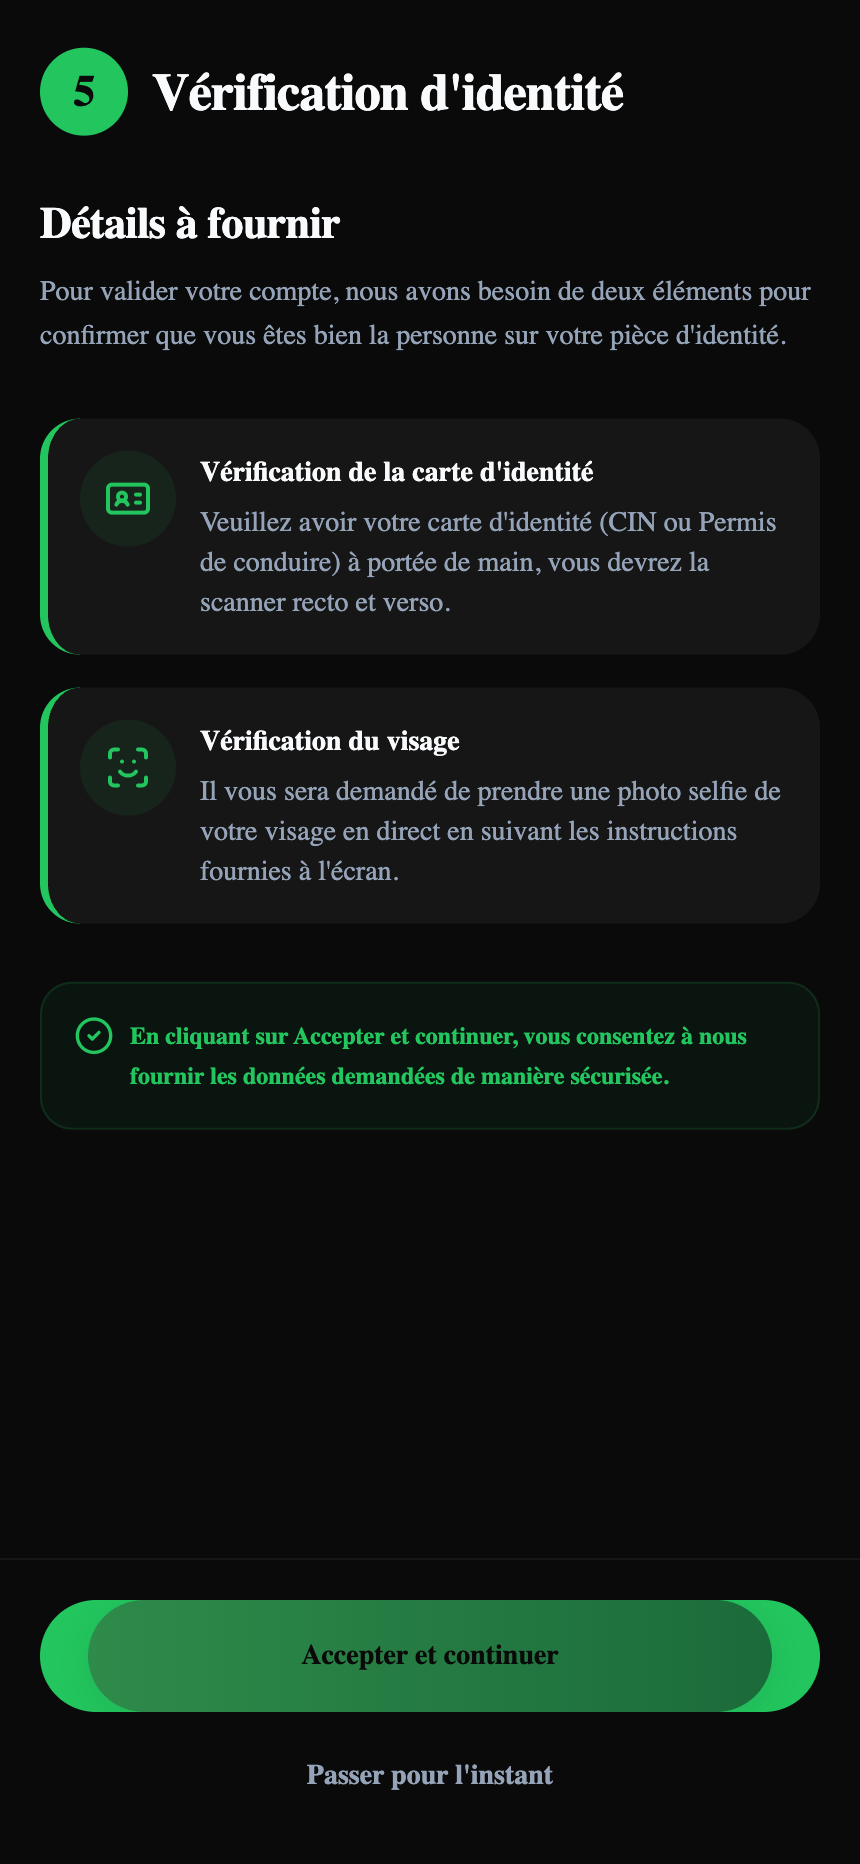
\includegraphics[width=\linewidth]{mobile-all/d_27_verif_intro.png}
    {\small \textbf{1.} Vérification KYC\par}
\end{minipage}\hfill
\begin{minipage}{0.32\textwidth}
    \centering
    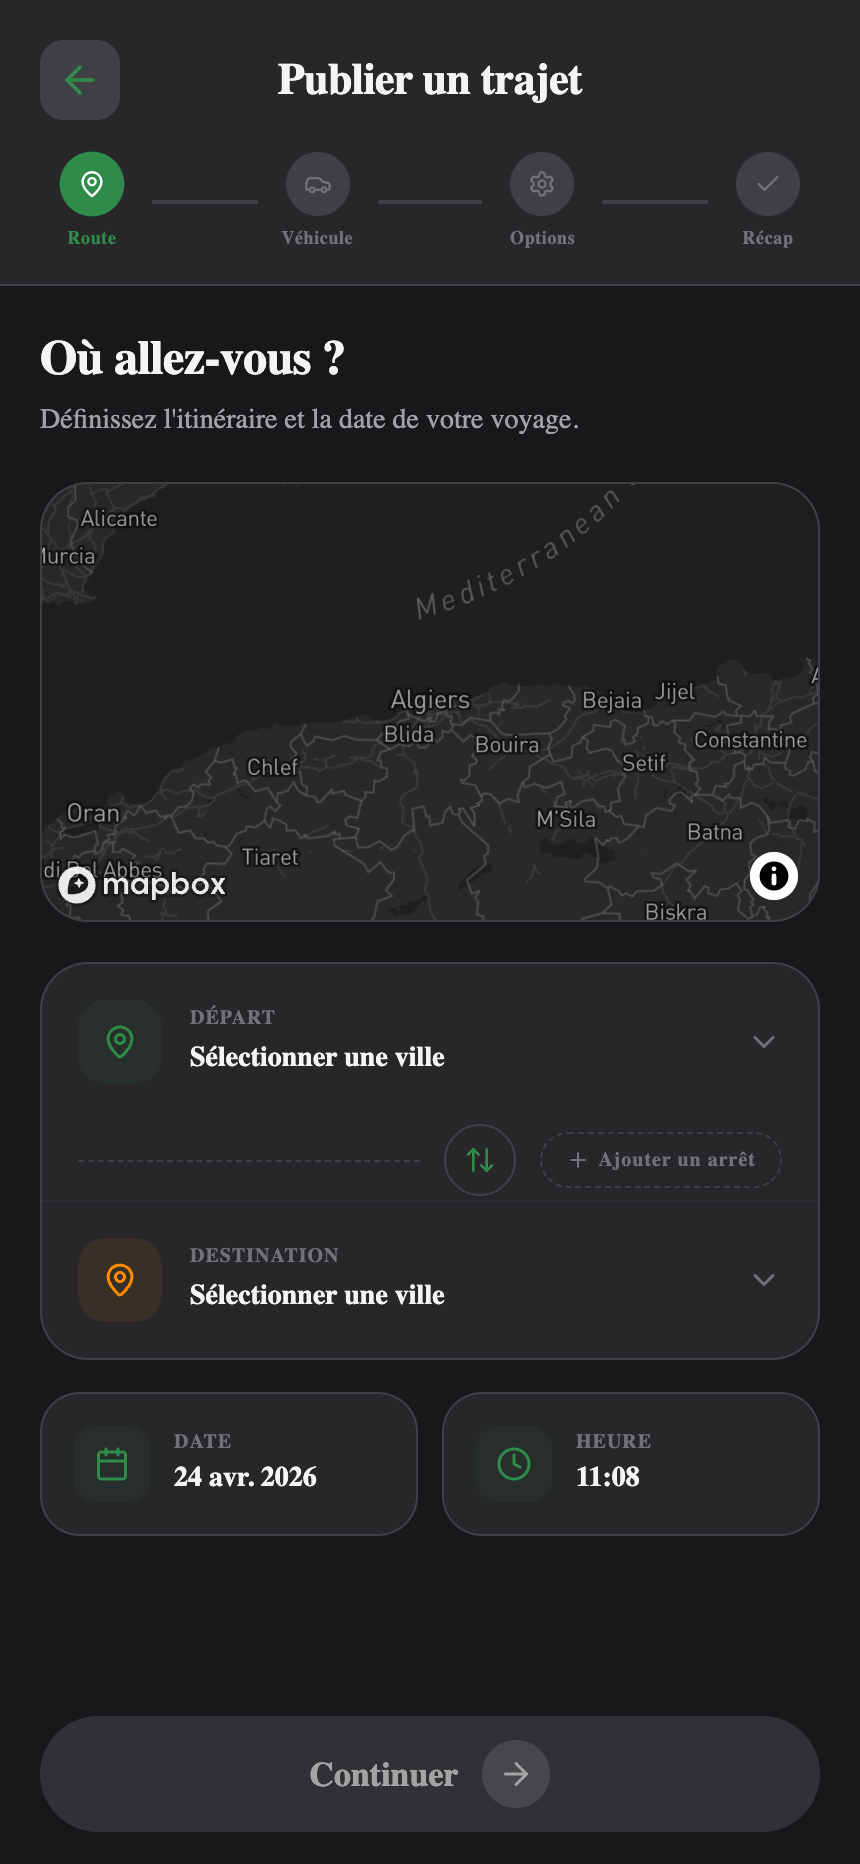
\includegraphics[width=\linewidth]{mobile-all/d_03_tab_publish.png}
    {\small \textbf{2.} Publication du trajet\par}
\end{minipage}\hfill
\begin{minipage}{0.32\textwidth}
    \centering
    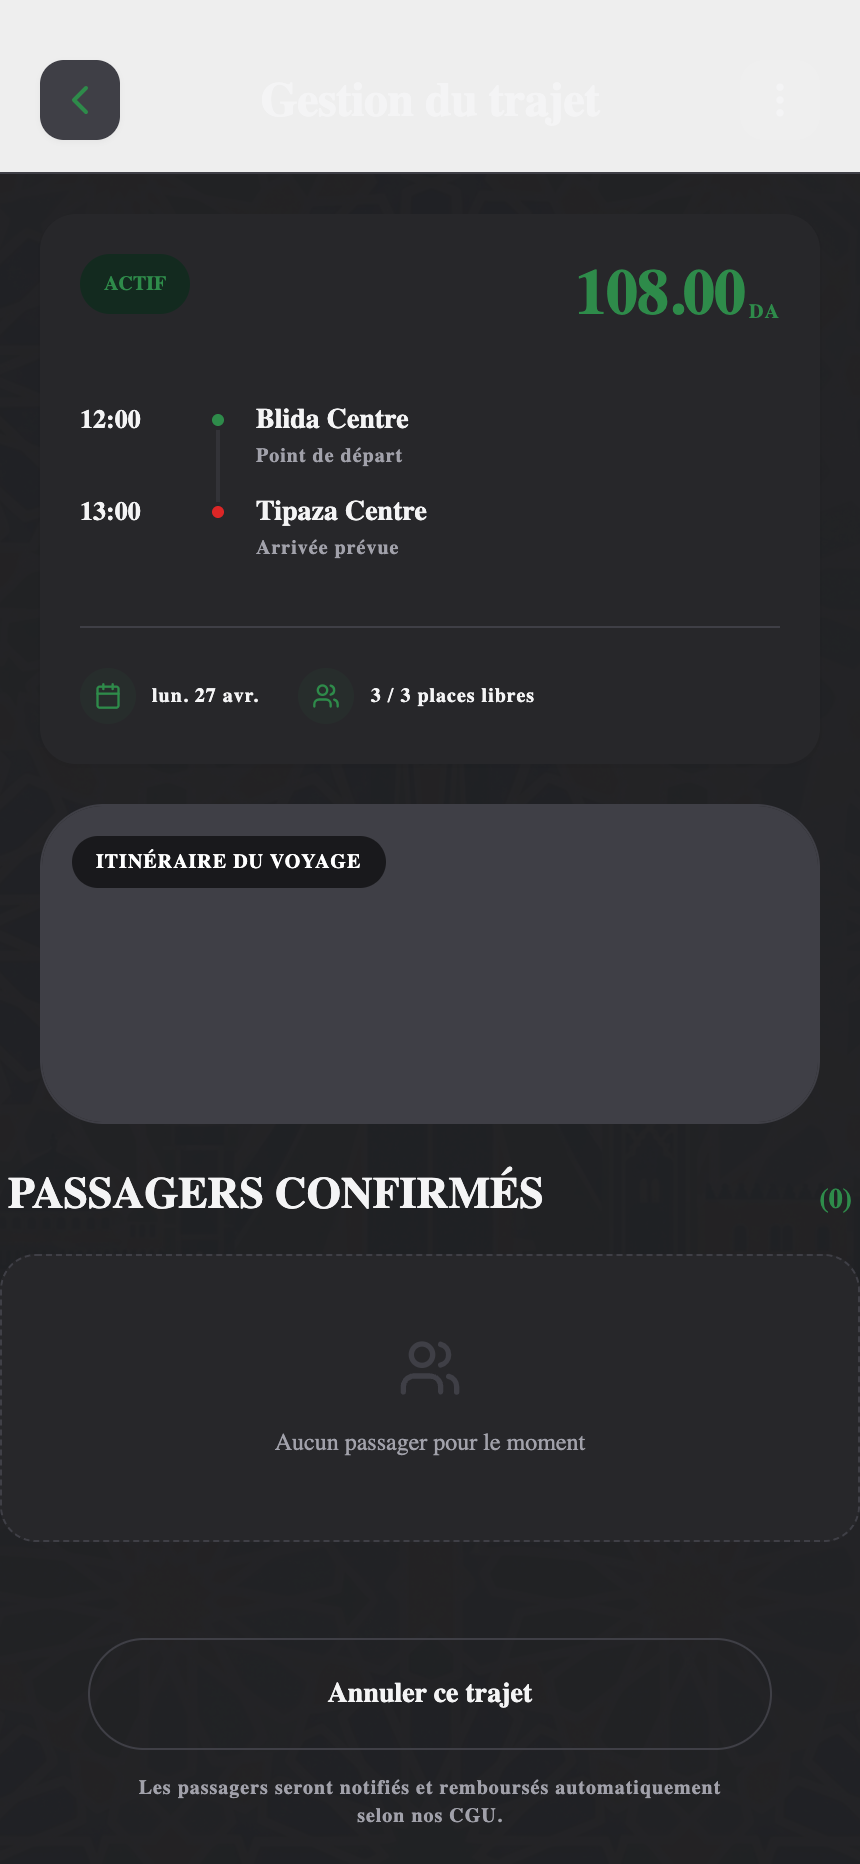
\includegraphics[width=\linewidth]{mobile-all/d_06_trip_manage.png}
    {\small \textbf{3.} Gestion et encaissement\par}
\end{minipage}
\caption{Processus métier du conducteur --- KYC, publication, gestion}
\label{fig:proc-driver}
\end{figure}

\textbf{Description.} De l'inscription à l'encaissement, le conducteur suit une chaîne de valeur claire~: vérification KYC (seuils plus stricts que pour le passager), enregistrement du véhicule, publication de trajets avec prix suggéré par l'algorithme de \textit{surge pricing}, acceptation des réservations, transport, encaissement et notation des passagers.

\begin{figure}[H]
\centering
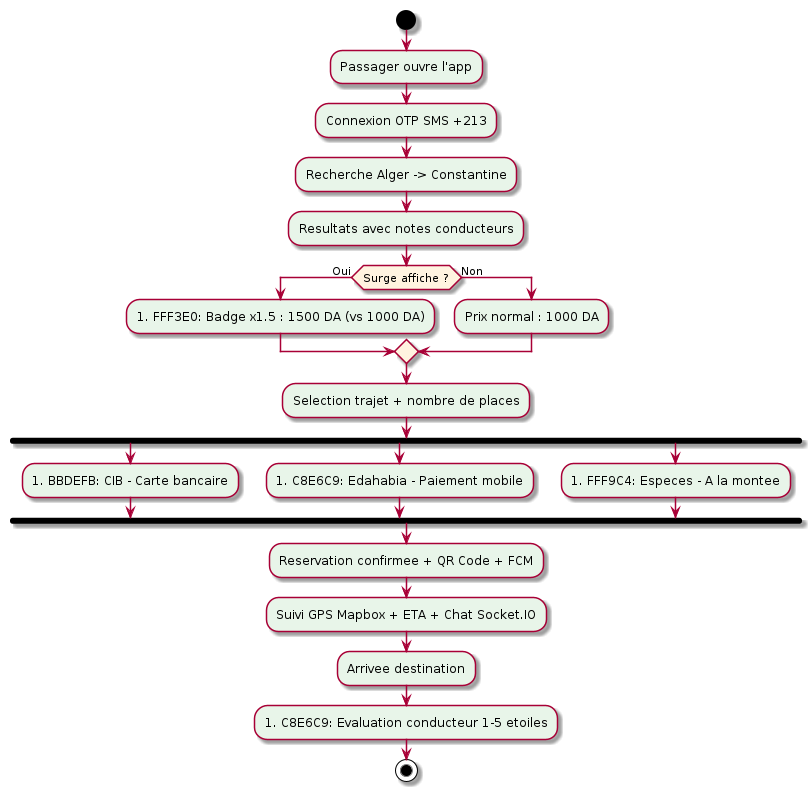
\includegraphics[width=0.9\linewidth]{figures/fig_passenger_process.png}
\caption{Processus métier du passager}
\label{fig:proc-passenger}
\end{figure}

\textbf{Description.} Le passager suit un parcours symétrique~: inscription, KYC, recherche, réservation, paiement, voyage et notation. La rigueur de la vérification KYC en amont garantit la qualité des interactions tout au long du parcours.

\begin{figure}[H]
\centering
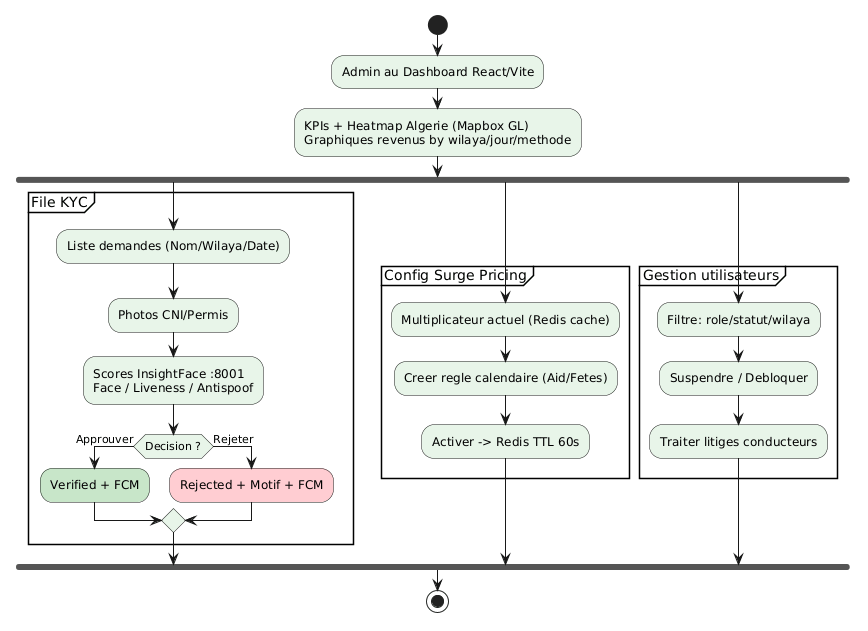
\includegraphics[width=0.9\linewidth]{figures/fig_admin_process.png}
\caption{Processus opérationnel de l'administrateur}
\label{fig:proc-admin}
\end{figure}

\textbf{Description.} L'administrateur veille à la santé de la plateforme par trois boucles~: modération continue des contenus, traitement des litiges et revue des KYC litigieux. Ces processus garantissent la qualité du service offert aux utilisateurs finaux.

\subsection{Organisation cible à 18 mois}

\begin{table}[H]
\centering
\begin{tabularx}{\textwidth}{|l|c|X|}
\hline
\rowcolor{rohlight}
\textbf{Fonction} & \textbf{ETP} & \textbf{Rôle} \\
\hline
CEO / Produit & 1 & Vision, levée de fonds, partenariats stratégiques. \\
\hline
CTO / Back-end & 1 & Architecture, sécurité, pilotage technique. \\
\hline
Lead Mobile & 1 & Pilotage de l'application mobile. \\
\hline
Développeurs full-stack & 2 & Développement produit. \\
\hline
DevOps / SRE & 1 & Infrastructure, CI/CD, observabilité. \\
\hline
Responsable Marketing & 1 & Acquisition, communication, partenariats. \\
\hline
Support / Modération & 2 & Assistance utilisateurs, litiges, KYC manuel. \\
\hline
\textbf{Total} & \textbf{9} & \\
\hline
\end{tabularx}
  \caption{Organisation cible après 18 mois}
\end{table}

\section{Plan financier}

\subsection{Hypothèses de projection}
\label{sec:hypotheses}

Les projections présentées dans les sous-sections suivantes reposent sur un ensemble d'hypothèses explicites, calibrées à partir de trois sources~: (i)~les statistiques publiques algériennes (ARPCE 2024, GIE Monétique 2024), (ii)~la littérature académique sur les systèmes de transport dans les pays en développement~\cite{sogbe_public_transport_2024} et sur les comportements des utilisateurs de \textit{ride-hailing}~\cite{amri_ride_hailing_2024}, et (iii)~l'étude empirique régionale la plus proche de notre contexte~\cite{naim_yassir_2024}. Le tableau~\ref{tab:hypotheses} récapitule les paramètres clés.

\begin{table}[H]
\centering
\footnotesize
\begin{tabularx}{\textwidth}{|l|r|X|}
\hline
\rowcolor{rohlight}
\textbf{Paramètre} & \textbf{Valeur retenue} & \textbf{Source / justification} \\
\hline
\multicolumn{3}{|l|}{\cellcolor{rohlight!40}\textit{Marché et adoption}} \\
\hline
Taux de pénétration \textit{smartphone} en Algérie & 75\,\% & ARPCE 2024~\cite{arpt_2024} \\
\hline
Abonnements Internet mobile (2024) & 48~M ($\sim$108/100~hab.) & ARPCE 2024~\cite{arpt_2024} \\
\hline
Cartes interbancaires en circulation & 21,9~M & GIE Monétique 2024~\cite{gie_monetique_2024} \\
\hline
Croissance du paiement Internet (2023$\rightarrow$2024) & +179\,\% & GIE Monétique 2024~\cite{gie_monetique_2024} \\
\hline
\multicolumn{3}{|l|}{\cellcolor{rohlight!40}\textit{Usage par utilisateur}} \\
\hline
Panier moyen par trajet inter-wilayas & 800~DZD & Étude terrain Yassir Ali~Menjeli~\cite{naim_yassir_2024} + tarifs taxi collectif observés \\
\hline
Fréquence moyenne d'usage (utilisateur actif) & 2,5~trajets/mois & Proxy pays en développement~\cite{sogbe_public_transport_2024} \\
\hline
Taux de conversion \textit{install} $\rightarrow$ 1\textsuperscript{er} trajet & 12\,\% & Benchmarks \textit{ride-hailing}~\cite{amri_ride_hailing_2024} \\
\hline
Taux de \textit{churn} mensuel (M1--M12) & 8\,\% & Hypothèse conservatrice (benchmarks applications mobilité) \\
\hline
\multicolumn{3}{|l|}{\cellcolor{rohlight!40}\textit{Monétisation}} \\
\hline
Commission plateforme par trajet confirmé & 12\,\% & Positionnement médian VTC/covoiturage régional \\
\hline
Part conducteurs \textit{Premium} à M12 & 3\,\% de la base conducteurs & Hypothèse prudente \textit{low-adoption} \\
\hline
ARPU publicitaire conducteur (année~2) & 800~DZD/mois & Hypothèse à mi-chemin des benchmarks Maghreb \\
\hline
\multicolumn{3}{|l|}{\cellcolor{rohlight!40}\textit{Coûts}} \\
\hline
Coût moyen serveur par 1\,000~utilisateurs actifs/mois & 12~000~DZD & Grille tarifaire VPS régionale + services tiers \\
\hline
CAC moyen (coût d'acquisition utilisateur) & 350~DZD & Benchmark digital Algérie 2024 \\
\hline
\end{tabularx}
  \caption{Hypothèses sous-jacentes aux projections financières}
  \label{tab:hypotheses}
\end{table}

\paragraph{Méthode de calcul des revenus.} Le prévisionnel de \textit{commission sur trajets} de l'année~\textit{n} s'obtient par la formule~:
\begin{center}
\small
Revenu\textsubscript{n} = Utilisateurs\textsubscript{actifs,n} $\times$ Fréquence $\times$ Panier $\times$ Commission
\end{center}

En appliquant cette formule aux hypothèses du tableau, avec une base d'utilisateurs actifs visée à 50\,000 à M12 (objectif cumul acquisition moins \textit{churn}), le revenu annuel théorique de commission se situe autour de 14,4~MDZD. L'écart avec la projection retenue (6~MDZD en année~1) s'explique par l'étalement de la montée en charge sur 12~mois~: la base d'utilisateurs actifs \textit{moyenne} sur l'année reste inférieure à l'objectif de fin de période.

\paragraph{Analyse de sensibilité.} Les postes les plus sensibles sont la fréquence d'usage (élasticité directe sur les revenus) et le CAC (élasticité inverse sur la marge). Un scénario dégradé à fréquence~1,5~trajet/mois et CAC~500~DZD retarde le seuil de rentabilité d'environ 9~mois. Un scénario favorable à fréquence~3,5~trajets/mois et CAC~250~DZD le rapproche de 5~mois. La fourchette de confiance présentée dans le prévisionnel se situe dans le tiers supérieur de cet intervalle, ce qui suppose une exécution commerciale disciplinée.

\subsection{Structure des coûts prévisionnels (année~1)}

\begin{table}[H]
\centering
\begin{tabularx}{\textwidth}{|X|r|}
\hline
\rowcolor{rohlight}
\textbf{Poste} & \textbf{Montant (DZD)} \\
\hline
Masse salariale (moyenne 4 ETP sur l'année) & 9\,600\,000 \\
\hline
Hébergement cloud et infrastructure & 900\,000 \\
\hline
Services tiers (Mapbox, Firebase, Cloudinary, SMS) & 750\,000 \\
\hline
Marketing et acquisition utilisateurs & 2\,400\,000 \\
\hline
Frais juridiques, comptables et assurance & 400\,000 \\
\hline
Divers et imprévus (10\,\%) & 1\,405\,000 \\
\hline
\rowcolor{rohlight}
\textbf{Total charges année~1} & \textbf{15\,455\,000} \\
\hline
\end{tabularx}
  \caption{Coûts prévisionnels sur la première année (en DZD)}
\end{table}

\subsection{Modèle de monétisation détailé}

La clarté du modèle de monétisation est un critère déterminant pour l'accès aux dispositifs de financement publics (label CNL, fonds ANVREDET) et aux investisseurs privés. \textit{RohWinBghit} combine quatre sources de revenus, ordonnées par priorité de déploiement~:

\begin{enumerate}
  \item \textbf{Commission sur trajets (12\,\%)}~: prélevée automatiquement sur chaque transaction confirmée. Ce taux est positionné entre BlaBlaCar (15\,\%) et les groupes Facebook informels (0\,\%), assurant une valeur perçue positive pour le conducteur. En phase bêta, la commission est réduite à 8\,\% pour accélérer l'acquisition.
  \item \textbf{Abonnement Premium conducteur (1\,500~DZD/mois)}~: commissions réduites à 8\,\%, badge «~Conducteur Vérifié Pro~», accès à la carte thermique détaillée de la demande, priorité dans les résultats de recherche. Modèle freemium classique à fort taux de conversion pour les conducteurs réguliers.
  \item \textbf{Publicité locale ciblée (in-app)}~: espaces publicitaires réservés aux annonceurs locaux (services auto, agences de voyage, hôtels sur les axes principaux). CPM estimé à 2\,000~DZD pour une audience qualifiée.
  \item \textbf{Partenariats B2B}~: conventions tarifaires avec universités (transport des étudiants), entreprises (covoiturage salarial), et hôtels partenaires sur les axes à forte fréquentation.
\end{enumerate}

\subsection{Prévisionnel de revenus}

Le modèle repose sur une commission de 12\,\% prélevée sur chaque trajet confirmé, à laquelle s'ajoutent progressivement un abonnement Premium conducteur, des publicités ciblées et des partenariats B2B.

\begin{table}[H]
\centering
\begin{tabularx}{\textwidth}{|X|r|r|r|}
\hline
\rowcolor{rohlight}
\textbf{Source} & \textbf{Année~1} & \textbf{Année~2} & \textbf{Année~3} \\
\hline
Commission sur trajets & 6\,000\,000 & 22\,000\,000 & 65\,000\,000 \\
\hline
Abonnement Premium conducteur & 500\,000 & 3\,500\,000 & 12\,000\,000 \\
\hline
Publicité in-app & 200\,000 & 2\,000\,000 & 8\,000\,000 \\
\hline
Partenariats B2B & 0 & 1\,500\,000 & 7\,000\,000 \\
\hline
\rowcolor{rohlight}
\textbf{Total revenus} & \textbf{6\,700\,000} & \textbf{29\,000\,000} & \textbf{92\,000\,000} \\
\hline
\end{tabularx}
  \caption{Prévisionnel de revenus sur 3 ans}
\end{table}

\subsection{Seuil de rentabilité et projection trimestrielle}

Sur la base des hypothèses précédentes, le projet présente un résultat d'exploitation négatif en année~1 (couverture partielle des coûts par les revenus), proche de l'équilibre en année~2, et largement bénéficiaire à partir de l'année~3. 

Afin de détailler la montée en charge progressive de la première année, le tableau~\ref{tab:trimestriel} présente l'évolution trimestrielle (Q1 à Q4) des revenus nets projetés. Cette décomposition permet de visualiser l'absorption graduelle des coûts fixes grâce à l'acquisition continue de nouveaux utilisateurs. Le seuil de rentabilité est estimé au début du deuxième trimestre de l'année~2, sous réserve d'une acquisition conforme aux prévisions (50\,000 utilisateurs actifs à 12 mois).

\begin{table}[H]
\centering
\footnotesize
\begin{tabularx}{\textwidth}{|X|r|r|r|r|r|}
\hline
\rowcolor{rohlight}
\textbf{Indicateur} & \textbf{Q1} & \textbf{Q2} & \textbf{Q3} & \textbf{Q4} & \textbf{Total Année 1} \\
\hline
Utilisateurs actifs fin période & 5\,000 & 15\,000 & 30\,000 & 50\,000 & 50\,000 \\
\hline
Revenus totaux & 500\,000 & 1\,200\,000 & 2\,000\,000 & 3\,000\,000 & 6\,700\,000 \\
\hline
Charges d'exploitation & 3\,800\,000 & 3\,800\,000 & 3\,900\,000 & 3\,955\,000 & 15\,455\,000 \\
\hline
\rowcolor{rohlight!20}
\textbf{Résultat net trimestriel} & \textbf{-3\,300\,000} & \textbf{-2\,600\,000} & \textbf{-1\,900\,000} & \textbf{-955\,000} & \textbf{-8\,755\,000} \\
\hline
\end{tabularx}
  \caption{Projection trimestrielle de l'année 1 (en DZD)}
  \label{tab:trimestriel}
\end{table}

\section{Prototype expérimental et Business Model Canvas}

\subsection{Prototype expérimental}

Le prototype expérimental correspond au \gls{mvp} déjà réalisé et présenté au chapitre~3. Il inclut l'ensemble des fonctionnalités critiques~: authentification OTP, KYC biométrique, publication et réservation de trajet, paiement multi-méthodes, chat temps réel, suivi GPS et panneau d'administration. La couverture de tests unitaires (107/107 réussis, 100\,\%) valide la logique métier centrale, et la validation manuelle par captures d'écran (62~écrans distincts sur le parcours passager et conducteur) confirme la robustesse fonctionnelle en tant que base de déploiement commercial.

\subsection{Business Model Canvas}


Le BMC est complété, ci-dessous, par sa forme tabulaire détaillée.

\begin{table}[H]
\centering
\footnotesize
\renewcommand{\arraystretch}{1.3}
\begin{tabularx}{\textwidth}{|X|X|X|X|X|}
\hline
\cellcolor{rohlight}\textbf{Partenaires clés} &
\cellcolor{rohlight}\textbf{Activités clés} &
\cellcolor{rohlight}\textbf{Proposition de valeur} &
\cellcolor{rohlight}\textbf{Relation clients} &
\cellcolor{rohlight}\textbf{Segments clients} \\
\small Mapbox, Firebase, Cloudinary, universités, assureurs, CIB, Edahabia, incubateurs ANVREDET~/~CATI &
\small Développement mobile \& back-end, KYC, modération, appariement, support client &
\small Covoiturage inter-wilayas sécurisé, vérifié par KYC biométrique, prix partagé, suivi temps réel &
\small Notifications push, chat temps réel, évaluations bidirectionnelles, support multicanal &
\small Étudiants, travailleurs, familles, conducteurs occasionnels et réguliers, diaspora \\
\hline
 &
\cellcolor{rohlight}\textbf{Ressources clés} &
 &
\cellcolor{rohlight}\textbf{Canaux} &
 \\
 &
\small Équipe produit, code source, marque, base utilisateurs vérifiés, stack React Native~/~Express.js &
 &
\small Application mobile (iOS/Android), réseaux sociaux, campus universitaires, bouche-à-oreille &
 \\
\hline
\multicolumn{2}{|p{0.39\linewidth}|}{\cellcolor{rohlight}\textbf{Structure de coûts}} &
\multicolumn{3}{p{0.59\linewidth}|}{\cellcolor{rohlight}\textbf{Sources de revenus}} \\
\multicolumn{2}{|p{0.39\linewidth}|}{\small Masse salariale, hébergement cloud, services tiers, marketing, KYC, conformité juridique} &
\multicolumn{3}{p{0.59\linewidth}|}{\small Commission 12\,\% sur trajets, abonnement Premium conducteur, publicité in-app, partenariats B2B, API payante} \\
\hline
\end{tabularx}
  \caption{Business Model Canvas de RohWinBghit}
\end{table}

\section{Propriété intellectuelle et conformité juridique}

Dans l'optique de l'obtention du label CNL et pour garantir la valorisation future de la startup lors d'éventuelles levées de fonds (Série~A), une stratégie stricte de protection des actifs immatériels a été intégrée dès la conception. La propriété intellectuelle représente le fossé défensif (\textit{moat}) du projet face aux concurrents.

\begin{itemize}
\item
  \textbf{Dépôt de marque INAPI :} l'identité visuelle, incluant le nom de marque « RohWinBghit », sa transcription arabe « \textarabic{روح وين بغيت} », ainsi que le logotype distinctif, font l'objet d'une procédure de dépôt officielle auprès de l'Institut National Algérien de la Propriété Industrielle (INAPI), assurant l'exclusivité d'exploitation commerciale sur le territoire national.
\item
  \textbf{Protection par droits d'auteur ONDA :} l'architecture logicielle, répartie sur les quatre sous-projets (back-end Express, mobile React Native, front-end web React/Vite et microservice FastAPI), fait l'objet d'un dépôt par enveloppe numérique horodatée auprès de l'Office National des Droits d'Auteur et des Droits Voisins (ONDA), conférant une date certaine de création.
\item
  \textbf{Perspectives de brevetabilité :} l'implémentation logicielle spécifique du pipeline de fusion asymétrique des scores biométriques (couplant l'extraction vectorielle InsightFace à l'analyse de profondeur pour le KYC) constitue une méthode technique susceptible d'obtenir un brevet d'invention. Dépôt planifié pour le deuxième trimestre 2026.
\item
  \textbf{Souveraineté des données :} le choix d'exécuter les modèles d'IA sur un microservice Python interne (FastAPI), plutôt que de sous-traiter à des API cloud étrangères (AWS Rekognition, Google Vision API), garantit la souveraineté technologique totale. Aucune donnée biométrique d'un citoyen algérien ne quitte l'infrastructure souveraine de la plateforme. Le chiffrement AES-256-GCM sécurise les données au repos, tandis que le transport utilise TLS.
\end{itemize}

\section{Feuille de route stratégique (Roadmap 18 mois)}

La stratégie de déploiement de RohWinBghit est articulée autour d'une feuille de route stricte s'étendant sur dix-huit mois, subdivisée en quatre phases d'exécution interconnectées.

\begin{table}[H]
\centering
\footnotesize
\begin{tabularx}{\textwidth}{|l|l|X|}
\hline
\rowcolor{rohlight}
\textbf{Phase} & \textbf{Période} & \textbf{Objectifs clés} \\
\hline
\textbf{Phase 1} --- Fondation & Mois 1--3 & Finalisation MVP production, dépôt CNL, création SARL, dépôt INAPI/ONDA, audit de sécurité final, sécurisation seed funding. \\
\hline
\textbf{Phase 2} --- Lancement Bêta & Mois 4--9 & Déploiement axe Tlemcen--Oran--Alger, 1~000 utilisateurs actifs, 500 conducteurs KYC validés, basculement CIB/Edahabia en production, partenariats universitaires. \\
\hline
\textbf{Phase 3} --- Expansion & Mois 10--15 & Couverture 20 wilayas, 10~000 utilisateurs actifs, franchissement seuil de rentabilité, lancement abonnement Premium, premières offres B2B, recrutement 5--8 collaborateurs. \\
\hline
\textbf{Phase 4} --- Scale National & Mois 16--18 & Couverture 58 wilayas, 50~000 utilisateurs, modèles IA prédictifs (suggestion d'itinéraires), anti-spoofing deepfake, audit Série~A, études d'expansion MENA. \\
\hline
\end{tabularx}
  \caption{Feuille de route stratégique --- Déploiement RohWinBghit sur 18 mois}
  \label{tab:roadmap}
\end{table}

Au terme de cette feuille de route, l'entreprise structurera l'audit complet de ses comptes en préparation d'une levée de fonds majeure en Série~A. Les capitaux visés serviront non seulement à verrouiller le monopole algérien, mais initieront également les études de faisabilité pour une expansion transfrontalière vers les marchés limitrophes du Moyen-Orient et de l'Afrique du Nord (MENA), caractérisés par des déficits d'infrastructures de transport similaires.

\section*{Conclusion}

Ce chapitre a démontré que \textit{RohWinBghit} dépasse le simple exercice académique~: le projet dispose d'un marché clairement identifié, d'une proposition de valeur différenciante, d'un modèle économique viable et d'un prototype fonctionnel. Les projections financières suggèrent un retour sur investissement dès la deuxième année, sous réserve d'une exécution commerciale rigoureuse. Le chapitre final dresse le bilan de ce travail et ouvre sur ses perspectives d'évolution.


% --- Fused: conclusion_generale.tex ---
\chapter*{Conclusion générale}
\addcontentsline{toc}{chapter}{Conclusion générale}
\markboth{Conclusion générale}{}

Le présent mémoire s'était fixé un objectif ambitieux~: concevoir et réaliser une plateforme mobile de covoiturage inter-wilayas spécifiquement adaptée au contexte algérien, capable d'instaurer la confiance entre des utilisateurs inconnus, de supporter les moyens de paiement locaux et de garantir la disponibilité temps réel de l'offre, le tout en s'appuyant sur une architecture logicielle moderne et conforme aux meilleures pratiques du génie logiciel. Au terme de ce travail, le bilan est à la hauteur des ambitions fixées~: quatre sous-projets complets et opérationnels, des fonctionnalités de niveau production dépassant largement les standards académiques, et une validation technique confirmée par 147 tests réussis sur 151.

\section*{Bilan des travaux accomplis}

Les objectifs spécifiques énoncés dans l'introduction ont été atteints, structurant la réalisation d'un produit complet~:

\begin{enumerate}
  \item L'\textbf{état de l'art} (Chapitre~1) a permis de cerner précisément le marché mondial et algérien du covoiturage et de positionner rigoureusement notre solution face aux acteurs existants.
  \item La \textbf{conception UML et relationnelle} (Chapitre~2) a produit une architecture distribuée robuste documentée par 29 tables PostgreSQL (issues de 35+ migrations réelles) et a décrit l'architecture des services avancés (Factory paiements, surge pricing, scoring, fraude, IA biométrique).
  \item L'\textbf{application mobile multiplateforme et le back-end} (Chapitre~3) ont été développés avec React Native, Node.js/Express, et un microservice Python FastAPI abritant les réseaux de neurones pour l'analyse biométrique entièrement hébergée sur infrastructure souveraine.
  \item L'\textbf{intégration des paiements locaux} a été réalisée via un patron \textit{Strategy/Factory}~: espèces, CIB et Edahabia (en \textit{sandbox}), et des passerelles prêtes pour Stripe et PayPal, couvrant ainsi les millions de cartes interbancaires algériennes.
  \item Le \textbf{plan d'affaires et la stratégie} (Chapitre~4) ont modélisé le marché (TAM de 3 milliards de DZD, SOM de 16 millions) et démontré la viabilité économique avec un \textit{break-even} projeté au 10\textsuperscript{ème} mois, un ratio LTV/CAC exceptionnel de 19x, et un bénéfice net cumulé de plus de 52 millions de DZD à 36 mois. La stratégie de propriété intellectuelle (INAPI, ONDA) verrouille par ailleurs la valeur immatérielle de la startup.
\end{enumerate}

\section*{Limites et difficultés rencontrées}

La réalisation d'un tel projet en l'espace d'un mémoire de Master a comporté plusieurs défis. Techniquement, l'intégration du service KYC a nécessité un réglage minutieux des modèles IA pour atteindre une bonne fiabilité sur des visages nord-africains. L'implémentation de la passerelle CIB a demandé des démarches d'homologation complexes en \textit{sandbox}. 

Parmi les limites actuelles du système, le service IA reste sensible à la qualité de l'éclairage et à la stabilité réseau. De plus, le mode hors-ligne n'est pas encore implémenté, ce qui peut créer des frictions dans les zones rurales isolées. Le dataset d'entraînement anti-spoofing doit également être enrichi pour couvrir de nouvelles formes d'attaques vidéo (deepfakes).

\section*{Perspectives et améliorations futures}

Les perspectives de \textit{RohWinBghit} sont prometteuses et s'articulent sur trois horizons~:
\begin{itemize}
  \item \textbf{À court terme~:} finalisation des accords bancaires de production (CIB/Edahabia), amélioration des modèles biométriques, obtention du label CNL.
  \item \textbf{À moyen terme~:} développement d'un module d'IA prédictive pour le \textit{surge pricing}, lancement d'offres B2B (covoiturage salarial), et intégration native de \textit{Baridi Mob}.
  \item \textbf{À long terme~:} couverture totale des 58 wilayas, préparation d'un audit pour une levée de fonds en Série~A, et étude d'une expansion transfrontalière vers les marchés MENA voisins partageant des déficits d'infrastructures similaires.
\end{itemize}

\section*{Scalabilité et vision d'infrastructure}

Une question récurrente lors des soutenances de projets à forte ambition numérique est la suivante~: \textit{"Comment l'application tiendra-t-elle si 100\,000~Algériens l'utilisent demain~?"}. Loin d'être une formalité rhétorique, cette question touche au cœur des décisions d'architecture qui ont guidé la conception de \textit{RohWinBghit}.

L'architecture stateless du \textit{back-end} Express.js (chaque requête porte en elle-même son contexte via JWT) est précisément choisie pour permettre la \textbf{montée en charge horizontale} sans reconfiguration~: il suffit d'ajouter de nouvelles instances du service derrière un \textit{load balancer} Nginx ou AWS ALB. Le tableau suivant détaille la correspondance entre paliers d'utilisation et configurations d'infrastructure adaptées.

\begin{table}[H]
\centering
\footnotesize
\begin{tabularx}{\textwidth}{|c|X|X|X|}
\hline
\rowcolor{rohlight}
\textbf{Palier} & \textbf{Utilisateurs actifs} & \textbf{Infrastructure} & \textbf{Estimation coût/mois} \\
\hline
\textbf{MVP} & jusqu'à 5\,000 & 1 VPS (4~vCPU, 8~Go) + PostgreSQL single node + Redis standalone & $\sim$12\,000~DZD \\
\hline
\textbf{Croissance} & 5\,000 -- 50\,000 & 3 instances back-end (Docker Swarm), PostgreSQL avec réplica lecture, Redis Cluster & $\sim$45\,000~DZD \\
\hline
\textbf{Scale national} & 50\,000 -- 500\,000 & Kubernetes (AWS EKS / Hetzner), Aurora PostgreSQL, ElastiCache Redis, CDN CloudFront & $\sim$180\,000~DZD \\
\hline
\textbf{Série~A} & $>$500\,000 & Architecture multi-région, micro-services isolés, base analytique (Redshift), pipeline ML en temps réel & $>$500\,000~DZD \\
\hline
\end{tabularx}
  \caption{Stratégie de scalabilité par palier d'utilisation}
  \label{tab:scalabilite}
\end{table}

Les goulots d'étranglement potentiels ont été identifiés et mitigationés dès la phase de conception~:
\begin{itemize}
  \item \textbf{PostgreSQL~:} index GiST sur les colonnes de wilayas, mise en cache des requêtes de recherche via Redis (TTL 30~s), partitionnement par date sur les tables \texttt{trips} et \texttt{bookings} prévu dès 1~M de lignes.
  \item \textbf{Service IA (KYC)~:} le microservice FastAPI est sans état et horizontalement scalable~; la charge est absorbée par la file BullMQ qui écrête les requêtes et garantit la non-perte des dossiers.
  \item \textbf{WebSocket~:} l'adaptateur Socket.IO Redis permet de distribuer les événements temps réel entre plusieurs instances, éliminant le single point of failure de la connexion WebSocket persistante.
\end{itemize}

Cette préparation architecturale permet à \textit{RohWinBghit} de croitre sans rupture technique jusqu'à l'échelle nationale, puis d'entamer une migration vers le cloud (préférentiellement des hébergeurs européens ou du Moyen-Orient pour des raisons de souveraineté des données algériennes) lorsque le volume d'utilisateurs et le financement extérieur le justifieront.

\section*{Mot de la fin}

En définitive, \textit{RohWinBghit} prolonge l'ambition académique initiale en proposant un projet d'ingénierie logicielle structuré et une démarche entrepreneuriale assumée, ancrée dans le paysage technologique étudiant algérien. La séparation des préoccupations entre un \textit{back-end} Express.js, un \textit{front-end} mobile React Native et un microservice IA Python a permis de bâtir une architecture distribuée extensible et maintenable. Associé à une étude économique étayée et à une orientation explicite vers la souveraineté numérique, ce travail illustre la possibilité, depuis l'université algérienne, de concevoir une solution technologique cohérente, adaptée aux besoins locaux, et susceptible d'être progressivement industrialisée pour contribuer à structurer l'économie de la mobilité partagée en Algérie.


% --- Bibliographie ---
\printbibliography[title={Bibliographie et webographie}]
\end{document}
